\documentclass{tudelft-report}
\usepackage{amsmath}
\usepackage{multirow}
\usepackage{pifont}
\usepackage{hyperref}
\usepackage{url}
\usepackage{svg}
\usepackage{pdfpages,caption}
\usepackage[toc,page]{appendix}
\usepackage{array}
\usepackage{blindtext}
\usepackage{wrapfig}
\usepackage[export]{adjustbox}
\usepackage{stackengine}
\usepackage{graphicx}
\usepackage[export]{adjustbox}
\usepackage[parfill]{parskip}
\usepackage{siunitx}
\usepackage[noabbrev]{cleveref}
\usepackage{subcaption}
\usepackage{mathtools}
\usepackage{multirow}
\usepackage{relsize}
\usepackage{tabularx}

\captionsetup{compatibility=false}
\newcommand{\norm}[1]{\left\lVert#1\right\rVert}
\begin{document}

%% Use Roman numerals for the page numbers of the title pages and table of
%% contents.
\frontmatter

%% Uncomment following 19 lines for a cover with a picture on the lower half only
%\title[tudelft-white]{Title}
%\subtitle[tudelft-cyan]{Optional subtitle}
%\author[tudelft-white]{J.\ Random Author}
%\affiliation{Technische Universiteit Delft}
%\coverimage{cover.jpg}
%\titleoffsetx{10cm}
%\titleoffsety{10cm}
%\afiloffsetx{1cm}
%\afiloffsety{18cm}
%\covertext[tudelft-white]{
%    \textbf{Cover Text} \\
%    possibly \\
%    spanning 
%    multiple 
%    lines
%    \vfill
%    ISBN 000-00-0000-000-0
%}
%\makecover

%% Uncomment following 16 lines for a cover with a picture on the lower half only
\title[Master Thesis]{Placeholder Title}
\author{C.\ Christoforidis}
\affiliation{Technische Universiteit Delft}
\coverimage{images/cover_thesis.jpg}
\covertext{
    \textbf{Cover Text} \\
    possibly \\
    spanning 
    multiple 
    lines
    \vfill
    ISBN 000-00-0000-000-0
}

\makecover


%% Include an optional title page.
\begin{titlepage}

    \begin{center}
    
    %% Insert the TU Delft logo at the bottom of the page.
    \begin{tikzpicture}[remember picture,overlay]
        \node at (current page.south)[anchor=south,inner sep=0pt]{
            
\includegraphics{cover/logo}
        };
    \end{tikzpicture}
    
    %% Extra whitespace at the top.
    \vspace*{2\bigskipamount}
    
    %% Print the title in cyan.
    {\makeatletter
    \titlestyle\color{tudelft-cyan}\Huge\@title
    \makeatother}
    
    %% Print the optional subtitle in black.
    {\makeatletter
    \ifx\@subtitle\undefined\else
        \bigskip
        \titlefont\titleshape\LARGE\@subtitle
    \fi
    \makeatother}
    
    \bigskip
    \bigskip
    
    by
    %door
    
    \bigskip
    \bigskip
    
    %% Print the name of the author.
    {\makeatletter
    \titlefont\Large\bfseries\@author
    \makeatother}
    
    \vfill
    
    in partial fulfillment of the requirements for the degree of
    %in overeenstemming met de vereisten voor het verkrijgen van de graad van
    
    \bigskip
    \bigskip
    
    {\bfseries Master of Science}
    
    in Biomedical Engineering
    
    \bigskip
    \bigskip
    
    at the Delft University of Technology.
    %aan de Technische Universiteit Delft,
    
    %to be defended publicly on Tuesday January 1, 2013 at 10:00 AM.
    %in het openbaar de verdedigen op dinsdag 1 januari om 10:00 uur.
    
    \vfill
    
    \begin{tabular}{lll}
    %% Add additional information here, per faculty requirements, e.g
        Student number: & 4737822 \\
        Project duration: & \multicolumn{2}{l}{ 2018 -- 2019} \\
        Supervisor: & Dr.\ ir.\ A.L.\ Schwab, & TU Delft \\
        Thesis committee:
            & Dr.\ ir.\ R.\ Happee, & TU Delft \\
            & MSc.\ G.\ Dialynas, & TU Delft \\
    \end{tabular}
    
    %% Only include the following lines if confidentiality is applicable.
    \bigskip
    \bigskip
    \emph{This thesis is confidential and cannot be made public until May, 2019.}
    %\emph{Op dit verslag is geheimhouding van toepassing tot en met 31 december 2013.}
    
    \bigskip
    \bigskip
    \copyright2019\\
    C. Christoforidis\\
    ALL RIGHTS RESERVED
    An electronic version of this thesis is available at \url{http://repository.tudelft.nl/}.
    %Een elektronische versie van dit verslag is beschikbaar op \url{http://repository.tudelft.nl/}.
    
    \end{center}
    
    \end{titlepage}
    
    

\chapter*{Abstract}\label{chap:abstract}
\setheader{Abstract}

Bicycle riding is a fundamental part of everyday transportation in many countries around the world. Ever since the development of the safety bicycle, the bicycle remains  one of the most prominent means of transport. Despite cycling’s prominence in every day life for almost two centuries we still do not fully understand how the rider controls the bike in a more systematic way.

The purpose of this literature study is to explore and evaluate models of the single track vehicle rider found in the researched bibliography. Firstly a brief analysis of bicycle stability and its dynamics is presented as explored by Meijaard et al.\cite{meijaard2007linearized}. In Chapter \ref{results}models which were classified on their control theory approach are presented. In section \ref{ch:classical}, models using the classical control approach are described. Following the steps of early cybernetics research in which airplane pilot modelling was pioneered by McRuer\cite{mcruer1959human,mcruer1967manual,mcruer1967manual2}, a plethora of authors attempted adapting McRuers crossover model in order to model the rider of a seemingly much more complex task, motorcycle and bicycle riding. However some argued that such an approach will not work since cycling is not just a compensatory task. These spawned a new wave of research focusing in optimal control which is described in section \ref{ch:optimal}.  This approach has its roots in early motor control research in which the human brain is believed to work as a constrained optimal controller. In the final section of Chapter \ref{results}, all models that do not fall under the two approaches described above are reviewed. These include fuzzy logic controllers which have the advantage of incorporating heuristic  findings that are impossible to formulate using systematic mathematical approaches. Also intermittent control is briefly explored as a solution. 

Based on this literature review the graduation project will try to model the human controller for bicycles, while focusing  on the roll stabilization task. Open road experiments will be conducted in effort to estimate the controller’s parameters and indirectly validate it with real cycling data.



\begin{flushright}
{\makeatletter\itshape
    \@author \\
    Delft, April 2018
\makeatother}
\end{flushright}


\tableofcontents

%% Use Arabic numerals for the page numbers of the chapters.
\mainmatter

\chapter{Introduction}
\label{introduction}

Bicycle riding is a fundamental part of everyday transportation in many countries around the world. Ever since the development of the safety bicycle(two equal sized wheels, pneumatic tires, chain drive, rear wheel propulsion and a bent front fork), almost 130 years ago, the bicycle remains  one of the most prominent means of transport \cite{kooijman2013review}. With the growing concerns of sedentary lifestyles many choose the bicycle as their primary commute vehicle with the hopes of maintaining some levels of fitness. Additionally the bicycle is the preferred means of physical exercise for the elderly especially in the Netherlands and Denmark. Despite the fact that riding a bicycle is one of the first skills we acquire as kids and is used throughout the adult life, the fundamental way humans control the bicycle and ,generally single track vehicles,  is yet to be understood.\par
In a recent study examining the entries of patients to the emergency department due to traffic related accidents in the Netherlands (see Fig. \ref{fig:figure1}), it was found that bicycle related accidents were the most prevalent. With over 60,000 reported cases  bicycle accidents outnumber automobile accidents more than 4 to 1. It therefore  becomes clear that a lot could be done to improve cycling safety. Further look at the figure will reveal that most of those accidents did not involve a second party. There was  just a rider that fell off his bike. Although there are several potential reasons that riders lose control of the bicycle, formulating a general model of  how humans control single track vehicles could prove invaluable in understanding the causes behind the above numbers.

\begin{figure}[ht]
    \centering
    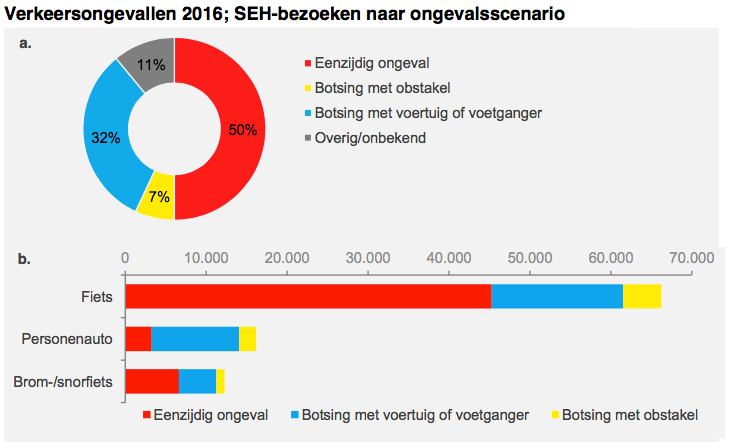
\includegraphics[scale=0.8]{images/figure1_1.png}
    \caption[Short title]{The number of road users that visit the emergency department at a hospital after a traffic accident in the Netherlands in 2016. Red indicates single vehicle accidents, yellow indicates a collision with an obstacle, blue indicates multi-vehicle accident and grey indicates other type of accidents\cite{krul_nijman_stam_2016}.}
    \label{fig:figure1}
\end{figure}

Following the steps of early cybernetics research in which airplane pilot modelling was pioneered by McRuer\cite{mcruer1959human,mcruer1967manual,mcruer1967manual2}, a plethora of authors attempted adapting McRuers crossover model in order to model the rider of a seemingly much more complex task; motorcycle and bicycle riding. However, some argued that such an approach will not work since cycling is not just a compensatory task. Moreover little concern was made to the fact that humans try to optmize for perfomance while simultaneously exerting the lowest amount of control effort. These spawned a new wave of research focusing in optimal control.  This approach is based in early motor control research in which the human brain is believed to work as a constrained optimal controller. 

A further look in motor control research will reveal the importance of the inernal model in control, state estimation and dead time compensation \cite{francis1976internal, garcia1982internal, wolpert1995internal, gillespie2016human}. The inernal model  theory argues that the motor system is controlled by the constant interactions between the process and the controller. In this case the process is the body, however in tasks like cycling the bicycle can be considered as an extension of the body. The internal model can be used either as a tool for control in the form of the inverse model \cite{edelmann2015,getz1995internal} or as a forward model in state estimation in combination with Kalman filters \cite{wolpert1995internal}. Additionally, forward models can be used in delay compensation algorithms \cite{miall1993cerebellum,van2001adaptive}. 

In this work an attempt to iterate over existing rider control models is made with the goal of answering two important questions. 
\begin{itemize}
        \item How signficiant is the effect of torque feedback for the balance task of bicycling?
        \item What is the prediction strategy best suitable for dead time  compensation in the balance task of bicycling?
\end{itemize}

In order to answer the above questions system identification techniques are employed using  the experimental dataset acquired within the scope of this thesis. In \cref{chapter2} an attempt is made to investigate the effect of haptic feedback in the task of balancing a bicycle under lateral perturbations. Non-parametric identification was conducted on the response of 20 riders in two different experimental conditions. In the first one the experimental bicycle operated as a normal bike while in the second the coupling between roll and steer was modified in order to cancel the torque feedback that would naturally transfer from the front wheel contact point to the handlebars. In \cref{hapticFB} further analysis is conducted by applying gray box identification techniques in order to investigate again the importance of torque feedback but also to test the effect of time delays in sensory feedback pathways and how these can be compensated throught the use of inernal model theory. In \cref{app:A,app:B,app:C} further details are presented on the methodology used to acquire proper measurments from the sensors of the experimental platform.


% Every human-machine system requires an understanding of how the plant operates. In the case of the bicycle multiple efforts have been made in capturing the dynamics of the bicycle and its  self-stabilizing behavior. These have resulted in a set of linearized equations of motion, now  commonly referred to as the Whipple Carvalho model \cite{meijaard2007linearized}, which is going to be discussed further in chapter \ref{results}.\par
% As it is known single track vehicles are not stable at low speeds. This is why a controller (like the human rider) is required to close the loop and create a stable system. There are two ways with which the human affects the dynamics of the plant. The first is with its passive interactions with the plant as a physical multibody system. Most passive models model the rider as a point mass rigidly attached to the rear frame, or as a pendulum connected to the rear frame \cite{eaton1975man}, although recent efforts have been made to extend this further with more complex passive rider models which include modeling of neuromuscular dynamics with spring-damper systems at various interfaces between rider and the bicycle frame\cite{dialynas2019}. The second is with its active control behavior. This involves the active control motion, such as steering, leaning or pedaling, applied by the rider to control and balance the bicycle. In most such cases, the passive behavior  of the rider is simplified by only  accounting for a fixed mass on the seat post, but when lean torque needs to be examined more complex modeling is required. The focus of the study is to explore the available models that best express the human rider as a controller in the bicycle-rider closed loop system.\par
% The literature review presented herein gives an overview of research done in the field of active rider modelling  concerning single-track vehicles, while discussing with which methods and to what extent have these models been validated. This extensive overview is given in section \ref{sub:rider} of chapter \ref{results}, which is structured in three sections: \ref{ch:classical} Classical control system design, \ref{ch:optimal} Optimal control system design and \ref{ch:other} Other control system design. Chapter \ref{conclusions} concludes on the results from Chapter \ref{results} having as a final goal to answer the research question:
% \par
% • \textbf{What is the controller that best simulates the behavior of the human in the control of single track vehicles?}


\chapter{The effect of haptic feedback in the balance task of bicycling}\label{chapter 5}

%\textcolor{black}{->Corresponding article: G. Dialynas, R. Happee, A. L. Schwab, The importance of steering feedback in the balance and maneuver of a bicycle, Vehicle System Dynamics \textcolor{red}{ONGOING} possible submission day: \textcolor{red}{1st of March 2019}}}

\footnotemark{Corresponding article: G. Dialynas,C. Christoforidis, R. Happee, A. L. Schwab, The effect of haptic feedback in the balance task of bicycling, In Proceedings of the 4th Triannual International Bicycle and Motorcycle Dynamics Conference (2019).}


\section{Abstract}

The objective of this research is to study the effect of haptic steering feedback on the balancing task of a bicycle during lateral perturbation tests, in an effort to improve two-wheeler safety. The steer-by-wire bicycle designed and built at TU Delft bicycle laboratory is used as an experimental platform to analyze the rider response with and without steering feedback. The response of the rider's control actions is represented in the time domain by means of impulse response functions (IRFs). More specifically, three metrics are defined  in order to assess both steering and balancing performance. Results failed to indicate any statistically significant difference between experimental conditions. Although, it should be mentioned that parametric rider control identification of the  sensory systems might be prerequisite to indicate any possible changes.


\section{Introduction}

Since the birth of the safety bicycle in the 1890s, dynamics and self-stability have been subjects of numerous discussions and bodies of research. These issues can nowadays be considered to be partly resolved \cite{kooijman2011bicycle} for a wide range of applications. Still, the question remains on how the rider stabilizes the lateral motions of the bicycle when it's driven at low (unstable) forward speeds or how the rider follows a desired path; e.g. the required control inputs and the rider learning process. These probably comprise of haptic, vestibular and visual cues; here we will focus on the haptic cues and the task of stabilization. 

Haptic systems in vehicle control are usually connected with two types of realities. One current application of kinesthetic devices is focused on enabling the driver to feel feedback from the vehicle state when steer-by-wire systems come into play. Steer-by-wire vehicles often need a resistance torque to prevent excessive rotation of the steering wheel. This feedback torque is often defined by a simple relation, e.g. a function of wheel angle, wheel torque, or vehicle state, and aims to assist the driver in achieving the desired trajectory in real performance \cite{hayama2010resistance}. Similarly, haptics can also be used as a tool to improve first stages of task learning through fading guidance towards a goal \cite{crespo2008haptic}. On the other hand, computer simulations can be helpful in evaluating different strategies for steering control \cite{marumo2007steering}, as a previous stage to its implementation, and in development of control systems aimed to improve riding safety \cite{marumo2011control}.

In this work we use the experimental steer-by-wire bicycle \cite{dialynas2018wire} which has been developed in the TU Delft bicycle laboratory to study the effect of haptic feedback in the balancing task of bicycling. This is achieved by analyzing the rider response with and without steering feedback during lateral pertubation tests. The response of the rider's control actions is represented in time domain by means of impulse response functions (IRFs). More specific, the applied steer angle and the estimated roll angle is used as a measure of control effort and performance respectively.

The paper is organized as follows: After this brief introduction the experimental set-up and  experimental procedure are presented. Next, the methods followed by the results are described. The article ends with the discussion and conclusion section providing further insights in an attempt to explain the findings of this research.


\section{Methods}

\subsection{Description of experimental set-up} 

At TU Delft an instrumented steer-by-wire bicycle which is fully equipped with a number of sensors to measure the state and rider input has been designed and build, see figure \ref{steerbywireprototype}. For this study measurements from the inertial measurement unit (IMU) sensor (MPU-9250) and the steering angle encoder (RMB-20SC) are used. In addition, a perturbator mechanism is present, which is used to excite the system. These perturbations are applied by laterally pulling a rope with a force transducer in series, which is attached on the seat post. All sensors output are logged with a sampling frequency (\(F_s\)) equal to 1000 \(\si{Hz}\). The measurement bicycle is electrically driven and has a cruise control system, so the rider does not need to exert pedaling power and thus eliminates the need for lower limb movement. Steering angle (\(\delta\)) iss directly measured from the absolute encoder of the upper front assembly, while the roll angle (\(\phi\)) iss estimated from the IMU data using the approach described by Sanjurjo et al. \cite{sanjurjo2019roll}.

\begin{figure}[htbp]
\centering
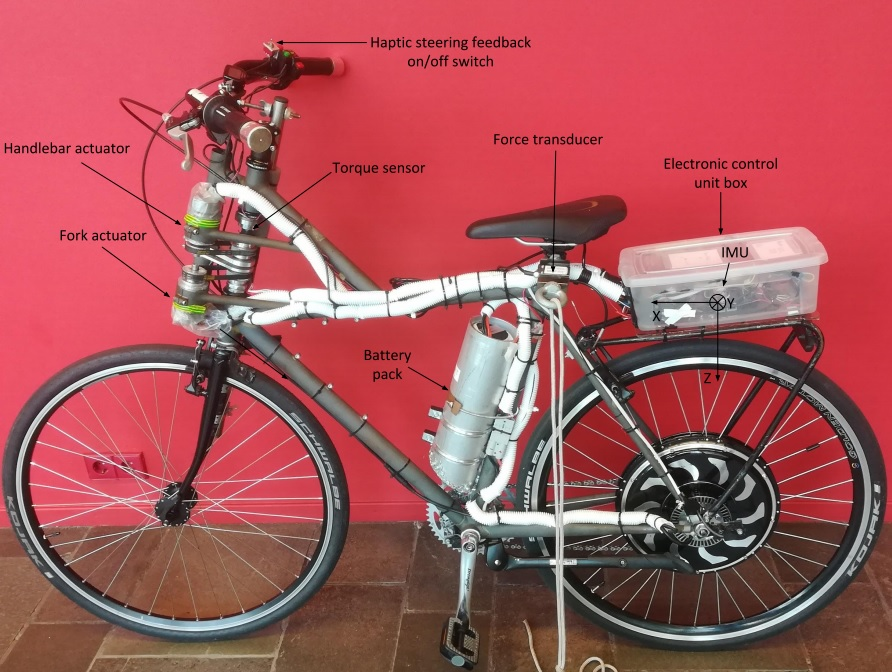
\includegraphics [width=0.8\textwidth]{images/steerbywirebicycle.jpg}
\caption{Prototype of the steer-by-wire bicycle with steering and handlebar actuators, sensors, digital controller and custom made battery pack.}
\label{steerbywireprototype}
\end{figure}

\subsection{Description of steer-by-wire controller} 

To minimize the difference between the handlebar angle $\theta$ and the fork angle $\delta$, tracking control has been implemented. In this way, the steer-by-wire system should behave like an ordinary, mechanically steered bicycle, when the rider applies a steer torque at the handlebar. Two proportional-differential PD-controllers are implemented in order to provide an action-reaction torque $T_{PDH}$ to the handlebar and $T_{PDF}$ to the fork assembly. Angular velocity $\dot{\theta}$ and  $\dot{\delta}$ are estimated by taking the time derivative of angular position $\theta$ and $\delta$ respectively, for a fixed time interval of 1 ms. The double PD-configuration can also be used to manipulate the steer feedback torque independent of the tracking performance. The double PD-controller is of the following form:


\begin{equation}
T_{PDF}=K_{PF}(\theta-\delta)+K_{DF}(\dot{\theta}-\dot{\delta}),
\label{handlebar-controller}
\end{equation}
\begin{equation}
T_{PDH}=K_{PH}(\theta-\delta)+K_{DH}(\dot{\theta}-\dot{\delta})
\label{fork-controller}
\end{equation}

with proportional gains $K_{PH}$, $K_{PF}$ and differential gains $K_{DH}$, $K_{DF}$ respectively. The torque $T_{PDH}$ is applied at the upper servomotor, and the torque $T_{PDF}$ at the lower servomotor. By setting $T_{PDH}$ to zero a steering configuration is created where the rider feels no reaction torque from the steering assembly (feedback "off"), without majorly affecting tracking error performance. The current controller configuration performs with high level of accuracy up to 3 Hz, the tracking error is kept below 3 degrees. However, in certain conditions non-linear effects of the servomotors and tires might create a delay in the control loop effecting the tracking error and realism of the haptic steering feel.


\subsection{Experimental Procedure}

Twenty healthy subjects volunteered in this study. To assure safety all subjects were requested to wear protective equipment in the shape of a standards-approved bike helmet, knee and elbow pads. All participants gave informed consent according to the guidelines of the human research ethics committee of Delft University of Technology. All subjects were healthy and reported that they did not experience any kind of pain or injury in the year before the experiments. The mean weight of all subjects was selected to be close to the European population \cite{walpole2012weight}.

Each experiment trial consisted of four different speeds (i.e., 2.6, 3.7, 4.5, 5.6 \si{\meter\per s}). Two individual trials were performed in total for every speed. In the first trial steering feedback was enabled, whereas in the second trial steering feedback was disabled. Every trial had a duration of approximately 60 seconds. All experiments were performed across Heertjeslaan cycling path of TU Delft, the subjects were requested to ride the steer-by-wire bicycle in all aforementioned speeds while being laterally perturbed. An additional bicycle was used from the experiment coordinator to cycle next to the instrumented steer-by-wire bicycle and perturb the subject, see figure \ref{lateralexperiment}. A set-up which allowed both push and pulls was initially tested but the pushes were subject to inconsistencies. After inspecting the data of the pilot runs, it was observed that unilateral disturbances did not affect the predictability of the perturbation, as the response of the rider was similar. For this reason the unilateral approach was chosen. Nevertheless, to avoid any feedforward control behaviour (e.g., seeing the coordinator preparing to pull the rope) all subjects were asked to keep their focus on the road ahead. 

\begin{figure}[htbp]
\centering
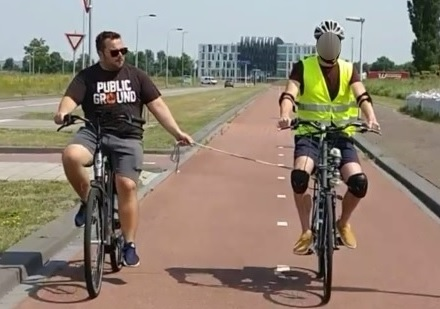
\includegraphics [width=0.8\textwidth]{images/lateralexperiment.jpg}
\caption{Experimental trial performed across Heertjeslaan cycling path of TU Delft; Experiment coordinator cycling next to steer-by-wire bicycle while pulling laterally the subject with a rope.}
\label{lateralexperiment}
\end{figure}

\subsection{System Identification}

In order to remove the effects of unwanted disturbances and noise, the  measured steering angle and estimated  roll angle signals were filtered through a finite impulse response (FIR) model. The impulse response function is defined as the function \(h(\tau)\) which when convoluted with external input \(w(t)\) results in the output \(y(t)\). The output data either represents \(y(t)=\phi(t)\) corresponding to \(h_\phi(\tau)\) or \(y(t)=\delta(t)\) corresponding to \(h_\delta(\tau)\). In discrete time the convolution can be approximated by the following equation:
\begin{equation}
\label{eq:1}
y(t)=\sum_{\tau=0}^{T-1} h(\tau) w(t-\tau)\Delta \tau + v(t)
\end{equation}
where \(T\) is the time length of the impulse function, which  is equal to 3.08 seconds as the oscillations die out after that point and \(v(t)\) the remnant which is caused by unwanted disturbances.
Equation \ref{eq:1} is rewritten in matrix form as follows:
\begin{equation}
\label{eq:2}
y=Wh+v
\end{equation}
where W is the matrix containing time shifted versions of the the input signal.
\begin{equation}
W=\begin{bmatrix} {w(0)} & {0} & {0} & {\dots} & {0} \\ {w(1)} & {w(0)} & {0} & {\dots} & {0} \\ {w(2)} & {w(1)} & {w(0)} & {\dots} & {0} \\ {\vdots} & {\vdots} & {\vdots} & {\ddots} & {0} \\ {w(N-1)} & {w(N-2)} & {w(N-3)} & {\dots} & {w(N-T)}\end{bmatrix}
\end{equation}
Since equation \ref{eq:2} is linear in the parameters (the coefficients of h) there exists a unique solution that can be found through the least squares method.
\begin{equation}
\hat{h}=\left(W^{T} W\right)^{-1} W^{T} y
\end{equation}
Having an estimate of the IRF, the input signal is convoluted with (\(\hat{h}\)) in order to produce  an estimate of the output (\(\hat{y}\))  without the noise. The estimated responses are further smoothed using a eight-order Butterworth filter with cutoff frequency of 10 Hz.


\subsection{Comparison Metrics}
In order to correctly assess if there is a statistically significant difference between the two conditions, three metrics are defined. The first one is the  Power Spectral Centroid (PSC) of measured angle (\(\delta\)) defined as 
\begin{equation}
(PSC_x , PSC_y) =\Bigg( \frac{\sum_{n=1}^{N} f(n) S_\delta(n)}{\sum_{n=1}^{N} S_\delta(n)},\frac{\sum_{n=1}^{N}  S_
\delta(n)^2}{\sum_{n=1}^{N} S_\delta(n)}\Bigg)
\end{equation}

where N is the number of samples lower than 5 Hz and \(S_\delta(f)\) the power spectral density of the signal. This metric gives an indication of the frequency  which most of the power in the signal is centered around. Higher value of \(PSC_x\) will indicate more oscillatory behaviour for the steering response and can be used as a metric of control effort.

The variance accounted for (VAF) is  used to assess  the quality of the fit of the FIR model output. The runs which scored lower than 60\% were removed from further analysis as it was deemed that the model did not sufficiently capture the characteristics of the raw signal. The VAF between  \(\hat{h}_\phi^{off}\) and \(\hat{h}_\phi^{on}\) is also used as a metric of similarity for the roll angle response. In that case VAF is defined as :
\begin{equation}
\mathrm{VAF}_{\phi}=\left(1-\frac{\operatorname{var}\left(\hat{h}_\phi^{off}-\hat{h}_\phi^{on}\right)}{\operatorname{var}\left(\hat{h}_\phi^{off}\right)}\right) \cdot 100 \%
\label{eq:3}
\end{equation}


Finally as a third test, the relative delay between the steering angle IRFs of the two conditions is estimated by finding the lag value of maximum cross-correlation between the signals.

\section{Results}

An independent 2-sample  t-test was conducted to compare if there was significant difference (95 \% confidence interval) in steering effort between conditions for all speed levels, see figure \ref{fig:pscentroid}. For the low speed level ( \(2.6 \;\si{\meter\per s}\)) there was no significant difference in \(PSC_x\) for "feedback on" (M = 0.79, SD = 0.08) and "feedback off" (M = 0.76, SD = 0.10) conditions; t(38)=1.00, p=0.3222. For speed  \(3.7\; \si{\meter\per s}\) there was again no significant difference in the metric for "feedback on" (M = 0.92, SD = 0.11) and "feedback off" (M = 0.92, SD = 0.11); t(38)= -- 1.03, p=0.3075. For  \( 4.5 \;\si{\meter\per s}\) there was also no significant difference in the scores for "feedback on" (M = 0.98, SD = 0.14) and "feedback off" (M = 0.98, SD = 0.14); t(38)= -- 1.04, p=0.3062. And finally, for \( 5.6\; \si{\meter\per s}\) no significant difference was found in the \(PSC_x\) for "feedback on" (M = 1.1, SD = 0.16) and "feedback off" (M = 1.1, SD = 0.16) conditions; t(38)= -- 1.6, p=0.118. 

\begin{figure}[htbp]
\centering
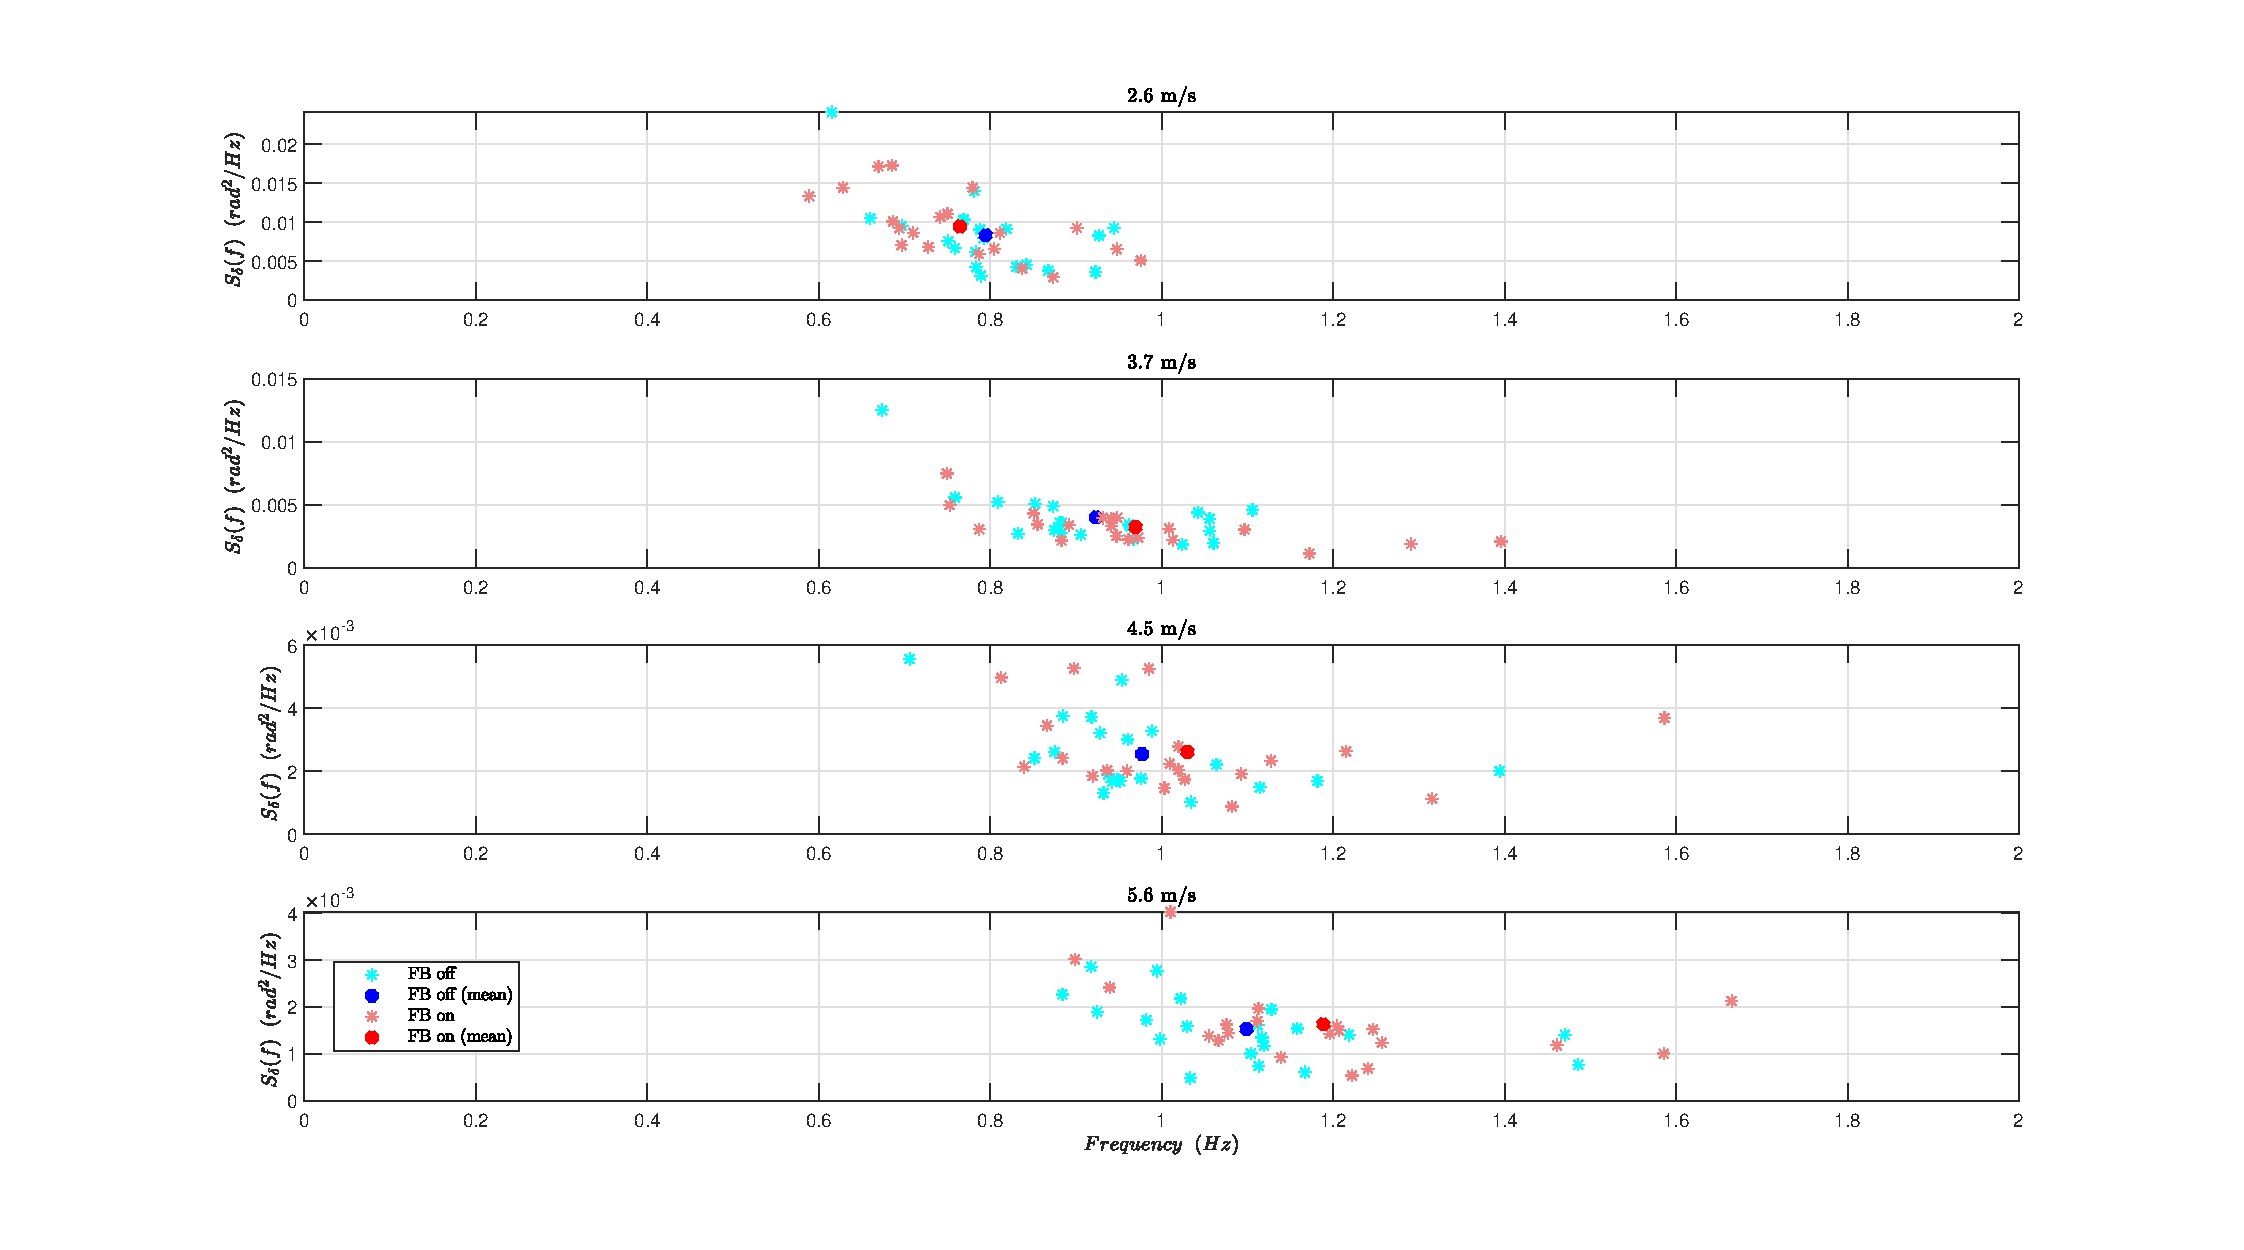
\includegraphics [width=1\textwidth]{images/PSC3.eps}
\caption{The x and y coordinate of the PSC used to determine the frequency where most of the power is concentrated.}
\label{fig:pscentroid}
\end{figure}

The impulse response function of the mean rider for steer angle (\(\delta\)) and roll angle (\(\phi\)) is shown in figure \ref{fig:irf}. The variance accounted for between roll angle impulse responses (see equation \ref{eq:3}) is averaged over all participants and displayed for all speed levels in figure \ref{fig:BoxPlots} (a). Similar roll angle response between "feedback on" and off indicated by higher \(\mathit{VAF}_\phi\) values suggests matching task performance.

\begin{figure}[htbp]
\centering
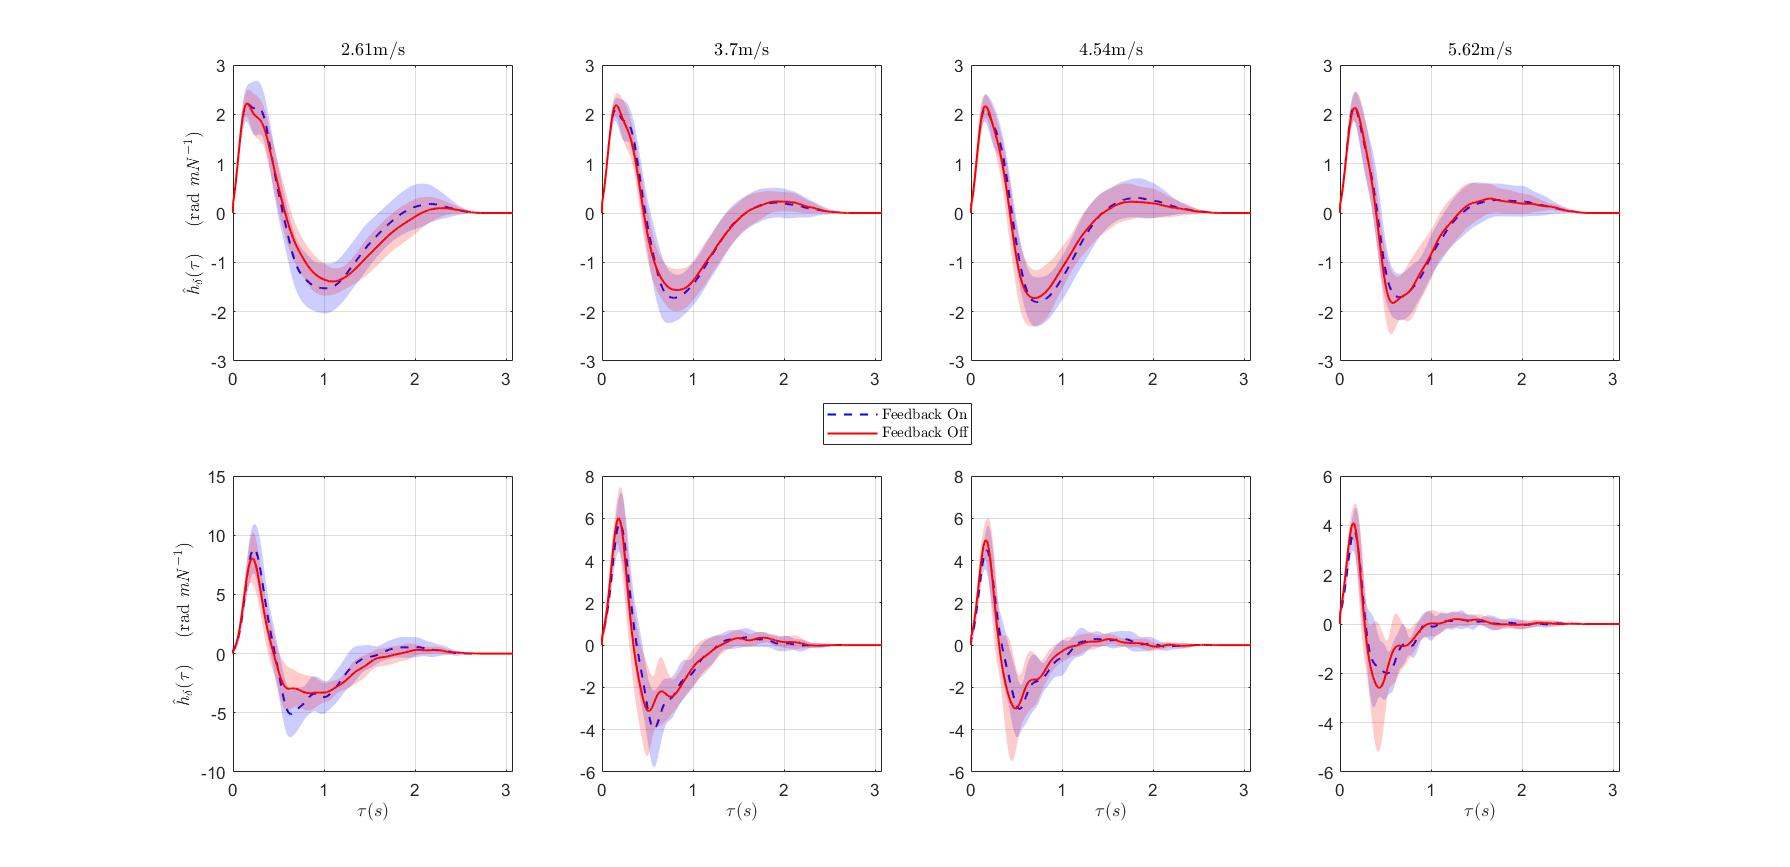
\includegraphics [width=1\textwidth]{images/meanIRF.jpg}
\caption{The impulse response function of the mean rider for steer angle (\(\delta\)) and roll angle (\(\phi\)). The shaded area represents the values within one standard deviation of the mean.}
\label{fig:irf}
\end{figure}

 In addition to the variance roll test an one-sample t-test was conducted to examine if there is any delay in the steering response between feedback on and off, see figure \ref{fig:BoxPlots} (b). For 2.6 m/s there was no significant deviation in the delay (M = -- 3, SD = 25.89) from zero mean; t(19)= -- 0.52, p=0.6103. However, for 3.7 m/s the delay (M = -- 20.65, SD = 25.93) was statistically significant; t(19)= -- 3.56, p=0.0021. Also for 4.5 m/s the mean of the delay (M = -- 23.5, SD = 20.88) was also significantly different than zero; t(19)= -- 5.03, p=0.0001. Lastly, for 5.6 m/s there was again significant difference in the delay (M = -- 19.15, SD = 18.19) from zero; t(19)= -- 4.71, p=0.0002.

% \begin{figure*}[h]
%  \centering
%  \subfigure[]{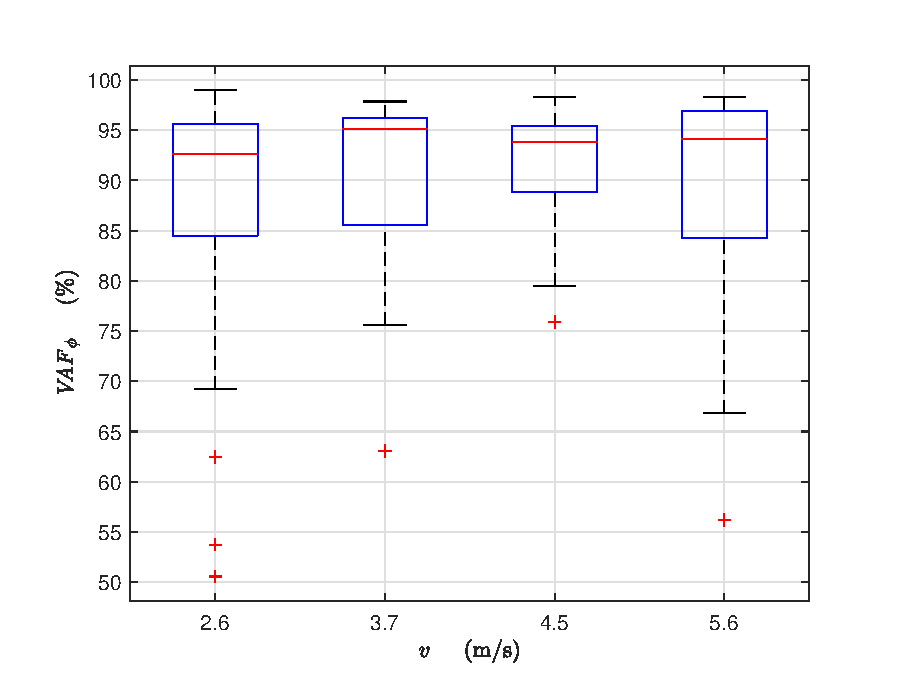
\includegraphics[width=0.61\textwidth]{images/vaf_phi.eps}}
% \subfigure[]{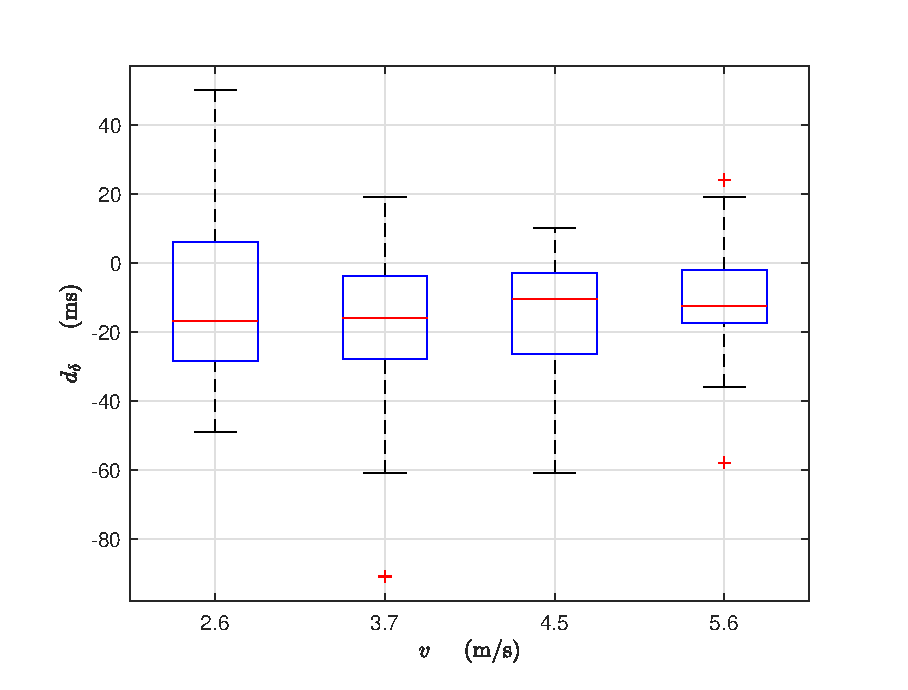
\includegraphics[width=0.61\textwidth]{images/delayBOX.eps}}
%  \caption{ a) Box plot of variance accounted for between roll angle impulse response functions for all speed levels. b) Box plot of the relative delay in the estimated steering angle response  between the two experimental conditions. Negative value means that the "feedback on" signal is delayed compared to the "feedback off".}
% \label{fig:BoxPlots}
% \end{figure*}

% \begin{figure}[h]
%     \centering
%     \begin{subfigure}{0.5\textwidth}
%         \centering
%         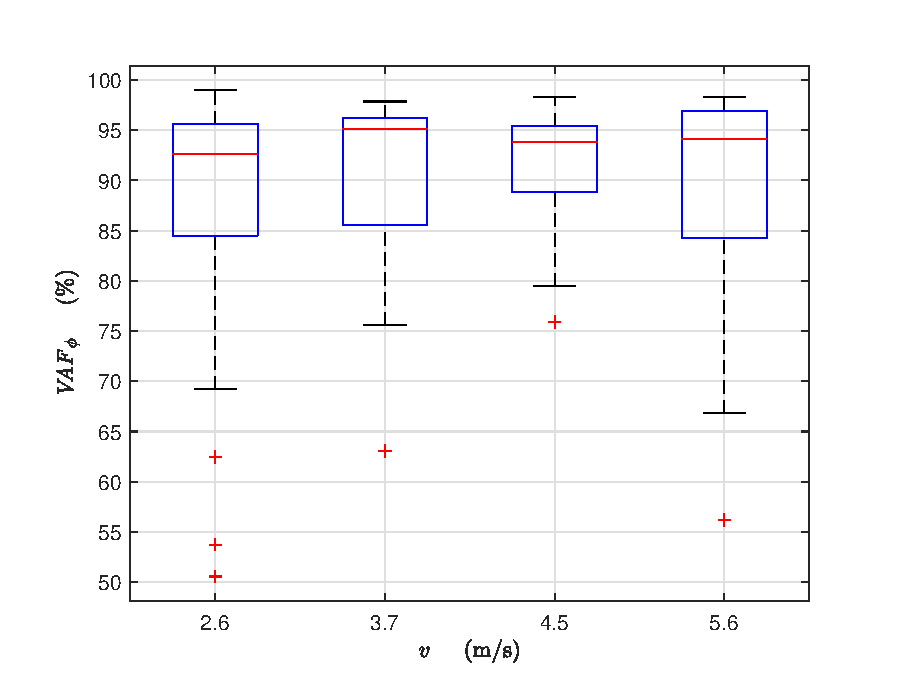
\includegraphics[width=.4\linewidth]{images/vaf_phi.eps}
%         \caption{}
%     \end{subfigure}
%     \begin{subfigure}{0.5\textwidth}
%         \centering
%         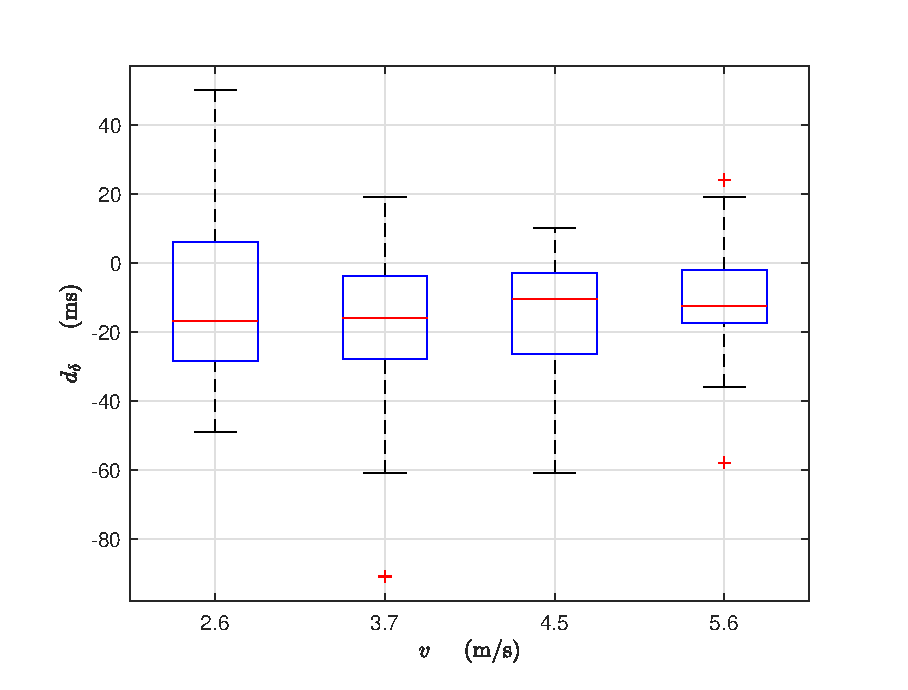
\includegraphics[width=.4\linewidth]{images/delayBOX.eps}
%         \caption{}            
%     \end{subfigure}
%     \caption{ a) Box plot of variance accounted for between roll angle impulse response functions for all speed levels. b) Box plot of the relative delay in the estimated steering angle response  between the two experimental conditions. Negative value means that the "feedback on" signal is delayed compared to the "feedback off".}
%     \label{fig:BoxPlots}
% \end{figure}

\begin{figure}[h]
    \centering{
     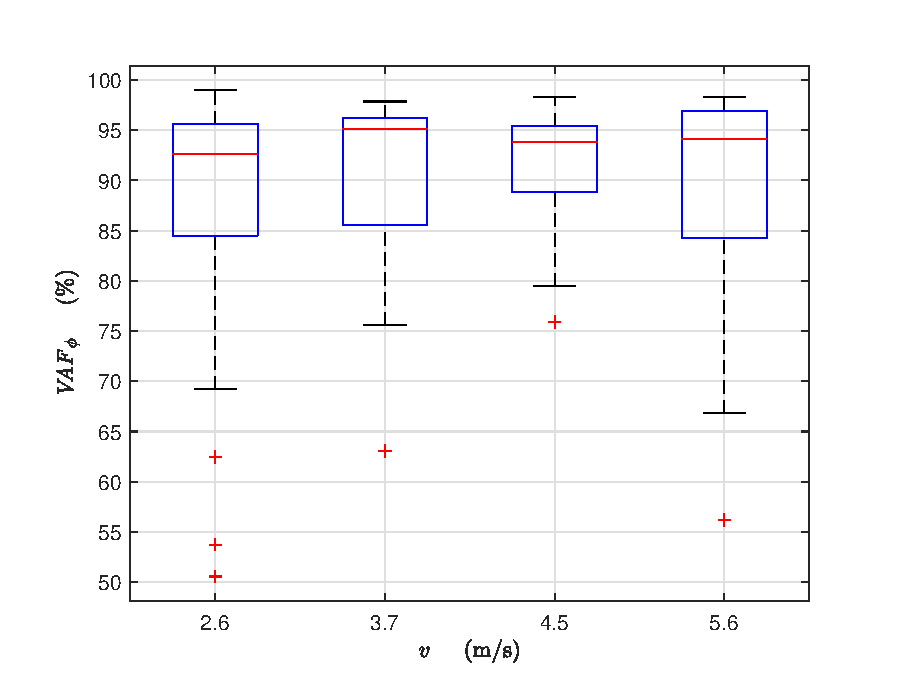
\includegraphics[width=.4\linewidth]{images/vaf_phi.eps}
     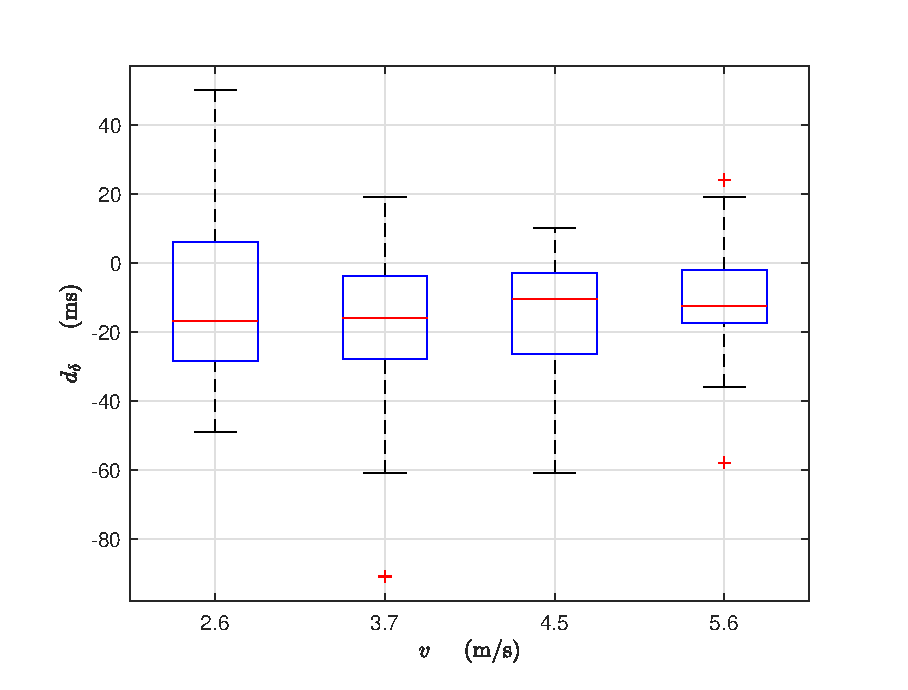
\includegraphics[width=.4\linewidth]{images/delayBOX.eps}

    }
    \caption{ a) Box plot of variance accounted for between roll angle impulse response functions for all speed levels. b) Box plot of the relative delay in the estimated steering angle response  between the two experimental conditions. Negative value means that the "feedback on" signal is delayed compared to the "feedback off".}
    \label{fig:BoxPlots}
\end{figure}

\section{Discussion and Conclusions}

From the aforementioned results it is suggested  that the effects of haptic feedback are minimal to non-existent for the roll stabilization task. Neither performance (see figure \ref{fig:BoxPlots} (a)) or steering effort was affected by the removal of haptic steering feedback. Balance performance among conditions was comparatively consistent  (see figure \ref{fig:BoxPlots} (a)). However, in the unstable speed region the variance and the number of outliers were higher. For steering effort the null hypothesis that the $\mathit{PSC}_x$ metric came from independent random samples with equal means and equal variances failed to be rejected for all speed levels. This does not undoubtedly prove that the samples came from the same population, howbeit it gives a strong indication towards that fact. On the other hand, for the "feedback on"  the steering response was delayed (\(\approx 18\; \si{ms}\) see figure \ref{fig:BoxPlots} (b)) in comparison to the "feedback off". This might be due to the fact that the handlebars are more inert due to the additional steering feedback. 

The lateral pull disturbances can be translated into a lean torque in the direction of forward speed and a steer torque in the direction of the steering axis. This means that any dynamic effects that influences these torques must be examined. The performance of the steer-by-wire controller was examined by numerical simulation and subjective measurements. All subjects reported that they felt like riding a mechanically steered bicycle, no adaptation period was required before the experiments. During the experiments very little motion of the upper body was evident and steer control was expected to be the main mechanism for bicycle balance \cite{moore2011rider}. Thus, we assume that the intristic and reflexives responses of the upperbody do not affect the validity of these results.

Physiologically there are two ways in which proprioception works in order to give the rider information regarding the state of the front assembly. First are the muscle spindles which by detecting changes in velocity and position of the shoulder joint give the rider an estimation of the steering angle and steering rate of the handlebars. Second are the Golgi tendon organs which work as force feedback sensors. The sensory information provided by the latter sensor is what this experiment tried to invalidate. In the feedback on case, information from the ground reaction torque of the front tire is transferred through the handlebars to the sensory receptors of the rider arms and is used for further state estimation. In the feedback off case the steering feedback information is lost. 

Despite the change in the dynamics of the upper handlebar the response of the rider is almost identical. Thereupon, we assume that the internal controller of the rider is either adaptive or is driven by some combination of torque or position control. In the case of torque control this would mean complete re-adaptation of feedback gains which would have resulted in some kind of adaptation period for the  participants when they swapped steering configurations. Although, no adaptation period was needed for any of the participants. Alternatively, in the case of position control steer angle increments are feed-through an inverse model of the steering assembly to produce the necessary forcing element. In this case, switching between configurations, would mean re-adaptation of the internal model of the handlebar assembly. This is much more plausible as it mainly concerns tuning of the internal perception of handlebar inertia which can happen instantaneously. To reveal if the later assumption is true an additional study  that models the rider as position and torque controller will be conducted. The identified parameters of the former and later controller might lead into further insights regarding the conclusions of this study. 

\newpage



\vfill{All data and supplemental material related to this article is available online at \url{https://doi.org/10.5281/zenodo.3365351} (Dialynas et al., 2019)}. 

% \references{report}


  







\chapter{Rider control identification in bicycling under lateral perturbations using a gray box approach} \label{hapticFB}

\section{Introduction}

Balancing a bicycle in motion is an acquired skill which is poorly understood. From the first appearance of the modern bicycle in the late 1880s until now, dynamic models of uncontrolled bicycles have provided fundamental insight into bicycle stability in relation to speed and geometry\cite{meijaard2007linearized, kooijman2011bicycle}. Further research into human control is needed to design safer bicycles and explore the potential of new safety systems.  In depth-analysis of the rider sensory dynamics  including delays and thresholds are necessary to probe the dynamics of the rider-bicycle balance control mechanism.

Research in the field of cybernetics started in the 1950s to advance aircraft technology and understand pilot control. \citet{mcruer1959human} were one of the first who tried to model the human operator as a servo system element with  time delay. The so called "McRuer cross over model" was later extended to the "McRuer precision model" which accounted for low frequency neuromuscular lags \cite{mcruer1967manual}.  Results showed that the human tries to adapt its control strategy in order to achieve a first order integrator open loop transfer function  near the systems cross-over frequency. Among the first researchers who focused in the manual control of bicycles were \citet{van1970influence}. They used a stationary bicycle simulator and system identification techniques to identify the rider control at a constant speed of 4.2 m/s . They described the rider as a proportional– integral–derivative (PID) position controller with delay. Although, their results are questionable since the bicycle simulator had no visual display and the obtained controller has not been experimentally validated. Roland et al. \cite{roland1971massing, roland1973computer} developed a bicycle stability and path following torque controller. The controller consisted of an inner and outer loop responsible for roll stabilization and lateral tracking, respectively. The stabilization controller was described as a PID with delay, whereas the tracking controller as a simple proportional controller. Results showed adequate performance but validation of the simulated responses has not been examined yet. \citet{weir1973manual} developed a cross-over model for Sharp's  \cite{sharp1971stability} motorcycle model in order to identify the transfer functions of the various control input–output relations. He concluded that steer torque response to lean angle error is the easiest way to balance a motorcycle in motion. \citet{eaton1975man} later conducted experiments to validate both the theoretical motorcycle model of  \citet{sharp1971stability} and rider model of \citet{weir1973manual} . Despite the fact that, he excluded the lean torque and used only the inner roll stabilization loop as a control input, results showed that low uncertainty was present in the estimated control parameters and low discrepancy in the fitting of the steer torque responses. \citet{hess2012modeling} attempted to introduce a task independent handling qualities metric for bicycle control. For this reason, he developed a model with five gains, two fixed second-order filters, and a preview time. \citet{schwab2013} recently tried to model the bicycle rider using lateral force perturbation experiments. A rider control model applying steering torque at the handlebars has been developed to explore the potential feedback of sensory cues during the bicycle balancing task. The identified rider control parameters, after model reduction, stabilize the system and mimic realistic rider control behavior.

The majority of aforementioned modeling approaches represent the rider as a torque controller and incorporate system delays. Albeit, the selected delays do not attribute directly to the physical response time of the visual, vestibular and proprioceptive system. Furthermore, none of these models include any type of internal model control (IMC) as frequently happens in most of human motor control studies \cite{francis1976internal, garcia1982internal, wolpert1995internal, gillespie2016human}. Consequently, the ability of humans to adapt and altered steering dynamics even when feedback is intermittent or delayed has never been examined.  Aside from that, the effect of haptic steering feedback in the balancing of bicycling has never been examined parametrically . Therefore, the role of the sensory receptors and in particular of the proprioception muscle splindes (position feedback) and golgi tendon organs (force feedback) during the riding process remains a black box .

The aim of this study is to evaluate the performance of three different control approaches with increased complexity and also examine the effect of  handlebar torque feedback during the steering and balancing task. The performance of all models are compared with the experimentally derived non-parametric finite impulse responses (FIR's) of  \citet{dialynaseffect}. Two metrics are used to assess the performance of the three controllers and to analyse the impact of torque feedback on rider control. The covariance coefficient (CV) of the estimated controller parameters is used as a measure of uncertainty, whereas the variance accounted (VAF) as a measure of fitting between the simulated and actual responses.

% In the lateral perturbation experiments conducted for two experimental conditions (torque feedback on and off), a statistical significant difference for control effort and task performance  could not be discerned. This indicated that the  rider despite the reduced feedback and changed bicycle dynamics managed to compensate and produce similar outputs. For this reason, a gray box analysis is conducted in this work to get further insights on what and why might have led to the findings derived in \cite{dialynaseffect}.

\section{Methods}
  In this work system identification techniques are employed to develop a rider control model andn  investigate the effectiveness of torque feedback via a gray box analysis . The ultimate goal is to formulate a model that best simulates bicycle rider balance behavior. This is done by comparing the parametric  results of  three torque feedback level conditions. In the first, the torque feedback loop is part of the rider control model. In the second, it is removed by setting its corresponding gain value to zero. In the third, the effectiveness of torque feedback is reduced by altering the plant dynamics and creating a steering configuration where the forces that would naturally transfer from the front wheel contact point to the handlebars are canceled, similar to how the haptics off case was implemented in the experimental condition \cite{dialynaseffect}. The full methodology is summarized in the list below:
\begin{enumerate}
    \item Black box identification : the procedure described in \cite{dialynaseffect} is followed to produce impulse response functions (IRFs), through the use of a FIR model, for steering angle \ensuremath{\delta}, roll angle \ensuremath{\phi}, yaw angle \ensuremath{\psi} and steer torque  \ensuremath{T_\delta}. This is done in order to extract the linear relationship between disturbance and measurements effectively filtering intrasubject variability. In the case of \ensuremath{T_\delta} instead of considering the whole bicycle rider closed loop system as a black box, the bicycle rider open loop is chosen with input the disturbance \ensuremath{w} and output the control input \ensuremath{T_\delta} (see \cref{fig:blackbox}).
    \item The produced IRFs \ensuremath{h^\delta(\tau)}, \ensuremath{h^\phi(\tau)}, \ensuremath{h^\psi(\tau)}, \ensuremath{h^{T_\delta}(\tau)} are filtered using zero-phase low pass filter with a cutoff frequency of 10 \si{\hertz}.
    \item The complete dataset is split into a training and a validation subdataset. The IRFs are averaged over each subdataset's participants in order to produce 2 mean rider responses. The variance accounted for \ensuremath{\mathit{VAF}}, between each individual's  response and the mean rider's, is calculated. The rider with the highest  \ensuremath{\mathit{VAF}} for all outputs  across all speed levels  is chosen as the median rider of each dataset. All further parameter estimation is conducted on the response of the median rider of the training dataset. Analysis is chosen to be conducted on the median rider since intersubject variability was low as is shown in \cite{dialynaseffect}.
    \item The IRFs of the median rider are convolved with the measured disturbances of each run to produce the non-parametric output \ensuremath{y_\delta(t)}, \ensuremath{y_\phi(t)}, \ensuremath{y_\psi(t)}, \ensuremath{y_{T_\delta}(t)}.
    \item Zero Delay Model gray box identification: A gray box model  is fit to the measured lateral force and the filtered response of the FIR
    model for each run. This is repeated for three conditions. In the first, the control process dynamics approximate a normal bicycle and will be referred to as haptic feedback on (haptics on), while  the rider has the torque feedback loop connected. In the second, the control process dynamics approximate again a normal bicycle, but the internal torque feedback loop of the rider is severed. In the third condition the steering dynamics change to that of steer-by-wire. This means that the coupling between roll and steer dynamics is modified. The rider is only receiving feedback due to the inertia of the handlebar and motor drive components. This condition is referred to haptic feedback off (haptics off).
    \item Variable Delay Model gray box identification: The model is updated with time delays. The model  is fit to the measured lateral force and the filtered response of the FIR model for each run. This is repeated for the three conditions described above. 
    \item  Variable Delay Reafferent Optimal Prediction (VDROP) Model gray box identification: The gray box model is updated with a delay compensation algorithm. The model is fit to the measured lateral force and the filtered response of the FIR model for each run. This is repeated for the three conditions described above.
    \item Assessment on the importance of torque feedback is made based on the the normalized covariance of the identified gray box parameters and the change of \ensuremath{\mathit{VAF}}  in the lateral force to steer angle fit between conditions.
    \item Assessment on the delay compensation strategy used is made based on the fitting performance across gray box models. Additionally the predictor is compared with a more conventional approach found in motor control literature. Finally the predictive capability of the VDROP model is tested by comparing its results with the median rider of the validation dataset. 

\end{enumerate}
\begin{figure}[h]
    \centering{
     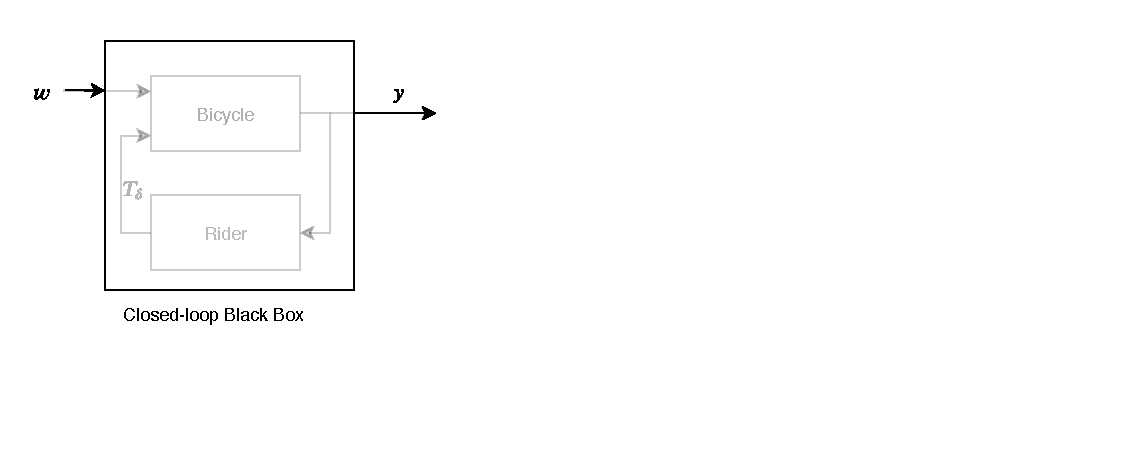
\includegraphics[width=.49\linewidth,trim={0 2cm 8.5cm 0.3cm},clip]{images/blackbox3.pdf}
     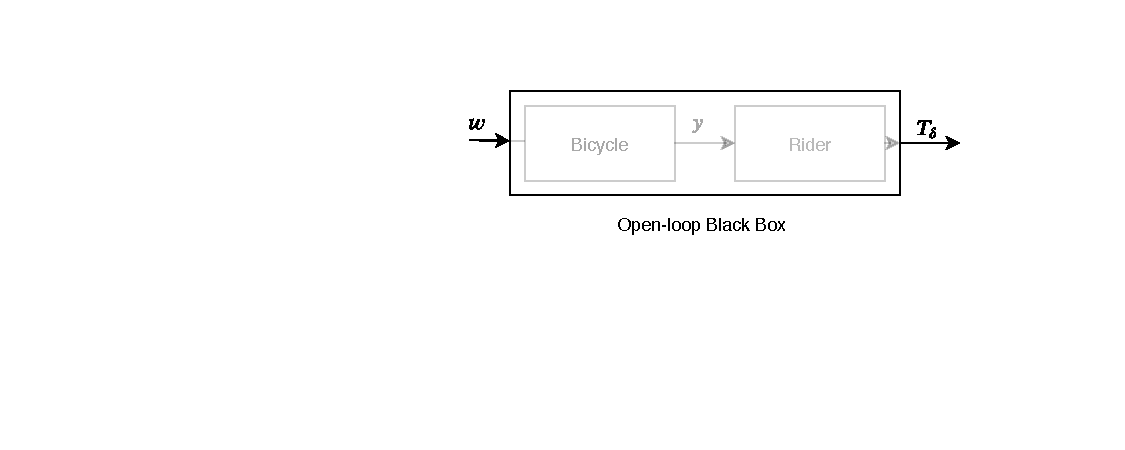
\includegraphics[width=.49\linewidth,trim={7.5cm 2cm 0 0.4cm},clip]{images/blackbox2.pdf}

    }
    \caption{The bicycle rider closed loop black box system used in the FIR model for extracting the linear relationship between disturbance \ensuremath{w} and outputs \ensuremath{\phi,\delta,\psi} (left). The bicycle rider open loop black box system used in the FIR model for extracting the linear relationship between disturbance \ensuremath{w} and control input \ensuremath{T_\delta} (right).  }
    \label{fig:blackbox}
\end{figure}



\subsection{Bicycle Model}
The bicycle model used is the so called Whipple-Carvalho model the dynamics of which have been expressed in a set of linearized equations by \citet{meijaard2007linearized}. In the original model three assumptions are made. The first is that the rider is rigidly attached in the saddle with the mass of the arms and legs acting as a point. Secondly, the contact between tire and ground is modeled as a non slipping rolling point contact meaning that the wheels can rotate without lateral slip. Lastly it is assumed that the total energy of the system is preserved. The resulting non-holonomic mechanical model has three velocity degrees of freedom, the forward speed, the rear frame roll rate \ensuremath{\dot{\phi}} and the steering rate \ensuremath{\dot{\delta}}.
\begin{figure}[ht]
    \centering
    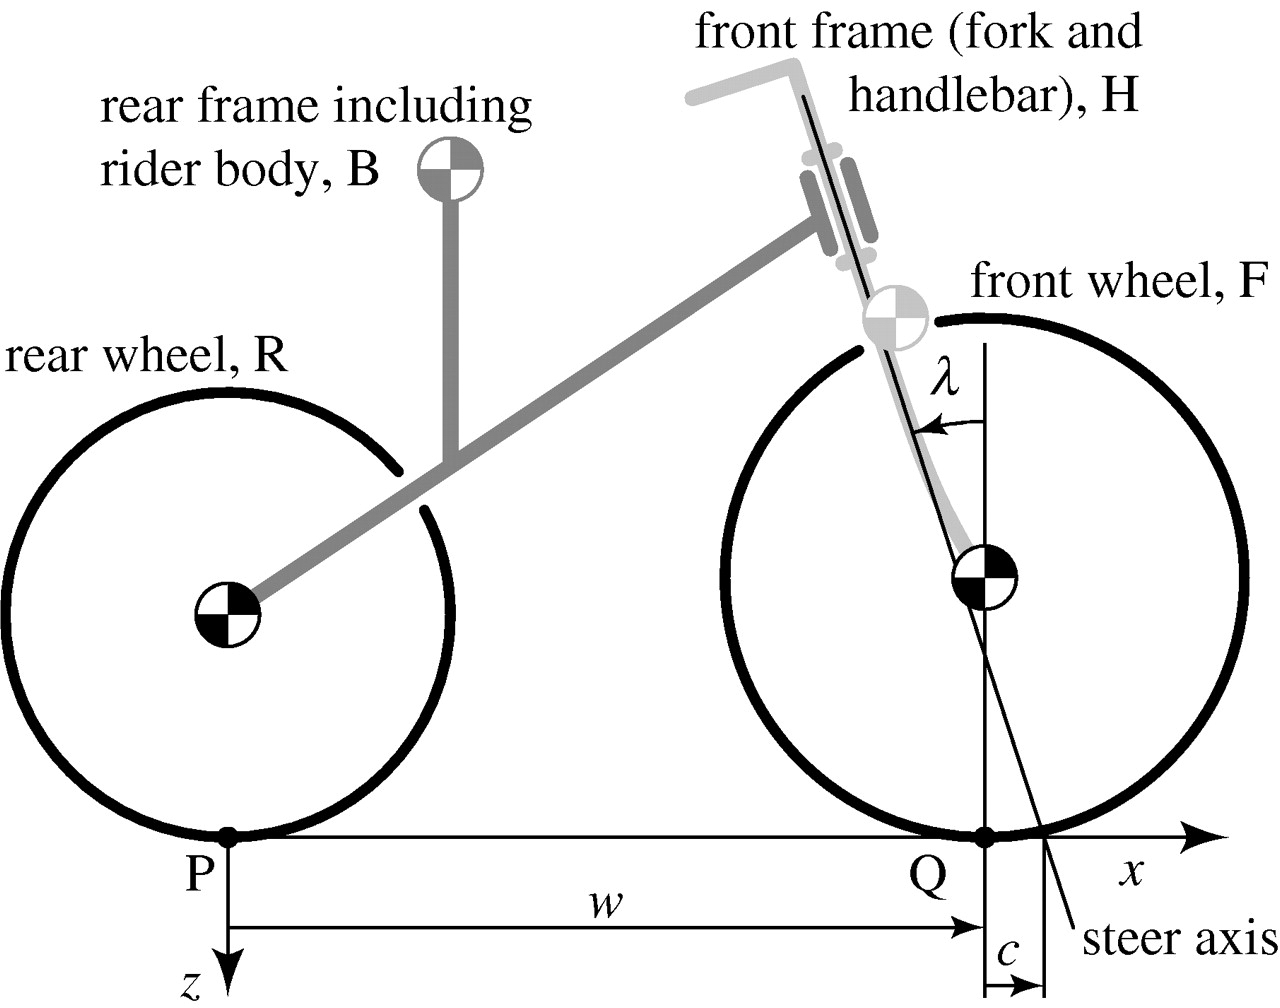
\includegraphics[scale=0.3]{images/figure3_1.png}
    \caption{ The Whipple-Carvalho bicycle model consists of four rigid bodies: rear wheel R, rear frame B, front frame H and front wheel F connected via hinges. The center of mass locations are expressed relative to the x - and z -coordinates shown (with origin at P and y pointing towards the reader). The other parameters shown are the steer axis tilt \ensuremath{\lambda}, wheelbase \ensuremath{w} and trail \ensuremath{c}. The model at its most expanded form is described by 25 parameters.\cite{meijaard2007linearized}}
    \label{fig:figure2}
\end{figure}
The lateral motion is described by  two coupled second order differential equations given by \cref{eq:paper1}.
\begin{equation}
    \mathbf{M} \ddot{q}+v \mathbf{C}_{1} \dot{q}+\left[g \mathbf{K}_{0}+v^{2} \mathbf{K}_{2}\right] \mathbf{q}=\mathbf{f}
    \label{eq:paper1}
\end{equation}

where \ensuremath{\mathbf{q}} is a vector containing the roll and steer angles, \ensuremath{\mathbf{f}} is a vector containing the roll and steer torques, \ensuremath{g} is the gravitational acceleration and \ensuremath{\mathbf{M},\;v\mathbf{C}_{1},\;g \mathbf{K}_{0}+v^{2} \mathbf{K}_{2}} are the "mass", "damping" and "stiffness" ratios in matrix form respectively. The entries in the constant coefficient matrices  \ensuremath{\mathbf{M},\mathbf{C}_{1}, \mathbf{K}_{0},  \mathbf{K}_{2}} are calculated from a set of 25 bicycle parameters related to inertial and design properties of the steer by wire bicycle (see \cref{tb:paper1}).

To determine the stability of the open loop system in a straight ahead motion the characteristic polynomial derived from
\begin{equation}
    \operatorname{det}\left(\mathbf{M} \lambda^{2}+v \mathbf{C}_{1} \lambda+g \mathbf{K}_{0}+v^{2} \mathbf{K}_{2}\right)=0
    \label{eq:paper2}
\end{equation}

is solved for a forward speed range from 0 to 10 \si{\meter\per\second} where \ensuremath{\lambda} are the eigenvalues of the system (see \cref{fig:paper2}). The two interesting eigenmodes defined by the locus plot are the weave and capsize. The weave corresponds to an oscillatory mode as can be seen by the existence of imaginary parts and represents a motion in which the bicycle sways about its heading. The oscillatory motions exponentially fades when forward speed is larger than 4.39 \si{\meter\per\second}. The capsize on the other hand has an eigenvector dominated by lean and leads to a gradual roll drift to infinity when the eigenvalue crosses the zero line around 6.67 \si{\meter\per\second}.
\begin{figure}[ht]
    \centering
    \captionsetup{justification=centering,margin=2cm}

    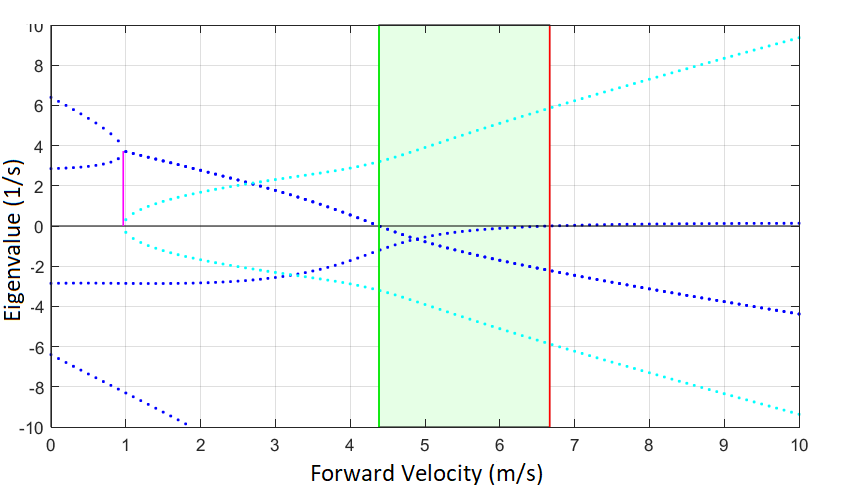
\includegraphics[scale=0.6]{images/root_locus_steerbywire.png}
    \caption{Root locus plot of the steer by wire bicycle. Dotted blue lines indicate the real part of the eigenvalues while dotted cyan show the imaginary part. The stable region corresponds to speeds  \ensuremath{4.39\lessapprox v \lessapprox 6.67\; \si{\meter\per\second}}}
    \label{fig:paper2}
\end{figure}
Since in the experimental setup the task could not be isolated to purely balance the equations are extended to include heading. Heading is defined as a linear combination of steer angle and steer rate as expressed by \citet{meijaard2007linearized} in \cref{eq:paper3}. 

\begin{equation}
    \dot{\psi}=\frac{v \delta+c \dot{\delta}}{w} \cos \lambda
    \label{eq:paper3}
    \end{equation}

When modeling the haptics off case of the steer-by-wire bicycle the dynamics of the plant need to change accordingly. In that configuration, the forcing steering input is directly proportional to steering acceleration, for this reason the second of the set of equations in \ref{eq:paper1} becomes :
\begin{align}
    M_{22}\ddot{\delta}+ M_{21}\ddot{\phi} + v{C_1}_{22}\dot{\delta} + v{C_1}_{21}\dot{\phi}+[g{K_0}_{22}+v^2{K_0}_{22}]\delta +[g{K_0}_{21}+v^2{K_0}_{21}]\delta &= T_{\delta} \\
    M_{22}\ddot{\delta} &= T_{\delta} \\
    I_{F_{xx}}\ddot{\delta} &= T_{\delta} 
\end{align}
where \ensuremath{I_{F_{xx}}} is the moment of inertia of the  decoupled handlebar assembly.
 
For control purposes \cref{eq:paper1} is expressed in state space form with state vector \ensuremath{\mathbf{x}=[\dot{\phi}, \dot{\delta}, \phi, \delta, \psi]^{T}}, forcing input \ensuremath{\mathbf{f}=T_{\delta}} and output equal to the full state. The  bike is assumed to be controlled only by a steering torque because according to both \citet{moore2012human} and \citet{weir1973manual}  the rear frame roll angle is mainly
 controlled by steering. 
 \begin{align}
    \dot{\mathbf{x}} &=\mathbf{A} \mathbf{x}+\mathbf{B} T_\delta + \mathbf{H}_d w
     \label{eq:bikeEOM1}\\
    \mathbf{y}&=\mathbf{C} \mathbf{x}+\mathbf{D} T_\delta
    \label{eq:bikeEOM2}
\end{align}

where matrices \ensuremath{A,B,C,D,H_d} are defined by:
\begin{align}
    \mathbf{A} &=\begin{bmatrix}
        -\mathbf{M}^{-1}v\mathbf{C}_{1} & -\mathbf{M}^{-1}(g \mathbf{K}_{0}+v^{2}\mathbf{K}_{2}) \\
        {\mathbf{I}_2}                    & {\mathbf{0}} \\  {\begin{matrix} {0} & { \frac{c\cdot cos\lambda}{w}}\end{matrix}} &  {\begin{matrix} 0 & { \frac{v \cdot cos\lambda}{w}}\end{matrix} } 
    \end{bmatrix} , \mathbf{B}=\left[ \begin{array}{c}{\mathbf{M}^{-1}} \\ {\mathbf{0}}\end{array}\right] \\
    \mathbf{C} &= {\mathbf{I}_5} , \mathbf{D}=\mathbf{0} \\
    \mathbf{H}_d &= \left[ \begin{array}{c}{\mathbf{M}^{-1}}{\begin{bmatrix} l_g \\ c_s\end{bmatrix} }  \\ {\mathbf{0}}\end{array}\right] 
\end{align}

\ensuremath{\mathbf{H}_d} is the matrix defining the dynamics of the lateral disturbance \ensuremath{w}. In this case the force application point was \ensuremath{l_g} distance from the ground. The constant \ensuremath{c_s} coefficient is due to the coupled roll to steer dynamics and is selected as a fraction of \ensuremath{w} similar to \citet{schwab2013}. This results in an additional  torque perturbation \ensuremath{T_\delta } in the handlebars.

\subsection{Rider Control Model}\label{subsec:rider_model}

 The complete high level overview of the model is shown in \cref{fig:paper3}. The output state of the bicycle is concatenated with the steering torque to produce the complete vector of sensory inflow. The measurements attributed to the vestibular, visual and proprioceptive system of the human body are delayed and fed into a prediction algorithm that uses an internal model of the process dynamics to forward the measurements in time. This is made possible by the use of the efference copy, which is an internal copy of an outflowing, movement-producing signal generated by the motor system. The controller  is just a pure gain block with free parameters to be estimated through gray box system identification. The final control forcing input is produced after passing through a transfer function simulating the neuromuscular dynamics.
\begin{figure}[ht]
    \centering
    \captionsetup{justification=centering,margin=2cm}

    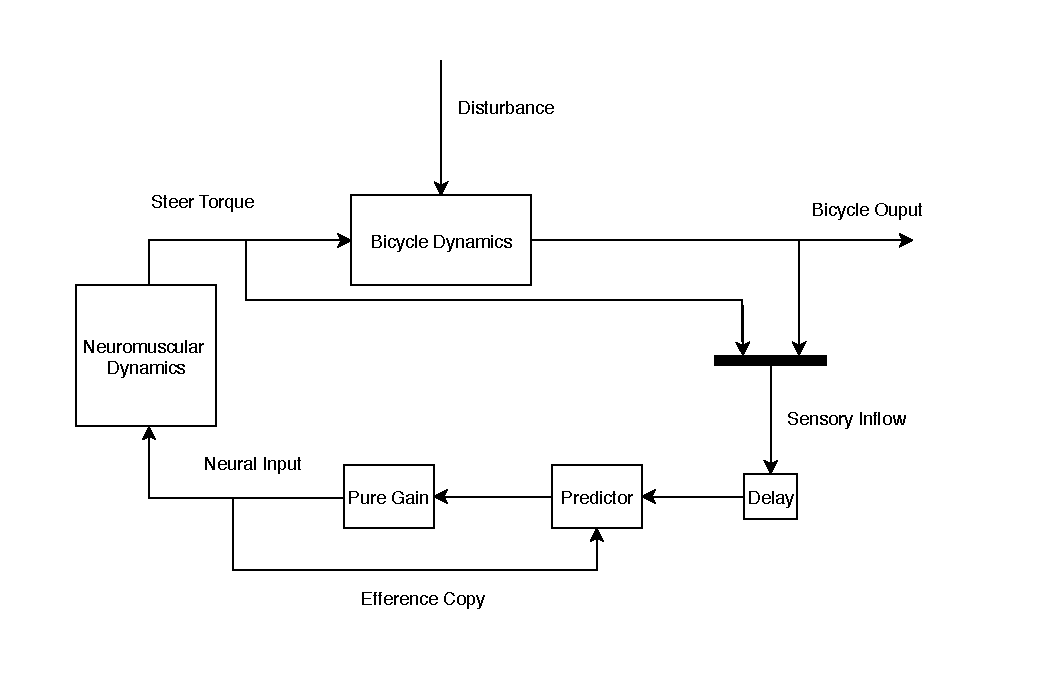
\includegraphics[scale=0.8]{images/high_level_block.pdf}
    \caption{Block diagram of the complete rider-bicycle model.} 
    \label{fig:paper3}
\end{figure}

The neuromuscular dynamics block works as a second order filter to simulate the limitations of the human response. In state space form this block is expressed by :

\begin{align}
\dot{x}_{nm} &= \begin{bmatrix}0 & 1 \\ -{\omega_c}^2 & -2\zeta{\omega_c}\end{bmatrix} \begin{bmatrix} T_\delta \\ \dot{T}_\delta\end{bmatrix} + \begin{bmatrix} 0 \\ {\omega_c}^2\end{bmatrix} a     \label{eq:gnmBLOCKA}    
    \\
y_{nm} &= \begin{bmatrix}1 & 0\end{bmatrix} \begin{bmatrix} T_\delta \\ \dot{T}_\delta\end{bmatrix}
    \label{eq:gnmBLOCKB}
\end{align}

where \ensuremath{\alpha} is the controller output representing the efferent neural signal, \ensuremath{\zeta} is the damping coefficient and \ensuremath{\omega_c} is the cutoff frequency. The latter two   parameters are chosen according to activation dynamics present in the shoulder joint \cite{happee2008posture}.

The steer angle \(\delta\) and steer rate \(\dot{\delta}\) feedback is attributed to the muscle spindles, while the torque feedback is made possible with the help of the golgi tendon organs. The roll and heading angle come from the visual system. Lastly the roll rate feedback is attributed to the vestibular system. 

The bicycle model of \cref{eq:bikeEOM} is combined with the neuromuscular dynamics block of \cref{eq:gnmBLOCKA,eq:gnmBLOCKB} to create a combined  plant with state \ensuremath{x=[\dot{\phi}, \dot{\delta}, \phi, \delta, \psi, T_\delta \dot{T}_\delta]^{T}} ,input \ensuremath{a} and \ensuremath{w} and output \ensuremath{y=[\dot{\phi}, \dot{\delta}, \phi, \delta, \psi, T_\delta]^{T}}. In order to make possible the implementation of the predictor which is discrete in nature the state space representation of the combined plant is discretized by zero order hold with a time step of 0.001 \si{\second}. The equivalent model block diagram is shown in \cref{fig:paper4}.

\subsubsection{The reafferent optimal predictor}
Many strategies to counter time delays have been proposed in literature. The most basic predictor is the Smith predictor, which has been explored in motor control research by \citet{miall1993cerebellum}. The Smith predictor compensates for time delays through the use of an internal forward model of the controlled dynamics and an internal model of the sensory delay pathways. The forward model works by utilizing an efferent signal of the control input while the comparison between prediction and measurement is trying to simulate the human's ability to distinguish between reafference and exafference.  Unfortunately the  most basic Smith predictor scheme does not work for unstable open loop systems \cite{smith1957closed}. In this work a modification to the normal Smith predictor scheme is suggested. In place of the forward model a discrete optimal predictor  (DOP) is used that forward simulates the amount of steps according to the model of sensory delay (see \cref{fig:delay_line}). This works like a resetting forward model that is updated every time step by the delayed state so the predictor loop does not become unstable. Because every sensory pathway has different time delays, the conventional DOP is adapted to work with variable time delay state input. This adapatation is illustrated with a simplified example in the block scheme of \cref{fig:VDROP_line}.  The DOP   without the Smith  correction can still work and has been implemented by \citet{van2001adaptive} for modeling stance control but it leads to predictions that do not contain any amount of the effect of the disturbance on the state. The block diagram of the predictor can be seen in \cref{fig:paper4}.

\begin{figure}[h!]
    \centering
    % \captionsetup{justification=centering,margin=2cm}

    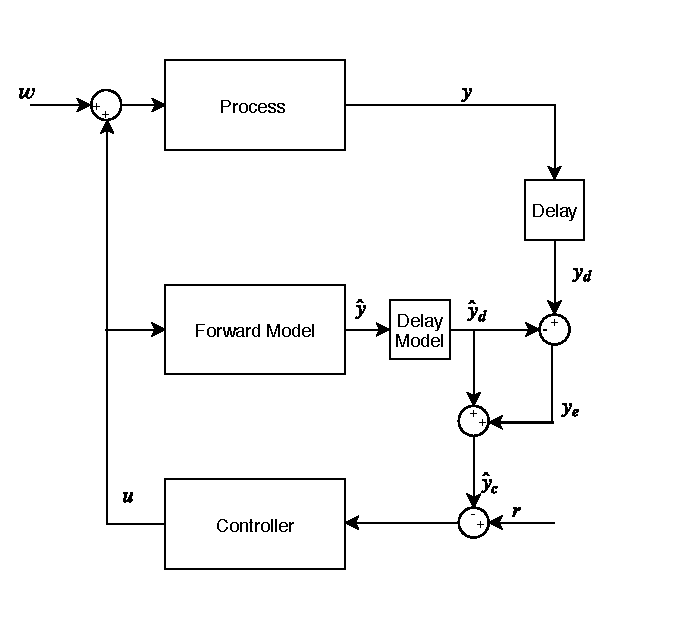
\includegraphics[width=0.6\linewidth]{images/smith.pdf}
    \caption{Block diagram of the basic Smith Predictor scheme. The Smith Predictor uses an internal  forward model  to predict the delay-free response \ensuremath{\hat{y}} of the process. It then compares this prediction  with the desired setpoint \ensuremath{r} to decide what adjustments are needed (control \ensuremath{u}). To prevent drifting and reject external disturbances, the Smith predictor also compares the actual process output with a prediction \ensuremath{\hat{y}_d} that takes the dead time into account. The gap \ensuremath{y_e=y_d-\hat{y}_d} is fed back  and contributes to the overall controller input. Note that \ensuremath{y_e} amounts to the perceived state mismatch delayed by the duration of dead time.}
    \label{fig:smith}
\end{figure}


\begin{figure}[h!]
    \centering
    % \captionsetup{justification=centering,margin=2cm}

    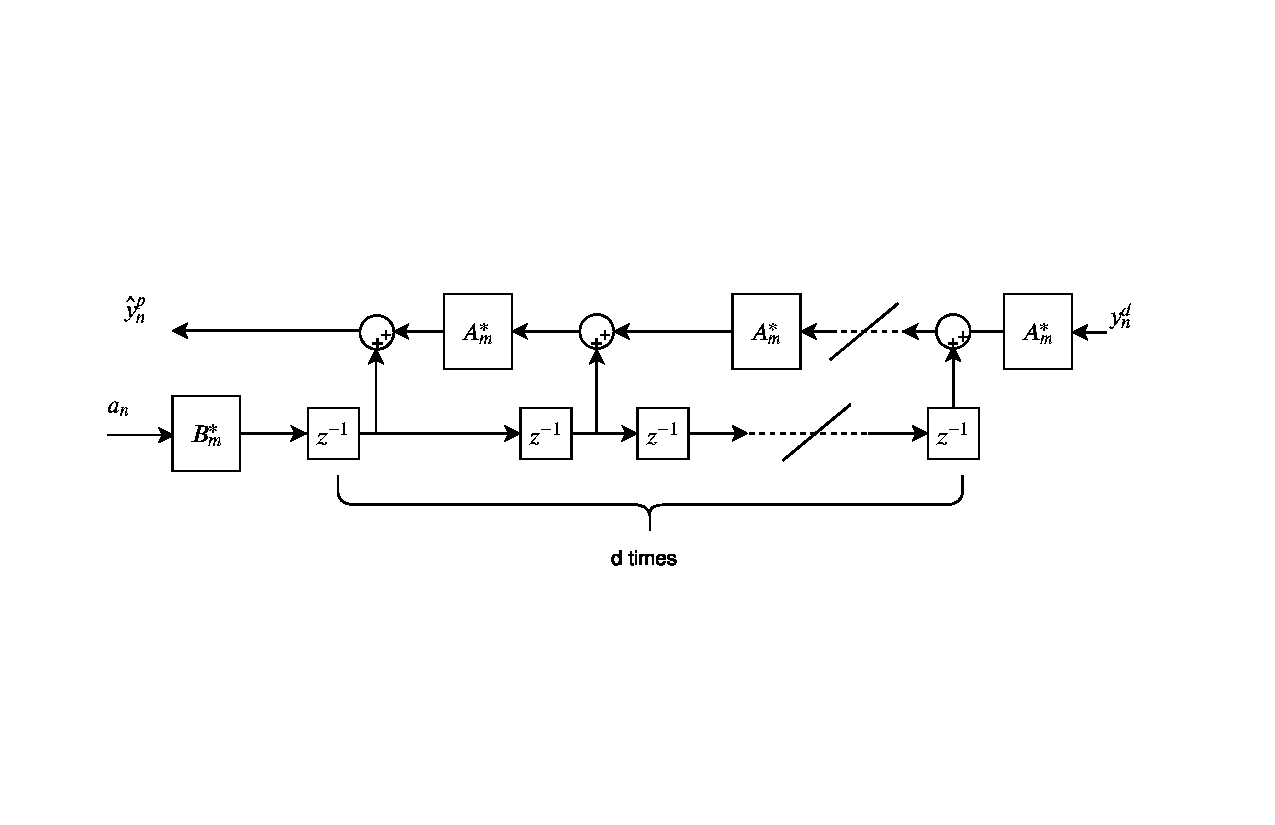
\includegraphics[width=\linewidth,trim={0 4.2cm 0 2cm},clip]{images/predictor_plots/tapped_delay.pdf}
    \caption{The discrete optimal predictor consists of a tapped delay line. The tapped delay line used in this work is a forward simulation of the discretised dynamics of the bicycle including neuromuscular dynamics. It uses the efference copy of the known previous control input \ensuremath{a_n}  and the delayed estimate \ensuremath{y^d_n}. \ensuremath{A^*_m} and \ensuremath{B^*_m} are the best available discrete approximation of these dynamics.}
    \label{fig:delay_line}
\end{figure}


\begin{figure}[h!]
    \centering
    % \captionsetup{justification=centering,margin=2cm}

    \rotatebox[origin=c]{90}{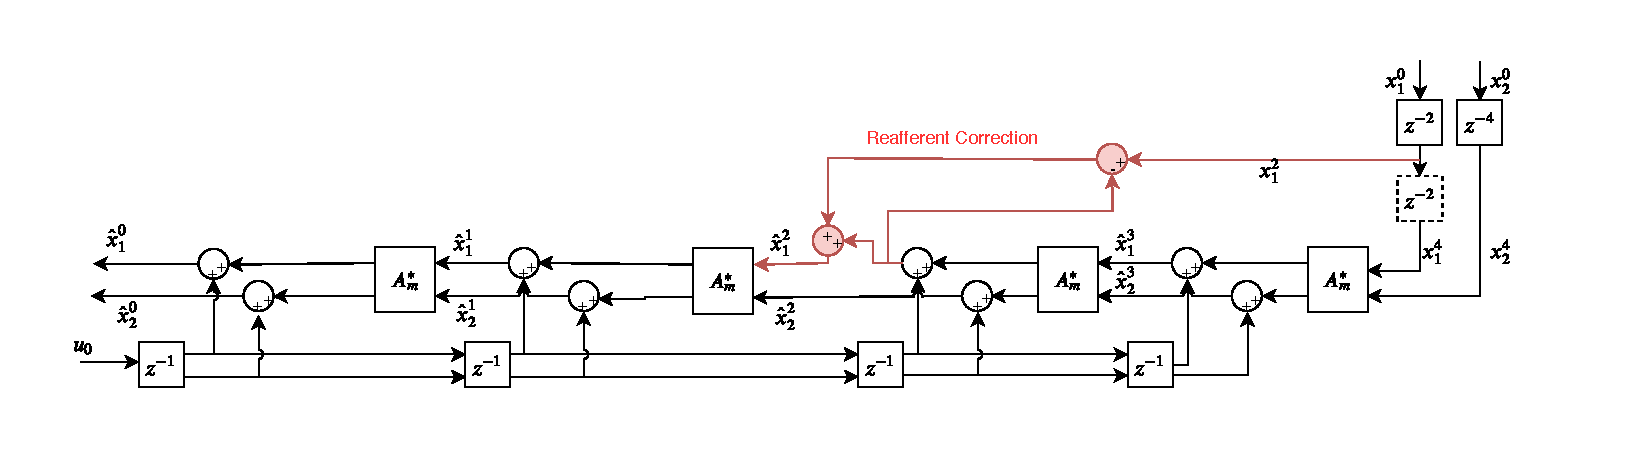
\includegraphics[scale=0.85]{images/VDROP_line.pdf}}
    \caption{Example that illustrates the adaptation necessary for the DOP to work with variable delay signals. States \ensuremath{x_1, x_2} are delayed according to their individual dead times. Since \ensuremath{x_1} has smaller delay value, it is further delayed through a model of the remaining delay to synchronize with \ensuremath{x_2}. The delayed state vector enters the tapped delay line until the point when the forward simulation produces an estimate of \ensuremath{x_1} that is concurrent with its measurement; in this case after 2 time steps. At that point the reafferent correction is performed shown  in red. After the correction the tapped delay line continues normally. Matrices \ensuremath{A^*_m} and \ensuremath{B^*_m} are the best available discrete approximation of the system dynamics, \ensuremath{u_0} is the current control input (efference copy).}
    \label{fig:VDROP_line}
\end{figure}
 \begin{figure}[ht]
    \centering
    % \captionsetup{justification=centering,margin=2cm}

    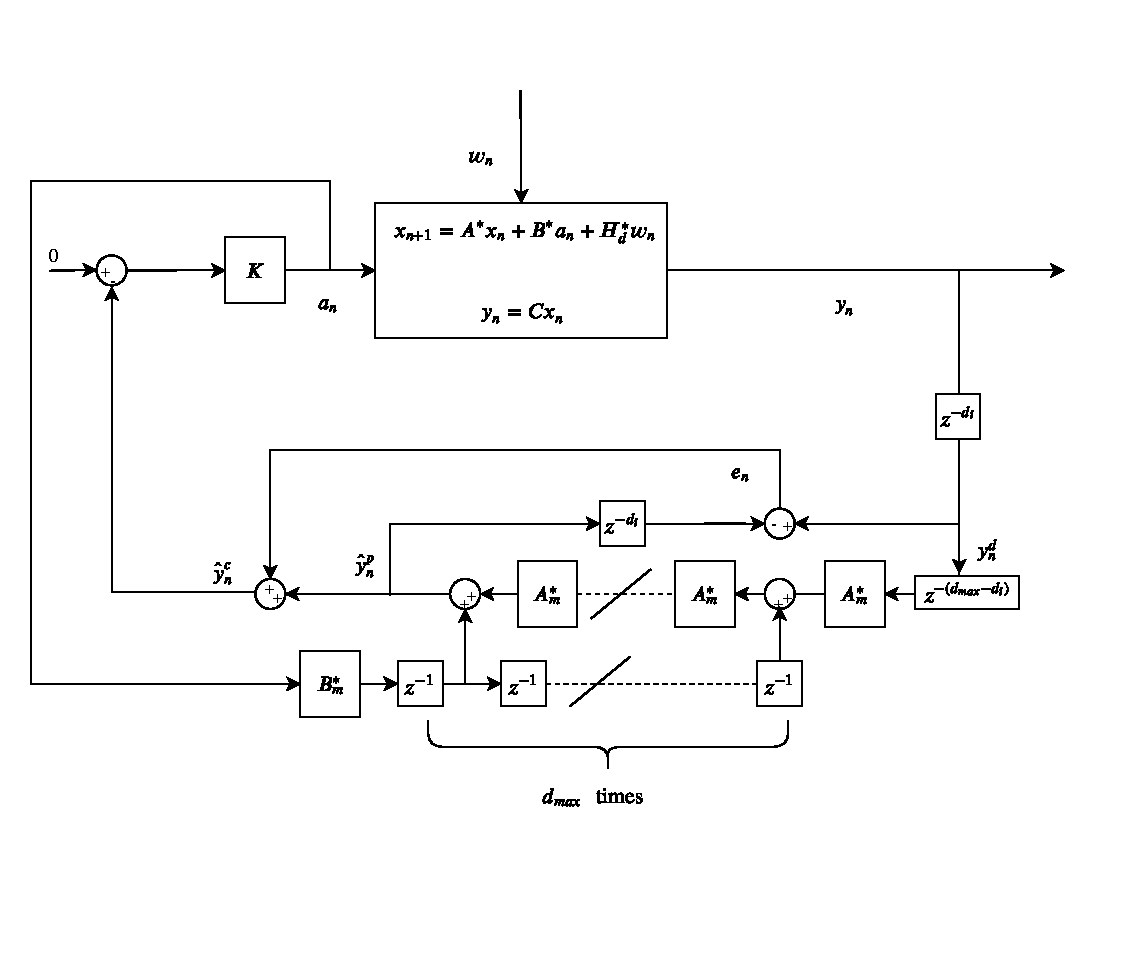
\includegraphics[width=\linewidth,trim={0 2.8cm 0 2cm},clip]{images/VDROP_block.pdf}
    \caption{Block diagram of the Variable Delay Reafferent Optimal Prediction Model. \ensuremath{A^*} ,\ensuremath{B^*}, \ensuremath{H_d^*} are the discretized matrices of the combined plant dynamics, \ensuremath{d_i} is the amount of delay in times steps per sensory channel and \ensuremath{d_{max}} the maximum value of those. Matrices \ensuremath{A_m^*} ,\ensuremath{B_m^*} express the dynamics of the internal model of the process. When the internal model is assumed to be perfect \ensuremath{A_m^*=A^*} and \ensuremath{B^*=B^*}. First the delayed measurements are all further delayed upto the maximum amount of delay among signals  in order to synchronize them.  The delayed output measurement  is forwarded in time (\ensuremath{d_{max}} times) in the tapped delay line to produce the first undelayed estimate of the output \ensuremath{\hat{y}^p}. When a less delayed measurement  of a certain state becomes available the tapped delay line  state register is updated with that measurement. This way the accumulation of forward simulation error is minimized. Output \ensuremath{\hat{y}^p} is again delayed through a model of the  internal time delay. The difference between this re-delayed prediction with the delayed measurements creates the error \ensuremath{e} which is added back to  \ensuremath{\hat{y}^p}  to create the final corrected prediction \ensuremath{\hat{y}^c}. }
    \label{fig:paper4}
\end{figure}

\subsection{Parameter Estimation }

In order to assess the effectiveness of the torque feedback loop, three models of incremental complexity are used. In the first the feedback pathways are fed into the controller without delays. In the second delays are added. The third one compensates for time delays by the use of the VDROP. The three models have the  controller gains as free parameters. More specifically, the gains are estimated by fitting the model output into the non-parametric data-set derived in \cite{dialynaseffect}.  The gains were estimated by minimization of the cost function 
\begin{equation}
    V_{N}(\boldsymbol{\theta})=\frac{1}{N} \mathlarger{\mathlarger{\mathlarger{\sum}}}_{k=1}^{N}\left[64\frac{\left(\hat{y}^{\delta}_k(\mathbf{\theta})-y^\delta_k\right)^{2}}{\underset{k}{\max} \left(y^\delta_k\right)^2}+11\frac{\left(\hat{y}^{\psi}_k(\mathbf{\theta})-y^\psi_k\right)^{2}}{\underset{k}{\max} \left(y^\psi_k\right)^2}+7\cdot10^{-6}\frac{\left(\hat{y}^{T_\delta}_k(\mathbf{\theta})\right)^2}{\underset{k}{\max} \left(y^{T_\delta}_k\right)^2}\right]
    \label{eq:cost}
    \end{equation}

where \ensuremath{\boldsymbol{\theta}} is a vector containing all the free parameters, \ensuremath{\hat{y}^{\delta}} and \ensuremath{\hat{y}^{\psi}} are the outputs of the simulation for the measured external disturbance \ensuremath{w} and the vector of parameters  \ensuremath{\boldsymbol{\theta}} for steer angle \ensuremath{\delta} and heading angle \ensuremath{\psi}  respectively, while \ensuremath{y^\delta} and \ensuremath{y^\psi} are the outputs of the non-parametric model.

The first two terms  of the cost function are trying to match the steering and heading  response of the parametric model with that one of the non-parametric model, while the third on minimizes the amount of input torque generated in order to produce the best possible fit while maintaining minimal control effort. The weights are chosen heuristically. For optimization the genetic algorithm with a fitness limit of 0.03 is first  used in order to produce a good starting parameter vector for gradient descend algorithm to take over, which finally finds the closest possible estimate of the global minimum. For the genetic algorithm a crossover fraction of 0.85  along with a population size 10 times the length of the parameter vector is used.

The gains attributed to the muscle spindle sensors (\ensuremath{K_\delta} and \ensuremath{K_{\dot{\delta}}}) are constrained to be only positive. The assumption is that they work like a delayed steering stiffness and damping. Additionally, the gains \ensuremath{K_\psi} and \ensuremath{K_\phi}  are constrained to fall under -250 and 250 \si{\kilogram\square\meter\per\second}.  When left unconstrained these parameters drive the whole gain vector to unrealistic values for insignificant amount of fitting performance increase (\ensuremath{<0.1\%}).

The impulse response function of the median rider is used. This is determined by taking the mean impulse response function of each measured output and finding the participant which had the highest variance accounted for between the individual response and the mean across all speed levels for all filtered outputs. Each system was identified for three different model conditions: 
\begin{enumerate}
    \item  6 feedback pathways including torque feedback
    \item  5 feedback pathways excluding torque feedback
    \item  6 feedback pathways including torque feedback but bicycle dynamics are switch to "haptics off".
\end{enumerate}
In the thrid condition the internal model used in the predictor is not updated to reflect the changed bicycle dynamics. This assumption is made due to the fact that no adaptation time  was noted in the experiments for any of the participants when switching the steering configurations so significant tuning of an internal model is not realistic. 

 As metric of model validity the variance accounted for between parametric and non-parametric output is used, defined as
\begin{equation}
\mathrm{VAF_d}(\boldsymbol{\theta})=1 -\sum_{k=1}^{n}\left(y^{d}(k)-\hat{y}^{d}(k, \boldsymbol{\theta})\right)^{2} / \sum_{k=1}^{n}\left(y^{d}(k)^{2}\right)
\label{eq:VAF}
\end{equation} 
where \ensuremath{d=\{\phi,\delta,\psi\}}. 

In order to assess the importance of the torque feedback, the uncertainty of each parameter is found. Parameters with the lowest uncertainty contribute more to the fit so they are deemed more important. To find the uncertainty the covariance matrix is estimated from :
\begin{align}
    \operatorname{cov}_{\hat{\theta}}  &=V_N(\boldsymbol{\hat{\theta}})\boldsymbol{H}(\boldsymbol{\hat{\theta}})^{-1}
    \label{fig:cov_mat}
    \\ \text{with} \;\;\;\;  \boldsymbol{H}(\boldsymbol{\hat{\theta}})&= \frac{\partial^{2} V_N}{\partial \theta_{i} \partial \theta_{j}}
\end{align}

where \ensuremath{\boldsymbol{\hat{\theta}}} is the closest estimate to the true parameter vector \ensuremath{\theta^*} that produces the true global minimum and \ensuremath{\boldsymbol{H}} is the hessian matrix numerically estimated by the gradient descend algorithm.  However, since bigger parameters are going to have naturally larger variances the diagonal values are normalized by the parameter value to produce the coefficient of variation.

\begin{equation}
    CV_{i}=\sqrt{\frac{\sigma^{2}_{\hat{\theta_i}}}{\hat{\theta}_i^2}}
    \end{equation}

    where \ensuremath{\sigma^{2}_{\hat{\theta_i}}} are the diagonal elements of \ensuremath{ \operatorname{cov}_{\hat{\theta}}}.
% As far as the delays are concerned for \ensuremath{\delta} and \ensuremath{\dot{\delta}} which are attributed to the muscle spindle sensors and for the torque feedback which is attributed to the golgi tendon organs  a delay of 25 \si{\milli\second} is chosen \cite{van2002identification,de2002adaptation}. For the feedback states attributed to visual feedback such as the roll angle \ensuremath{\phi} and yaw angle \ensuremath{\psi} a much greater delay of 200 \si{\milli\second} is chosen. Finally for  the vestibular roll rate feedback a delay of 50 \si{\milli\second} is implemented \cite{barnett2013vestibular}. 
% \cite{whipple1899stability}


\section{Results}


\subsection{Zero Delay Model}
The results of the zero delay model for the median rider are presented in \cref{tb:no_delay}. A \ensuremath{\mathit{VAF}} of over 90 \% is easily achieved for both steer angle and heading, while for roll the discrepancy is larger. A  look into how the model approximates the measured rider input and bicycle states for all forward speeds is seen in \cref{fig:zdm_fitA,fig:zdm_fitB}. Even in the ideal case with zero delays, the model inputs seems to lag behind the measured applied rider torque.

% \begin{figure}[!h]
%     % \centering
%     % \captionsetup{justification=centering,margin=2cm}
%     \makebox[\textwidth][c]{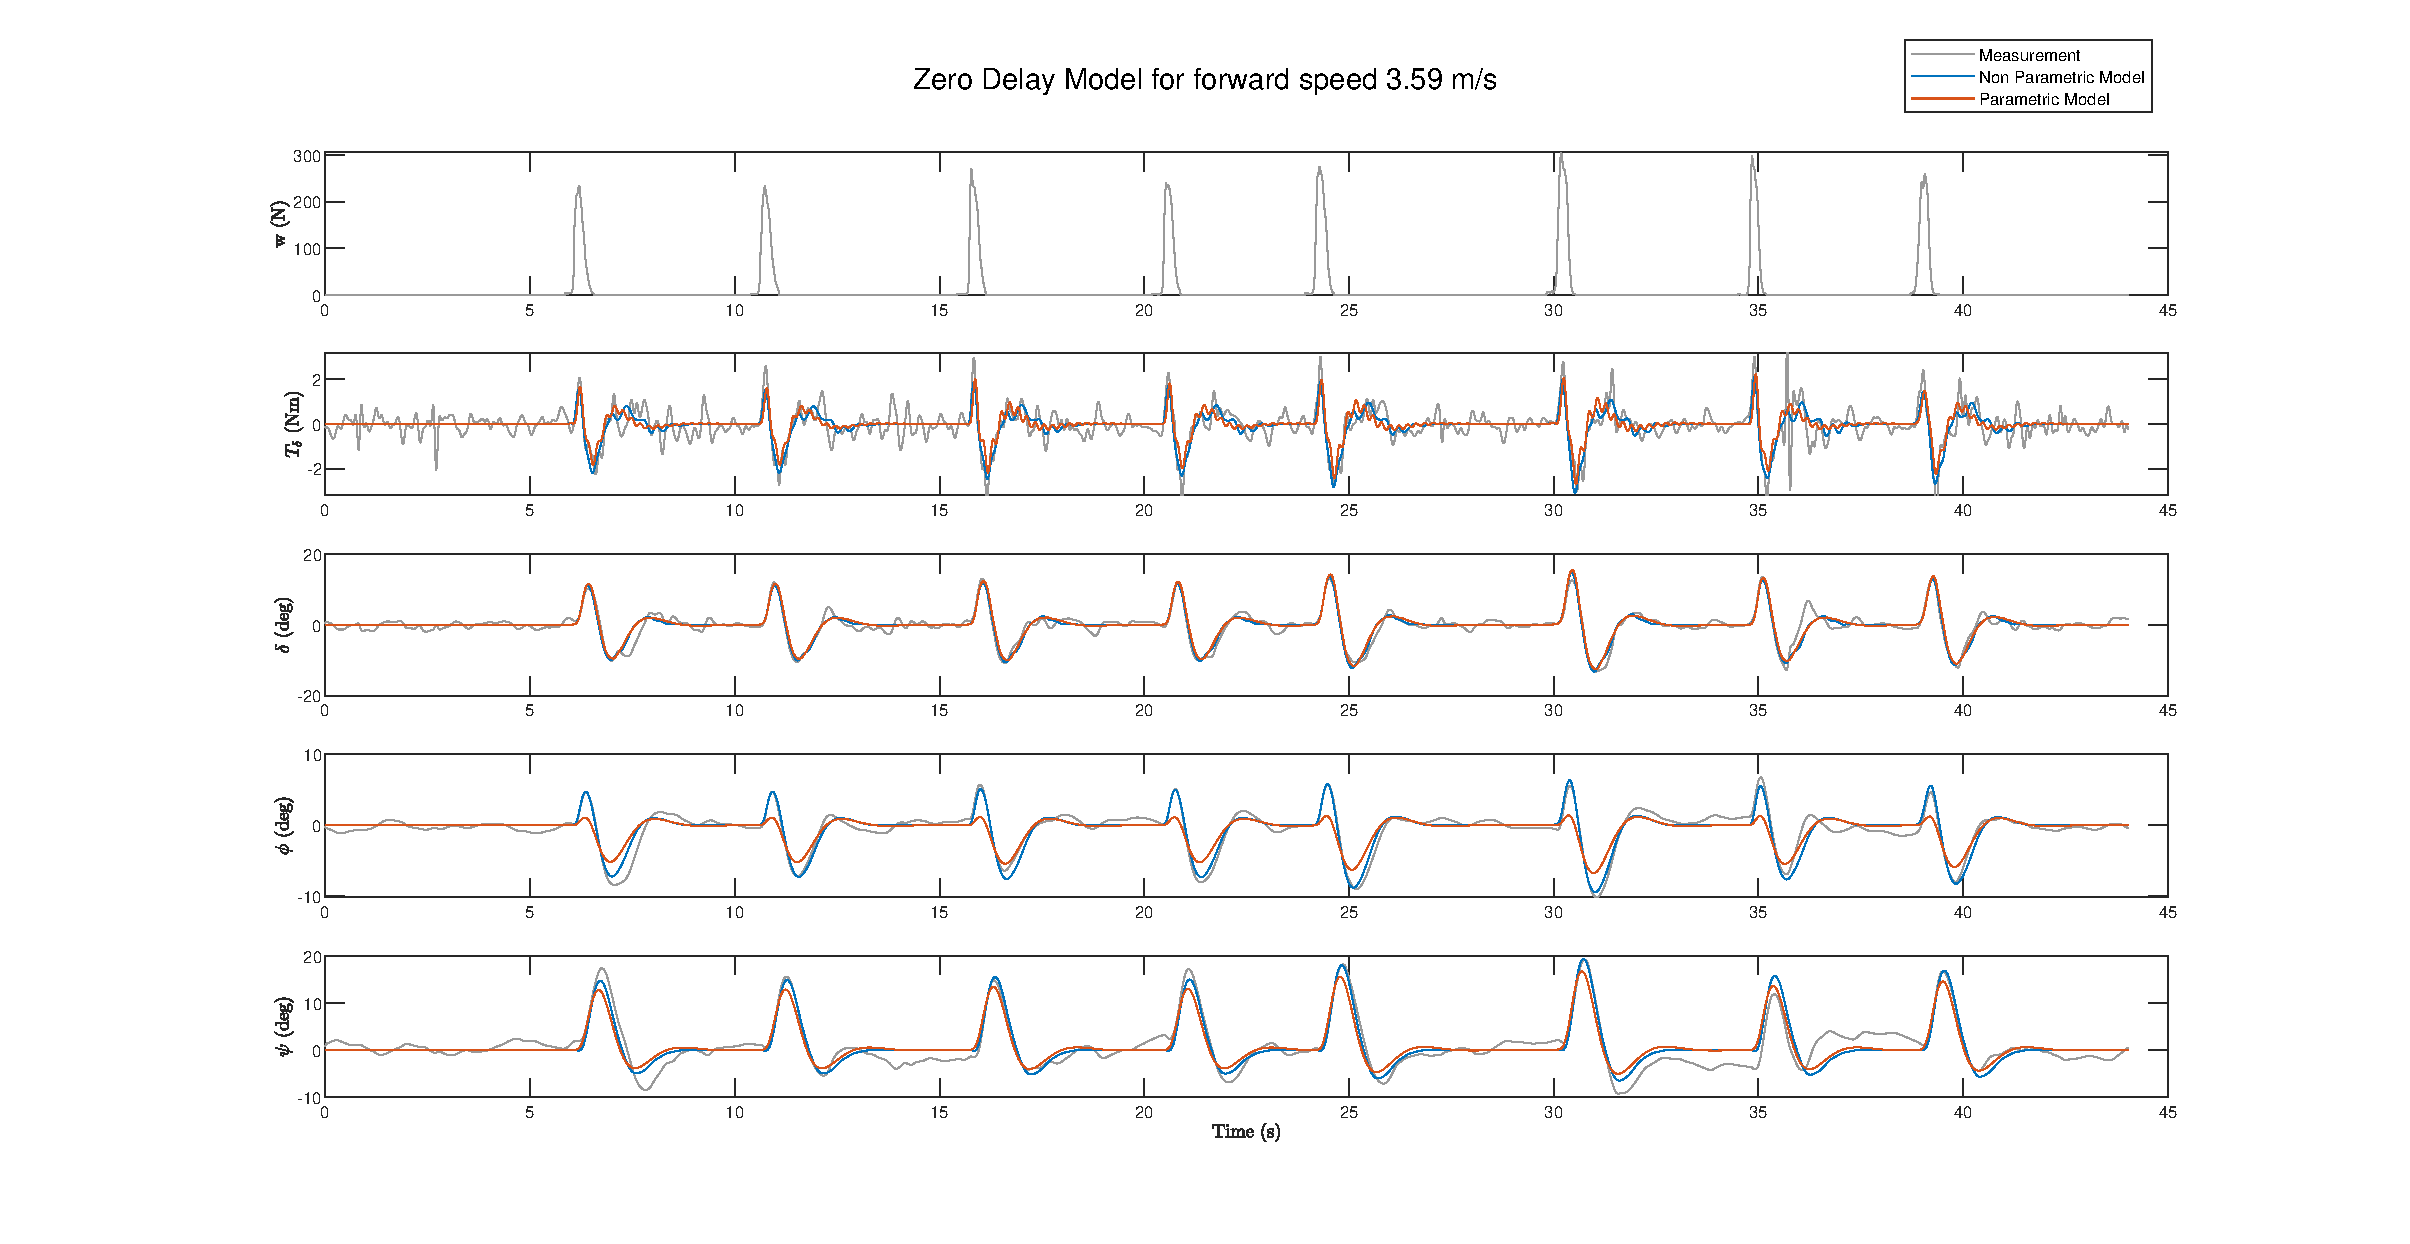
\includegraphics[width=1.4\textwidth]{images/no_delay_result1.eps}}
%     % 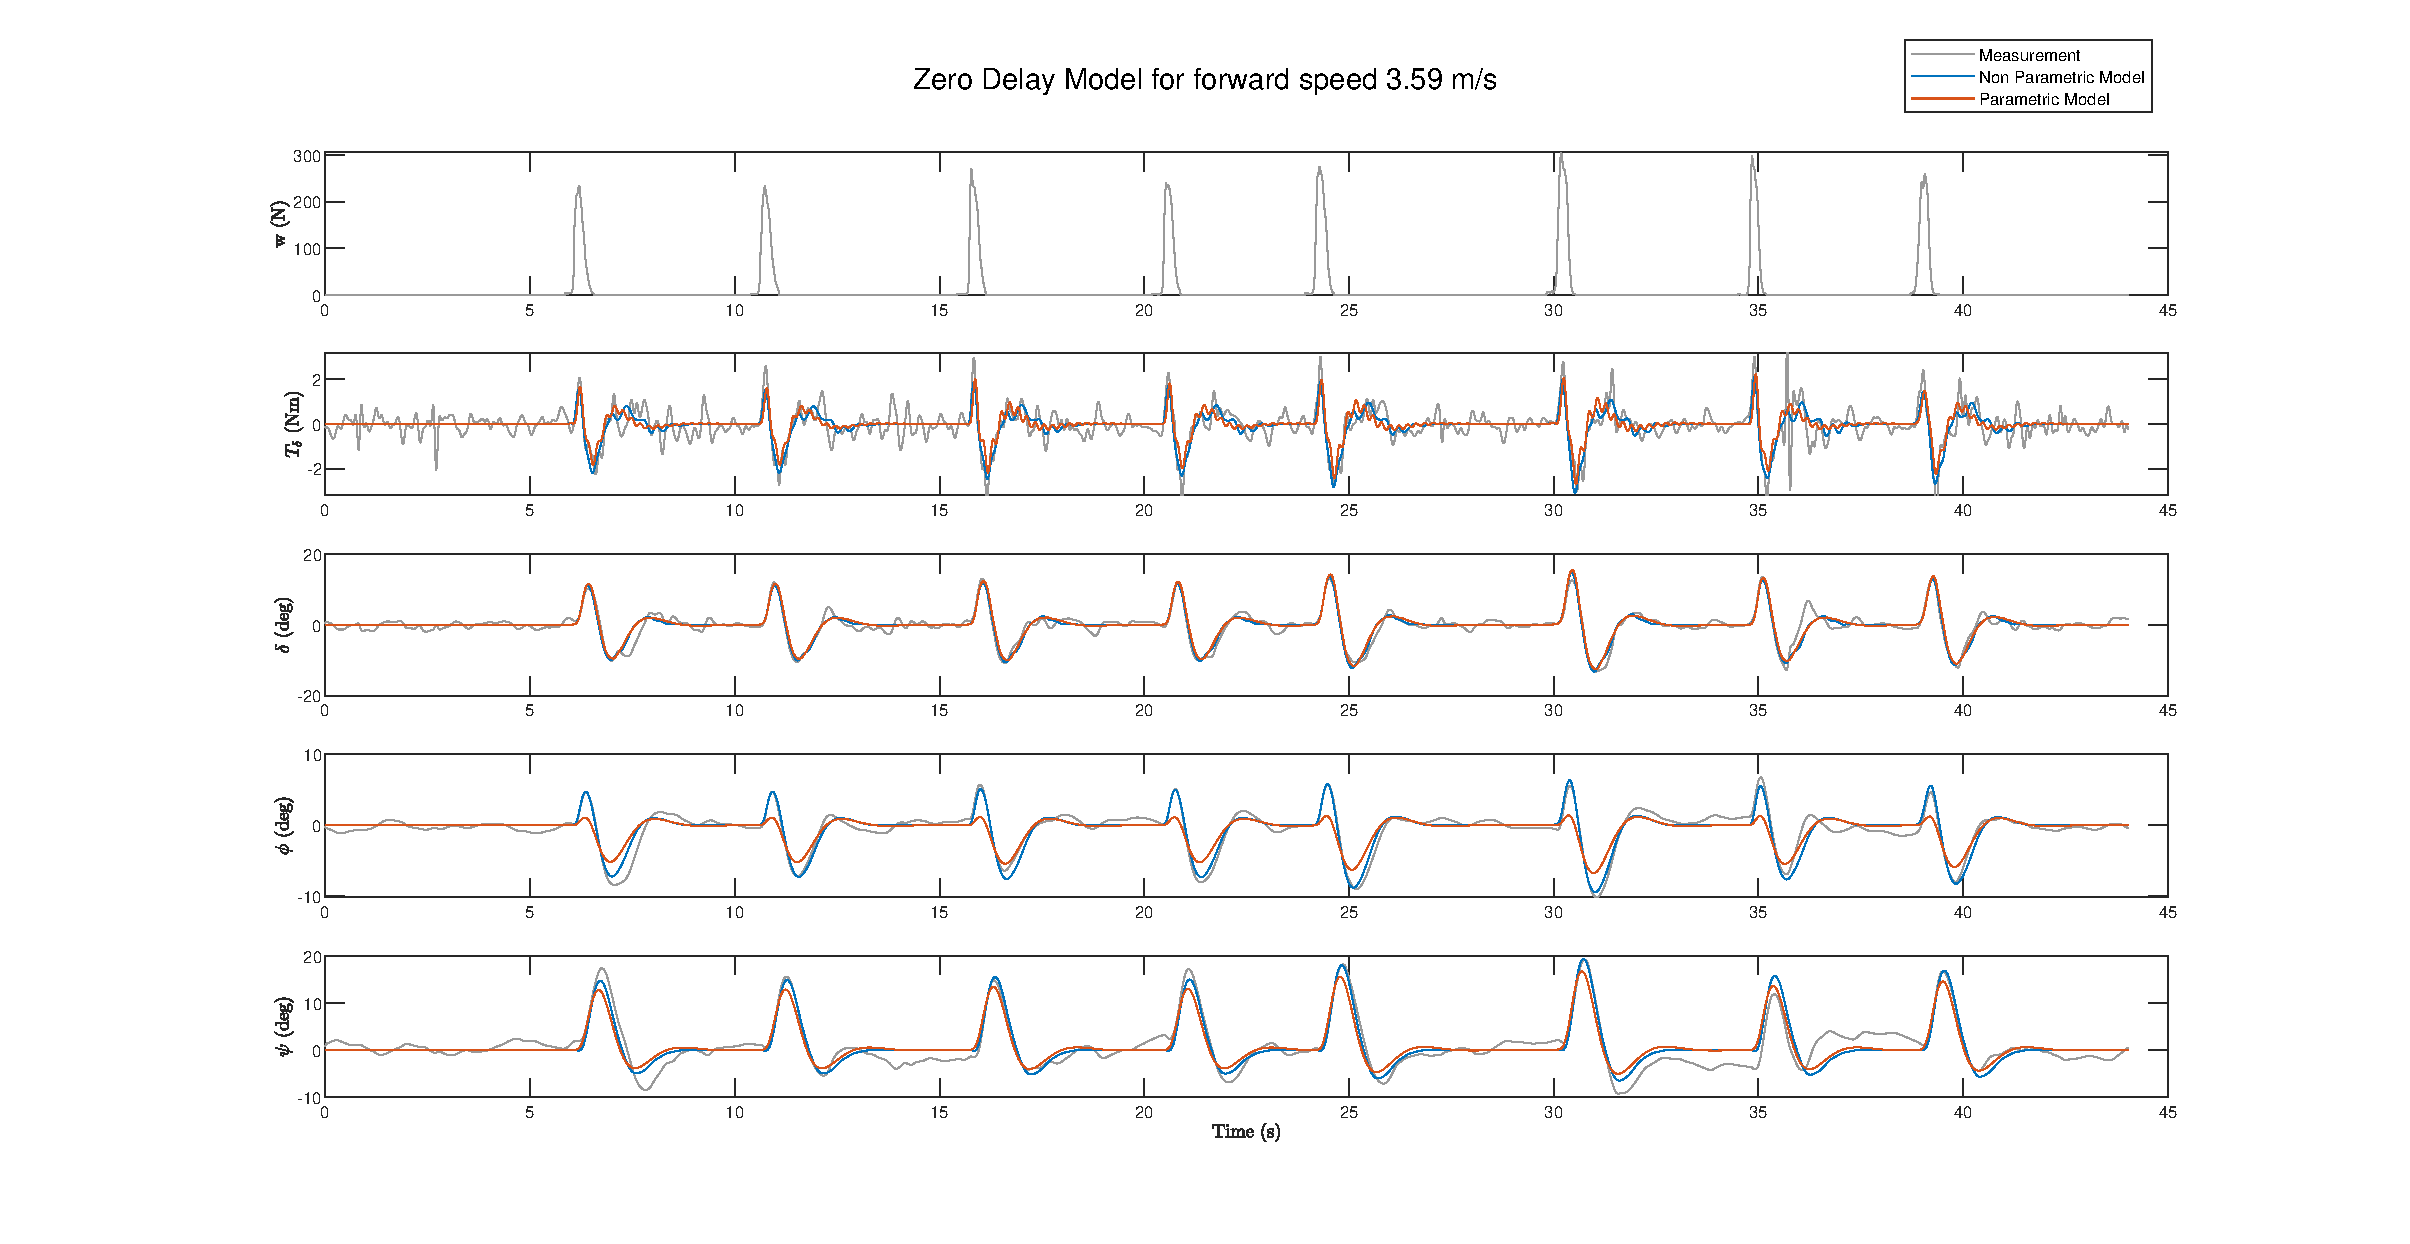
\includegraphics[width=\textwidth]{images/no_delay_result1.eps}
%     \caption{Comparison between parametric model output, non-parametric model ouput and measured signals for the speed level of 3.6 \si{\meter\per\second} for the case where torque feedback activated.}
%     \label{fig:paper5}
% \end{figure}

\begin{figure}[!h]
    \centering
    \begin{subfigure}[b]{\textwidth}
        \centering
        \makebox[\textwidth][c]{ 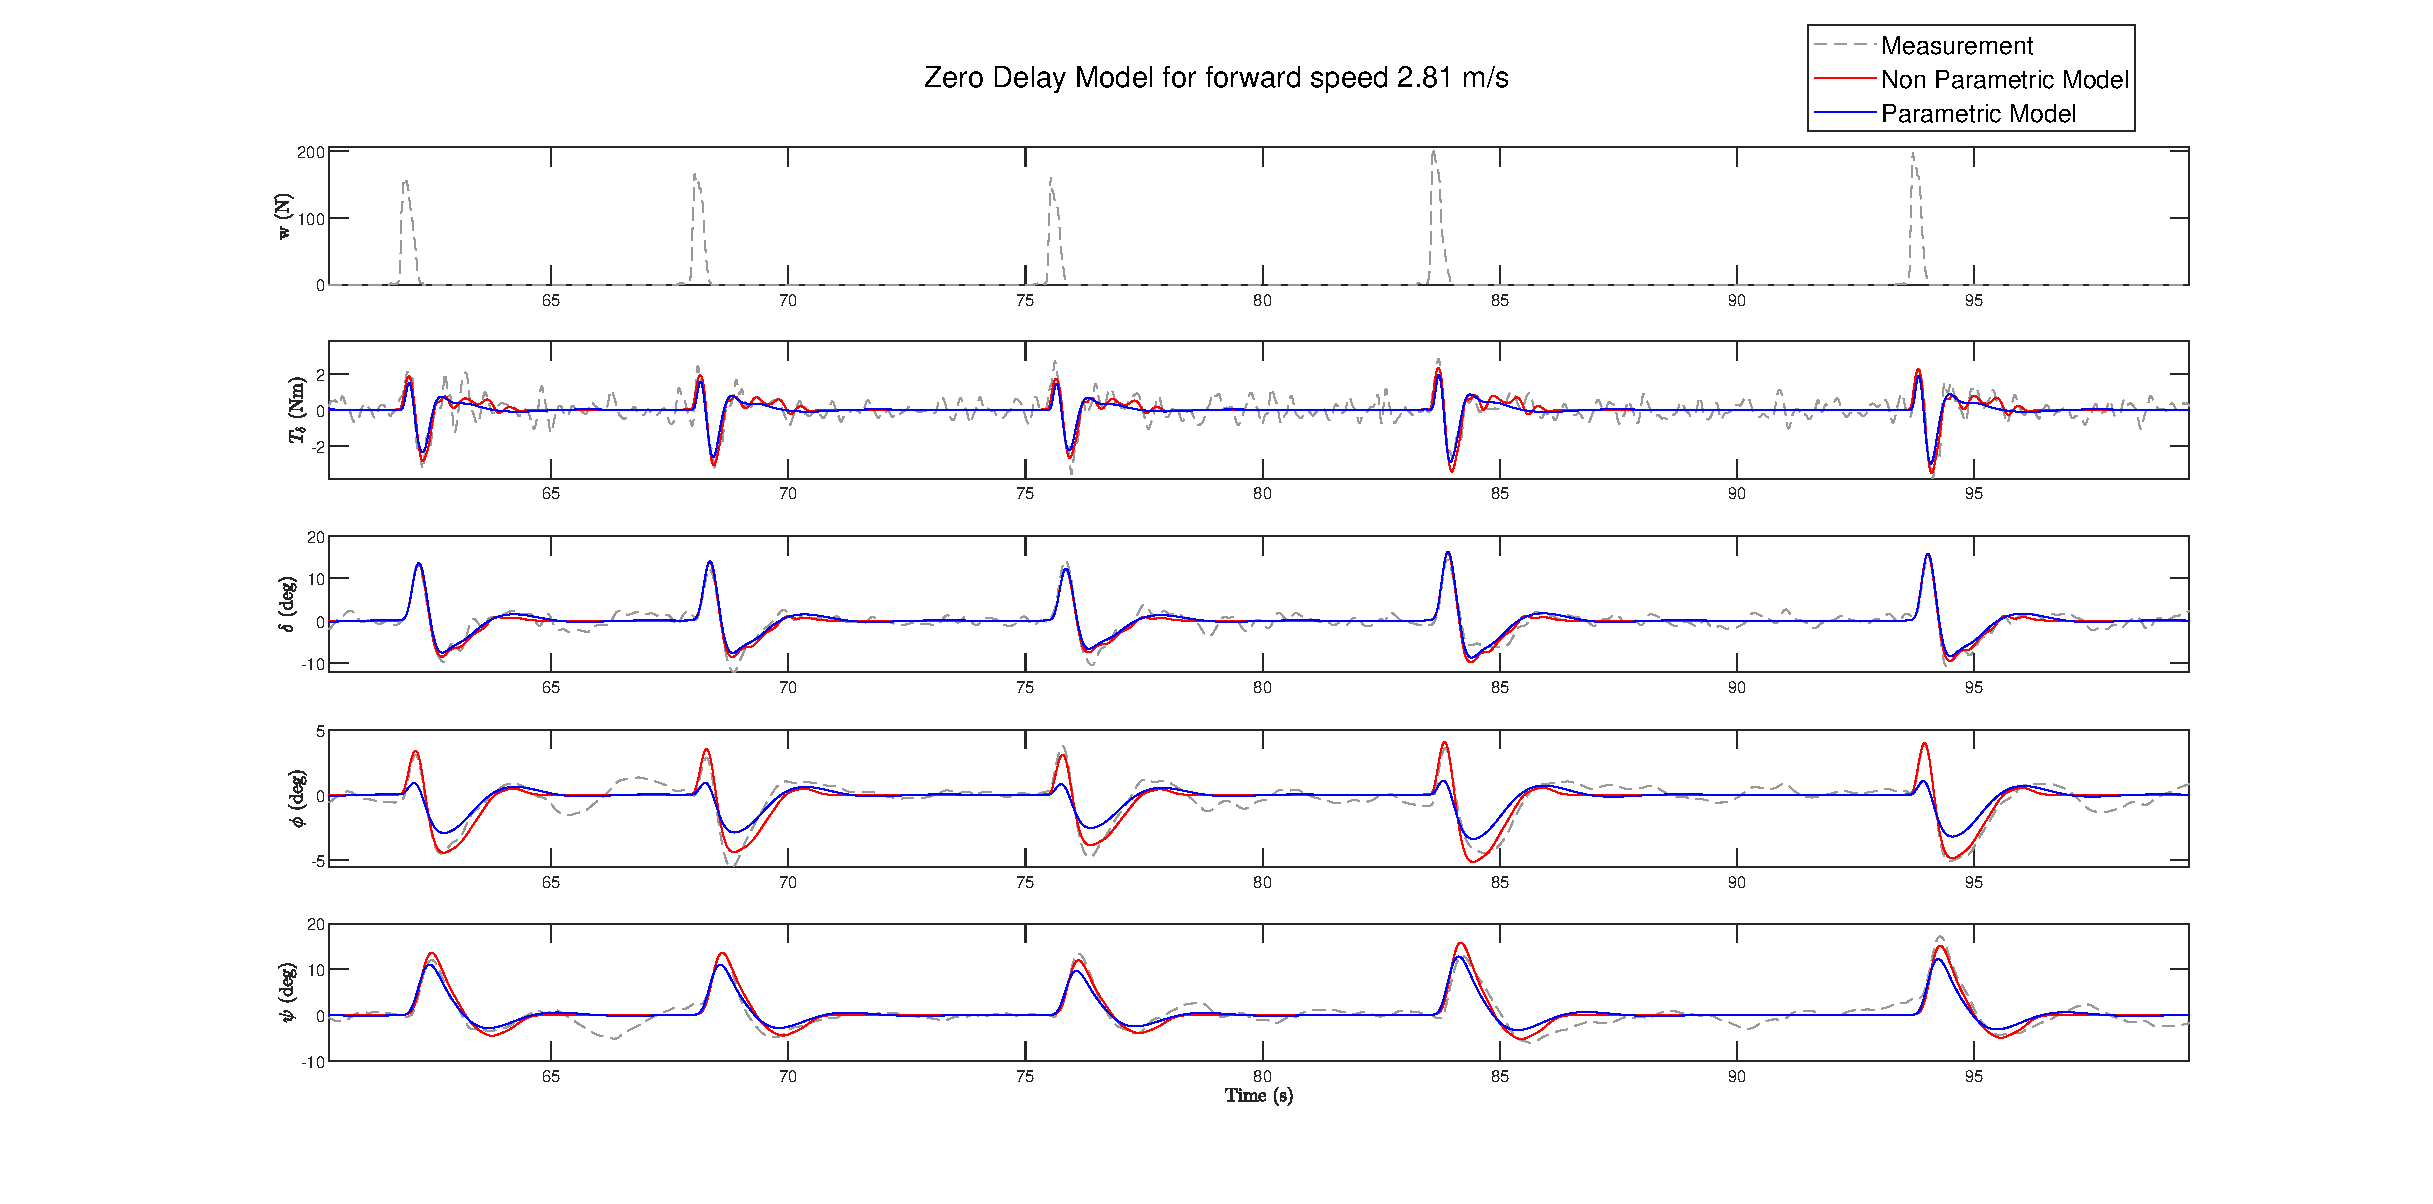
\includegraphics[width=1.4\textwidth]{images/raw_fit_plots/nodelay_28.eps}}
        \caption{}
        \label{fig:zdm_fit1}
    \end{subfigure}
    \begin{subfigure}[b]{\textwidth}
        \centering
        \makebox[\textwidth][c]{ 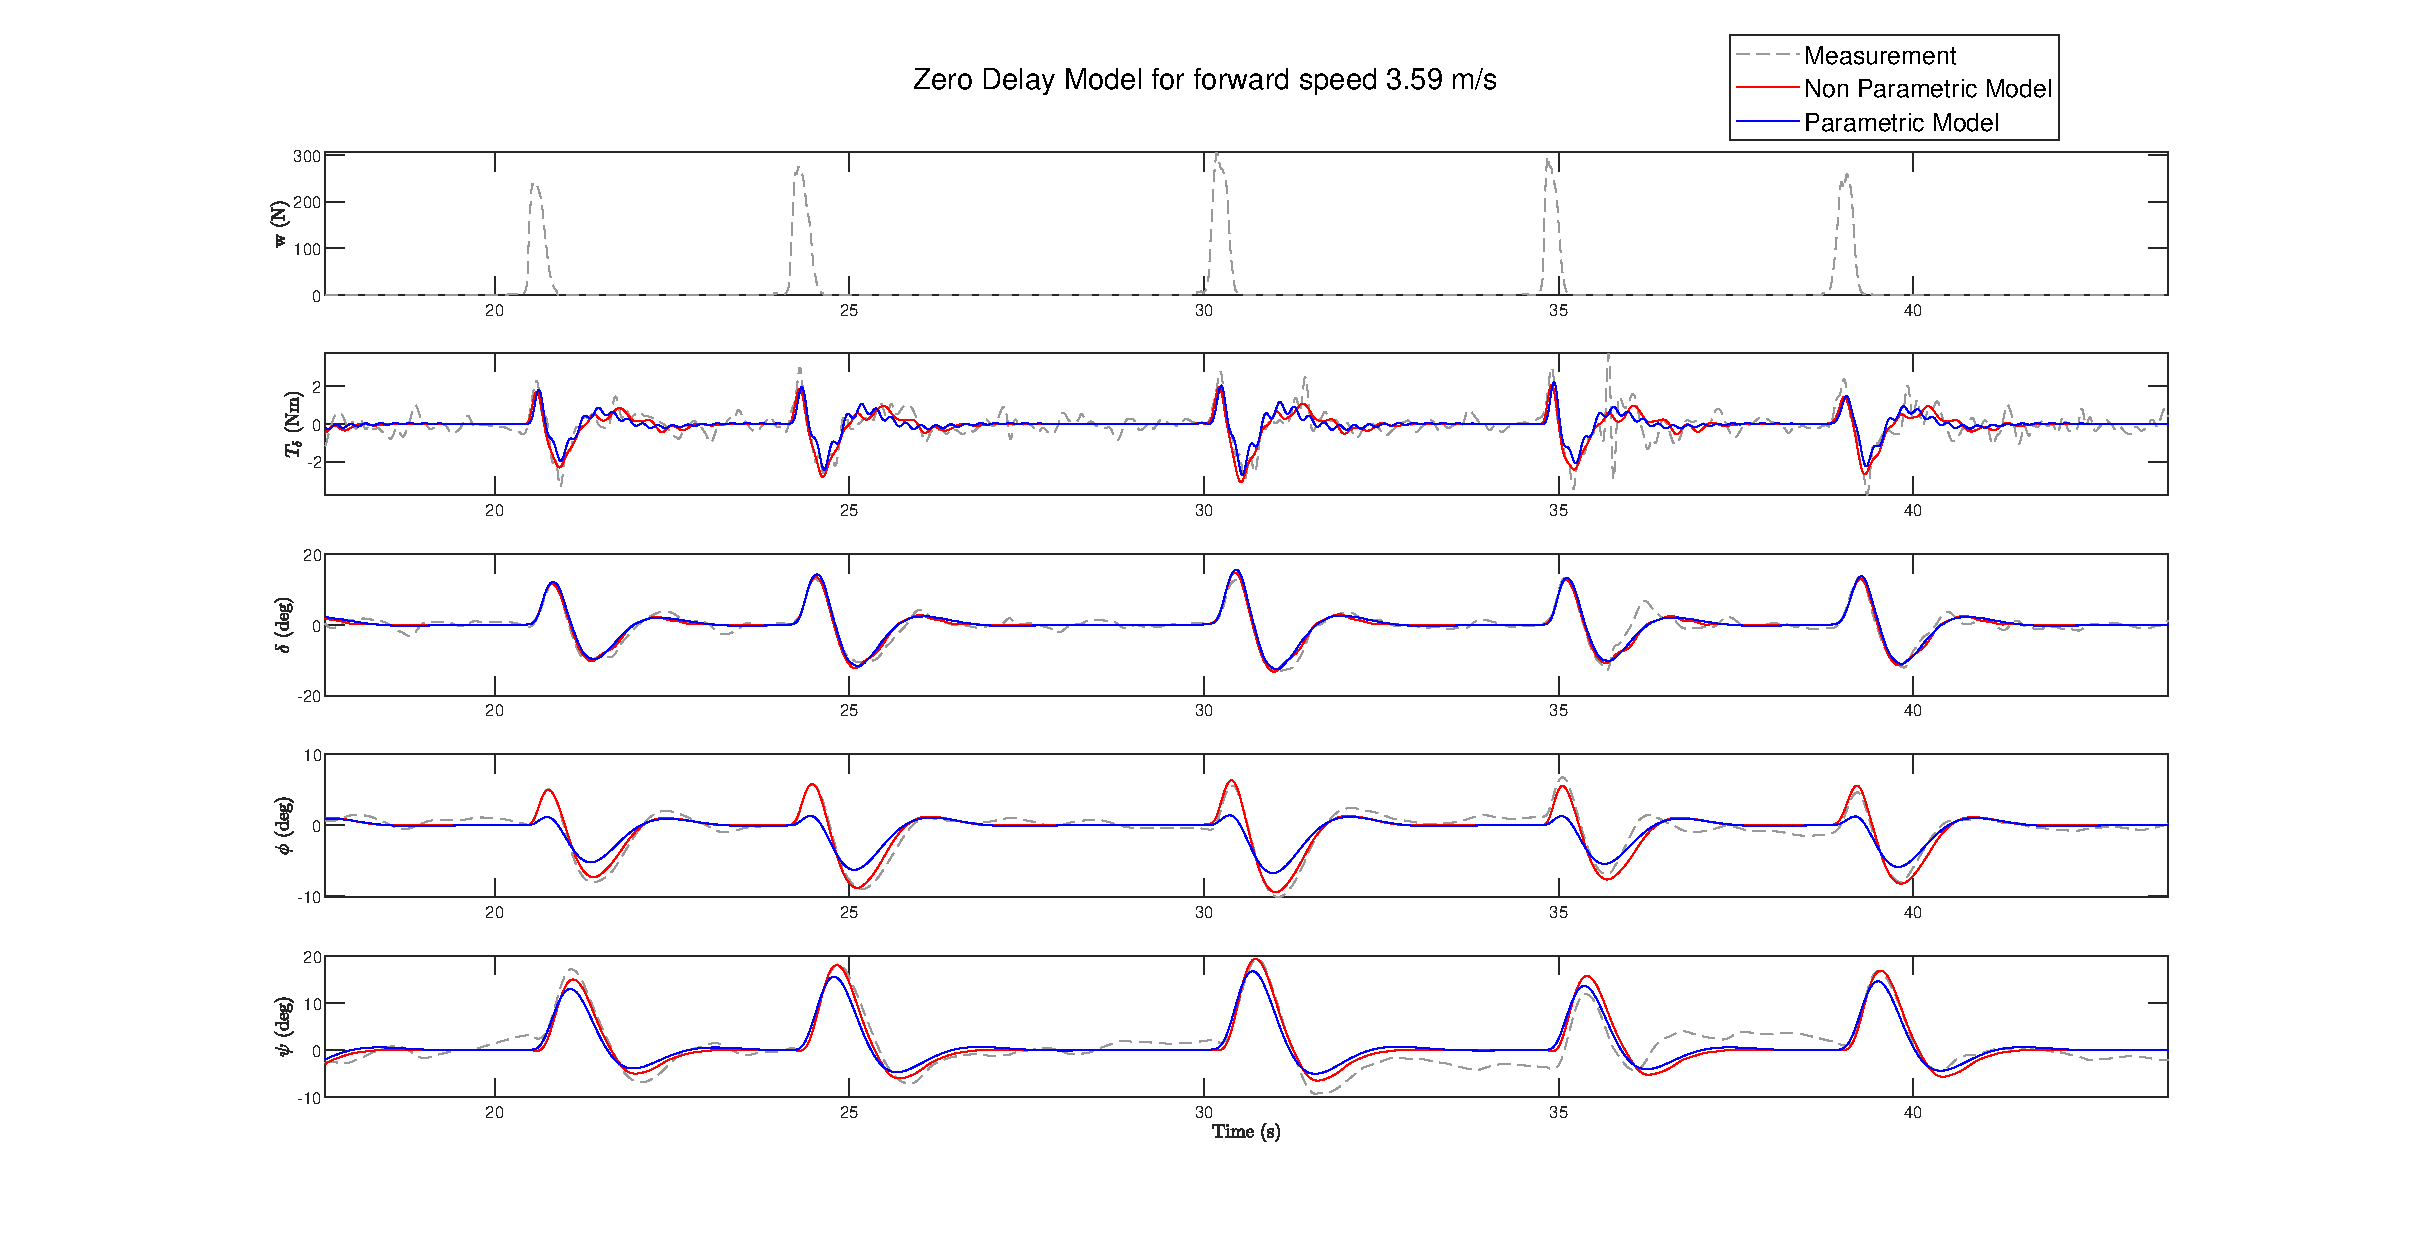
\includegraphics[width=1.4\textwidth]{images/raw_fit_plots/nodelay_36.eps}}
        \caption{}
        \label{fig:zdm_fit2}
    \end{subfigure}
    
    \caption{Comparison between parametric model output (Zero Delay Model), non-parametric model output and measured signals for the two lowest speed levels for the case where torque feedback is present in the rider control model and bicycle is operating under the "haptics on" dynamics.}
    \label{fig:zdm_fitA}
 \end{figure}

 \begin{figure}
    \centering
    \begin{subfigure}[b]{\textwidth}
        \centering
        \makebox[\textwidth][c]{ 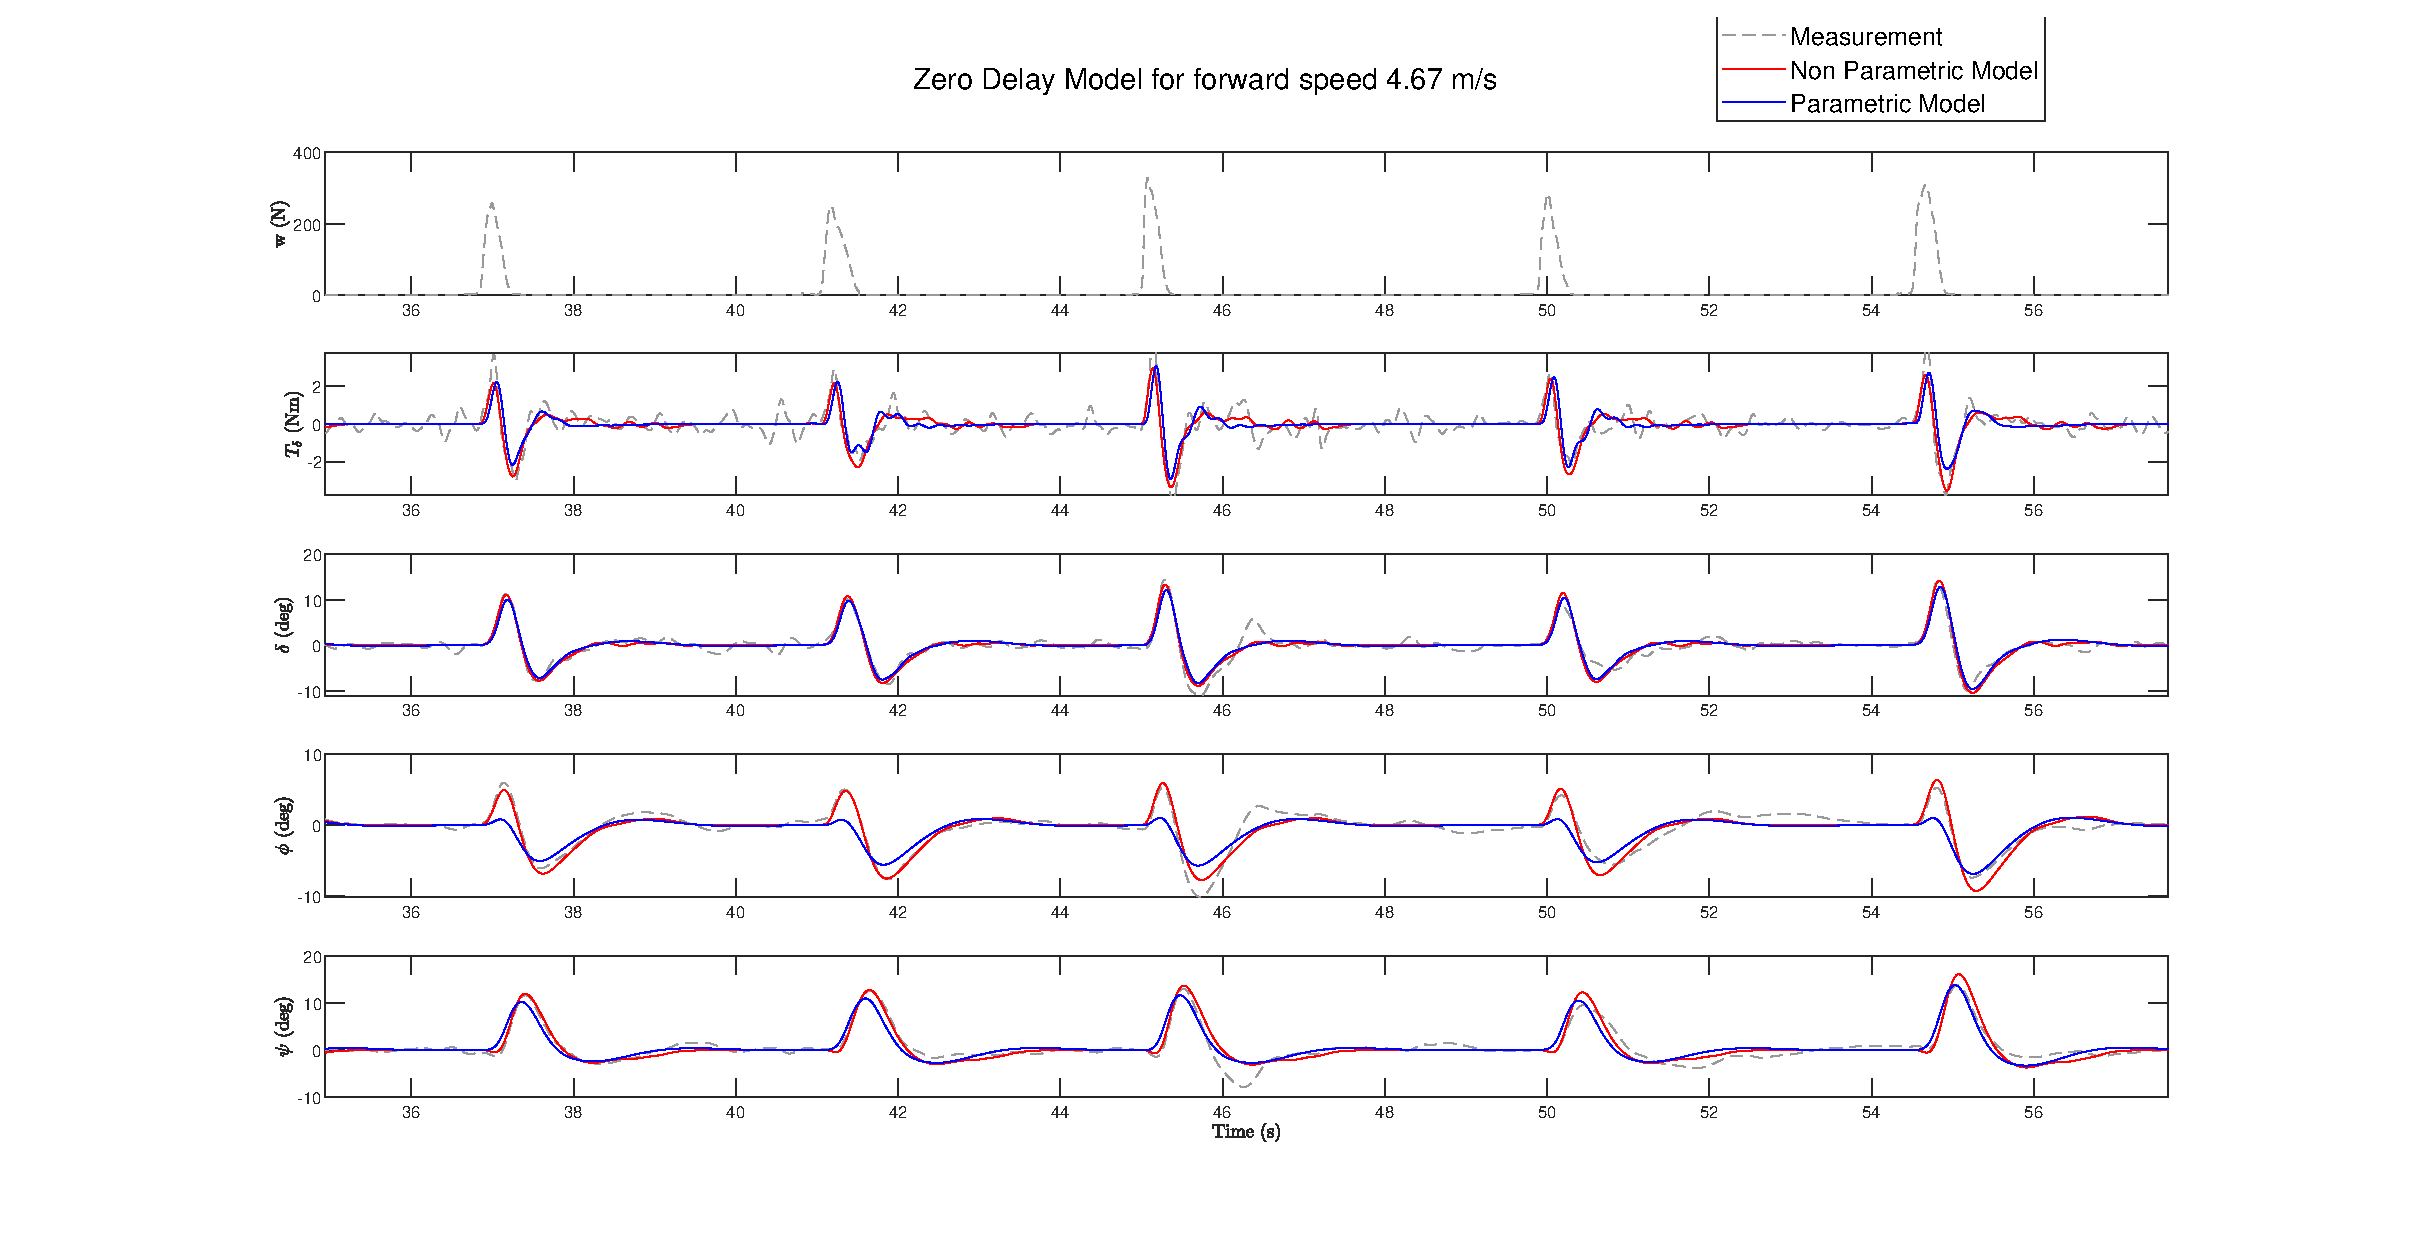
\includegraphics[width=1.4\textwidth]{images/raw_fit_plots/nodelay_46.eps}}
        \caption{}
        \label{fig:zdm_fit3}
    \end{subfigure}
    \begin{subfigure}[b]{\textwidth}
        \centering
        \makebox[\textwidth][c]{ 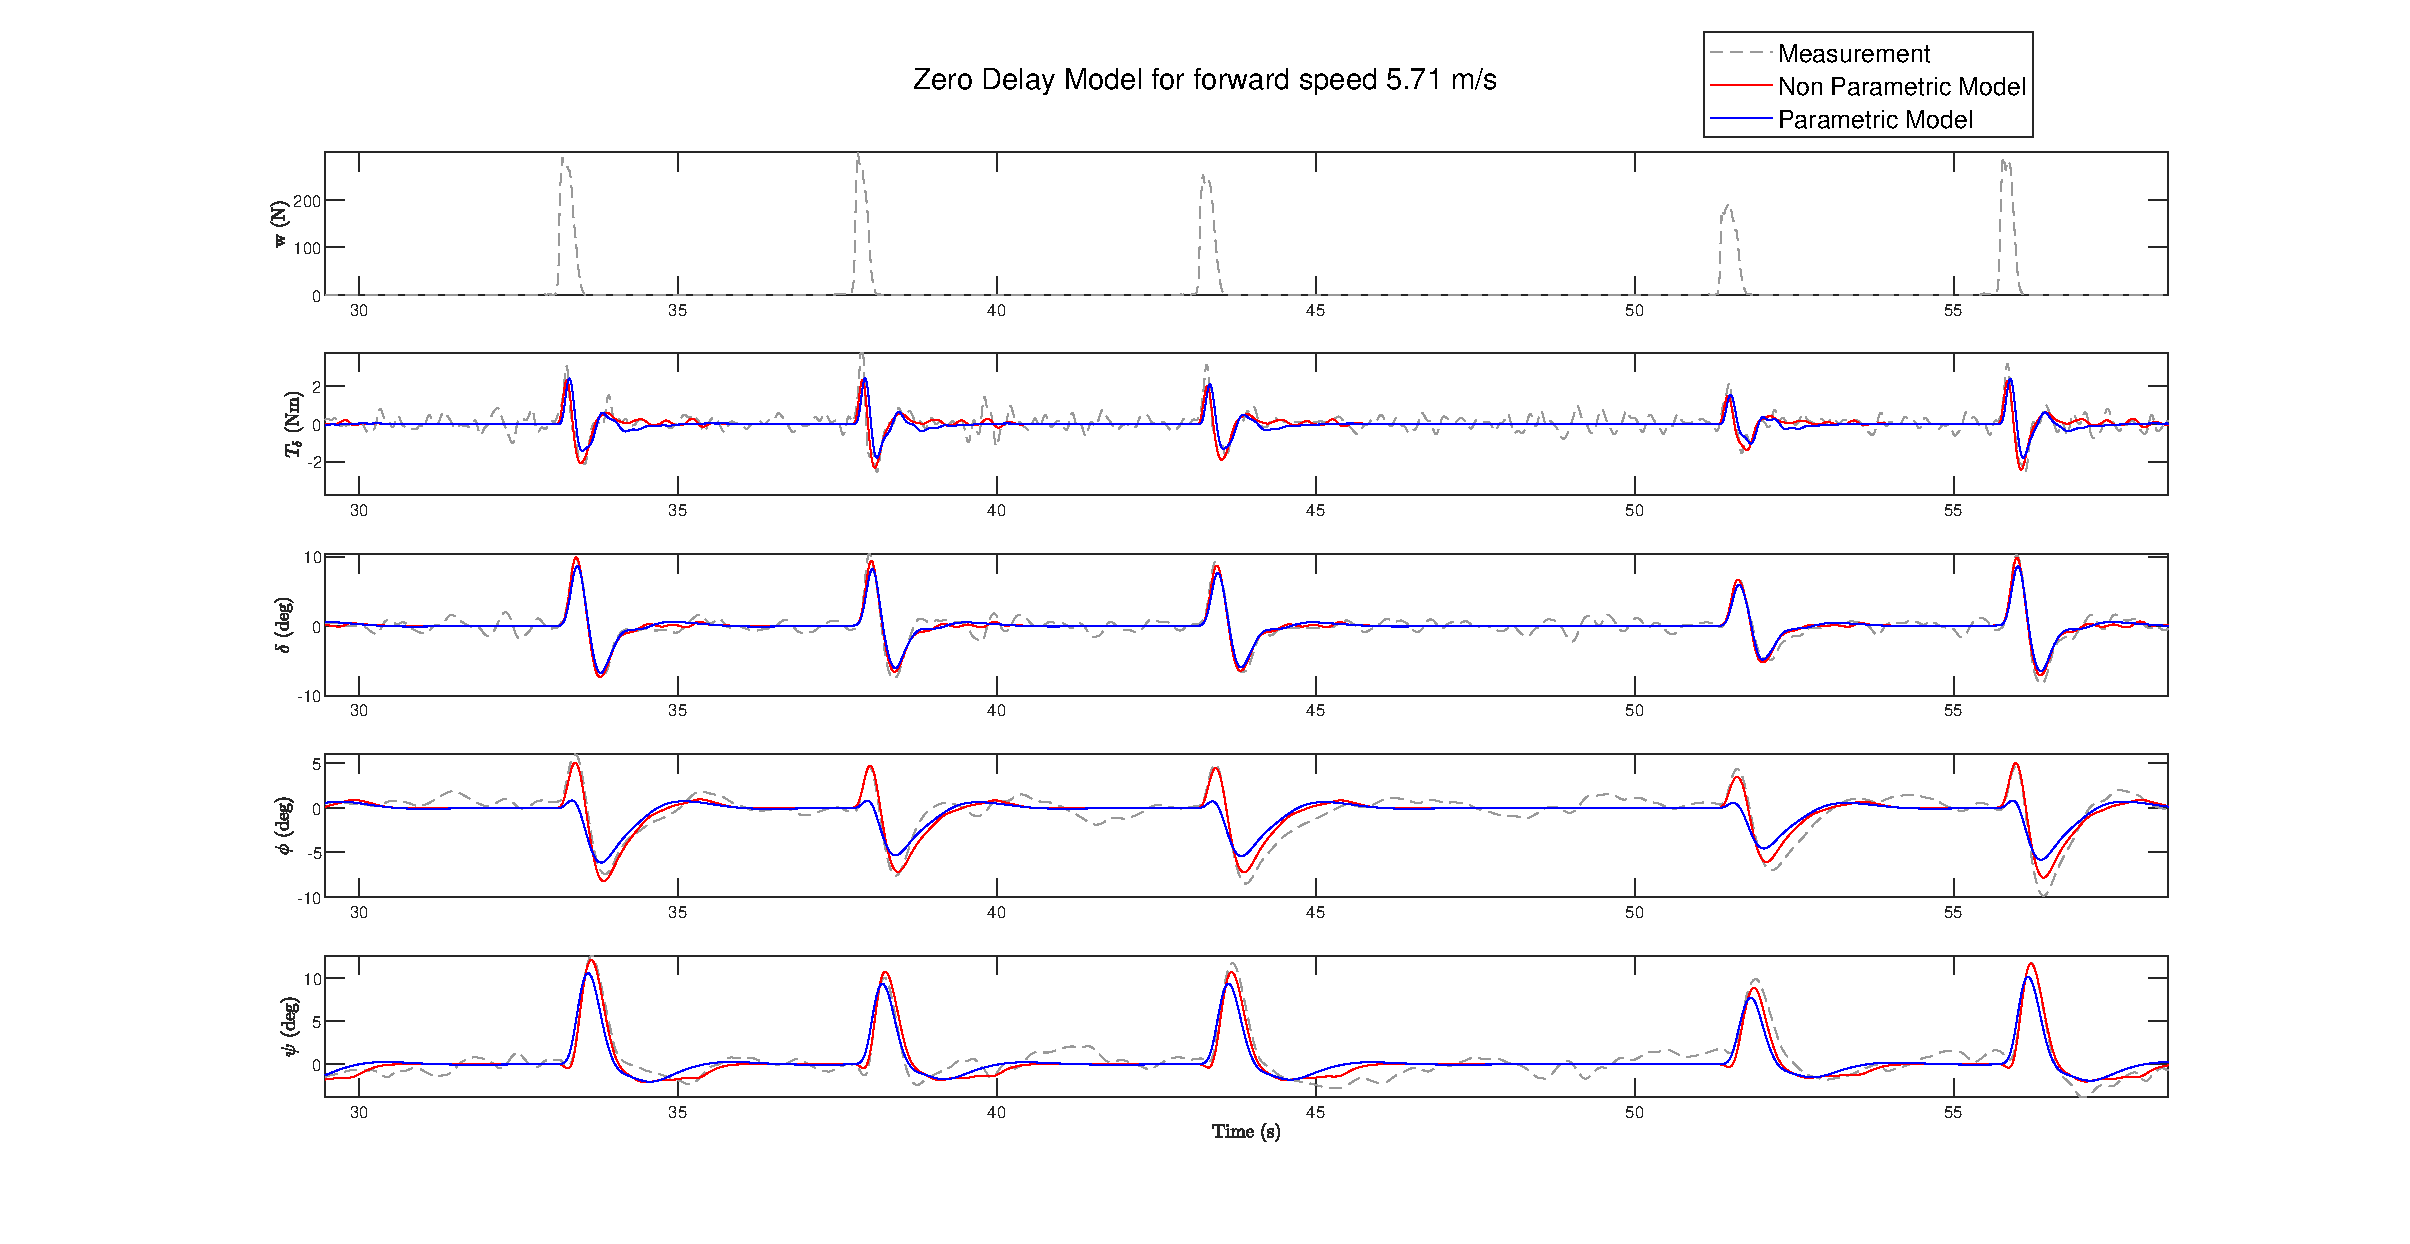
\includegraphics[width=1.4\textwidth]{images/raw_fit_plots/nodelay_57.eps}}
        \caption{}
        \label{fig:zdm_fit4}
    \end{subfigure}
    
    \caption{Comparison between parametric model output (Zero Delay Model), non-parametric model output and measured signals for the two highest speed levels for the case where torque feedback is present in the rider control model and bicycle is operating under the "haptics on" dynamics.}
    \label{fig:zdm_fitB}
 \end{figure}
From the coefficient of variation, no real difference between the levels of normalized uncertainty is noted. However, \ensuremath{\mathit{VAF}_\delta} drops more than 15-20\% when \ensuremath{T_\delta} feedback is turned off (see \cref{tb:no_delay}), which indicates significant impact on the fit. Additionally,  the steering angle and torque response   becomes significantly more oscillatory when \ensuremath{{T_\delta}} feedback is turned off (see \cref{fig:paper6}). Roll stabilization performance does not seem to be affected, however steering effort considerably does. Regarding the haptics off case, where the intent is to simulate the steering feel the participants experienced in the second experimental condition, the level of steering fit degradation is small (\ensuremath{<3\%}).

\begin{figure}[!h]
    \centering
    \captionsetup{justification=centering,margin=2cm}

    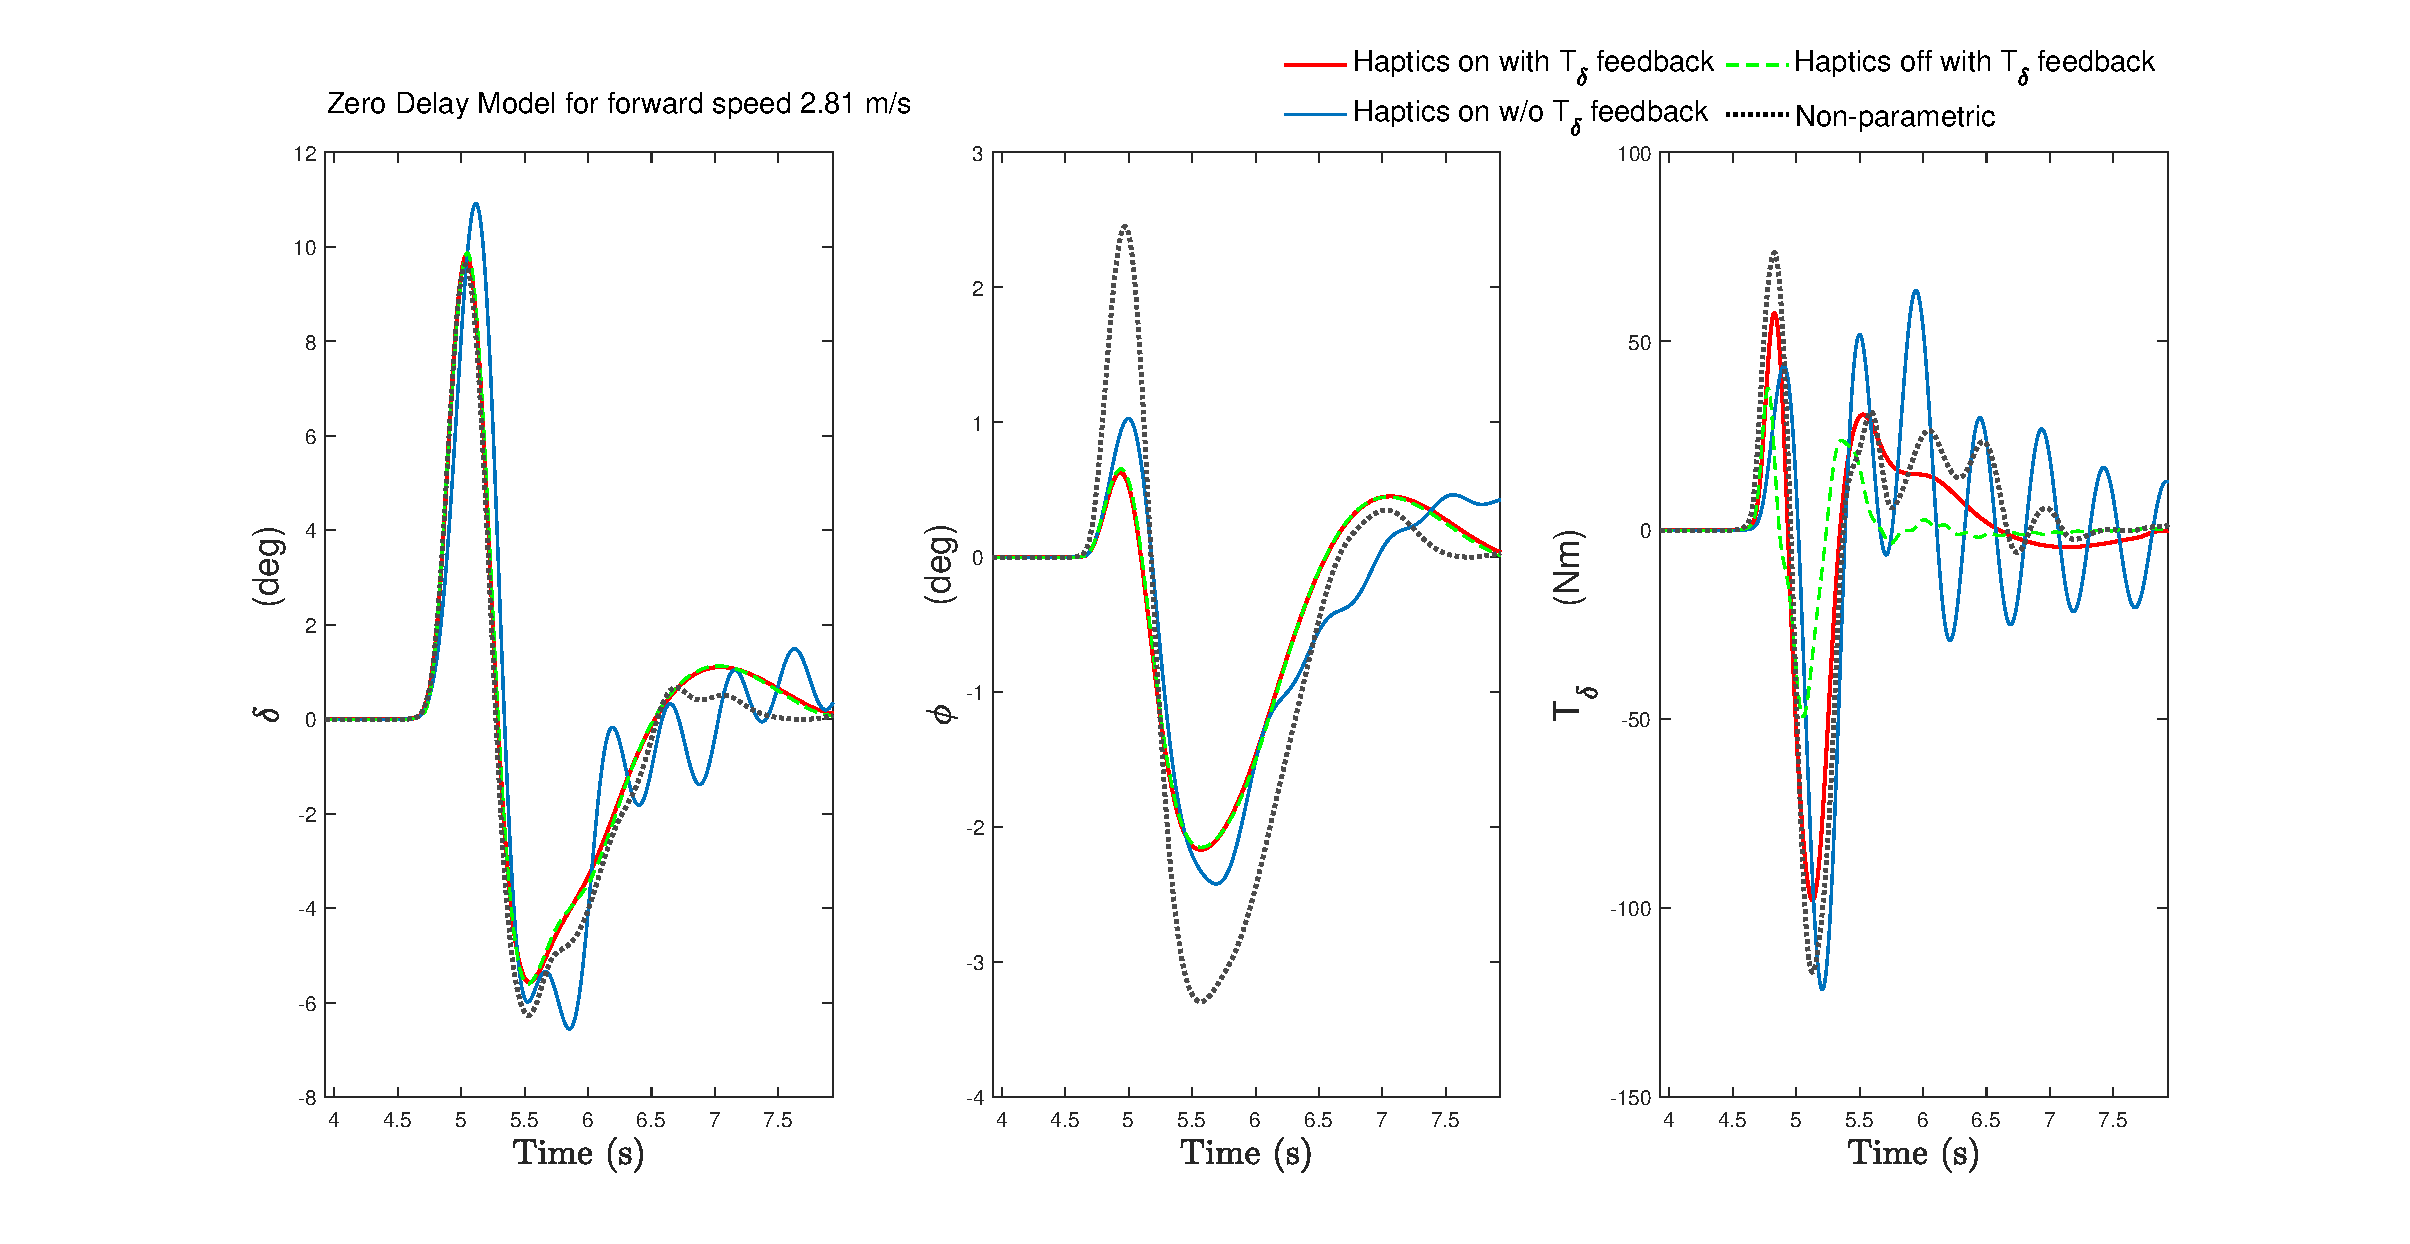
\includegraphics[width=\textwidth]{images/fb_compare_plots/no_delay_fb_compare28.eps}
    \caption{Steering, roll angles and input rider torque compared among torque feedback levels  for the forward speed of 2.81 \si{\meter\per\second} in the Zero Delay Model. Response of the first disturbance in the run is shown.}
    \label{fig:paper6}
\end{figure}



\subsection{Variable Delay Model}
The same procedure is repeated for the gray box model but now introducing  delays in all feedback pathways. For \ensuremath{\delta} and \ensuremath{\dot{\delta}} which are attributed to the muscle spindle sensors and for the torque feedback which is attributed to the golgi tendon organs  a delay of 25 \si{\milli\second} is chosen \cite{van2002identification,de2002adaptation}. For the feedback states attributed to visual feedback such as the roll angle \ensuremath{\phi} and yaw angle \ensuremath{\psi} a much greater delay of 200 \si{\milli\second} is chosen \cite{kawakami2002visual}. Finally for  the vestibular roll rate feedback a delay of 50 \si{\milli\second} is implemented \cite{barnett2013vestibular}. 

The results of the variable delay model for the median rider are presented in \cref{tb:variable}.  Despite the fact that significant delay is introduced into the system the torque feedback loop manages to compensate maintaining a \ensuremath{\mathit{VAF}_\delta} of over 90 \% for low speed levels (see \cref{tb:variable} and \cref{fig:dm_fitA}). In \cref{fig:dm_fitA,fig:dm_fitB} the delayed response of the simulated compared to the real rider is visible between the red and blue lines in the rider torque graph. This is further exaggerated in the two remaining conditions resulting in much more oscillatory steering responses with a visible impact on roll stabilization (see \cref{fig:paper8}). The coefficient of variation of the \ensuremath{K_\delta} parameter in the haptics on with \ensuremath{T_\delta} feedback connected is the highest especially for the two highest speed levels, which indicates that this parameter is not significant for the fit. Between \ensuremath{{T_\delta}} feedback on and feedback off, a much larger drop in VAF is noted. Additionally, contrary to the zero delay model an equally significant drop in the fit is noted for the haptics off case. 






\begin{figure}[!h]
    \centering
    \begin{subfigure}[b]{\textwidth}
        \centering
        \makebox[\textwidth][c]{ 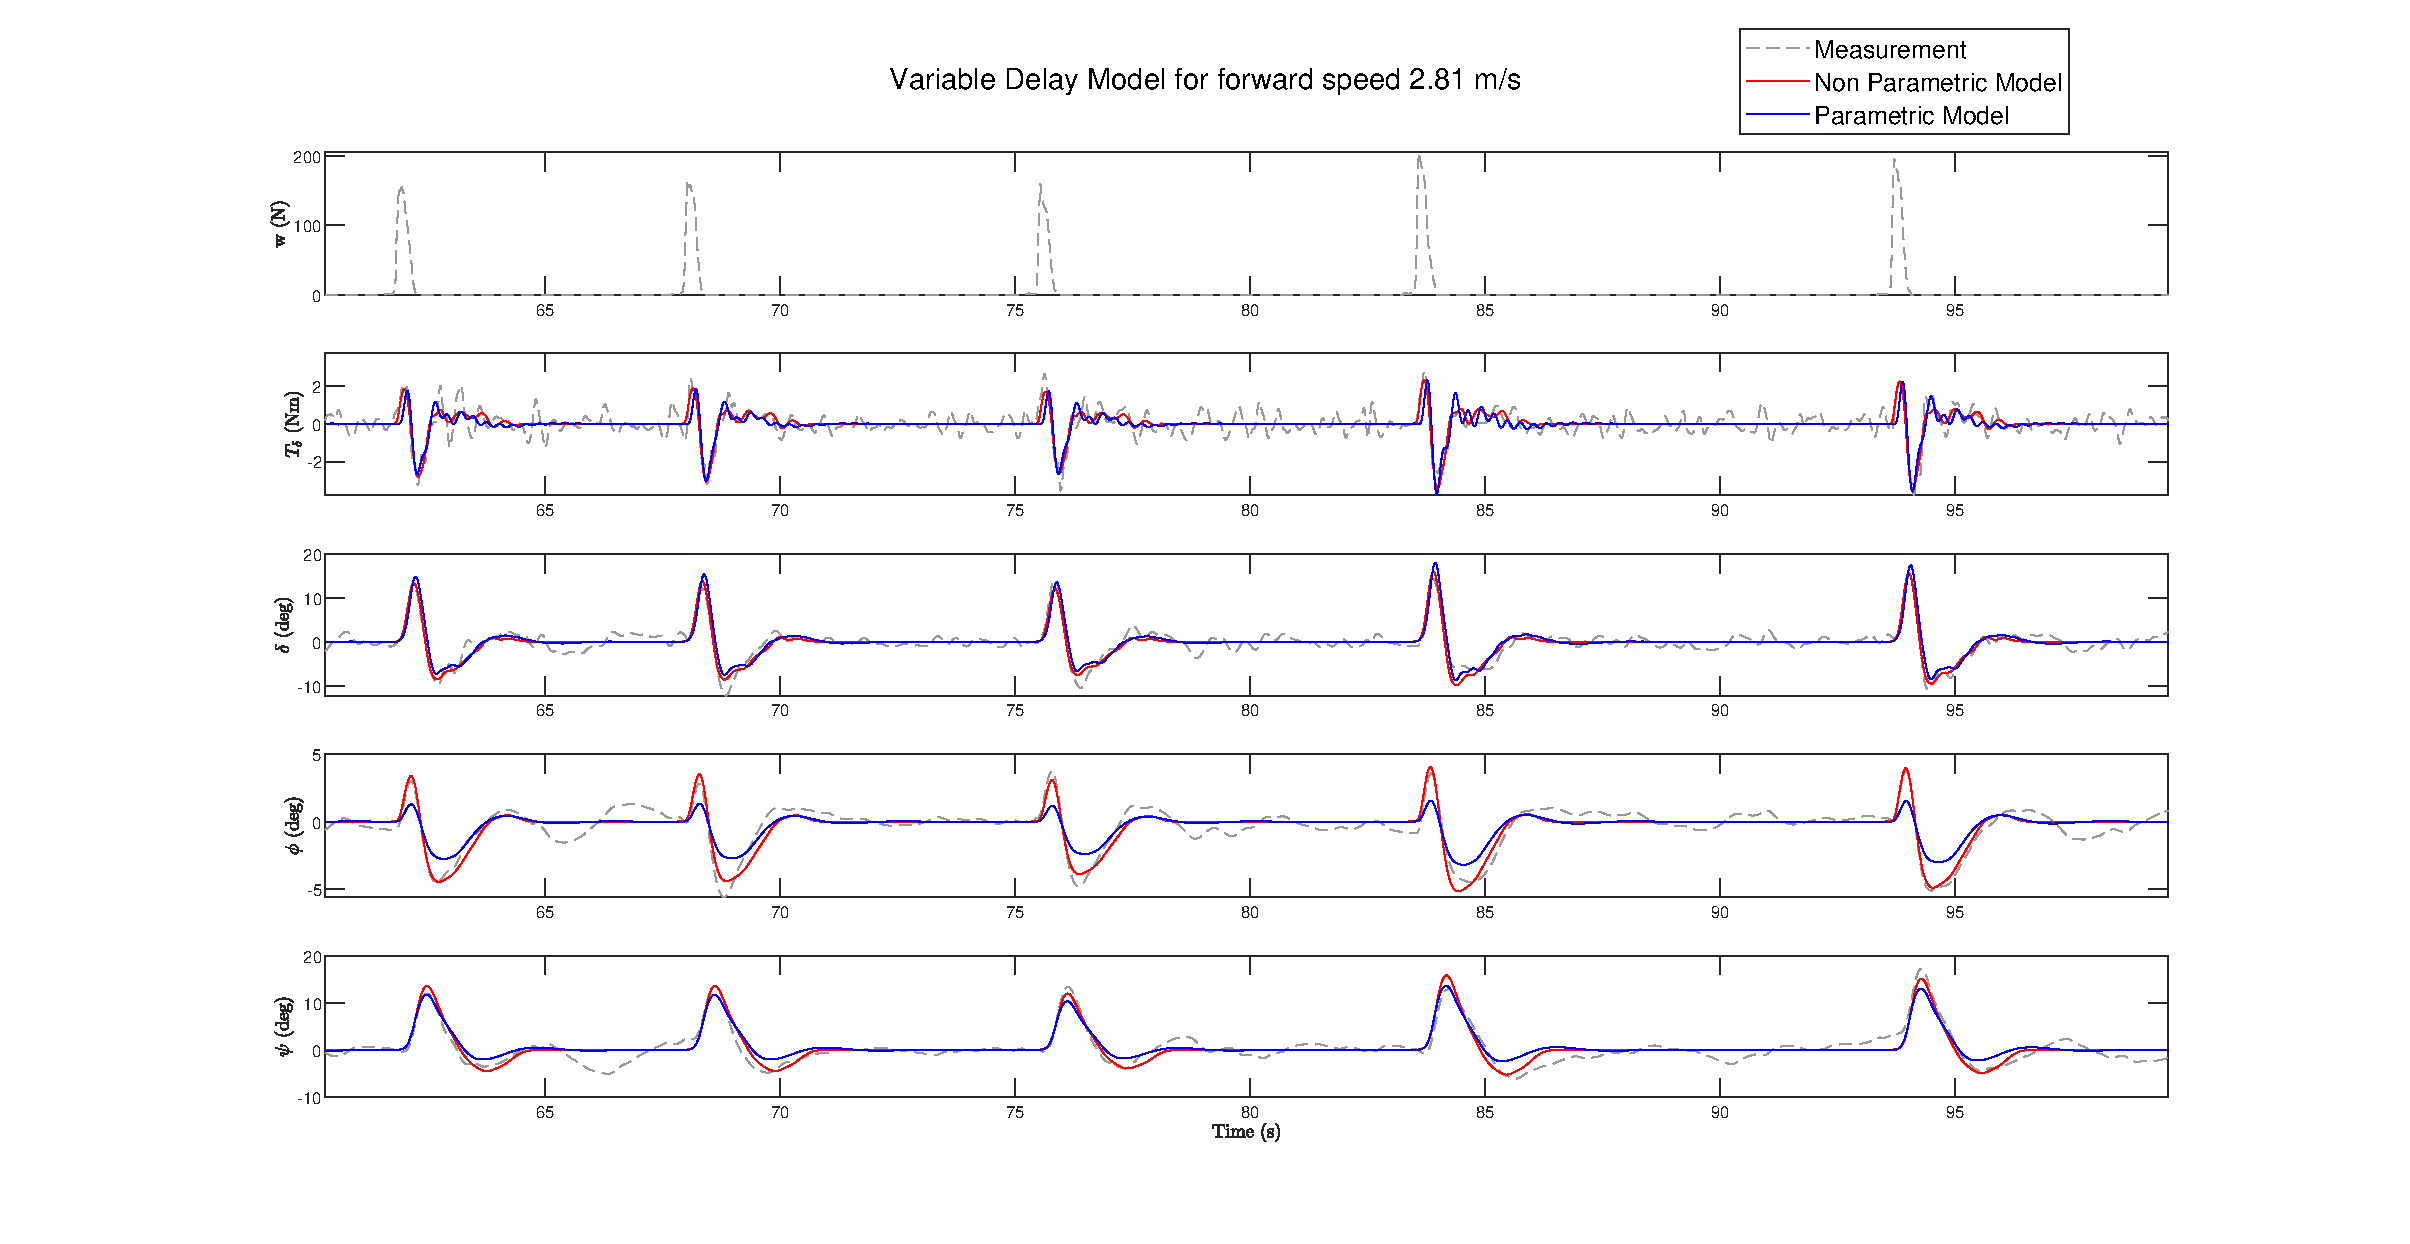
\includegraphics[width=1.4\textwidth]{images/raw_fit_plots/delay_28.eps}}
        \caption{}
        \label{fig:dm_fit1}
    \end{subfigure}
    \begin{subfigure}[b]{\textwidth}
        \centering
        \makebox[\textwidth][c]{ 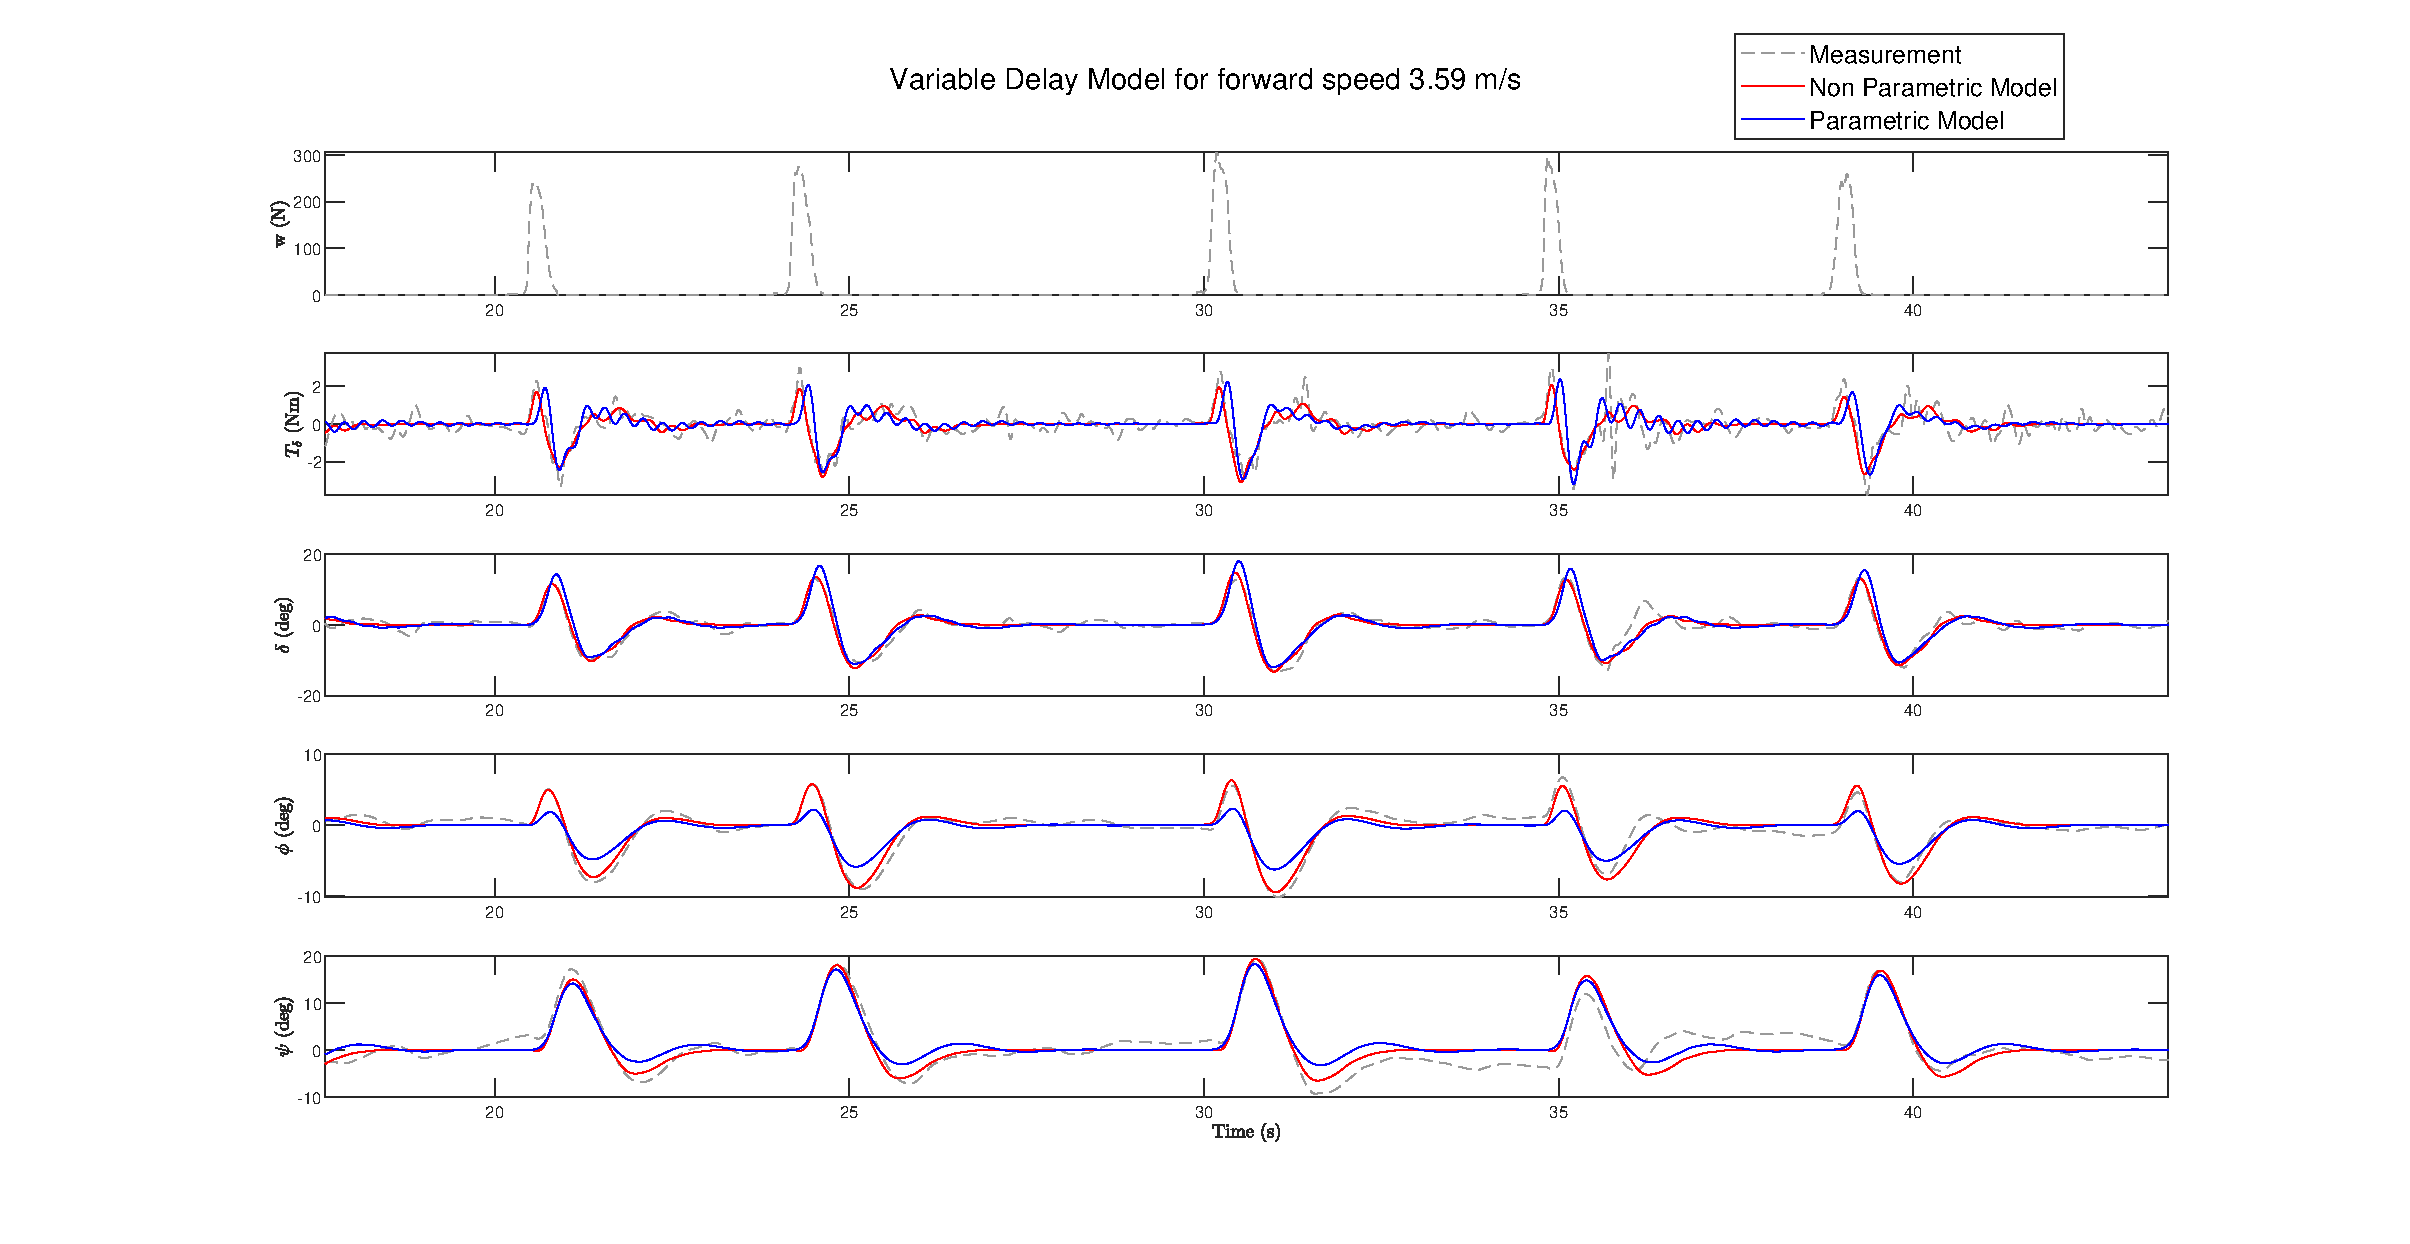
\includegraphics[width=1.4\textwidth]{images/raw_fit_plots/delay_36.eps}}
        \caption{}
        \label{fig:dm_fit2}
    \end{subfigure}
    
    \caption{Comparison between parametric model output (Variable Delay Model), non-parametric model output and measured signals for the two lowest speed levels for the case where torque feedback is present in the rider control model and bicycle is operating under the "haptics on" dynamics.}
    \label{fig:dm_fitA}
 \end{figure}

 \begin{figure}
    \centering
    \begin{subfigure}[b]{\textwidth}
        \centering
        \makebox[\textwidth][c]{ 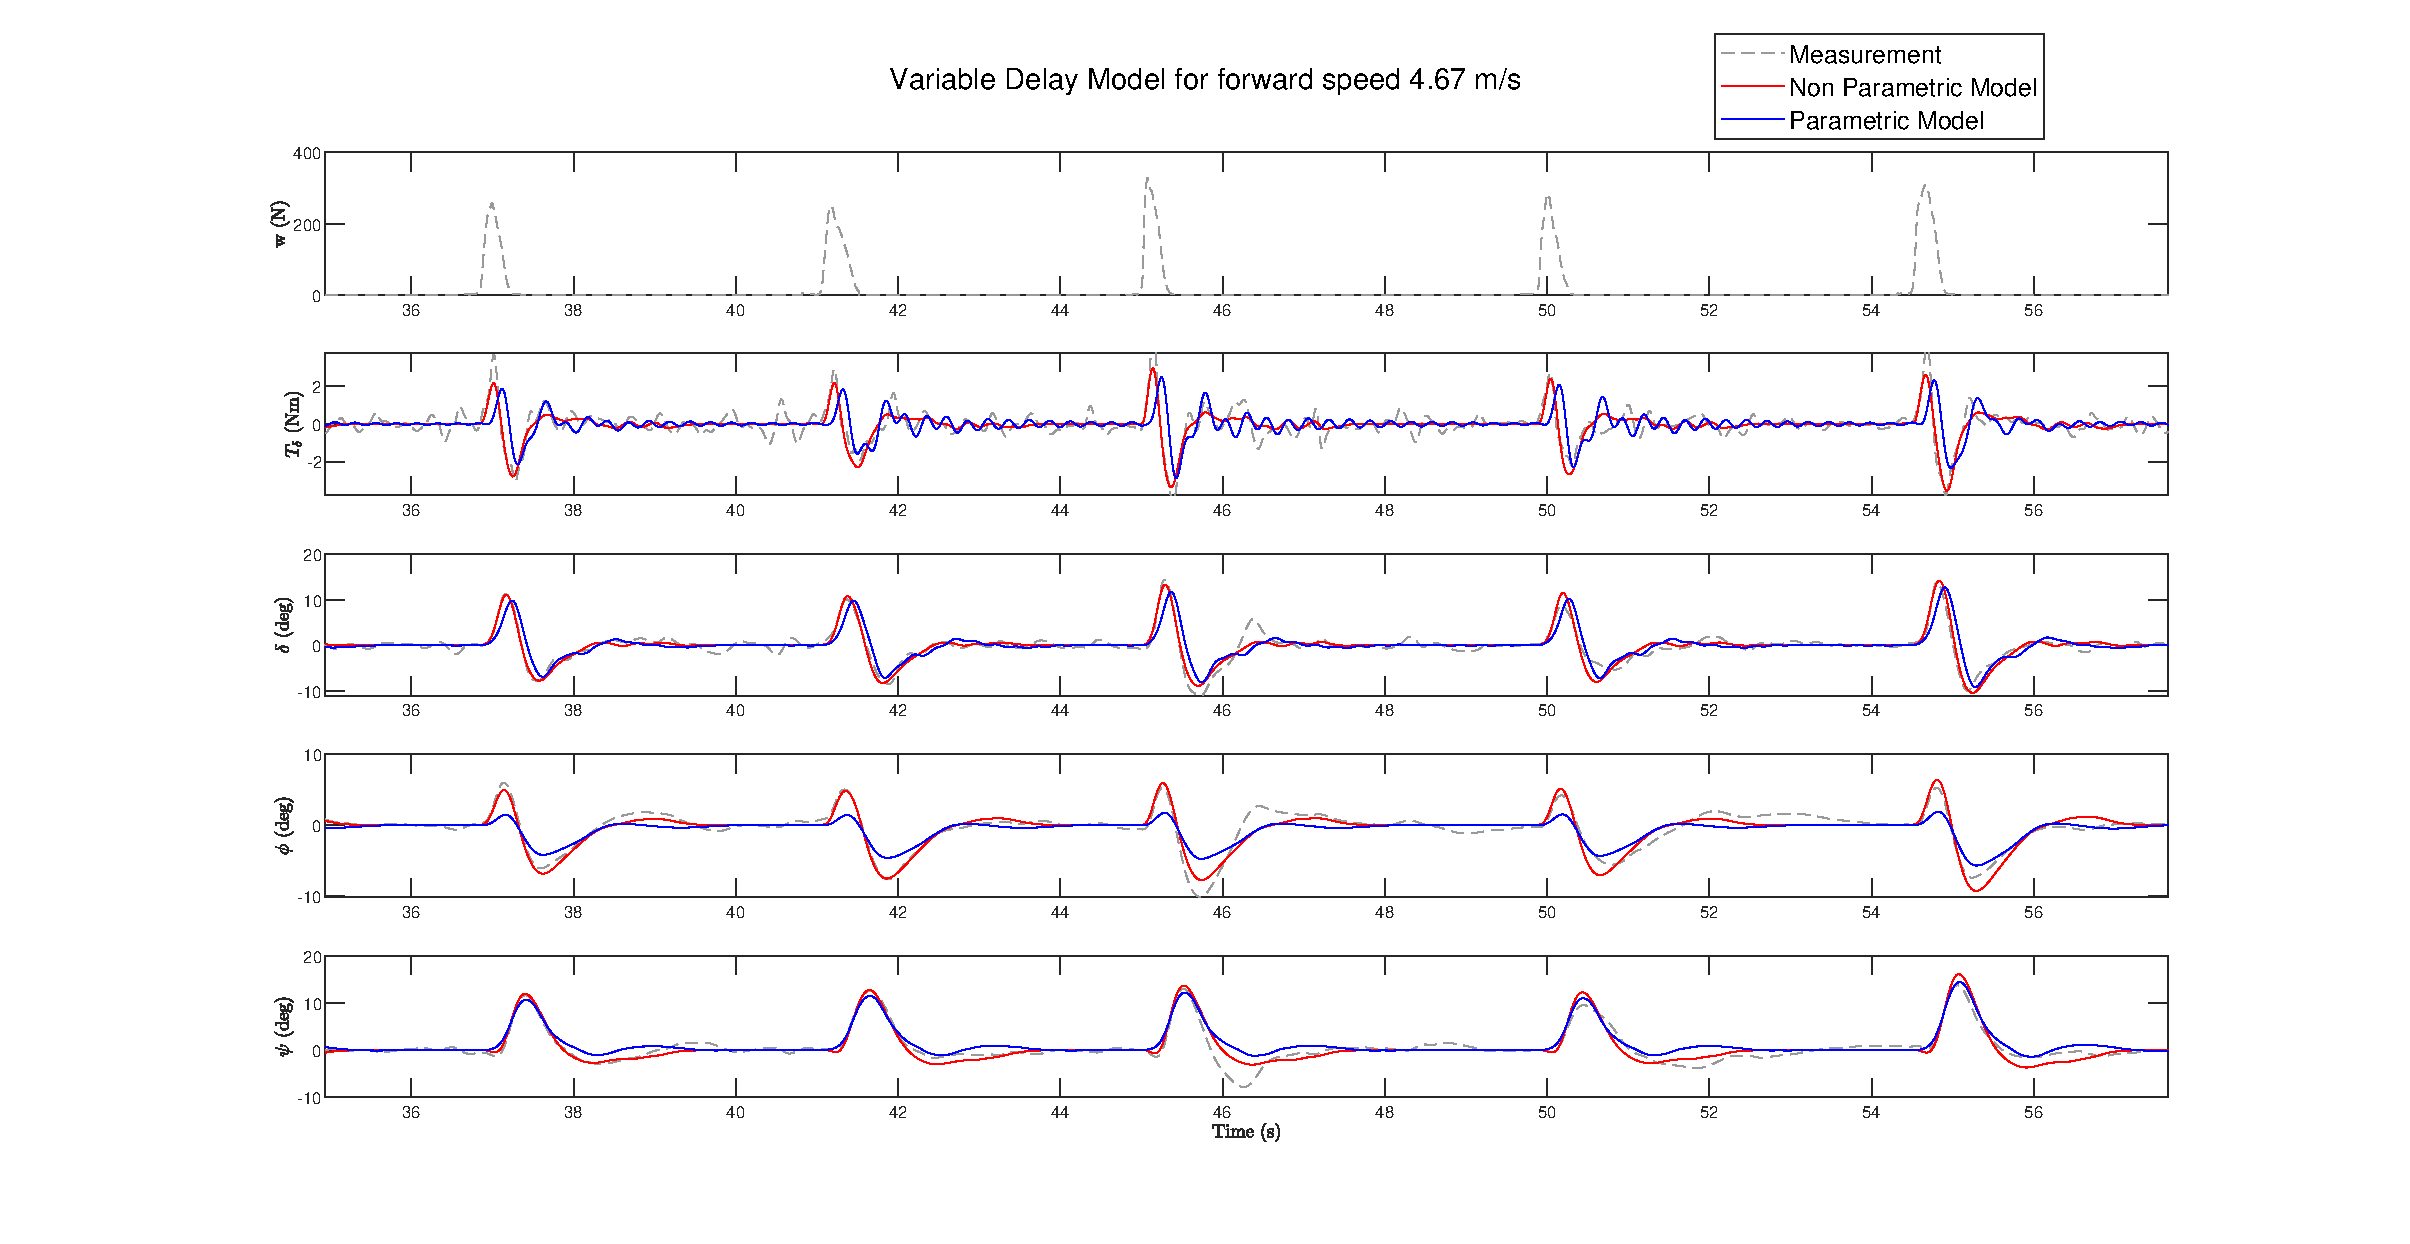
\includegraphics[width=1.4\textwidth]{images/raw_fit_plots/delay_46.eps}}
        \caption{}
        \label{fig:dm_fit3}
    \end{subfigure}
    \begin{subfigure}[b]{\textwidth}
        \centering
        \makebox[\textwidth][c]{ 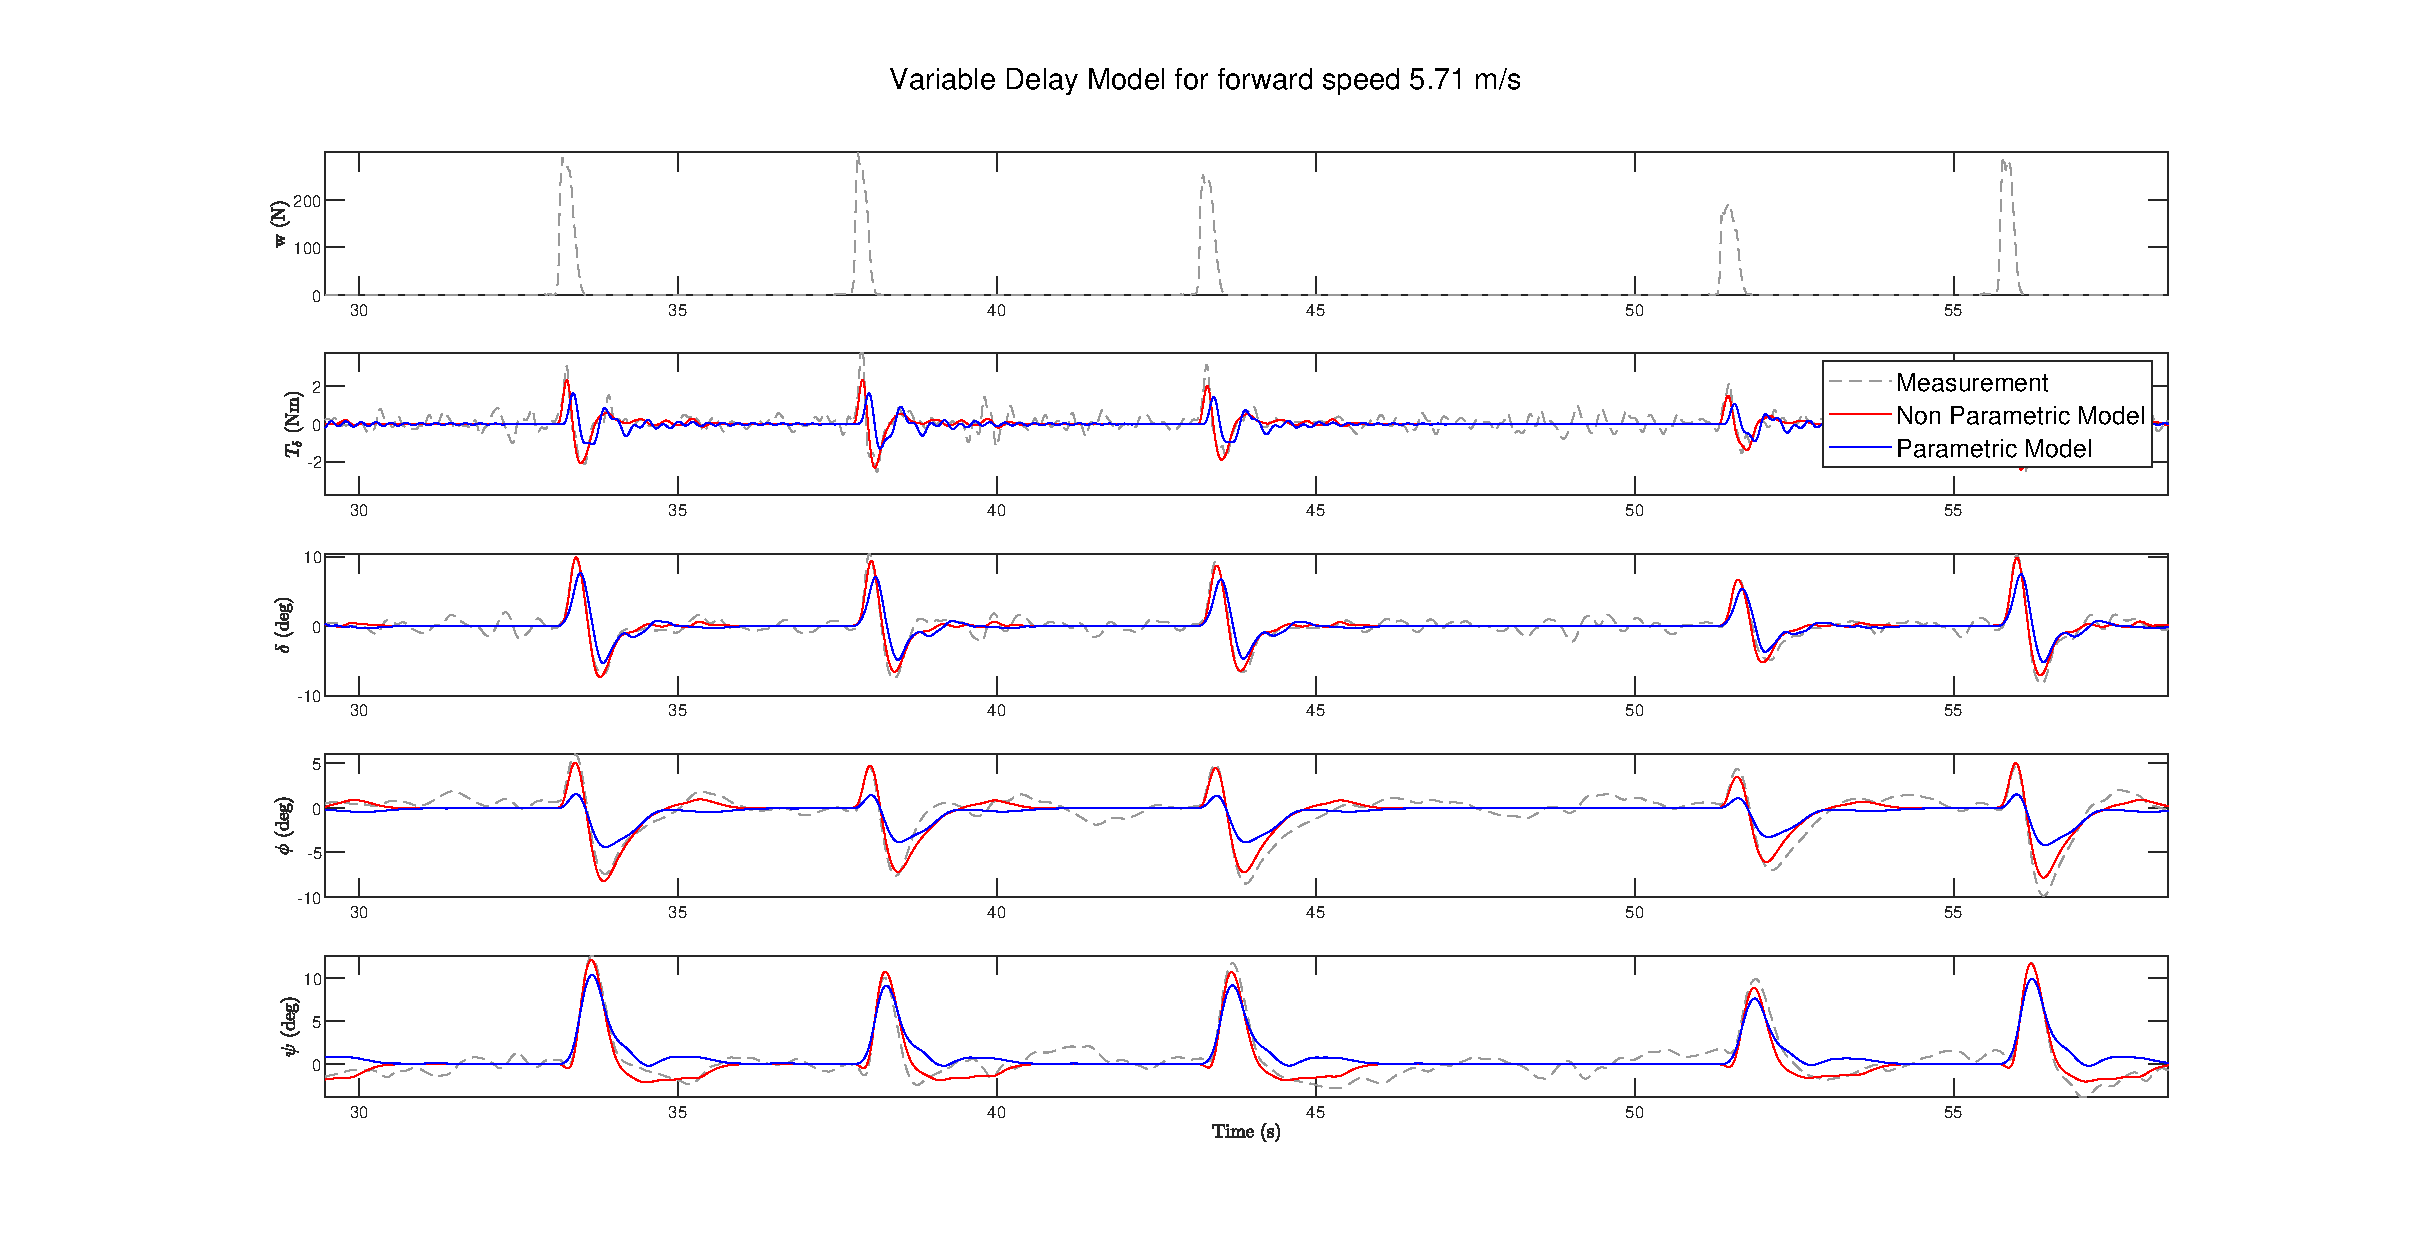
\includegraphics[width=1.4\textwidth]{images/raw_fit_plots/delay_57.eps}}
        \caption{}
        \label{fig:dm_fit4}
    \end{subfigure}
    
    \caption{Comparison between parametric model output (Variable Delay Model), non-parametric model output and measured signals for the two highest speed levels for the case where torque feedback is present in the rider control model and bicycle is operating under the "haptics on" dynamics.}
    \label{fig:dm_fitB}
 \end{figure}

\begin{figure}[!h]
    \centering
    \captionsetup{justification=centering,margin=2cm}

    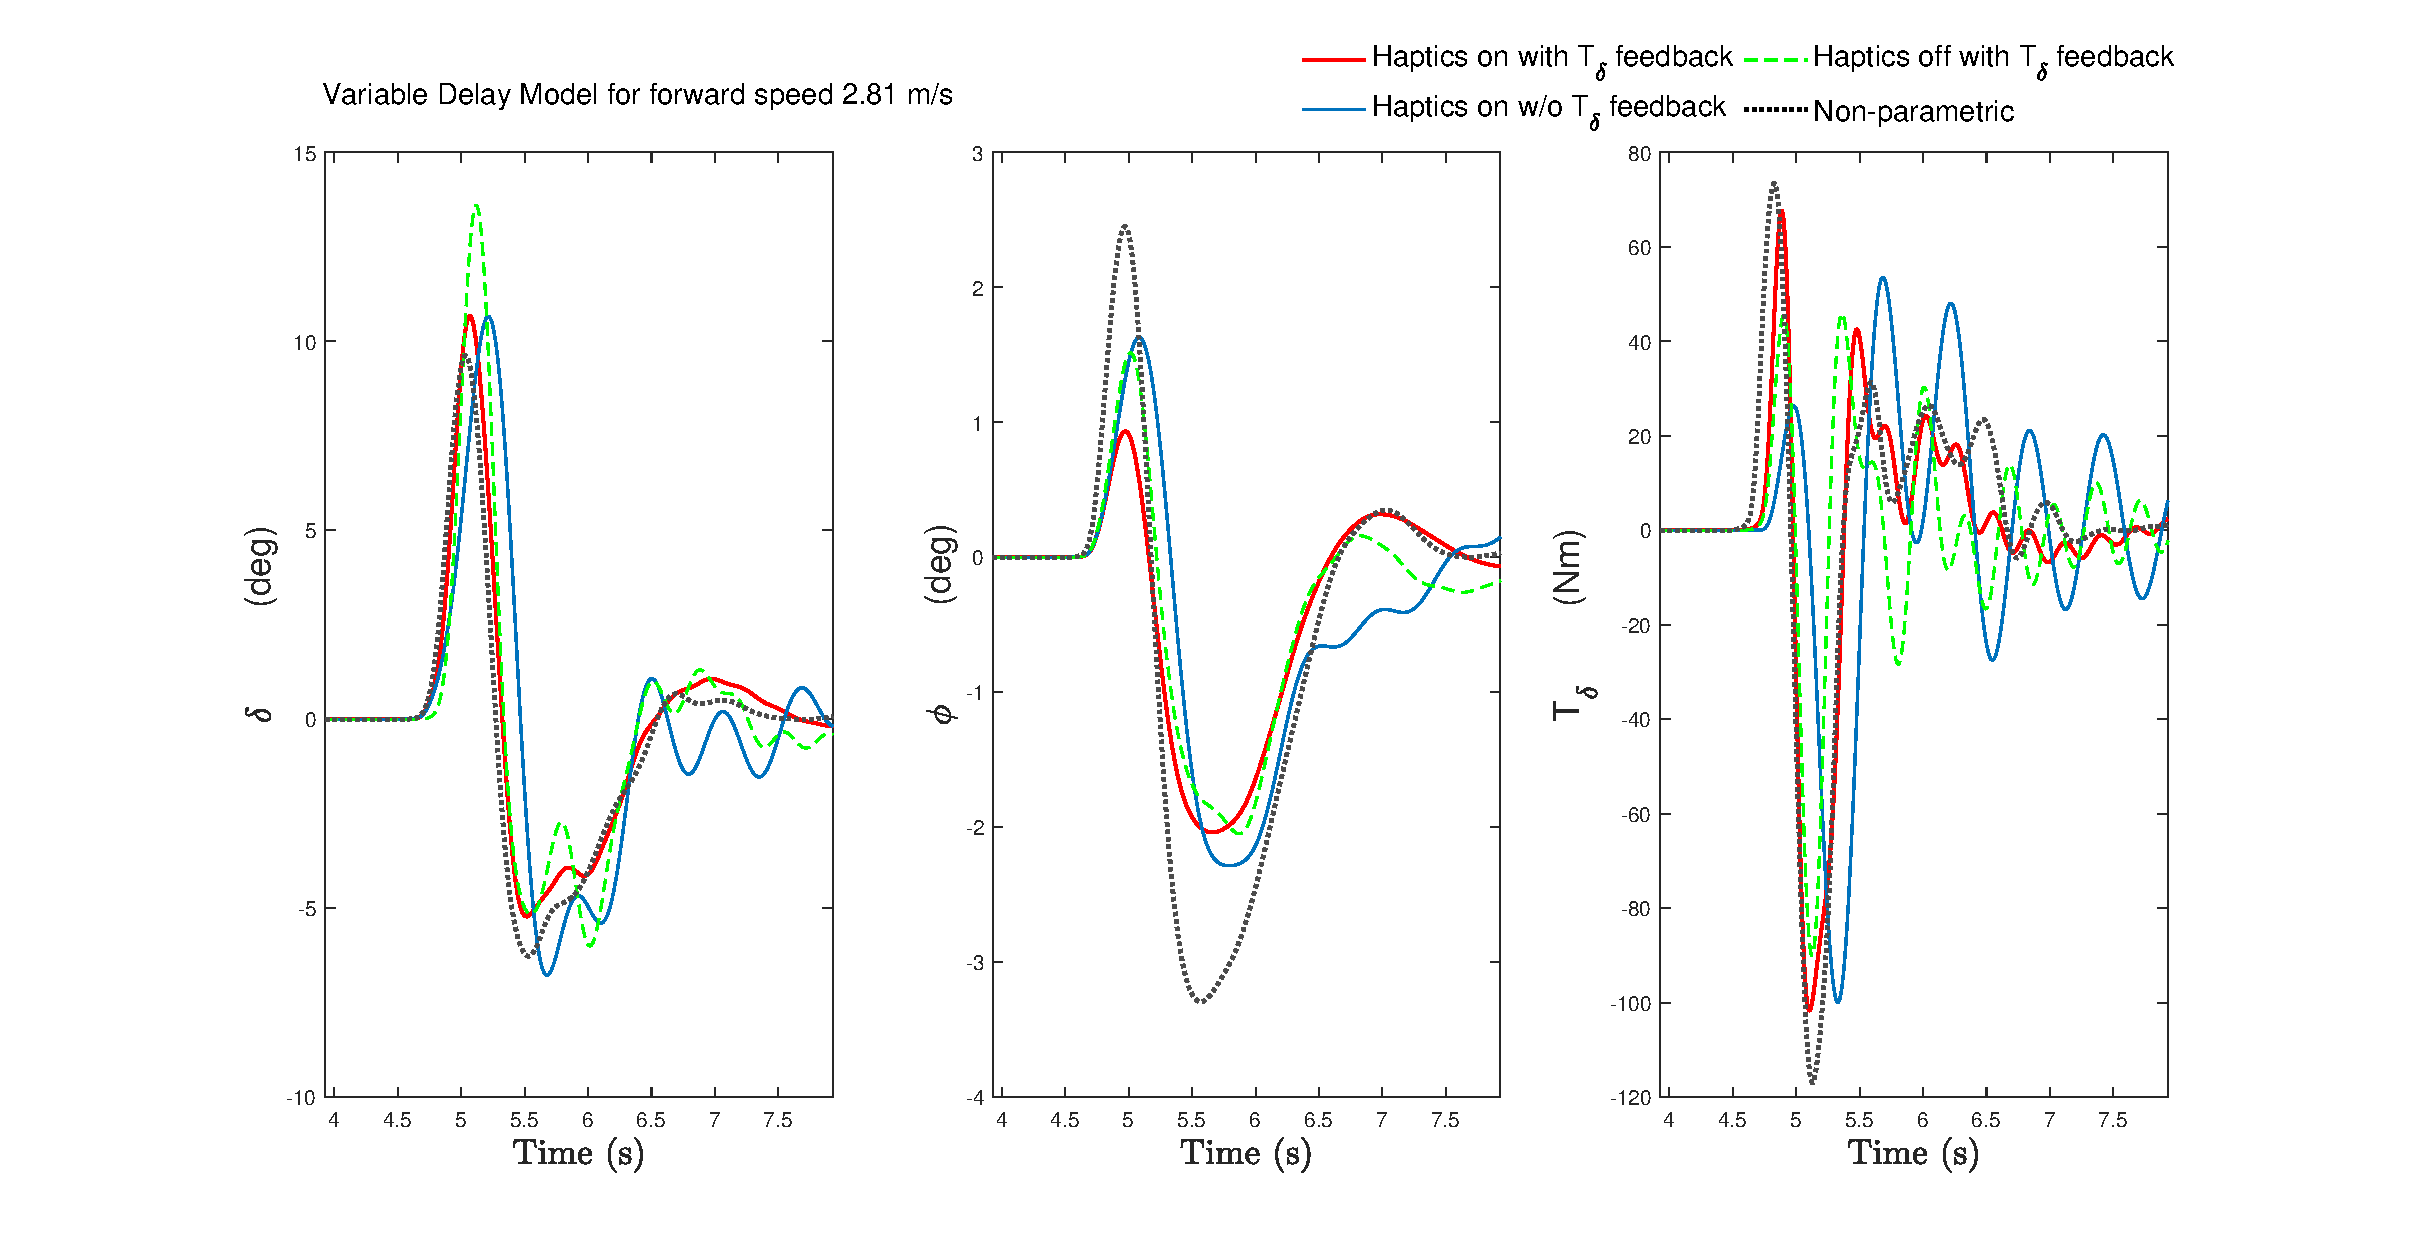
\includegraphics[width=\textwidth]{images/fb_compare_plots/delay_fb_compare28.eps}
    \caption{Steering, roll angle and input rider torque of the median rider compared among torque feedback levels  for the forward speed of 2.81 \si{\meter\per\second} in the Variable Delay Model. Response of the first disturbance in the run is shown.}
    \label{fig:paper8}
\end{figure}


\subsection{Variable Delay Reafferent Optimal Prediction  Model}

The VDROP model of  \cref{fig:paper4} is implemented with a variable  time delay among sensory pathways equal to the values used in the variable delay model. It is assumed that the internal model of bicycle and neuromuscular dynamics along with the internal model of the inherent time delay responsible for prediction is perfect for controlling the normal bicycle dynamics (\ensuremath{A^*=A_m^*}). However in the haptics off case, where the steering dynamics change, the internal model is not updated in simulation on purpose. This falls inline with what was noted during the experiments where the subjects adapted to the new bicycle dynamics instantaneously, so a full "re-calibration" of the forward model is too far fetched. This way the extent to which the smith prediction principle can counter forward model inaccuracies is also tested. 


The optimization results for the VDROP model are presented in \cref{tb:predict} for the median rider. From the \ensuremath{\mathit{VAF}s} and the signals shown in \cref{fig:ropm_fitA,fig:ropm_fitB} it is visible that the quality of the fit is comparable with the ideal zero delay case. In the haptics on with \ensuremath{{T_\delta}} feedback condition \ensuremath{K_{\dot{\delta}}} shows disproportionately higher CV which indicates lower importance for the fit for the steering rate feedback. However, in the haptics on without \ensuremath{ {T_\delta}} feedback case, the gain \ensuremath{K_{\delta}} shows the highest  uncertainty (see \cref{tb:predict}). Similar drop in \ensuremath{\mathit{VAF}_\delta} is present as in the zero delay model when  \ensuremath{{T_\delta}} feedback is turned off, which shows significant importance of the golgi tendon organ sensory pathway. Furthermore, the steering response exhibits  the same oscillatory behavior when torque feedback is completely disabled (see \cref{fig:paper10} ). However, the predictor manages to compensate in the haptics off case and achieve good fit which is not present in the variable delay model(see \cref{tb:predict}). In \cref{fig:gains_speed} the gains estimated for the median rider as a function of speed for all torque feedback conditions are presented. Consistent trends could only be discerned for the heading  gain \ensuremath{K_\psi}.

\begin{figure}[!h]
    \centering
    \begin{subfigure}[b]{\textwidth}
        \centering
        \makebox[\textwidth][c]{ 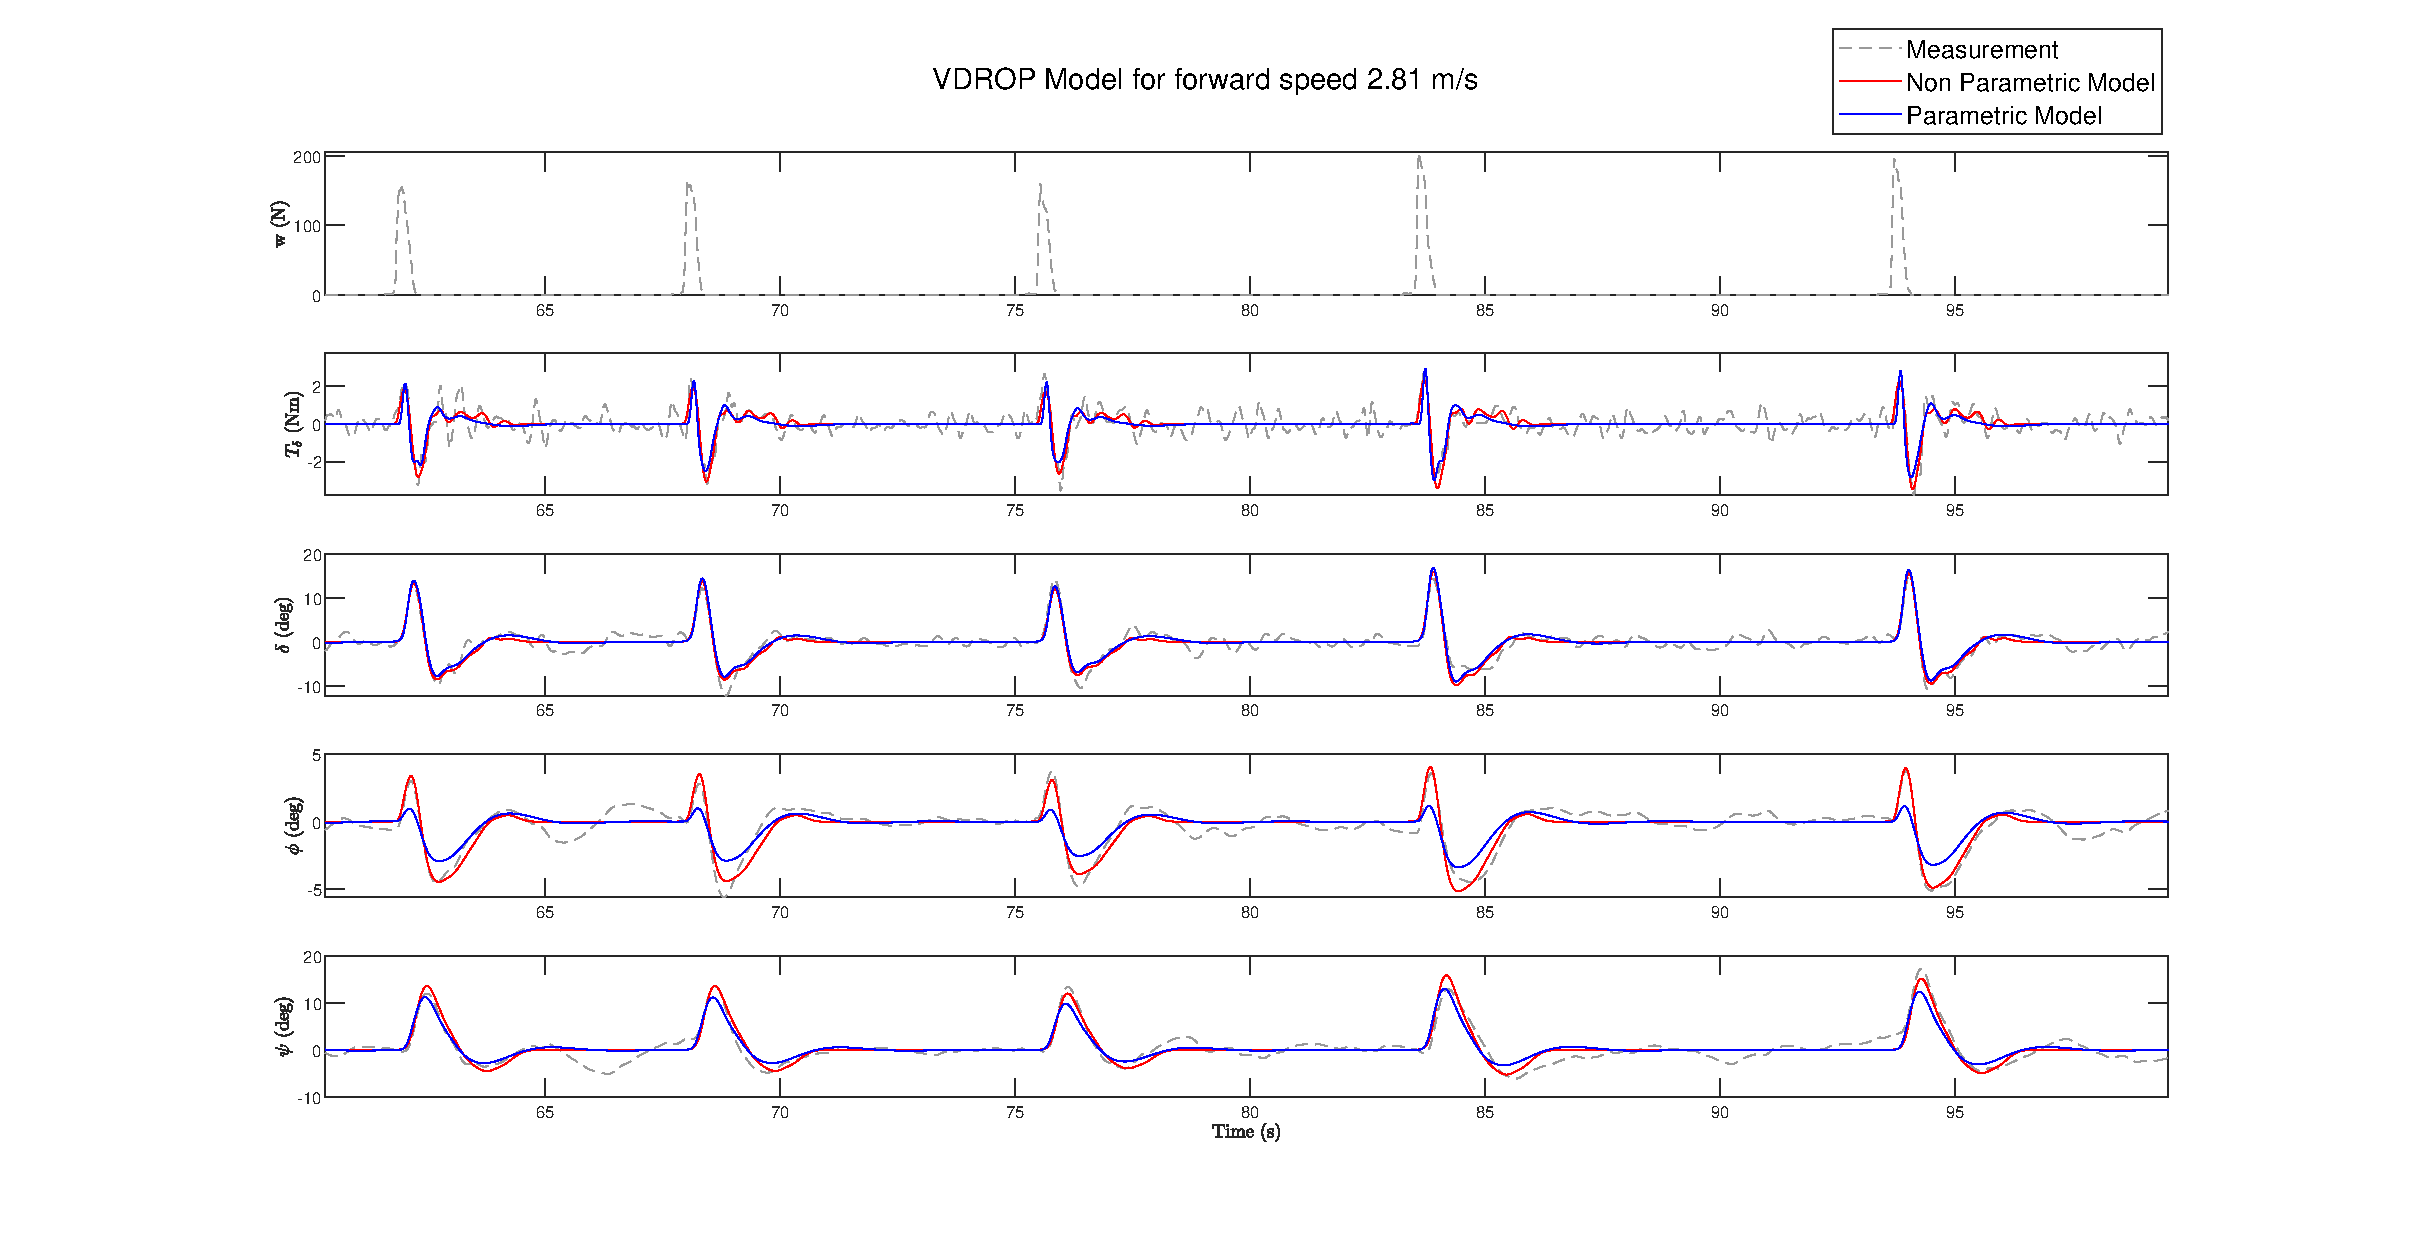
\includegraphics[width=1.4\textwidth]{images/raw_fit_plots/predict_28.eps}}
        \caption{}
        \label{fig:ropm_fit1}
    \end{subfigure}
    \begin{subfigure}[b]{\textwidth}
        \centering
        \makebox[\textwidth][c]{ 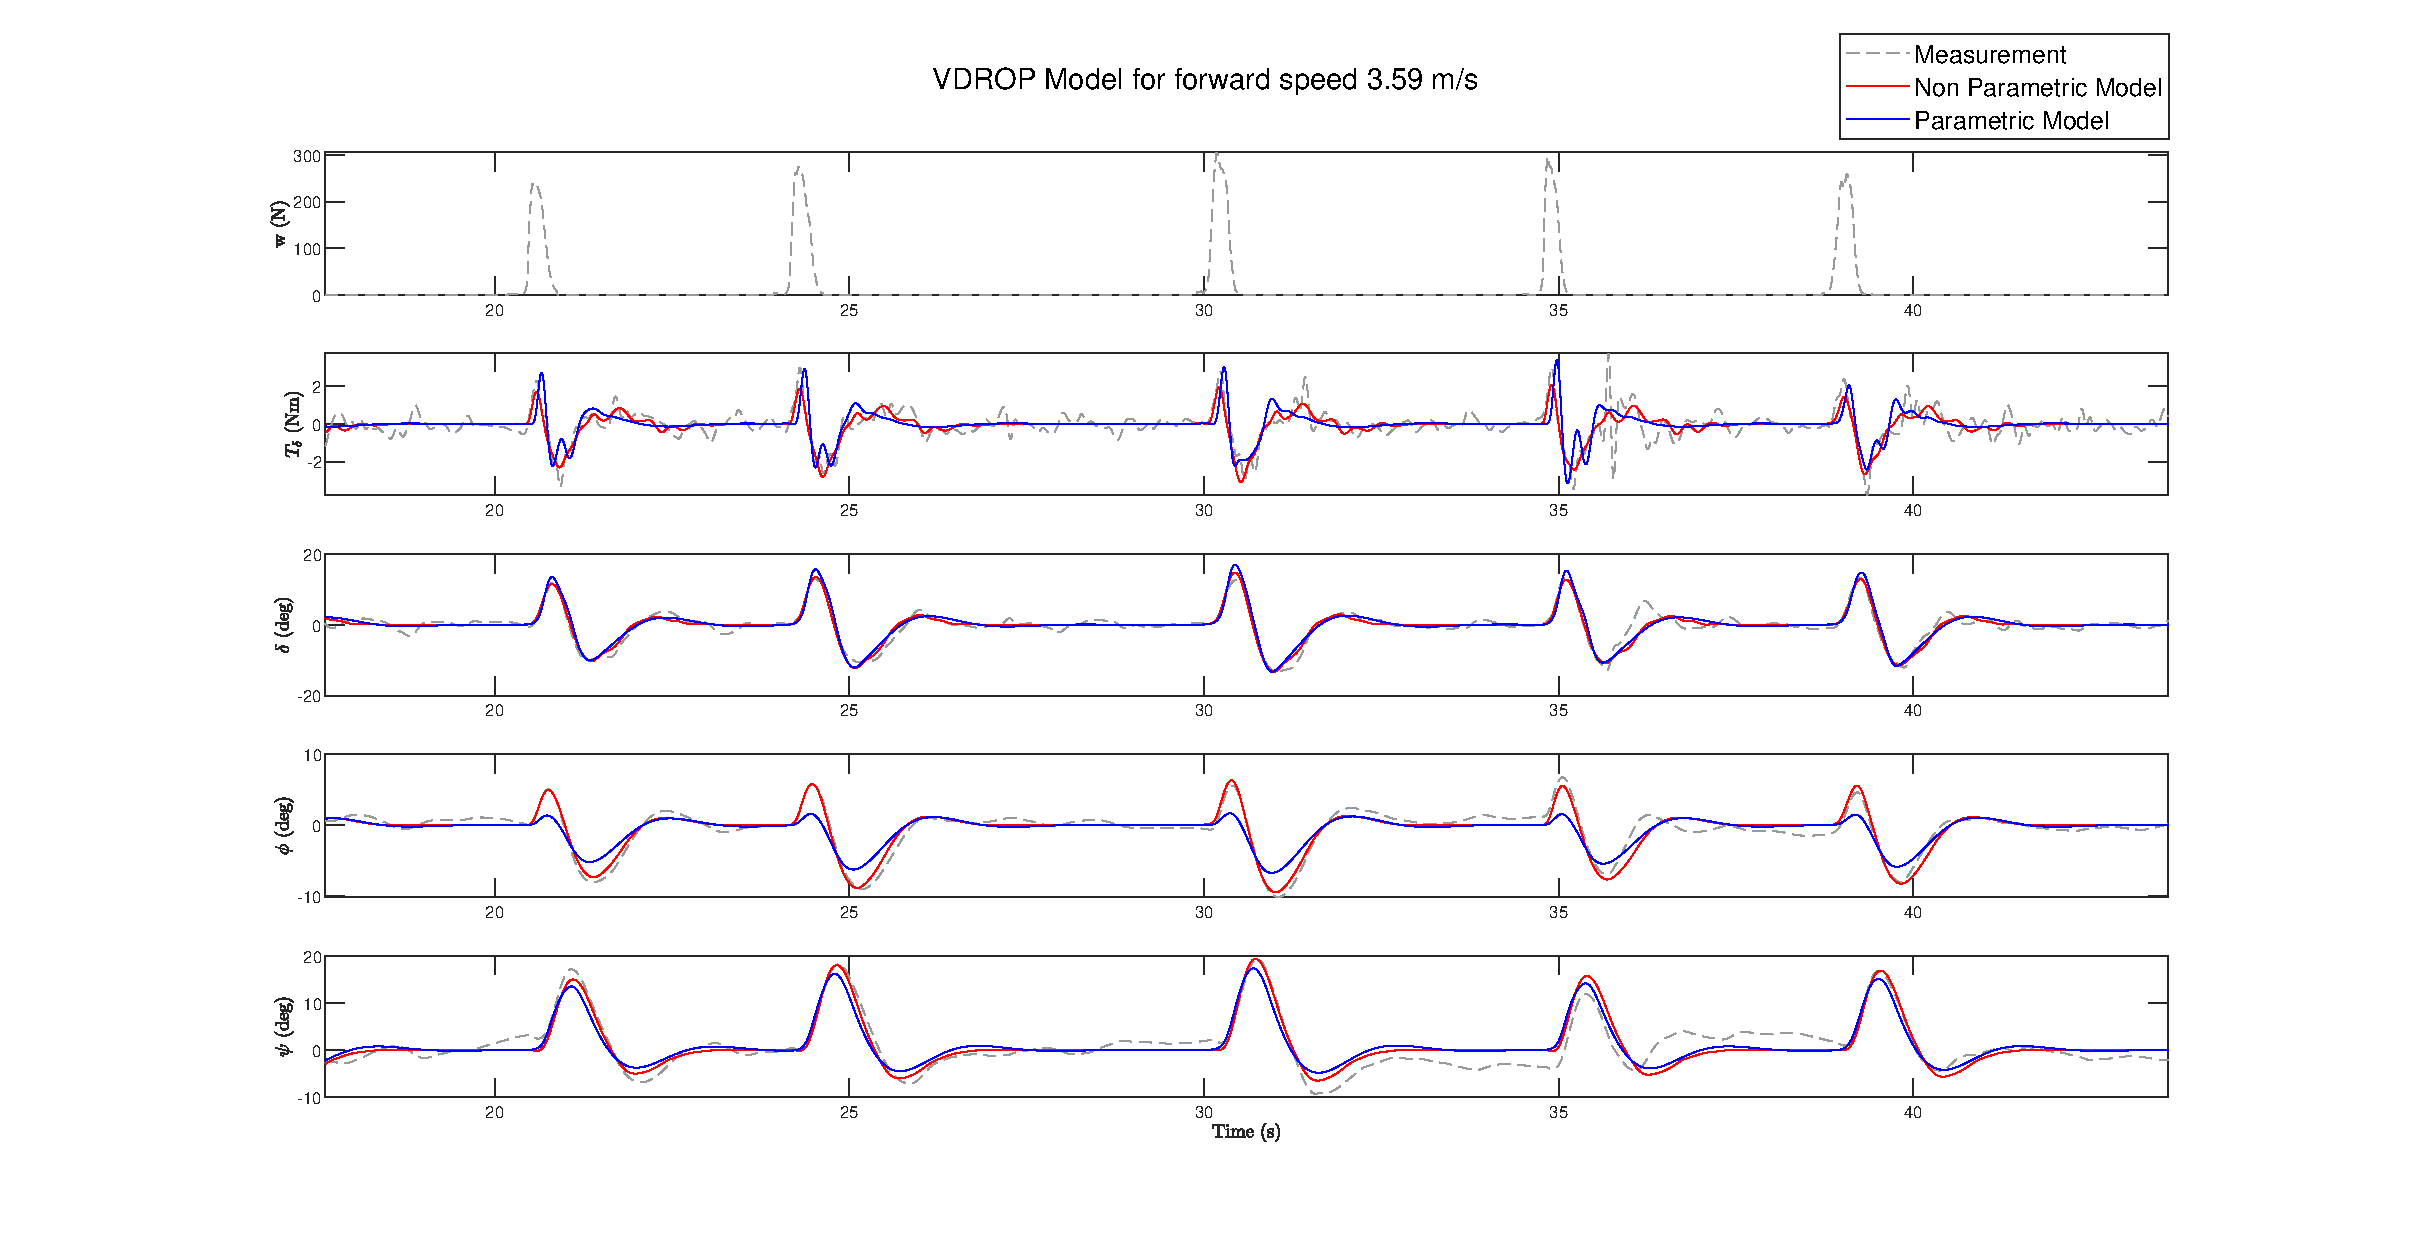
\includegraphics[width=1.4\textwidth]{images/raw_fit_plots/predict_36.eps}}
        \caption{}
        \label{fig:ropm_fit2}
    \end{subfigure}
    
    \caption{Comparison between parametric model output (VDROP Model), non-parametric model ouput and measured signals for the two lowest speed levels for the case where torque feedback is present in the rider control model and biccyle is operating under the "haptics on" dynamics.}
    \label{fig:ropm_fitA}
 \end{figure}

 \begin{figure}
    \centering
    \begin{subfigure}[b]{\textwidth}
        \centering
        \makebox[\textwidth][c]{ 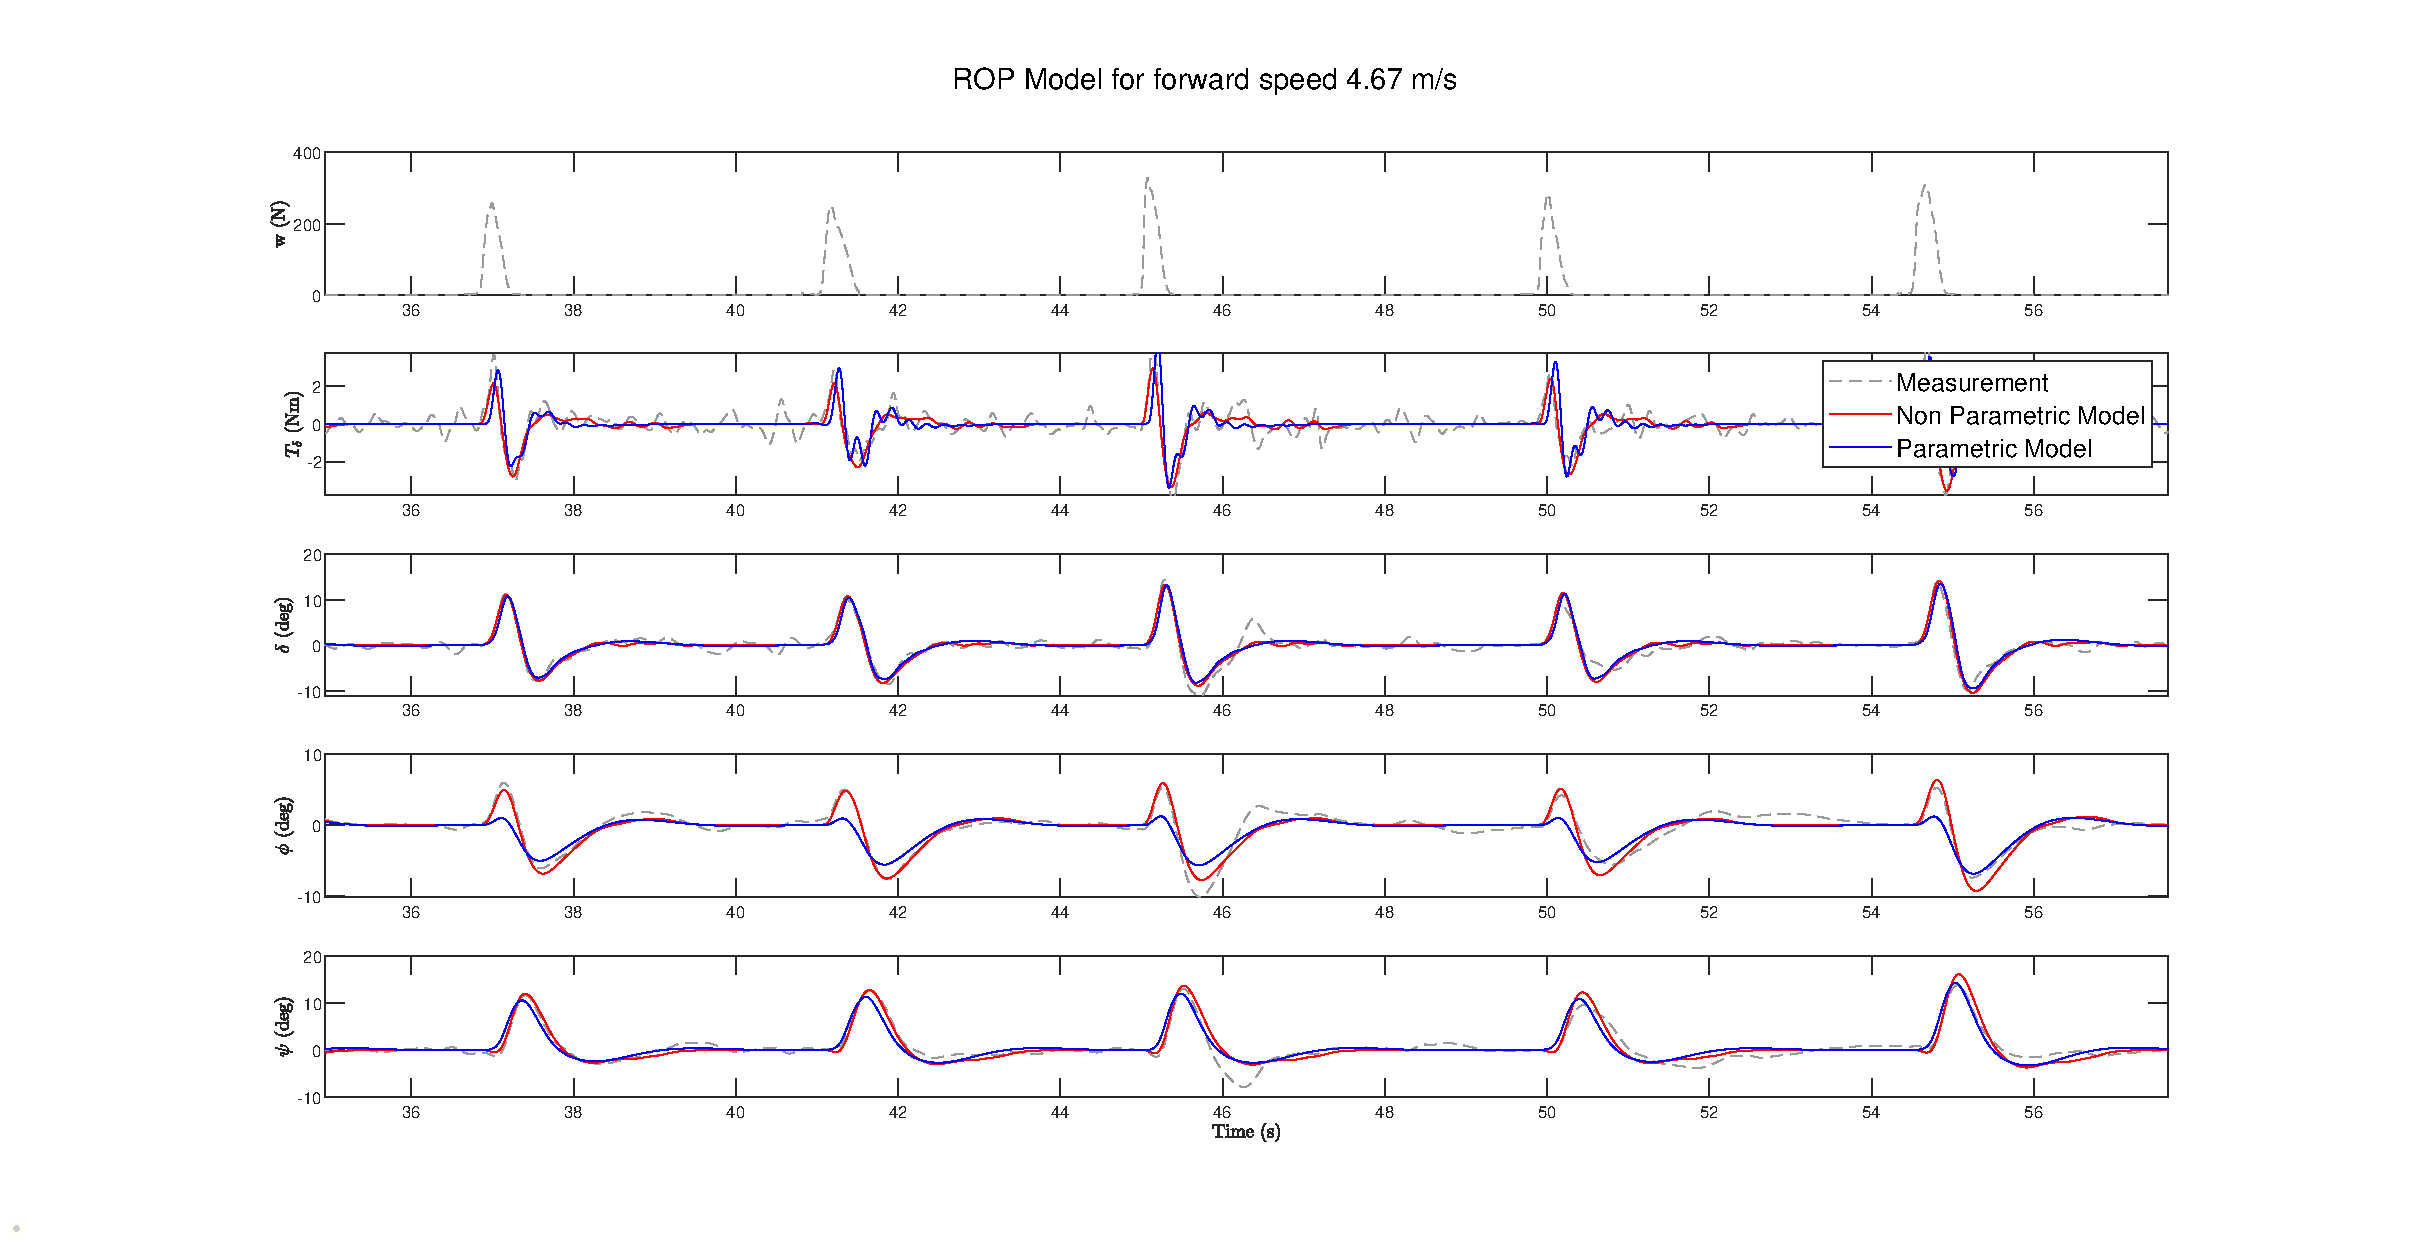
\includegraphics[width=1.4\textwidth]{images/raw_fit_plots/predict_46.eps}}
        \caption{}
        \label{fig:ropm_fit3}
    \end{subfigure}
    \begin{subfigure}[b]{\textwidth}
        \centering
        \makebox[\textwidth][c]{ 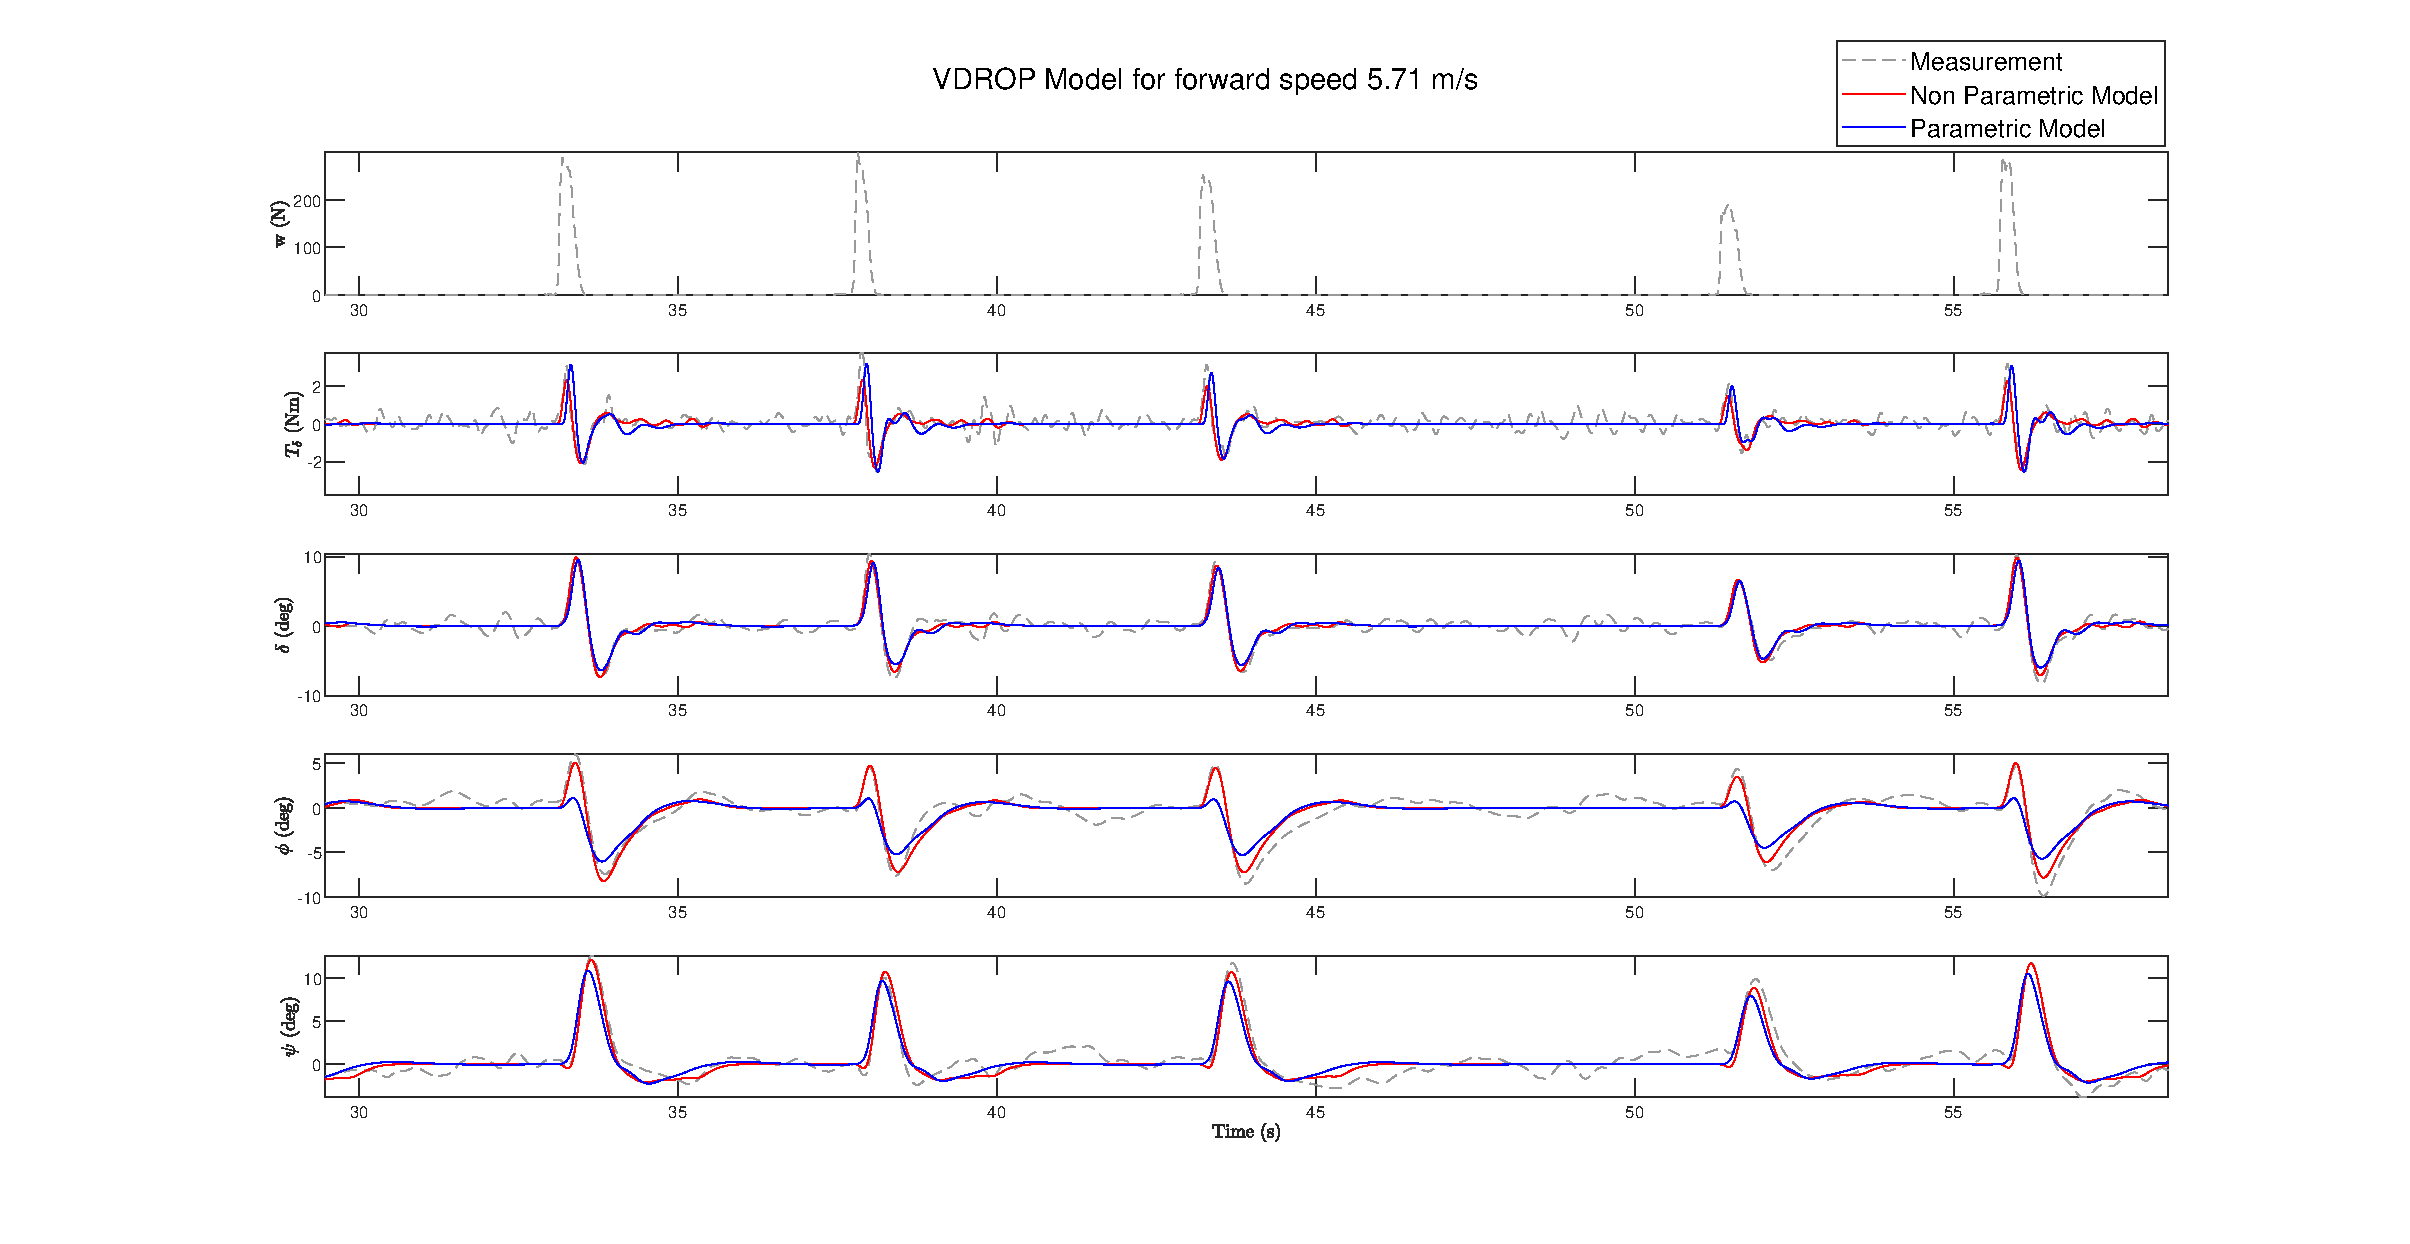
\includegraphics[width=1.4\textwidth]{images/raw_fit_plots/predict_57.eps}}
        \caption{}
        \label{fig:ropm_fit4}
    \end{subfigure}
    
    \caption{Comparison between parametric model output (VDROP Model), non-parametric model output and  measured signals for the two highest speed levels for the case where torque feedback is present in the rider control model and bicycle is operating under the "haptics on" dynamics.}
    \label{fig:ropm_fitB}
 \end{figure}


\begin{figure}[!h]
    \centering
    \captionsetup{justification=centering,margin=2cm}

    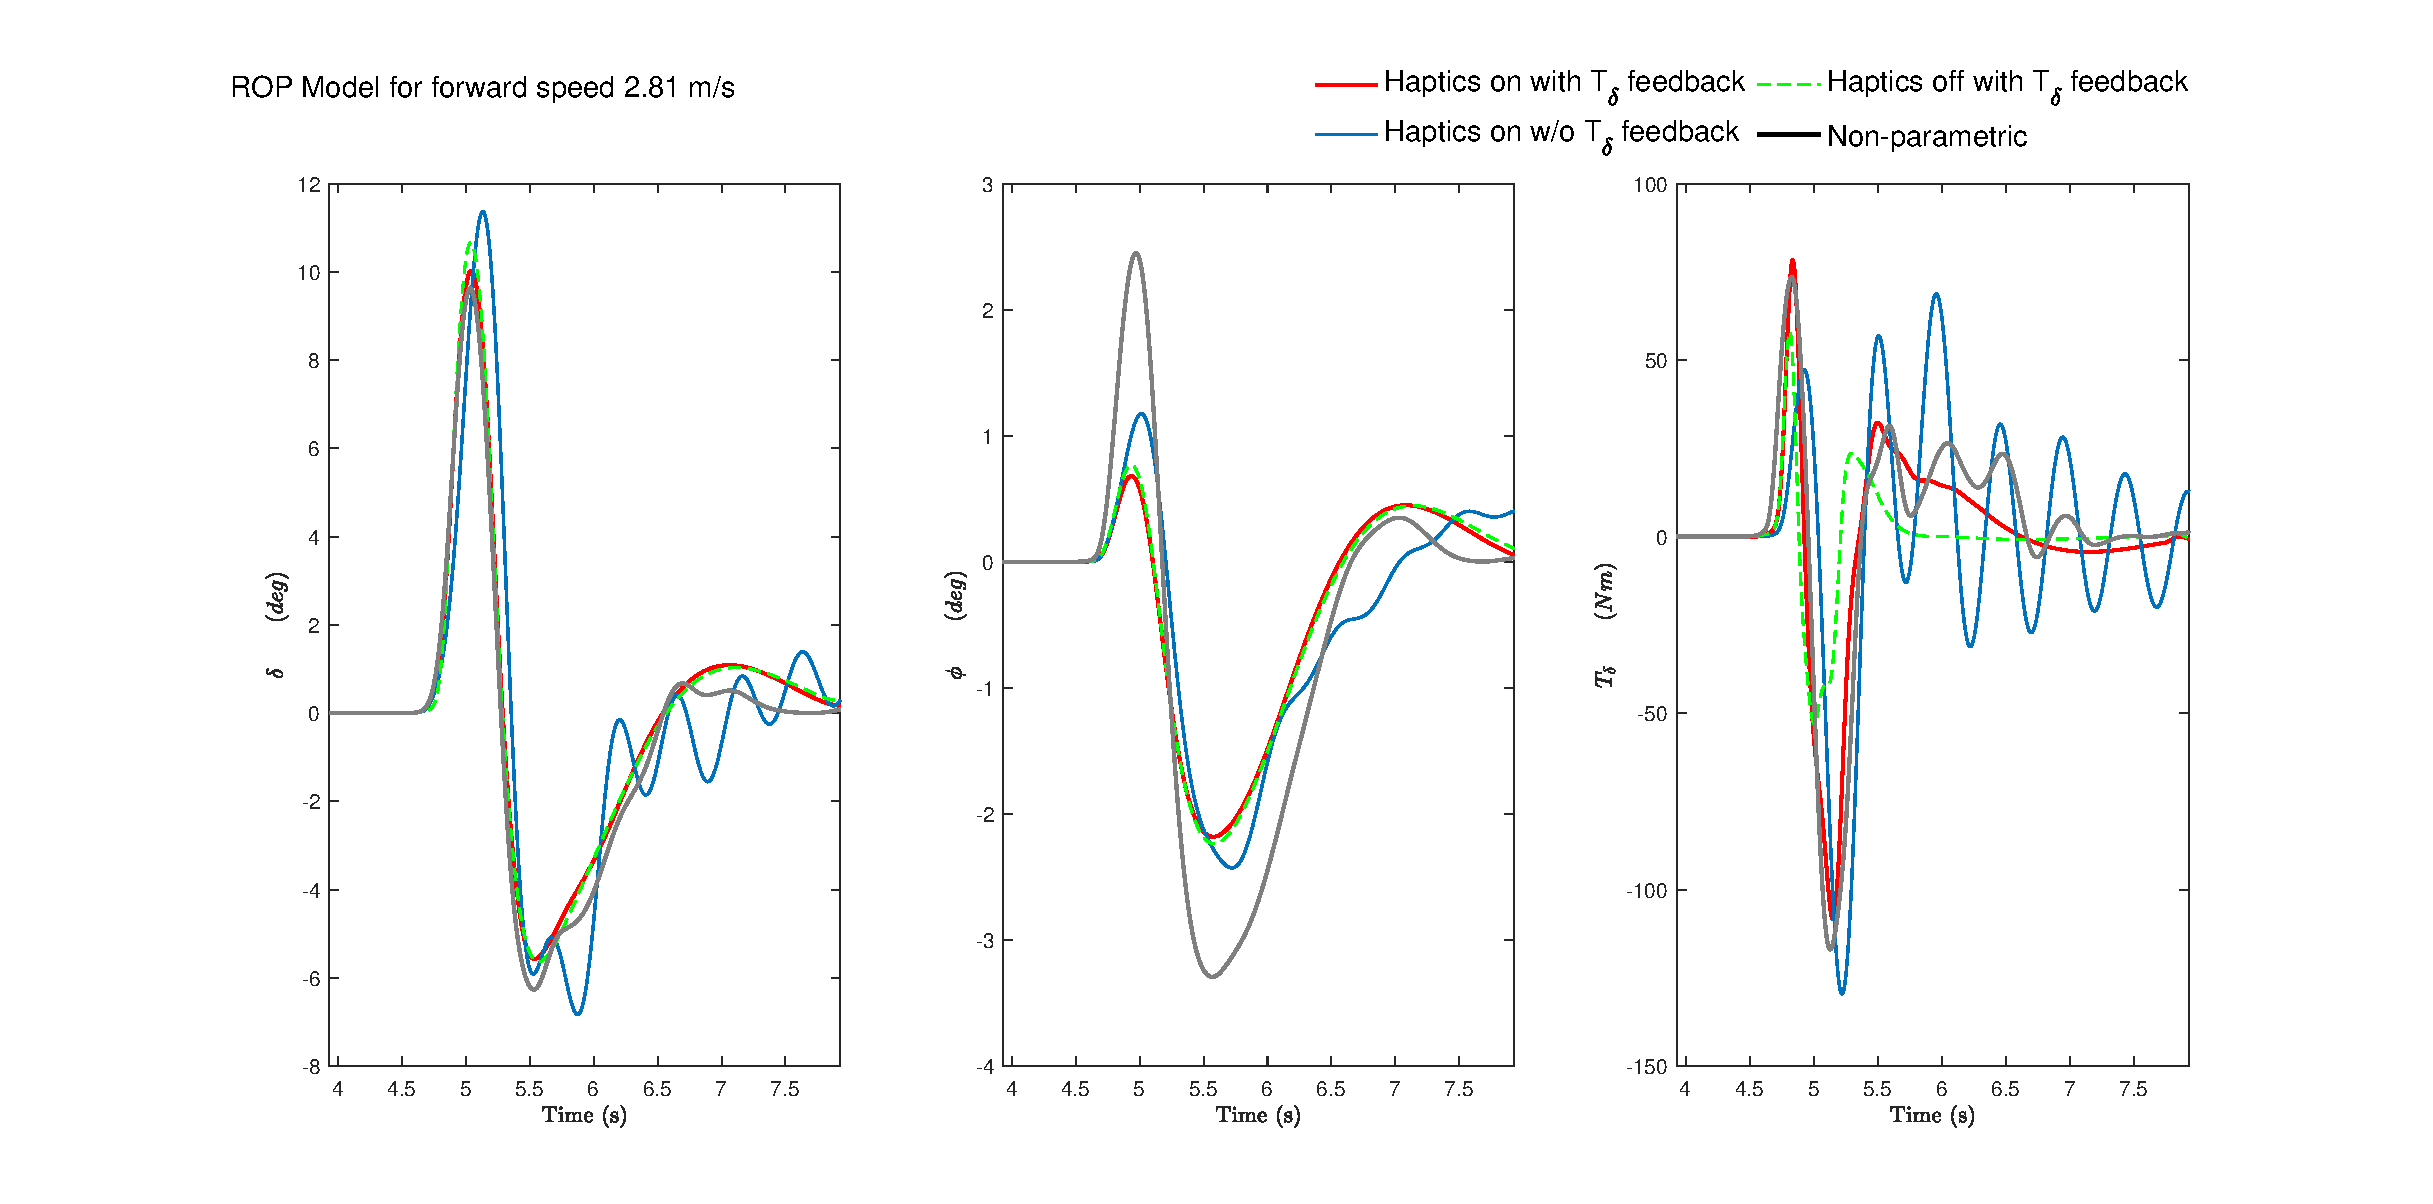
\includegraphics[width=\textwidth]{images/fb_compare_plots/ROP_fb_compare28.eps}
        \caption{Steering, roll angles and input rider torque compared among torque feedback levels  for the forward speed of 2.81 \si{\meter\per\second} in the VDROP Model. Response of the first disturbance in the run is shown.}
    \label{fig:paper10}
\end{figure}

In \crefrange{fig:results_compare12}{fig:results_compare34}  a complete comparison between rider models for all feedback conditions is presented. The response shown is the result of the first lateral perturbation of each individual run. The zero delay and prediction models exhibit almost identical responses as it was evident from the over 90\% fit achieved. The variable delay model lags behind in both the produced control input and bicycle output, as is expected. Worth noting the lag in the control input of the prediction model in the first few milliseconds after the perturbation. Despite that fact the VDROP model compensates and achieves similar output as the idealized zero delay case. This is a result of the fact that no matter how good the prediction algorithm is the human has no knowledge of the future so the response from the controller will start after the first state information arrives from the feedback pathways which are delayed. The forward model in this case does not help predict the state as it has no information of the external disturbance. 
% Please add the following required packages to your document preamble:
% \usepackage{multirow}





    \begin{figure}
        \centering
        \begin{subfigure}[b]{\textwidth}
            \centering
            \makebox[\textwidth][c]{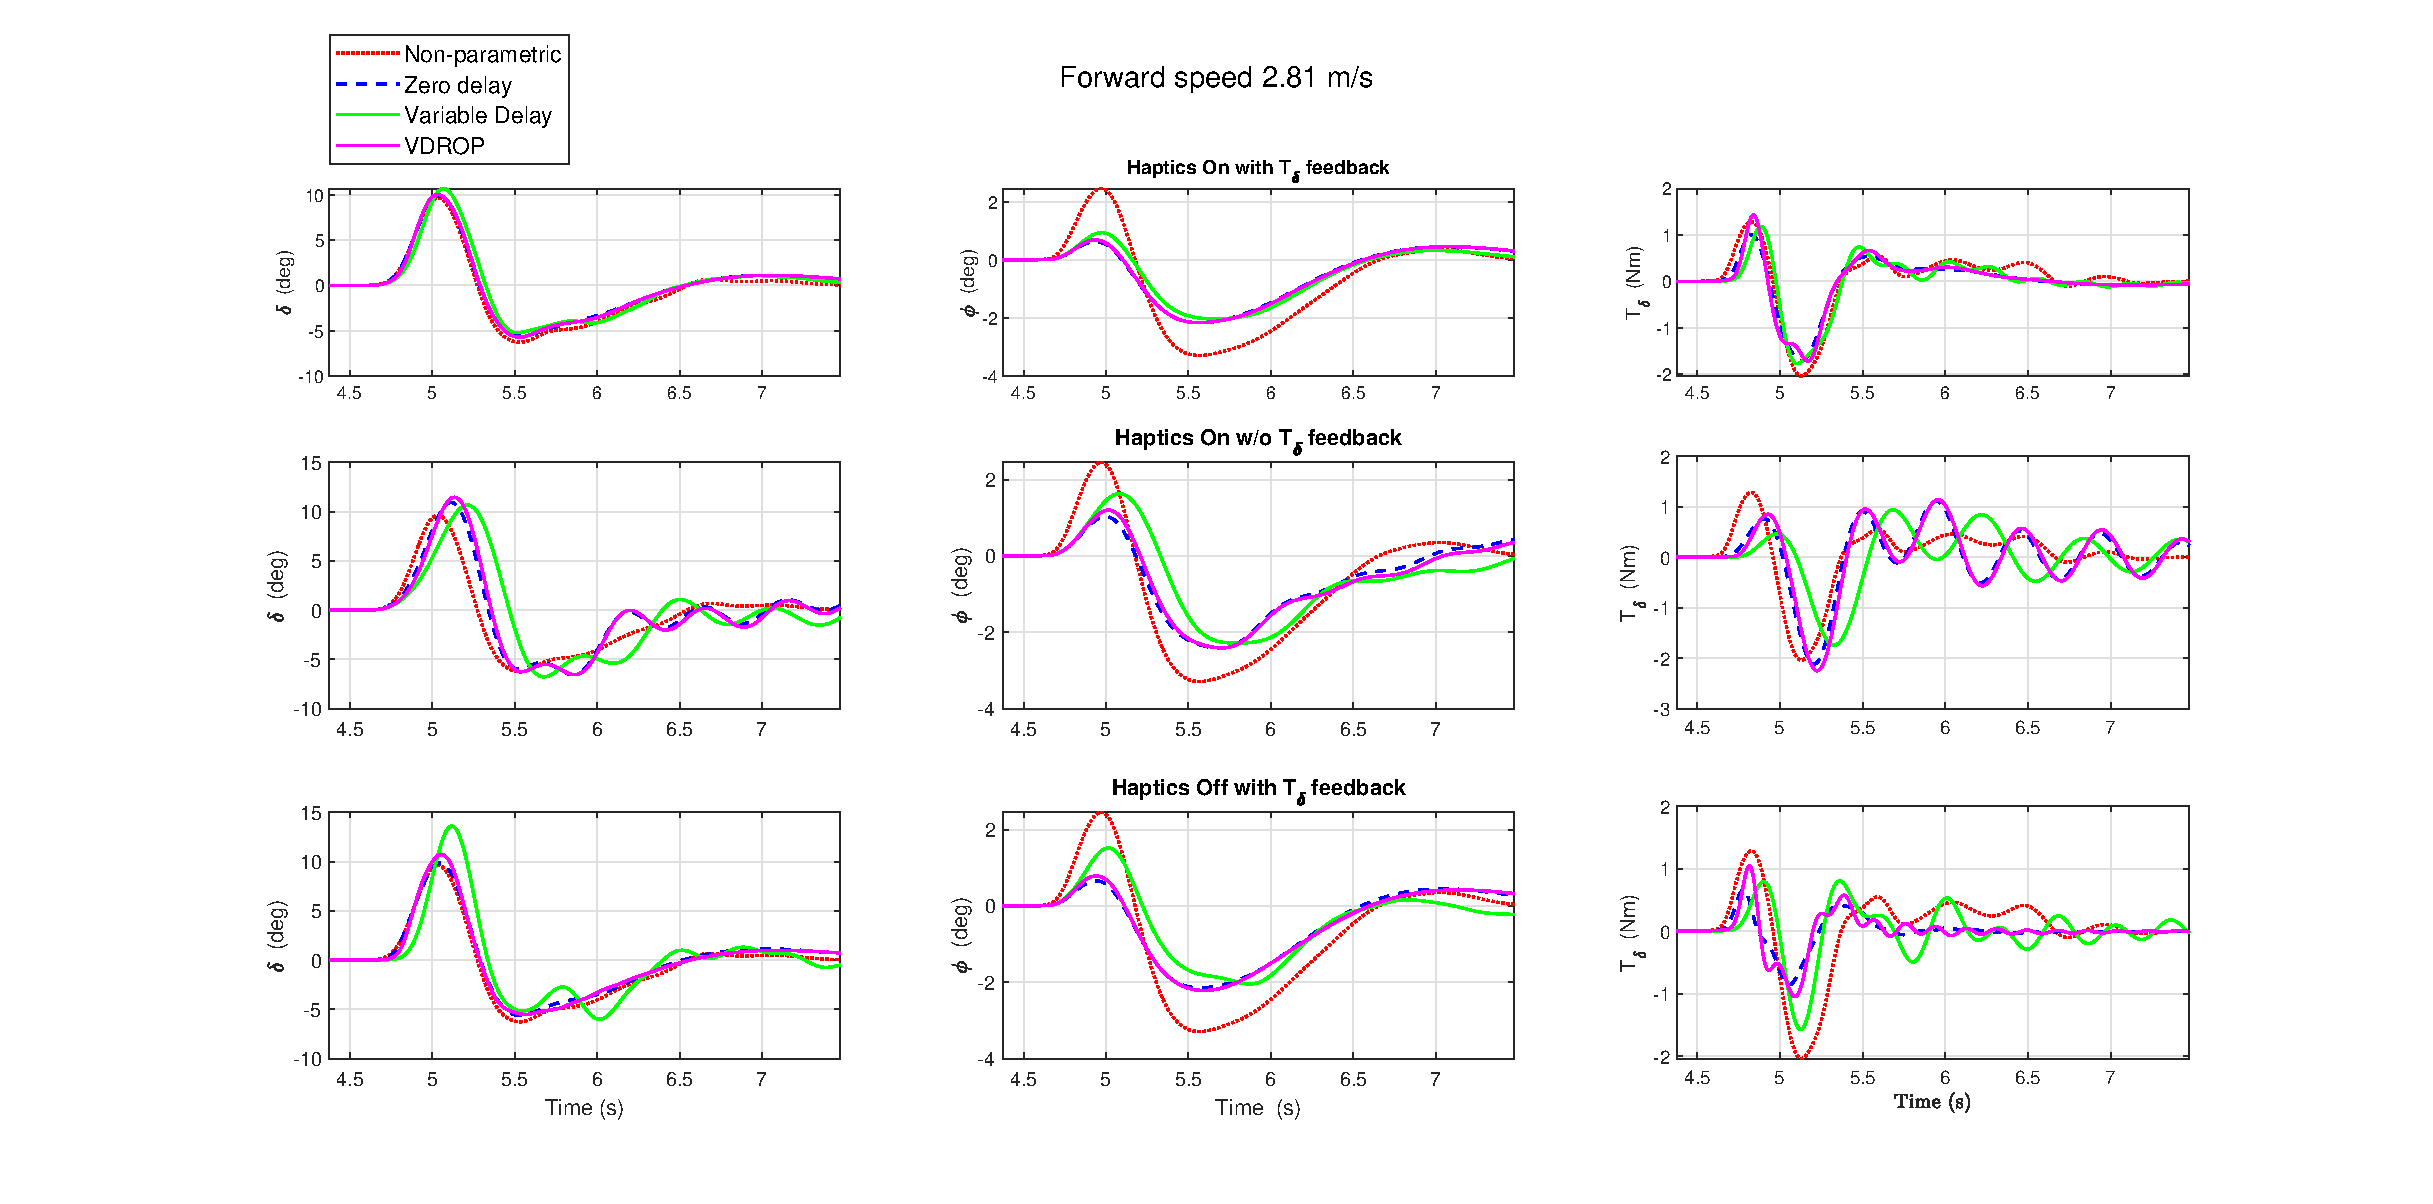
\includegraphics[width=1.4\textwidth]{images/compare_model_plots/compare_models_28.eps}}
            \caption{Comparison between the three rider models for forward speed 2.81 \si{\meter\per\second}}
            \label{fig:results_compare1}
        \end{subfigure}
        \begin{subfigure}[b]{\textwidth}
            \centering
            \makebox[\textwidth][c]{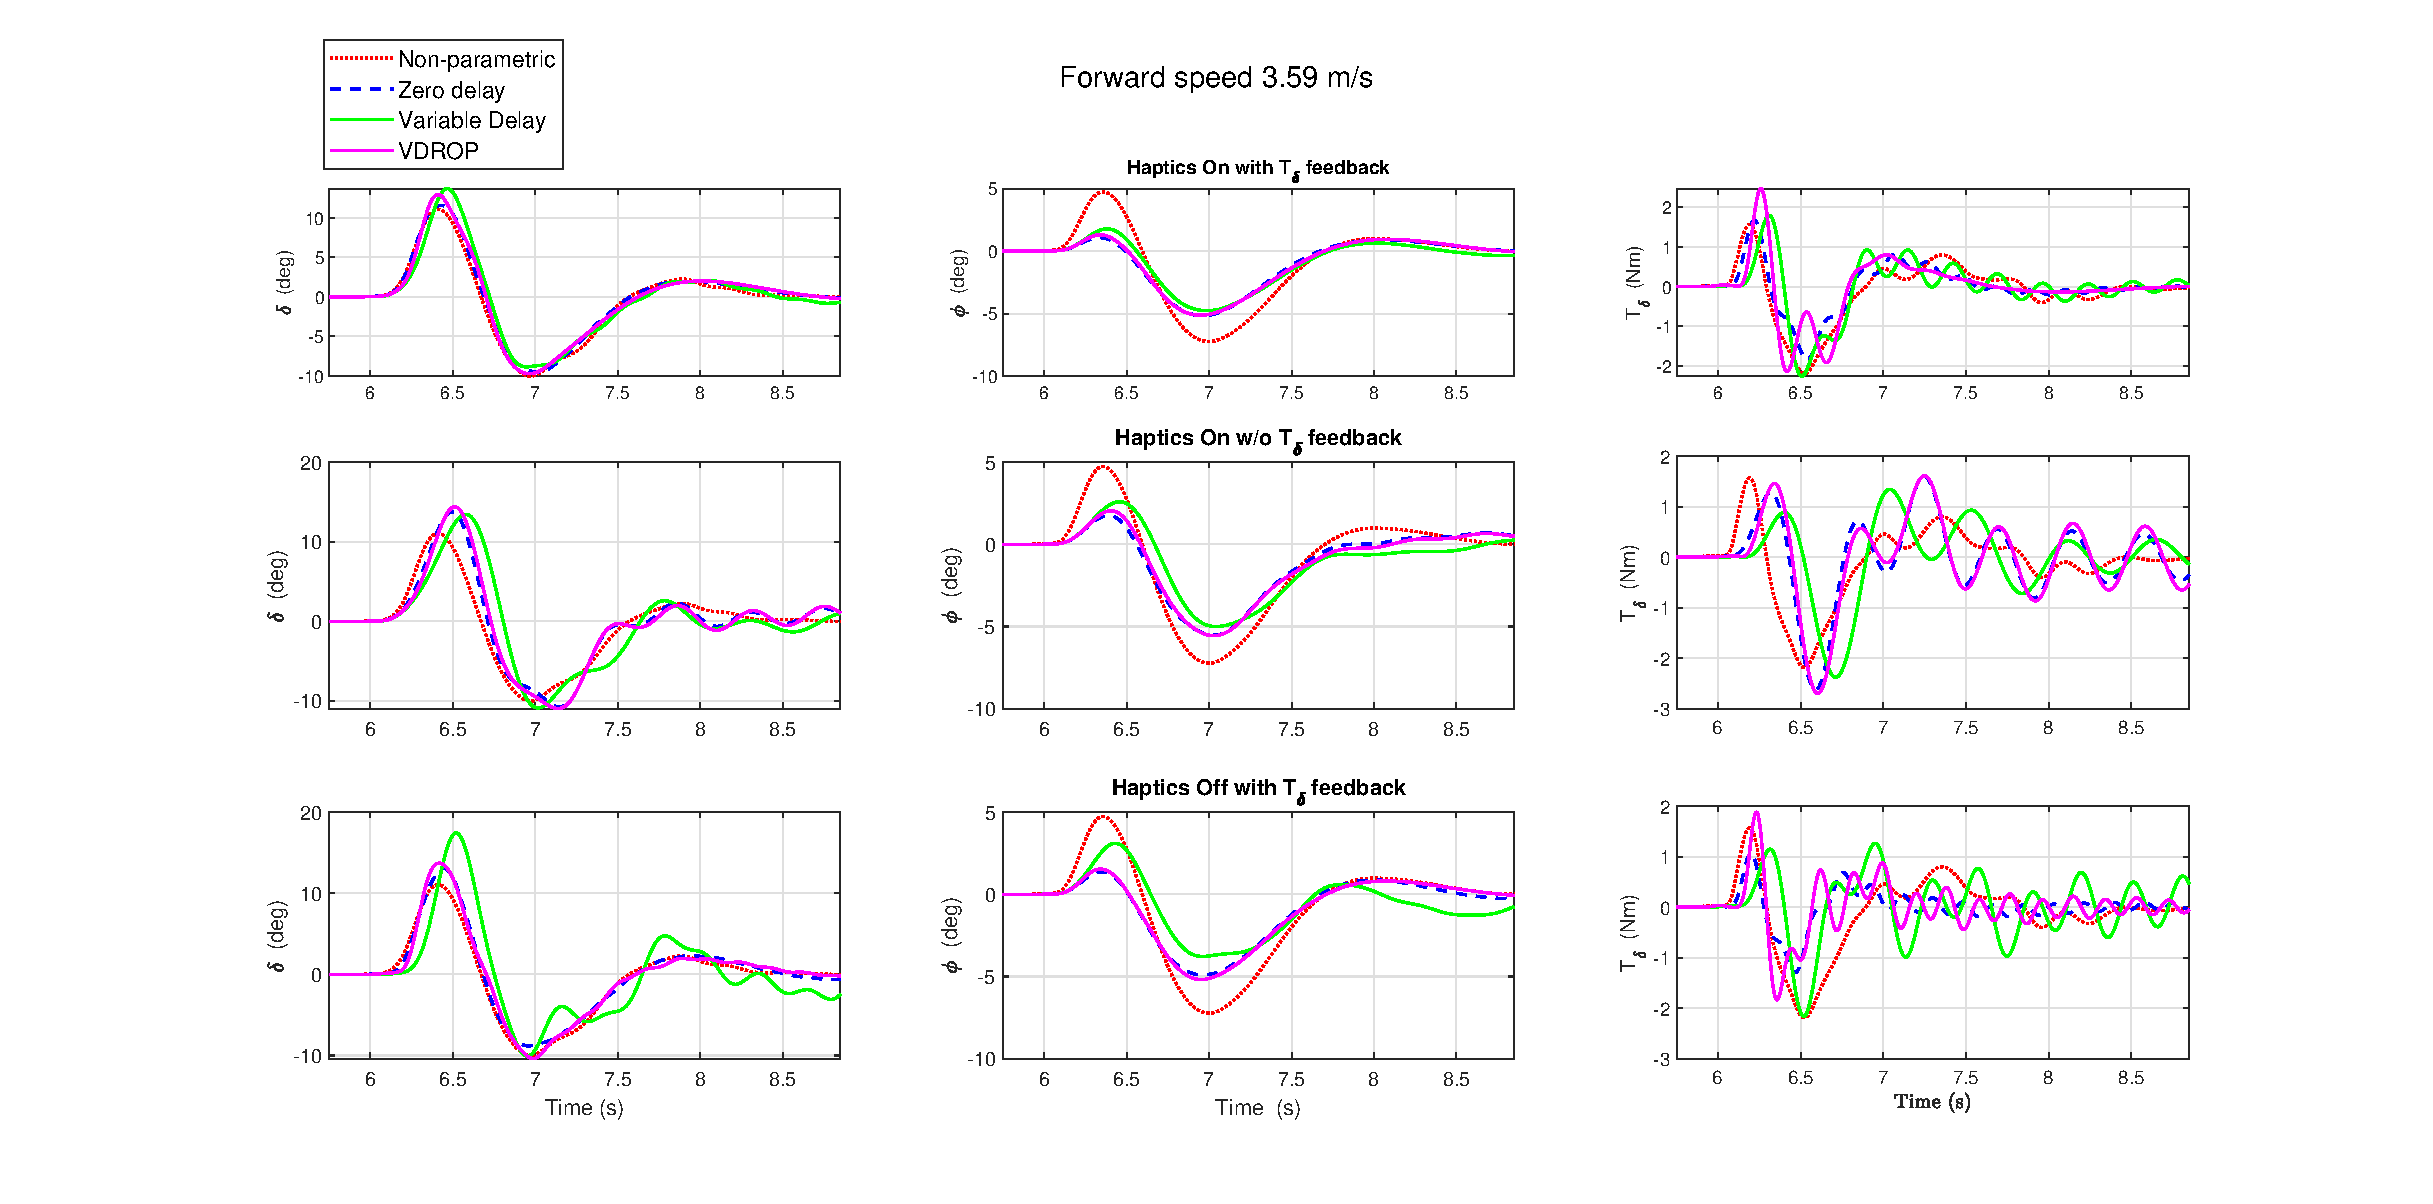
\includegraphics[width=1.4\linewidth]{images/compare_model_plots/compare_models_36.eps}}
            \caption{Comparison between the three rider models for forward speed 3.6 \si{\meter\per\second}}            
            \label{fig:results_compare2}
        \end{subfigure}
        \caption{Steering angle \ensuremath{\delta}, roll angle \ensuremath{\phi} and steering torque \ensuremath{T_\delta} compared among the three rider models implemented for all torque feedback conditions, for the two lowest speed levels for the response of the median rider to the first perturbation of each run. Non parametric output included for reference.}
        \label{fig:results_compare12}
     \end{figure}



     \begin{figure}
        \centering
        \begin{subfigure}[b]{\textwidth}
            \centering
            \makebox[\textwidth][c]{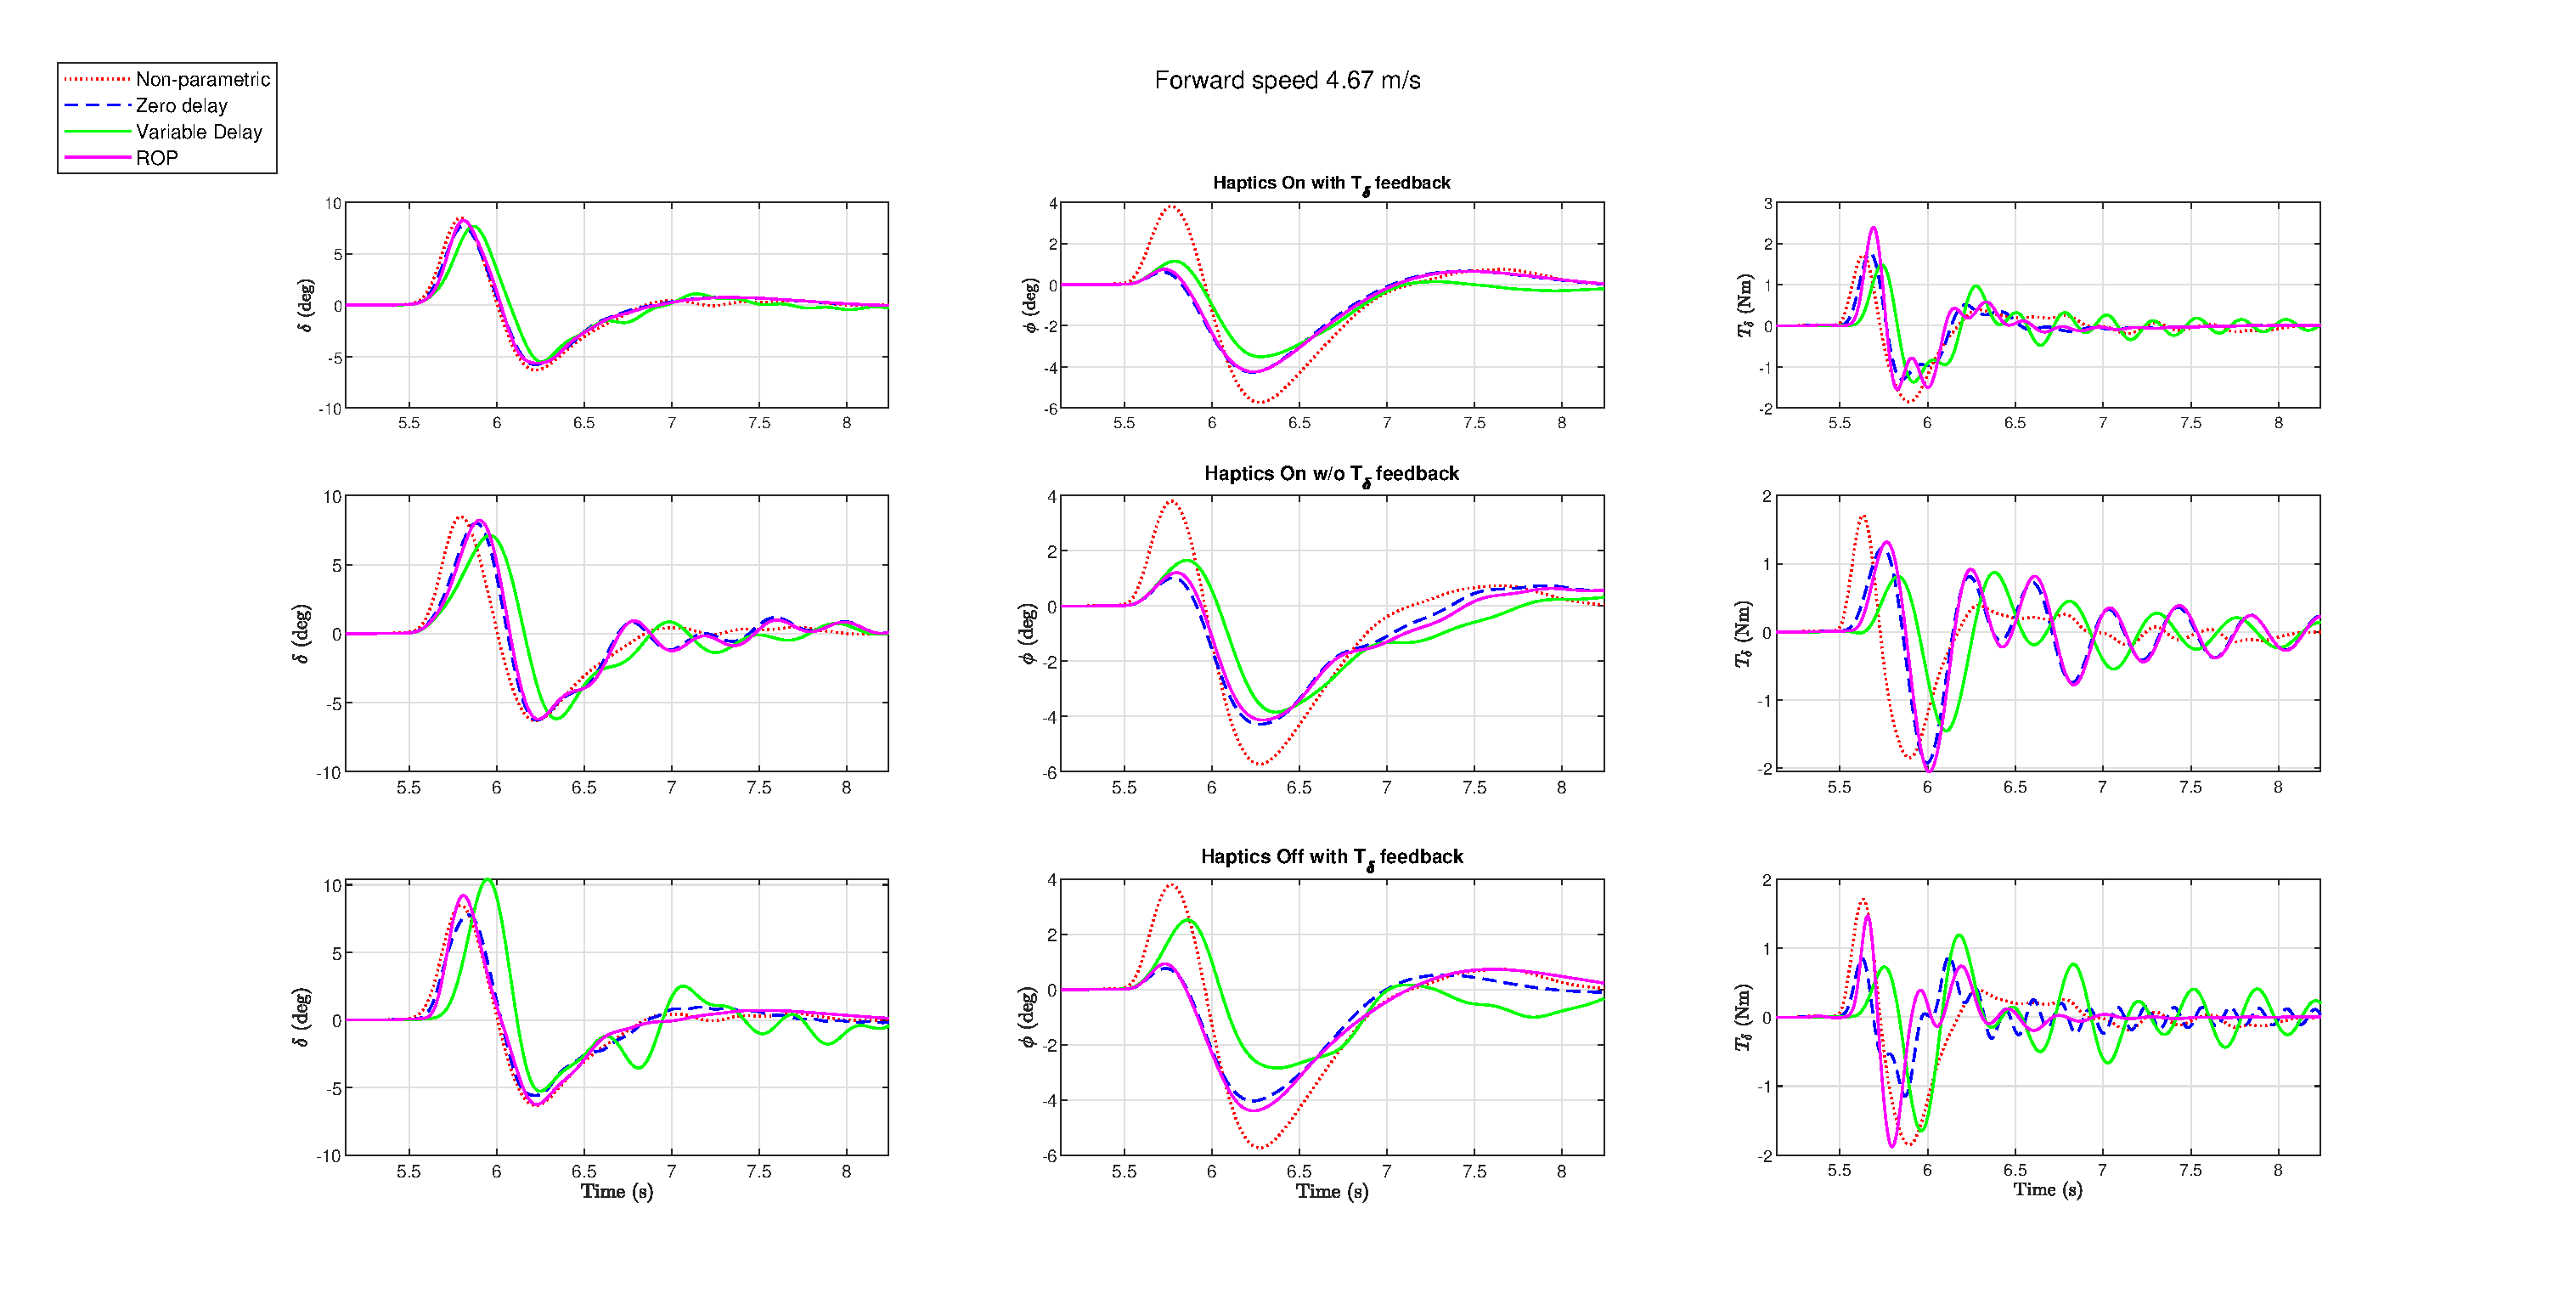
\includegraphics[width=1.4\linewidth]{images/compare_model_plots/compare_models_46.eps}}
            \caption{Comparison between the three rider models for forward speed 4.67 \si{\meter\per\second}}
            \label{fig:results_compare3}
        \end{subfigure}
        \begin{subfigure}[b]{\textwidth}
            \centering
            \makebox[\textwidth][c]{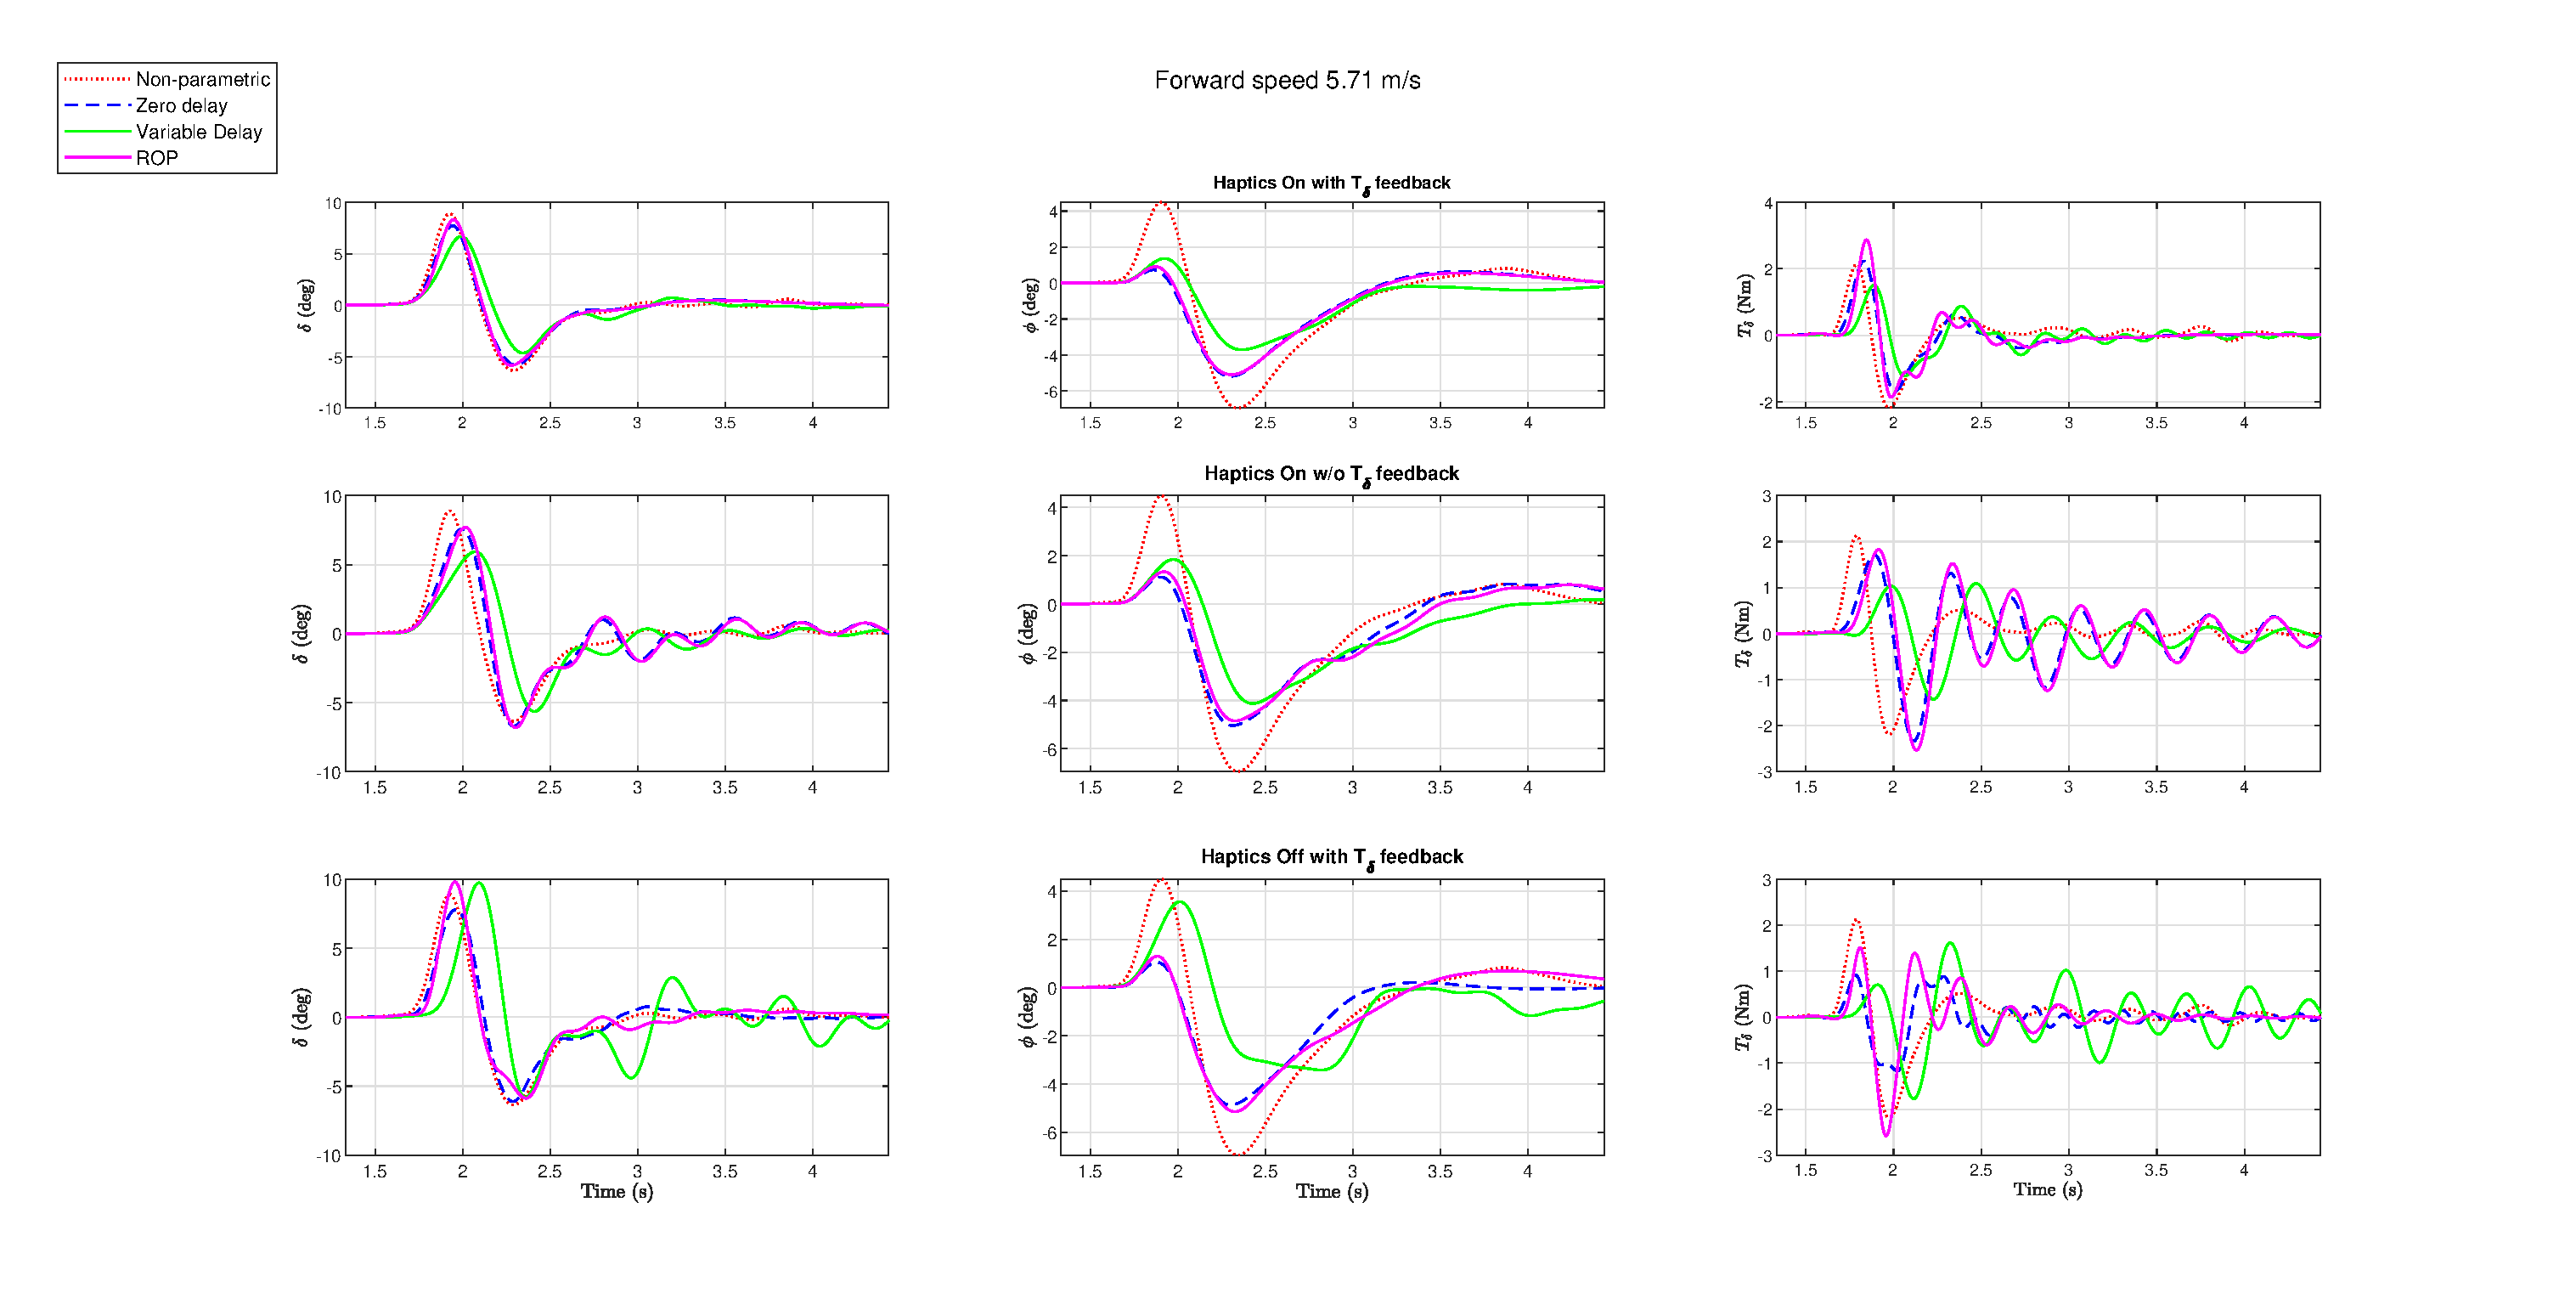
\includegraphics[width=1.4\linewidth]{images/compare_model_plots/compare_models_57.eps}}
            \caption{Comparison between the three rider models for forward speed 5.71 \si{\meter\per\second}}            
            \label{fig:results_compare4}
        \end{subfigure}
        \caption{Steering angle \ensuremath{\delta}, roll angle \ensuremath{\phi} and steering torque \ensuremath{T_\delta} compared among the three rider models implemented for all torque feedback conditions, for the two highest speed levels for the response of the median rider to the first perturbation of each run. Non-parametric output included for reference.}
        \label{fig:results_compare34}
     \end{figure}
Finally, in order to assess the effectiveness of the predictor, the VDROP model is compared with an implementation of the prediction algorithm without the smith correction, meaning the predictor consists of just the adapted DOP (see \cref{fig:VDROP_line}). For the comparison the gains estimated from the zero delay model are used, so as to remove any potential adaptation that might give the VDROP model an advantage. The effect of the undelayed estimate using both approaches is seen in \cref{fig:predictor_compare}


From the left plot of \cref{fig:predictor_compare} it is visible that the estimate of the state  improves due to the fact that the effect of the disturbance on the state albeit delayed is added back to the optimal prediction. Worth noting that both prediction strategies produce satisfactory results and manage to stabilize the system. However, the main advantage of  VDROP is its ability to correct for internal model inaccuracies. In \cref{fig:predictor_compareA} the results of a simulation using VDROP  model is compared with the results of the adapted DOP  but in this case internal model imperfections are introduced. This is done by replacing the perfect forward model with  the one used for the haptics off steering dynamics. The reasoning behind that is based on the assumption that the human has a reduced perception of bicycle dynamics that does not take into account the fact that roll also affects the state of the handlebar assembly.  In \cref{fig:predictor_compare2} it is visible that VDROP manages to achieve comparable performance to the perfect internal model case while adapted DOP fails. 

\subsubsection{Validation}
Similar to how the median rider of the trainning dataset is calculated, the median rider of the validation dataset is determined. The VDROP model with its estimated parameters is tested by determining the variance accounted for between the non-parametric response of the  validation dataset and the simulation output. The results can be seen in seen in \cref{tb:validation}.
\begin{table}[!h]
  
    \centering
    \caption{VAFs between the simulation output and the non-parametric response of the median rider of the validation dataset for all forward speed levels.}
    \begin{tabular}{l|lll}
        \label{tb:validation}
    $v\;\;\;\;\;\;\; (\si{\meter\per\second})$ & $\mathit{VAF}_\phi$ & $\mathit{VAF}_\delta$ & $\mathit{VAF}_\psi$ \\ \hline
    2.5                        & 69.86               & 90.39                 & 91.73               \\
    3.7                        & 72.4               & 80.02                 & 96.18               \\
    4.4                        & 70.51              & 95.32                 & 87.78               \\
    5.6                        & 73.76              & 85.28                 & 91.18              
    \end{tabular}
    \end{table}

\begin{figure}
    \centering
    \begin{subfigure}[b]{\textwidth}
        \centering{
        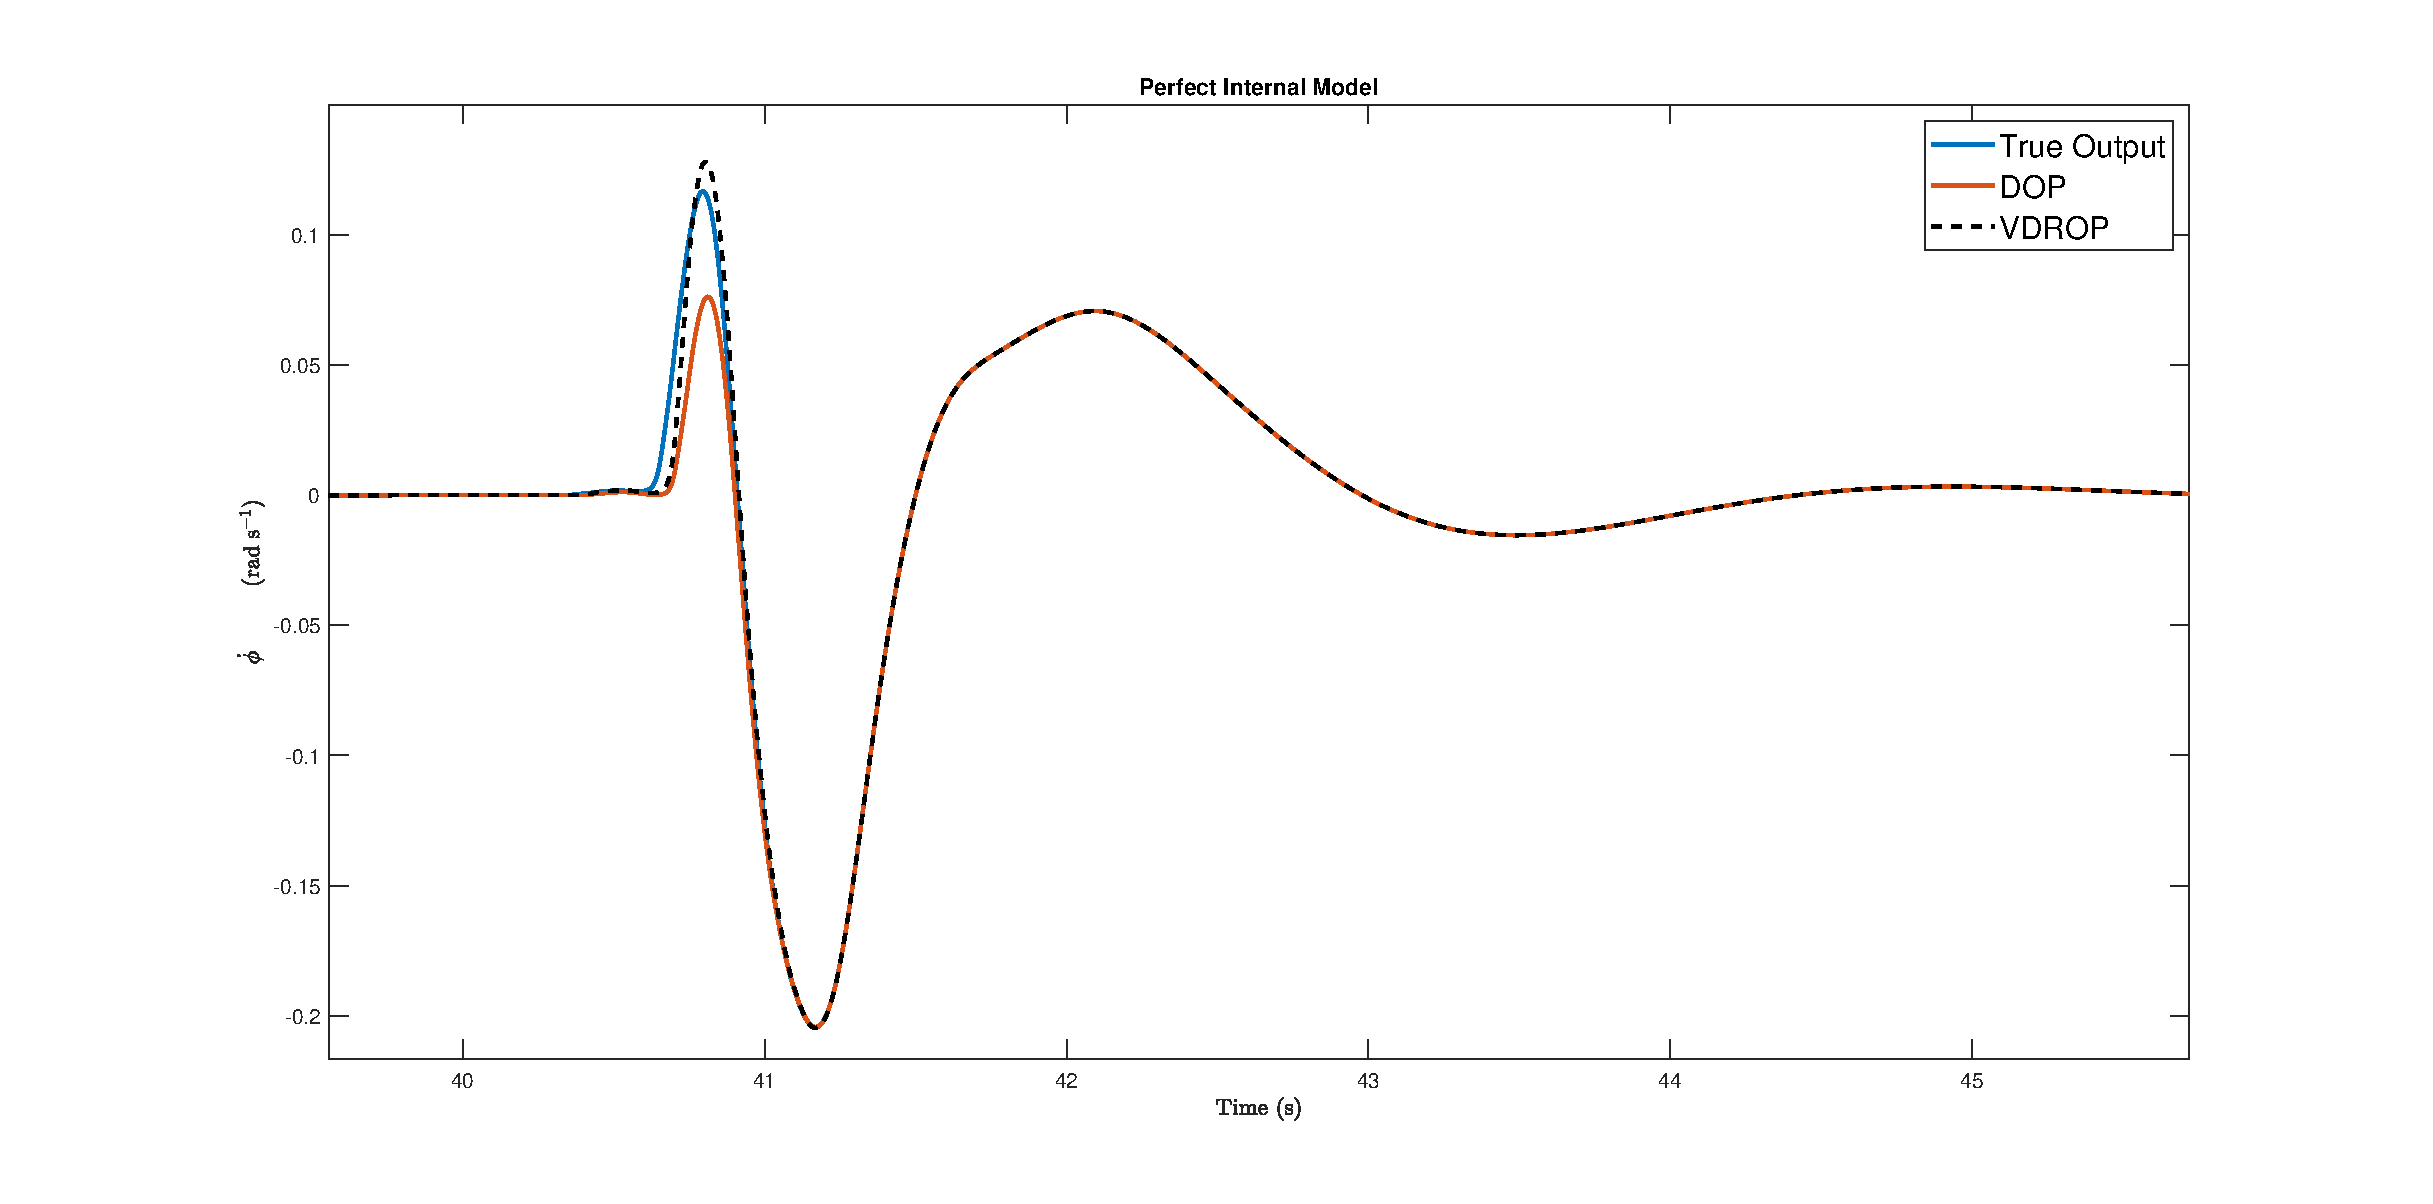
\includegraphics[width=0.49\linewidth]{images/predictor_plots/rate_compare.eps} 
        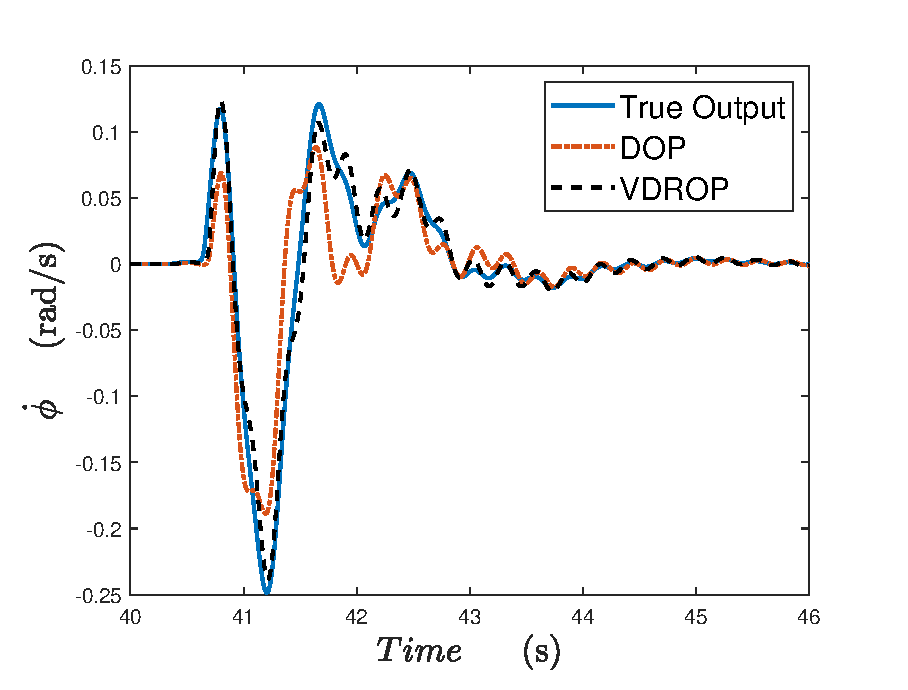
\includegraphics[width=0.49\textwidth]{images/predictor_plots/rate_compare2.eps}}
        \caption{Comparison between true roll rate, and predicted roll rate using the Variant Delay optimal Predictor (VDROP) and the  Discrete Optimal Predictor (DOP).In the left graph a perfect internal model is used while in the right graph imperfections are introduced.}
        \label{fig:predictor_compare}
    \end{subfigure}
    \begin{subfigure}[b]{\textwidth}
        \centering
        \makebox[\textwidth][c]{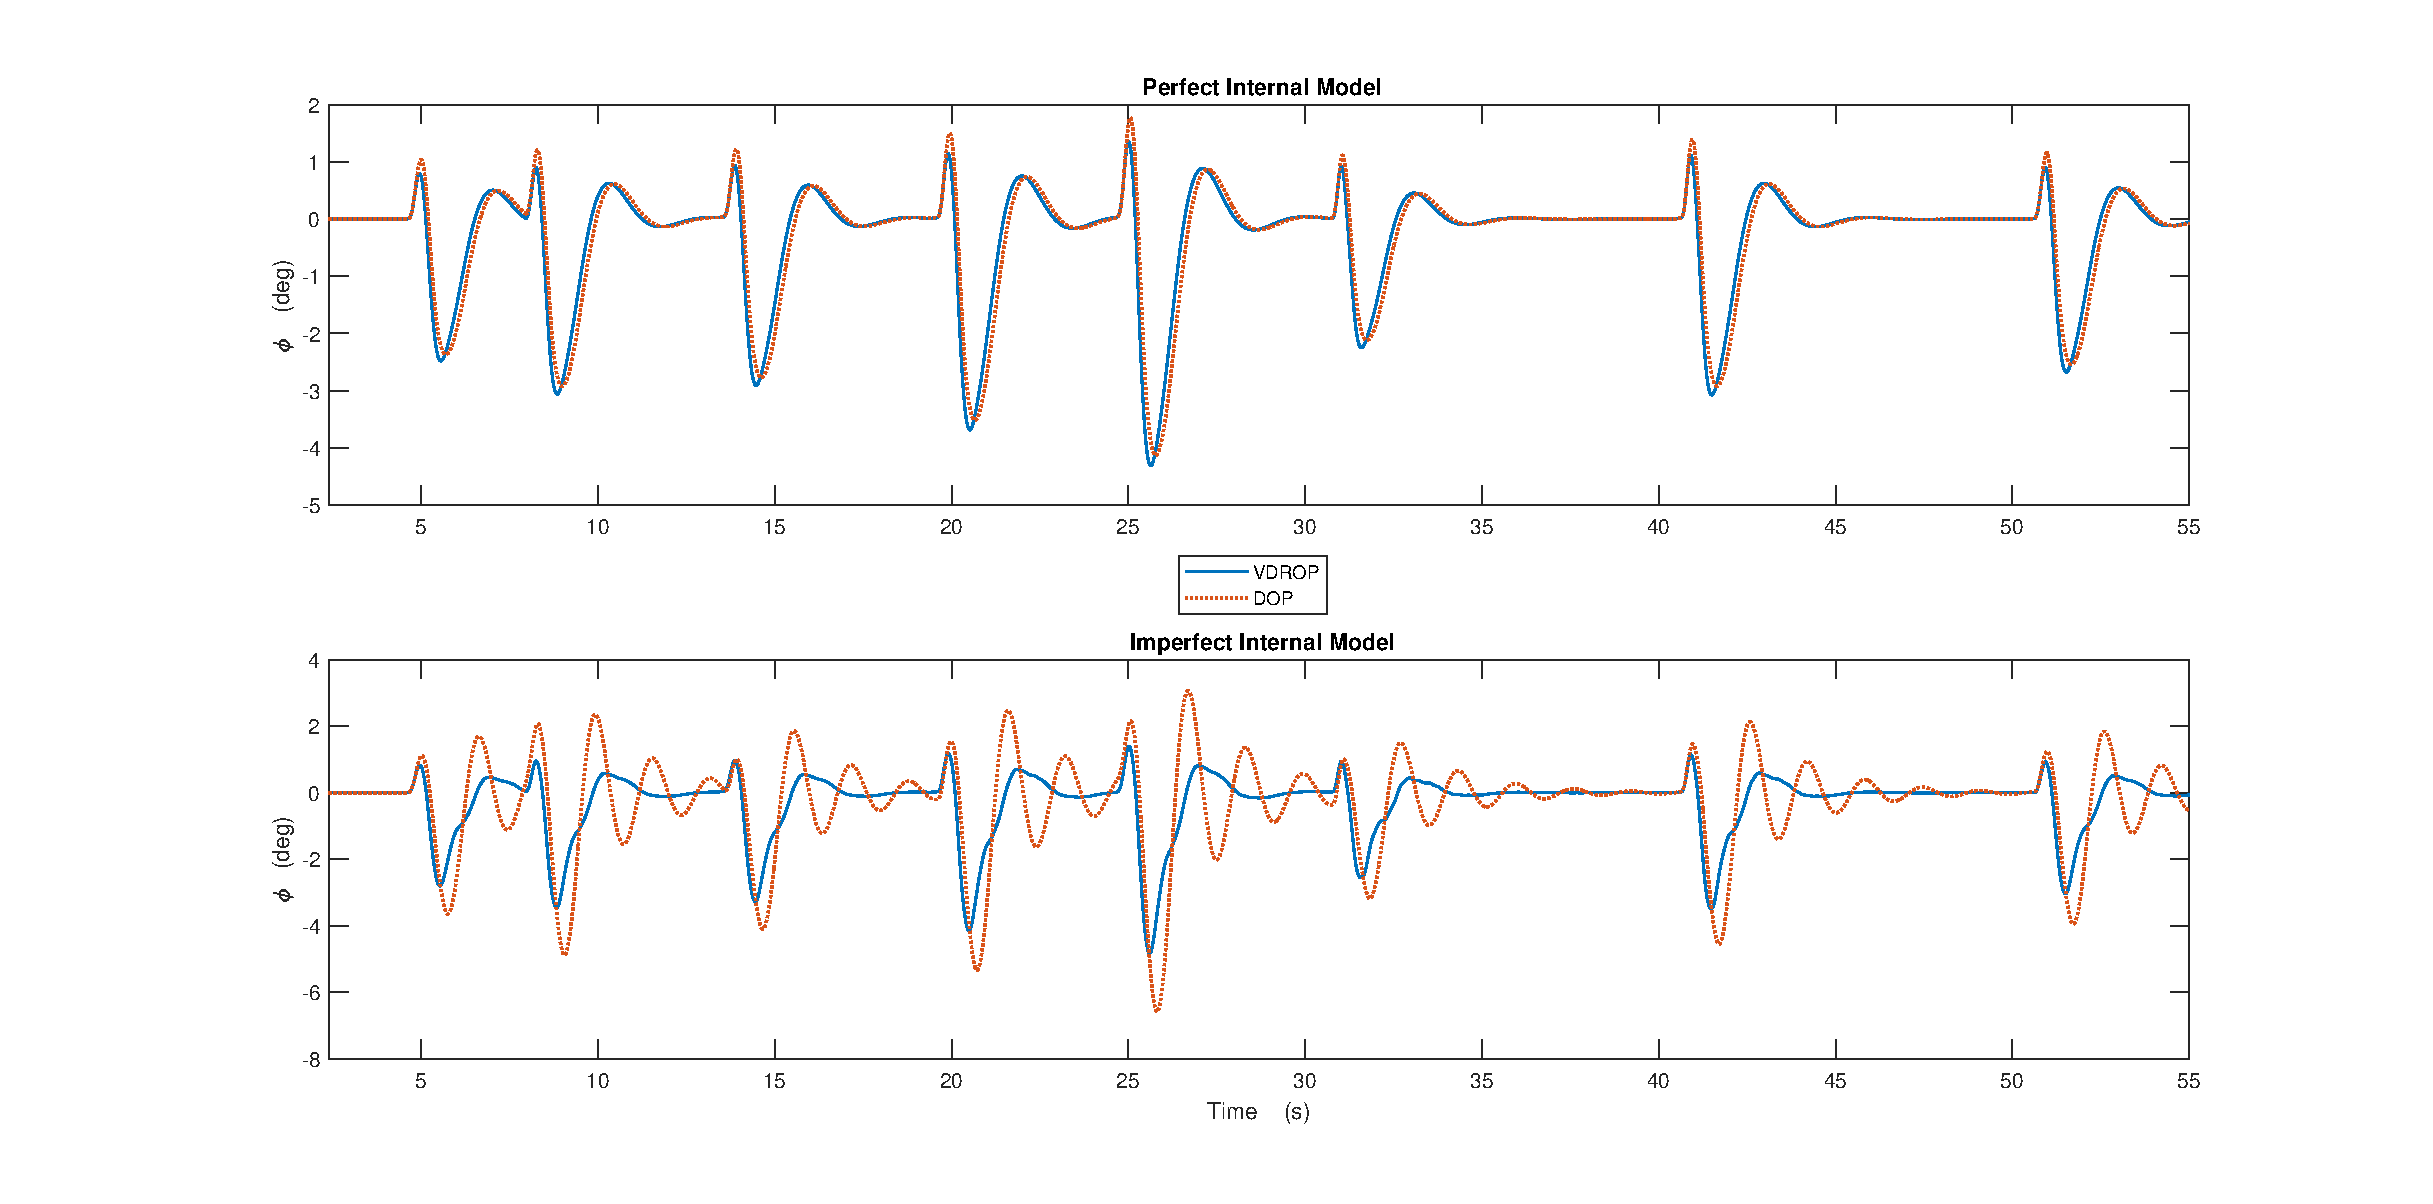
\includegraphics[width=1.3\linewidth]{images/predictor_plots/compare_imperfect.eps}}
        \caption{Roll angle \ensuremath{\phi} compared between  the Variant Delay optimal Predictor and the Discrete Optimal Predictor . In the top graph a perfect internal model is used while in the bottom graph imperfections are introduced.}            
        \label{fig:predictor_compare2}
    \end{subfigure}
    \caption{Results of the simulation using imperfect internal model. In (a) the state estimate of the roll rate is compared among prediction algorithms, while in (b) the roll stabilization response to a prolong run subject to  the different prediction strategies is shown.}
    \label{fig:predictor_compareA}
 \end{figure}


     \begin{figure}
        \centering
        \begin{subfigure}[b]{\textwidth}
            \centering
            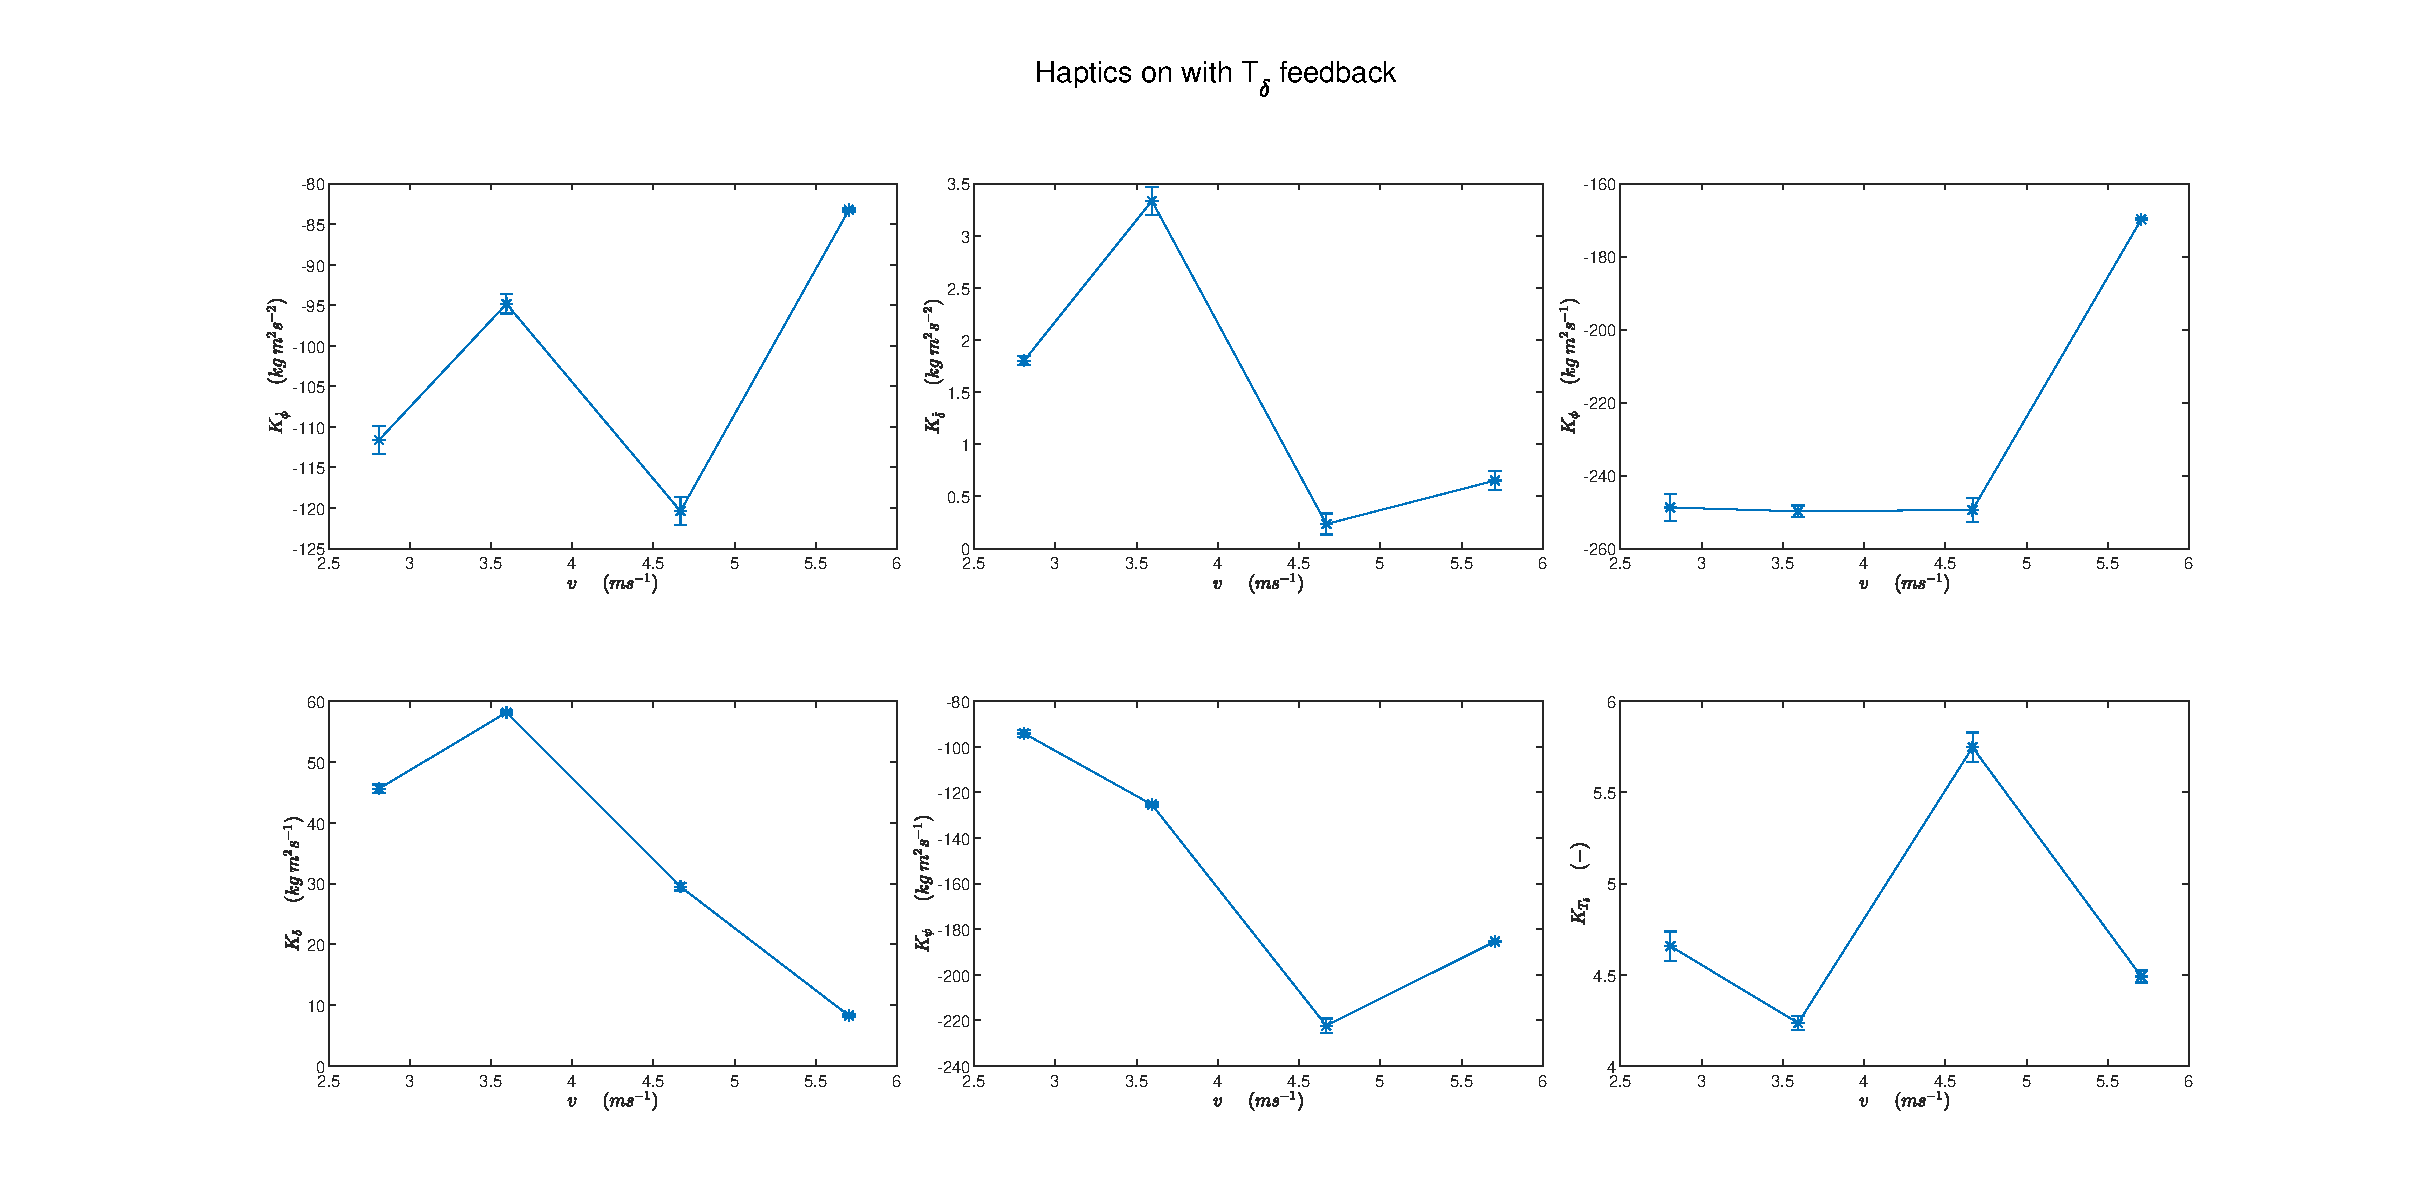
\includegraphics[width=1\linewidth]{images/gain_plots/hap_on_td_predict.eps}
            \caption{}
            \label{fig:gains_speed1}
        \end{subfigure}
        \begin{subfigure}[b]{\textwidth}
            \centering
            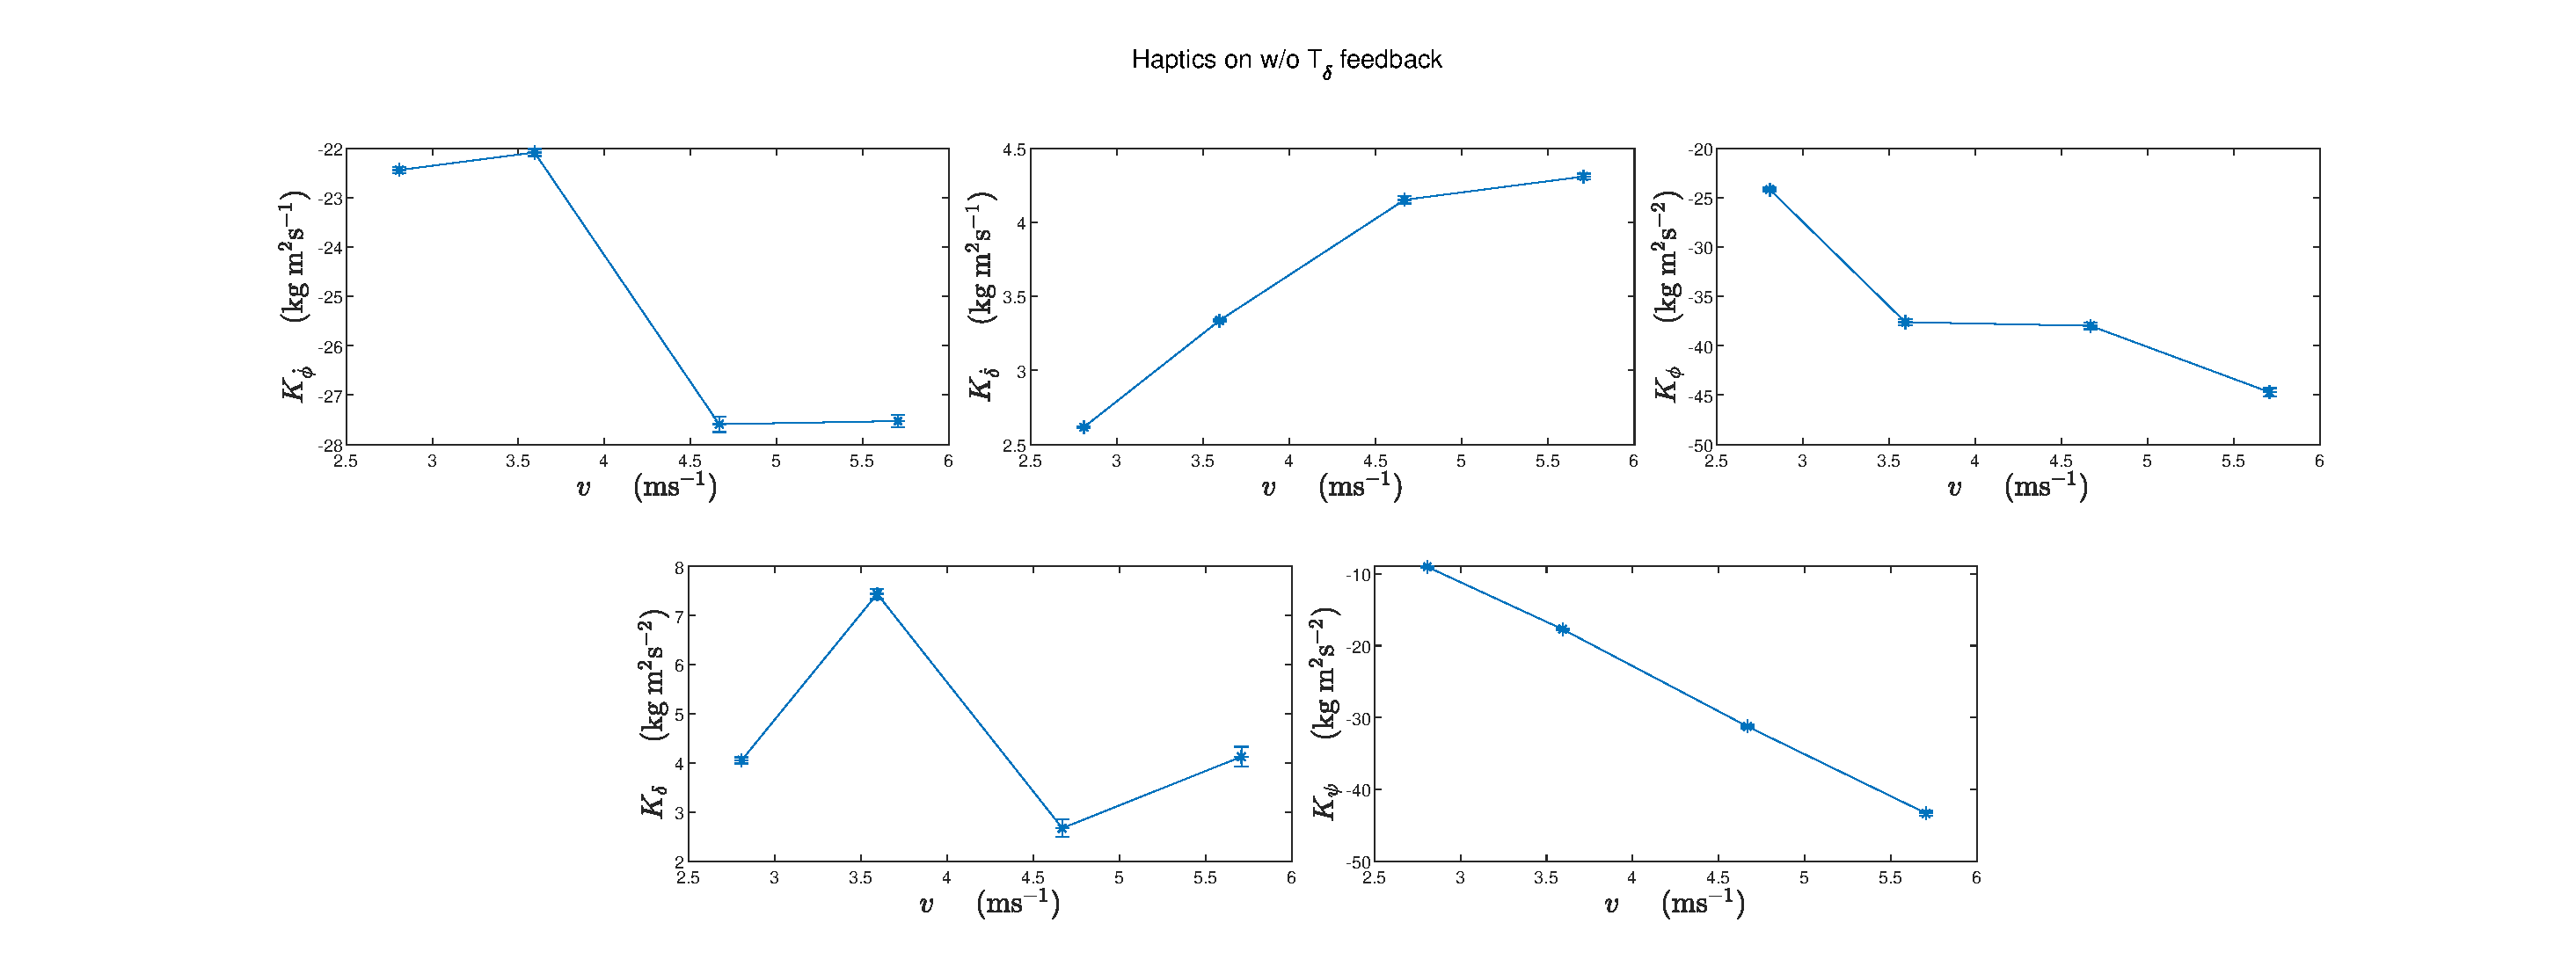
\includegraphics[width=1\linewidth]{images/gain_plots/hap_on_predict.eps}
            \caption{}            
            \label{fig:gains_speed2}
        \end{subfigure}
        \begin{subfigure}[b]{\textwidth}
            \centering
            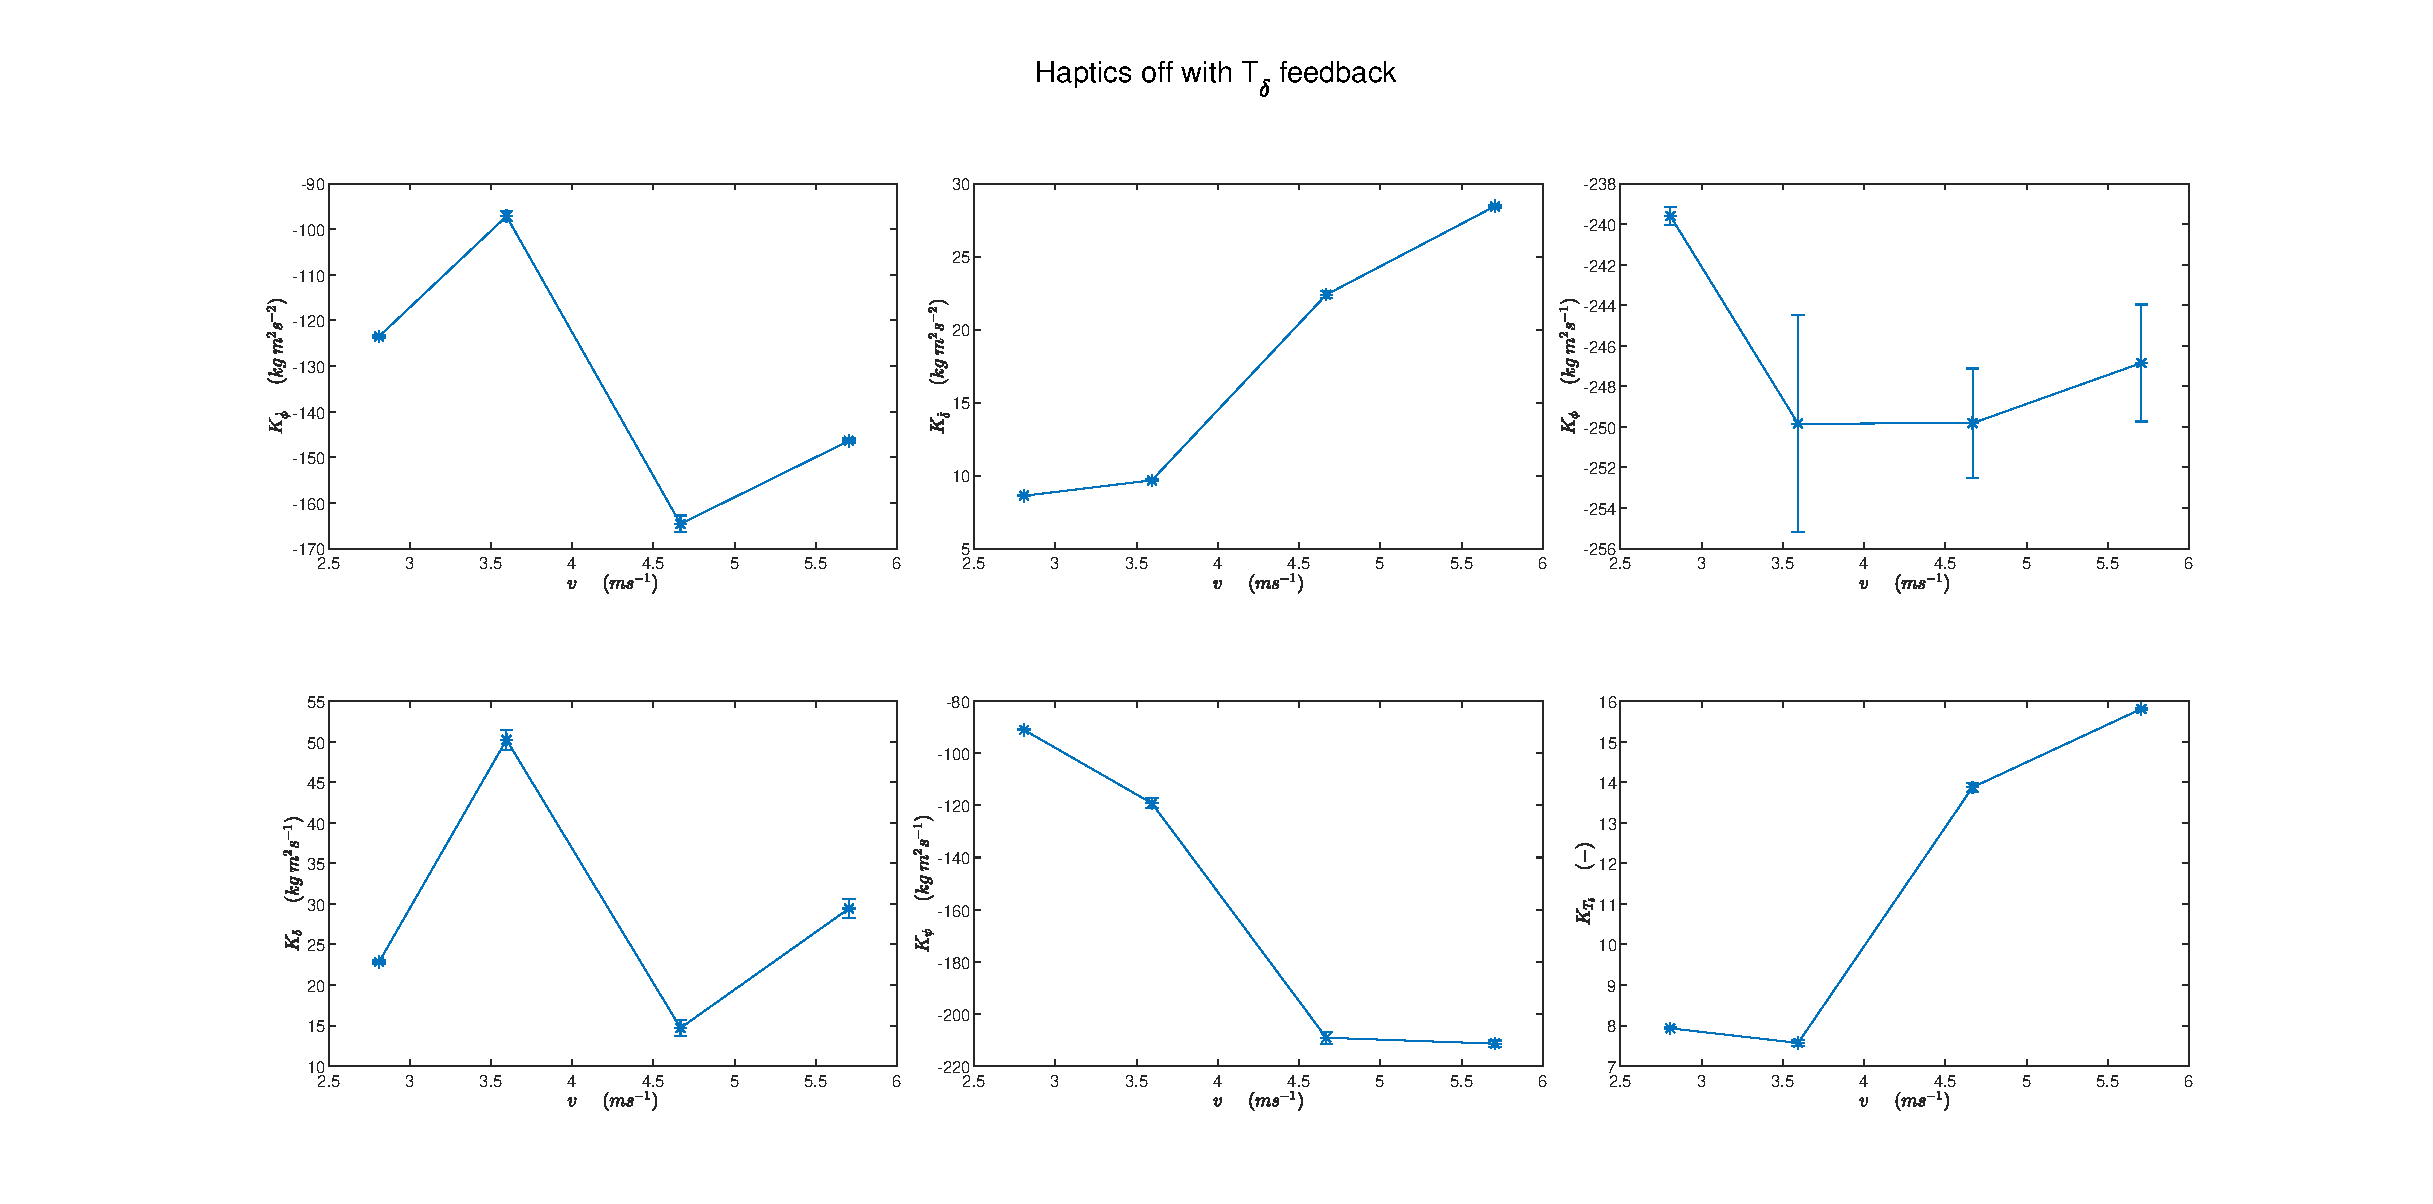
\includegraphics[width=1\linewidth]{images/gain_plots/hap_off_td_predict.eps}
            \caption{}            
            \label{fig:gains_speed3}
        \end{subfigure}
        \caption{Feedback control gains (\ensuremath{K}) as a function of forward velocity (\ensuremath{v}) for the different torque feedback levels for the median rider in the VDROP Model. Error bars indicate the standard errror of the mean calculated from the covariance matrix calculated by \cref{fig:cov_mat}.}
        \label{fig:gains_speed}
     \end{figure}




\begin{table}[]
    \caption{ Results for the zero delay model as estimated for the median rider for all speed levels. Results are presented for the three conditions. Haptic on/off differentiates based on the dynamics of the bicycle model, while "with or w/o \ensuremath{T_\delta} feedback" differentiates based on the structure of the rider control model. The values of the gains are presented as well as their corresponding uncertainty level measured by the coefficient of variation \ensuremath{CV_i}. Additionally, the variance accounted for of the orientation outputs between parametric and non parametric signals is also presented. The derivative gains (\ensuremath{K_{\dot{\phi}}},\ensuremath{K_{\dot{\delta}}}) are measured in \si{\kilogram\square\meter\per\square\second} while the proportional gains (\ensuremath{K_{\phi}},\ensuremath{K_{\delta}},\ensuremath{K_{\psi}}) are measured in \si{\kilogram\square\meter\per\second}. The torque feedback gain \ensuremath{K_{T_\delta}} is dimensionless.}
    \label{tb:no_delay}
    \begin{tabular}{llcccccc}
    \hline
                                                   & Bicycle $\rightarrow$                                              & \multicolumn{4}{c}{Haptic On}                                                                                                                                                                         & \multicolumn{2}{c}{Haptic Off}                                                                    \\ \cline{2-8} 
                                                   & {\color[HTML]{333333} Rider $\;\;\;\;\rightarrow$} & \multicolumn{2}{l}{with $T_\delta$ feedback}                                                      & \multicolumn{2}{l}{w/o  $T_\delta$ feedback}                                                      & \multicolumn{2}{l}{with $T_\delta$ feedback}                                                      \\ \cline{2-8} 
                                                   &                                                                    & \multicolumn{1}{l}{}                        & \multicolumn{1}{l}{}                                & \multicolumn{1}{l}{}                        & \multicolumn{1}{l}{}                                & \multicolumn{1}{l}{}                        & \multicolumn{1}{l}{}                                \\
    \multirow{-2}{*}{Forward Speed}                &                                                                    & \multicolumn{1}{l}{\multirow{-2}{*}{Value}} & \multicolumn{1}{l}{\multirow{-2}{*}{CV ($10^{-4}$)}} & \multicolumn{1}{l}{\multirow{-2}{*}{Value}} & \multicolumn{1}{l}{\multirow{-2}{*}{CV ($10^{-4}$)}} & \multicolumn{1}{l}{\multirow{-2}{*}{Value}} & \multicolumn{1}{l}{\multirow{-2}{*}{CV ($10^{-4}$)}} \\ \hline
                                                   & $K_{\dot{\phi}} $                                                  & -77.17                                      & 114.86                                              & -22.46                                      & 29.77                                               & -115.36                                     & 213.52                                              \\
    \multirow{-2}{*}{2.8 $\si{\meter\per\second}$} & $K_{\dot{\delta}}$                                                 & 2.26                                        & 73.57                                               & 2.58                                        & 18.93                                               & 8.76                                        & 187.30                                              \\
                                                   & $K_{\phi} $                                                        & -164.88                                     & 132.25                                              & -24.50                                      & 73.14                                               & -248.24                                     & 217.05                                              \\
                                                   & $K_\delta $                                                        & 32.75                                       & 150.14                                              & 3.76                                        & 140.96                                              & 29.67                                       & 215.07                                              \\
                                                   & $K_\psi $                                                          & -63.22                                      & 133.29                                              & -9.85                                       & 53.71                                               & -93.44                                      & 223.02                                              \\
                                                   & $K_{T_\delta}$                                                     & 3.51                                        & 176.20                                              & -                                           & -                                                   & 7.53                                        & 223.83                                              \\ \cline{2-8} 
                                                   & $\mathbf{VAF}_\phi$                                                & \multicolumn{2}{c}{77.80}                                                                         & \multicolumn{2}{c}{82.79}                                                                         & \multicolumn{2}{c}{78.37}                                                                         \\
                                                   & $\mathbf{VAF}_\delta$                                              & \multicolumn{2}{c}{98.34}                                                                         & \multicolumn{2}{c}{79.19}                                                                         & \multicolumn{2}{c}{98.20}                                                                         \\
                                                   & $\mathbf{VAF}_\psi$                                                & \multicolumn{2}{c}{93.46}                                                                         & \multicolumn{2}{c}{93.51}                                                                         & \multicolumn{2}{c}{93.74}                                                                         \\
                                                   &                                                                    & \multicolumn{1}{l}{}                        & \multicolumn{1}{l}{}                                & \multicolumn{1}{l}{}                        & \multicolumn{1}{l}{}                                & \multicolumn{1}{l}{}                        & \multicolumn{1}{l}{}                                \\ \hline
                                                   & $K_{\dot{\phi}} $                                                  & -109.94                                     & 146.98                                              & -21.30                                      & 35.99                                               & -78.28                                      & 61.00                                               \\
    \multirow{-2}{*}{3.6 $\si{\meter\per\second}$} & $K_{\dot{\delta}}$                                                 & 8.22                                        & 139.00                                              & 3.30                                        & 24.78                                               & 9.09                                        & 51.11                                               \\
                                                   & $K_{\phi} $                                                        & -248.47                                     & 147.39                                              & -34.64                                      & 71.54                                               & -229.14                                     & 84.40                                               \\
                                                   & $K_\delta $                                                        & 50.78                                       & 147.72                                              & 6.48                                        & 130.57                                              & 53.16                                       & 92.96                                               \\
                                                   & $K_\psi $                                                          & -132.13                                     & 152.08                                              & -17.74                                      & 61.92                                               & -103.75                                     & 74.49                                               \\
                                                   & $K_{T_\delta}$                                                     & 4.52                                        & 167.24                                              & -                                           & -                                                   & 6.89                                        & 64.17                                               \\ \cline{2-8} 
                                                   & $\mathbf{VAF}_\phi$                                                & \multicolumn{2}{c}{79.92}                                                                         & \multicolumn{2}{c}{85.93}                                                                         & \multicolumn{2}{c}{80.89}                                                                         \\
                                                   & $\mathbf{VAF}_\delta$                                              & \multicolumn{2}{c}{98.83}                                                                         & \multicolumn{2}{c}{86.40}                                                                         & \multicolumn{2}{c}{97.08}                                                                         \\
                                                   & $\mathbf{VAF}_\psi$                                                & \multicolumn{2}{c}{95.33}                                                                         & \multicolumn{2}{c}{97.95}                                                                         & \multicolumn{2}{c}{95.15}                                                                         \\
                                                   &                                                                    & \multicolumn{1}{l}{}                        & \multicolumn{1}{l}{}                                & \multicolumn{1}{l}{}                        & \multicolumn{1}{l}{}                                & \multicolumn{1}{l}{}                        & \multicolumn{1}{l}{}                                \\ \hline
                                                   & $K_{\dot{\phi}} $                                                  & -92.50                                      & 117.34                                              & -27.29                                      & 46.40                                               & -102.63                                     & 40.87                                               \\
    \multirow{-2}{*}{4.7 $\si{\meter\per\second}$} & $K_{\dot{\delta}}$                                                 & 4.81                                        & 183.05                                              & 4.25                                        & 41.56                                               & 11.24                                       & 28.38                                               \\
                                                   & $K_{\phi} $                                                        & -183.03                                     & 135.64                                              & -38.17                                      & 76.43                                               & -249.74                                     & 74.10                                               \\
                                                   & $K_\delta $                                                        & 22.57                                       & 237.51                                              & 2.65                                        & 591.87                                              & 63.36                                       & 88.33                                               \\
                                                   & $K_\psi $                                                          & -165.42                                     & 126.89                                              & -33.78                                      & 63.74                                               & -188.67                                     & 58.81                                               \\
                                                   & $K_{T_\delta}$                                                     & 3.42                                        & 174.23                                              & -                                           & -                                                   & 8.98                                        & 13.88                                               \\ \cline{2-8} 
                                                   & $\mathbf{VAF}_\phi$                                                & \multicolumn{2}{c}{77.03}                                                                         & \multicolumn{2}{c}{83.06}                                                                         & \multicolumn{2}{c}{78.60}                                                                         \\
                                                   & $\mathbf{VAF}_\delta$                                              & \multicolumn{2}{c}{97.57}                                                                         & \multicolumn{2}{c}{80.27}                                                                         & \multicolumn{2}{c}{95.57}                                                                         \\
                                                   & $\mathbf{VAF}_\psi$                                                & \multicolumn{2}{c}{91.41}                                                                         & \multicolumn{2}{c}{97.03}                                                                         & \multicolumn{2}{c}{92.48}                                                                         \\
                                                   &                                                                    & \multicolumn{1}{l}{}                        & \multicolumn{1}{l}{}                                & \multicolumn{1}{l}{}                        & \multicolumn{1}{l}{}                                & \multicolumn{1}{l}{}                        & \multicolumn{1}{l}{}                                \\ \hline
                                                   & $K_{\dot{\phi}} $                                                  & -83.90                                      & 117.61                                              & -31.12                                      & 43.99                                               & -76.30                                      & 47.12                                               \\
    \multirow{-2}{*}{5.7 $\si{\meter\per\second}$} & $K_{\dot{\delta}}$                                                 & 5.83                                        & 142.87                                              & 5.58                                        & 40.62                                               & 10.91                                       & 30.23                                               \\
                                                   & $K_{\phi} $                                                        & -166.08                                     & 127.89                                              & -43.64                                      & 67.14                                               & -208.33                                     & 83.09                                               \\
                                                   & $K_\delta $                                                        & 14.85                                       & 98.10                                               & 1.14                                        & 1836.39                                             & 79.44                                       & 75.47                                               \\
                                                   & $K_\psi $                                                          & -186.77                                     & 128.56                                              & -49.82                                      & 52.31                                               & -176.96                                     & 69.82                                               \\
                                                   & $K_{T_\delta}$                                                     & 3.24                                        & 185.07                                              & -                                           & -                                                   & 8.45                                        & 29.67                                               \\ \cline{2-8} 
                                                   & $\mathbf{VAF}_\phi$                                                & \multicolumn{2}{c}{79.17}                                                                         & \multicolumn{2}{c}{84.03}                                                                         & \multicolumn{2}{c}{80.30}                                                                         \\
                                                   & $\mathbf{VAF}_\delta$                                              & \multicolumn{2}{c}{97.51}                                                                         & \multicolumn{2}{c}{84.09}                                                                         & \multicolumn{2}{c}{94.71}                                                                         \\
                                                   & $\mathbf{VAF}_\psi$                                                & \multicolumn{2}{c}{90.97}                                                                         & \multicolumn{2}{c}{96.41}                                                                         & \multicolumn{2}{c}{91.56}                                                                        
    \end{tabular}
    \end{table}

\begin{table}[]
    \caption{ Results for the variable delay model as estimated for the median rider for all speed levels. Results are presented for the three conditions. Haptic on/off differentiates based on the dynamics of the bicycle model, while "with or w/o \ensuremath{T_\delta} feedback" differentiates based on the structure of the rider control model. The values of the gains are presented as well as their corresponding uncertainty level measured by the coefficient of variation \ensuremath{CV_i}. Additionally, the variance accounted for of the orientation outputs between parametric and non parametric signals is also presented. The derivative gains (\ensuremath{K_{\dot{\phi}}},\ensuremath{K_{\dot{\delta}}}) are measured in \si{\kilogram\square\meter\per\square\second} while the proportional gains (\ensuremath{K_{\phi}},\ensuremath{K_{\delta}},\ensuremath{K_{\psi}}) are measured in \si{\kilogram\square\meter\per\second}. The torque feedback gain \ensuremath{K_{T_\delta}} is dimensionless.}
    \label{tb:variable}
    \begin{tabular}{llcccccc}
    \hline
                                                   & Bicycle $\rightarrow$                                  & \multicolumn{4}{c}{Haptic On}                                                                                                                                                                           & \multicolumn{2}{c}{Haptic Off}                                                                     \\ \cline{2-8} 
                                                   & {\color[HTML]{333333} Rider $\;\;\;\;\rightarrow$} & \multicolumn{2}{l}{with $T_\delta$ feedback}                                                       & \multicolumn{2}{l}{w/o  $T_\delta$ feedback}                                                       & \multicolumn{2}{l}{with $T_\delta$ feedback}                                                       \\ \cline{2-8} 
                                                   &                                                        & \multicolumn{1}{l}{}                        & \multicolumn{1}{l}{}                                 & \multicolumn{1}{l}{}                        & \multicolumn{1}{l}{}                                 & \multicolumn{1}{l}{}                        & \multicolumn{1}{l}{}                                 \\
    \multirow{-2}{*}{Forward Speed}                &                                                        & \multicolumn{1}{l}{\multirow{-2}{*}{Value}} & \multicolumn{1}{l}{\multirow{-2}{*}{CV ($10^{-4}$)}} & \multicolumn{1}{l}{\multirow{-2}{*}{Value}} & \multicolumn{1}{l}{\multirow{-2}{*}{CV ($10^{-4}$)}} & \multicolumn{1}{l}{\multirow{-2}{*}{Value}} & \multicolumn{1}{l}{\multirow{-2}{*}{CV ($10^{-4}$)}} \\ \hline
                                                   & $K_{\dot{\phi}} $                                      & -68.53                                      & 38.72                                                & -14.93                                      & 37.52                                                & -28.19                                      & 35.15                                                \\
    \multirow{-2}{*}{2.8 $\si{\meter\per\second}$} & $K_{\dot{\delta}}$                                     & 2.09                                        & 110.32                                               & 2.30                                        & 32.17                                                & 2.65                                        & 13.18                                                \\
                                                   & $K_{\phi} $                                            & -146.29                                     & 72.07                                                & -16.98                                      & 92.51                                                & -79.20                                      & 78.41                                                \\
                                                   & $K_\delta $                                            & 22.18                                       & 95.38                                                & 4.62                                        & 103.75                                               & 10.51                                       & 93.36                                                \\
                                                   & $K_\psi $                                              & -40.34                                      & 56.18                                                & -3.78                                       & 116.84                                               & -14.53                                      & 67.08                                                \\
                                                   & $K_{T_\delta}$                                         & 3.52                                        & 64.80                                                & -                                           & -                                                    & 2.59                                        & 29.48                                                \\ \cline{2-8} 
                                                   & $\mathbf{VAF}_\phi$                                    & \multicolumn{2}{c}{81.15}                                                                          & \multicolumn{2}{c}{69.61}                                                                          & \multicolumn{2}{c}{80.01}                                                                          \\
                                                   & $\mathbf{VAF}_\delta$                                  & \multicolumn{2}{c}{93.43}                                                                          & \multicolumn{2}{c}{23.34}                                                                          & \multicolumn{2}{c}{66.84}                                                                          \\
                                                   & $\mathbf{VAF}_\psi$                                    & \multicolumn{2}{c}{93.78}                                                                          & \multicolumn{2}{c}{69.67}                                                                          & \multicolumn{2}{c}{83.30}                                                                          \\
                                                   &                                                        & \multicolumn{1}{l}{}                        & \multicolumn{1}{l}{}                                 & \multicolumn{1}{l}{}                        & \multicolumn{1}{l}{}                                 & \multicolumn{1}{l}{}                        & \multicolumn{1}{l}{}                                 \\ \hline
                                                   & $K_{\dot{\phi}} $                                      & -51.02                                      & 56.62                                                & -15.40                                      & 55.90                                                & -21.25                                      & 51.31                                                \\
    \multirow{-2}{*}{3.6 $\si{\meter\per\second}$} & $K_{\dot{\delta}}$                                     & 2.50                                        & 170.45                                               & 2.81                                        & 50.20                                                & 2.79                                        & 17.72                                                \\
                                                   & $K_{\phi} $                                            & -120.51                                     & 85.28                                                & -22.82                                      & 102.83                                               & -76.41                                      & 90.89                                                \\
                                                   & $K_\delta $                                            & 16.58                                       & 153.27                                               & 3.94                                        & 243.76                                               & 17.14                                       & 84.92                                                \\
                                                   & $K_\psi $                                              & -43.06                                      & 79.41                                                & -7.37                                       & 147.32                                               & -13.30                                      & 103.52                                               \\
                                                   & $K_{T_\delta}$                                         & 3.42                                        & 62.79                                                & -                                           & -                                                    & 3.09                                        & 21.20                                                \\ \cline{2-8} 
                                                   & $\mathbf{VAF}_\phi$                                    & \multicolumn{2}{c}{82.85}                                                                          & \multicolumn{2}{c}{79.48}                                                                          & \multicolumn{2}{c}{73.14}                                                                          \\
                                                   & $\mathbf{VAF}_\delta$                                  & \multicolumn{2}{c}{91.63}                                                                          & \multicolumn{2}{c}{53.29}                                                                          & \multicolumn{2}{c}{52.83}                                                                          \\
                                                   & $\mathbf{VAF}_\psi$                                    & \multicolumn{2}{c}{95.10}                                                                          & \multicolumn{2}{c}{84.88}                                                                          & \multicolumn{2}{c}{71.58}                                                                          \\
                                                   &                                                        & \multicolumn{1}{l}{}                        & \multicolumn{1}{l}{}                                 & \multicolumn{1}{l}{}                        & \multicolumn{1}{l}{}                                 & \multicolumn{1}{l}{}                        & \multicolumn{1}{l}{}                                 \\ \hline
                                                   & $K_{\dot{\phi}} $                                      & -51.78                                      & 64.60                                                & -19.26                                      & 349.70                                               & -14.88                                      & 55.92                                                \\
    \multirow{-2}{*}{4.7 $\si{\meter\per\second}$} & $K_{\dot{\delta}}$                                     & 2.75                                        & 160.68                                               & 4.42                                        & 438.96                                               & 3.04                                        & 20.62                                                \\
                                                   & $K_{\phi} $                                            & -136.22                                     & 105.15                                               & -27.02                                      & 111.78                                               & -48.91                                      & 115.90                                               \\
                                                   & $K_\delta $                                            & 3.21                                        & 1156.00                                              & 0.01                                        & 492609.67                                            & 16.01                                       & 99.26                                                \\
                                                   & $K_\psi $                                              & -64.43                                      & 87.60                                                & -14.29                                      & 412.99                                               & -10.82                                      & 119.48                                               \\
                                                   & $K_{T_\delta}$                                         & 3.70                                        & 63.91                                                & -                                           & -                                                    & 2.61                                        & 30.62                                                \\ \cline{2-8} 
                                                   & $\mathbf{VAF}_\phi$                                    & \multicolumn{2}{c}{77.86}                                                                          & \multicolumn{2}{c}{71.14}                                                                          & \multicolumn{2}{c}{63.73}                                                                          \\
                                                   & $\mathbf{VAF}_\delta$                                  & \multicolumn{2}{c}{81.63}                                                                          & \multicolumn{2}{c}{36.19}                                                                          & \multicolumn{2}{c}{15.61}                                                                          \\
                                                   & $\mathbf{VAF}_\psi$                                    & \multicolumn{2}{c}{90.32}                                                                          & \multicolumn{2}{c}{80.57}                                                                          & \multicolumn{2}{c}{55.71}                                                                          \\
                                                   &                                                        & \multicolumn{1}{l}{}                        & \multicolumn{1}{l}{}                                 & \multicolumn{1}{l}{}                        & \multicolumn{1}{l}{}                                 & \multicolumn{1}{l}{}                        & \multicolumn{1}{l}{}                                 \\ \hline
                                                   & $K_{\dot{\phi}} $                                      & -38.58                                      & 136.91                                               & -19.65                                      & 110.85                                               & -10.10                                      & 62.29                                                \\
    \multirow{-2}{*}{5.7 $\si{\meter\per\second}$} & $K_{\dot{\delta}}$                                     & 1.13                                        & 2085.75                                              & 5.42                                        & 128.32                                               & 3.08                                        & 21.38                                                \\
                                                   & $K_{\phi} $                                            & -120.59                                     & 120.57                                               & -33.34                                      & 117.63                                               & -30.95                                      & 133.76                                               \\
                                                   & $K_\delta $                                            & 0.00                                        & 3969013.40                                           & 0.01                                        & 280859.33                                            & 18.46                                       & 79.69                                                \\
                                                   & $K_\psi $                                              & -60.65                                      & 95.03                                                & -19.20                                      & 183.00                                               & -8.17                                       & 131.56                                               \\
                                                   & $K_{T_\delta}$                                         & 4.27                                        & 191.50                                               & -                                           & -                                                    & 2.58                                        & 26.58                                                \\ \cline{2-8} 
                                                   & $\mathbf{VAF}_\phi$                                    & \multicolumn{2}{c}{73.65}                                                                          & \multicolumn{2}{c}{70.08}                                                                          & \multicolumn{2}{c}{49.58}                                                                          \\
                                                   & $\mathbf{VAF}_\delta$                                  & \multicolumn{2}{c}{77.99}                                                                          & \multicolumn{2}{c}{40.64}                                                                          & \multicolumn{2}{c}{-}                                                                              \\
                                                   & $\mathbf{VAF}_\psi$                                    & \multicolumn{2}{c}{84.32}                                                                          & \multicolumn{2}{c}{79.50}                                                                          & \multicolumn{2}{c}{39.90}                                                                         
    \end{tabular}
    \end{table}
% Please add the following required packages to your document preamble:
% \usepackage{multirow}
% \usepackage[table,xcdraw]{xcolor}
% If you use beamer only pass "xcolor=table" option, i.e. \documentclass[xcolor=table]{beamer}
\begin{table}[]
    \caption{ Results for the VDROP model as estimated for the median rider for all speed levels. Results are presented for the three conditions. Haptic on/off differentiates based on the dynamics of the bicycle model, while "with or w/o \ensuremath{T_\delta} feedback" differentiates based on the structure of the rider control model. The values of the gains are presented as well as their corresponding uncertainty level measured by the coefficient of variation \ensuremath{CV_i}. Additionally, the variance accounted for of the orientation outputs between parametric and non parametric signals is also presented. The derivative gains (\ensuremath{K_{\dot{\phi}}},\ensuremath{K_{\dot{\delta}}}) are measured in \si{\kilogram\square\meter\per\square\second} while the proportional gains (\ensuremath{K_{\phi}},\ensuremath{K_{\delta}},\ensuremath{K_{\psi}}) are measured in \si{\kilogram\square\meter\per\second}. The torque feedback gain \ensuremath{K_{T_\delta}} is dimensionless.}
    \label{tb:predict}
    \begin{tabular}{llcccccc}
    \hline
                                                   & Bicycle $\rightarrow$                                  & \multicolumn{4}{c}{Haptics On}                                                                                                                                                                          & \multicolumn{2}{c}{Haptics Off}                                                                    \\ \cline{2-8} 
                                                   & {\color[HTML]{333333} Rider $\;\;\;\;\;\;\rightarrow$} & \multicolumn{2}{l}{with $T_\delta$ feedback}                                                       & \multicolumn{2}{l}{w/o  $T_\delta$ feedback}                                                       & \multicolumn{2}{l}{with $T_\delta$ feedback}                                                       \\ \cline{2-8} 
                                                   &                                                        & \multicolumn{1}{l}{}                        & \multicolumn{1}{l}{}                                 & \multicolumn{1}{l}{}                        & \multicolumn{1}{l}{}                                 & \multicolumn{1}{l}{}                        & \multicolumn{1}{l}{}                                 \\
    \multirow{-2}{*}{Forward Speed}                &                                                        & \multicolumn{1}{l}{\multirow{-2}{*}{Value}} & \multicolumn{1}{l}{\multirow{-2}{*}{CV ($10^{-4}$)}} & \multicolumn{1}{l}{\multirow{-2}{*}{Value}} & \multicolumn{1}{l}{\multirow{-2}{*}{CV ($10^{-4}$)}} & \multicolumn{1}{l}{\multirow{-2}{*}{Value}} & \multicolumn{1}{l}{\multirow{-2}{*}{CV ($10^{-4}$)}} \\ \hline
                                                   & $K_{\dot{\phi}} $                                      & -111.62                                     & 152.10                                               & -22.44                                      & 28.45                                                & -123.53                                     & 27.90                                                \\
    \multirow{-2}{*}{2.8 $\si{\meter\per\second}$} & $K_{\dot{\delta}}$                                     & 1.80                                        & 234.11                                               & 2.62                                        & 14.59                                                & 8.62                                        & 35.62                                                \\
                                                   & $K_{\phi} $                                            & -248.74                                     & 151.15                                               & -24.17                                      & 84.44                                                & -239.60                                     & 18.65                                                \\
                                                   & $K_\delta $                                            & 45.60                                       & 150.24                                               & 4.05                                        & 147.97                                               & 22.82                                       & 90.52                                                \\
                                                   & $K_\psi $                                              & -94.18                                      & 156.50                                               & -9.03                                       & 65.63                                                & -91.07                                      & 14.16                                                \\
                                                   & $K_{T_\delta}$                                         & 4.66                                        & 170.99                                               & -                                           & -                                                    & 7.93                                        & 27.78                                                \\ \cline{2-8} 
                                                   & $\mathbf{VAF}_\phi$                                    & \multicolumn{2}{c}{78.80}                                                                          & \multicolumn{2}{c}{82.33}                                                                          & \multicolumn{2}{c}{80.67}                                                                          \\
                                                   & $\mathbf{VAF}_\delta$                                  & \multicolumn{2}{c}{98.21}                                                                          & \multicolumn{2}{c}{68.99}                                                                          & \multicolumn{2}{c}{97.59}                                                                          \\
                                                   & $\mathbf{VAF}_\psi$                                    & \multicolumn{2}{c}{94.04}                                                                          & \multicolumn{2}{c}{90.77}                                                                          & \multicolumn{2}{c}{94.95}                                                                          \\
                                                   &                                                        & \multicolumn{1}{l}{}                        & \multicolumn{1}{l}{}                                 & \multicolumn{1}{l}{}                        & \multicolumn{1}{l}{}                                 & \multicolumn{1}{l}{}                        & \multicolumn{1}{l}{}                                 \\ \hline
                                                   & $K_{\dot{\phi}} $                                      & -94.83                                      & 125.80                                               & -22.08                                      & 33.58                                                & -97.15                                      & 115.92                                               \\
    \multirow{-2}{*}{3.6 $\si{\meter\per\second}$} & $K_{\dot{\delta}}$                                     & 3.33                                        & 404.51                                               & 3.34                                        & 17.01                                                & 9.68                                        & 75.60                                                \\
                                                   & $K_{\phi} $                                            & -249.80                                     & 64.02                                                & -37.61                                      & 80.02                                                & -249.84                                     & 214.29                                               \\
                                                   & $K_\delta $                                            & 58.12                                       & 63.15                                                & 7.44                                        & 140.22                                               & 50.23                                       & 247.35                                               \\
                                                   & $K_\psi $                                              & -125.36                                     & 97.89                                                & -17.72                                      & 66.95                                                & -119.20                                     & 160.68                                               \\
                                                   & $K_{T_\delta}$                                         & 4.24                                        & 91.84                                                & -                                           & -                                                    & 7.57                                        & 95.88                                                \\ \cline{2-8} 
                                                   & $\mathbf{VAF}_\phi$                                    & \multicolumn{2}{c}{81.66}                                                                          & \multicolumn{2}{c}{86.50}                                                                          & \multicolumn{2}{c}{83.35}                                                                          \\
                                                   & $\mathbf{VAF}_\delta$                                  & \multicolumn{2}{c}{97.33}                                                                          & \multicolumn{2}{c}{79.27}                                                                          & \multicolumn{2}{c}{96.15}                                                                          \\
                                                   & $\mathbf{VAF}_\psi$                                    & \multicolumn{2}{c}{96.13}                                                                          & \multicolumn{2}{c}{96.97}                                                                          & \multicolumn{2}{c}{96.80}                                                                          \\
                                                   &                                                        & \multicolumn{1}{l}{}                        & \multicolumn{1}{l}{}                                 & \multicolumn{1}{l}{}                        & \multicolumn{1}{l}{}                                 & \multicolumn{1}{l}{}                        & \multicolumn{1}{l}{}                                 \\ \hline
                                                   & $K_{\dot{\phi}} $                                      & -120.38                                     & 145.55                                               & -27.59                                      & 56.00                                                & -164.59                                     & 112.31                                               \\
    \multirow{-2}{*}{4.7 $\si{\meter\per\second}$} & $K_{\dot{\delta}}$                                     & 0.24                                        & 4252.46                                              & 4.15                                        & 59.72                                                & 22.39                                       & 106.46                                               \\
                                                   & $K_{\phi} $                                            & -249.40                                     & 133.42                                               & -37.98                                      & 90.28                                                & -249.82                                     & 107.93                                               \\
                                                   & $K_\delta $                                            & 29.49                                       & 210.73                                               & 2.67                                        & 665.03                                               & 14.70                                       & 649.60                                               \\
                                                   & $K_\psi $                                              & -222.31                                     & 143.06                                               & -31.24                                      & 81.57                                                & -209.12                                     & 111.47                                               \\
                                                   & $K_{T_\delta}$                                         & 5.75                                        & 141.98                                               & -                                           & -                                                    & 13.87                                       & 78.12                                                \\ \cline{2-8} 
                                                   & $\mathbf{VAF}_\phi$                                    & \multicolumn{2}{c}{79.21}                                                                          & \multicolumn{2}{c}{81.88}                                                                          & \multicolumn{2}{c}{80.97}                                                                          \\
                                                   & $\mathbf{VAF}_\delta$                                  & \multicolumn{2}{c}{97.07}                                                                          & \multicolumn{2}{c}{70.43}                                                                          & \multicolumn{2}{c}{90.44}                                                                          \\
                                                   & $\mathbf{VAF}_\psi$                                    & \multicolumn{2}{c}{92.97}                                                                          & \multicolumn{2}{c}{95.43}                                                                          & \multicolumn{2}{c}{95.93}                                                                          \\
                                                   &                                                        & \multicolumn{1}{l}{}                        & \multicolumn{1}{l}{}                                 & \multicolumn{1}{l}{}                        & \multicolumn{1}{l}{}                                 & \multicolumn{1}{l}{}                        & \multicolumn{1}{l}{}                                 \\ \hline
                                                   & $K_{\dot{\phi}} $                                      & -83.24                                      & 24.27                                                & -27.53                                      & 46.08                                                & -146.38                                     & 35.81                                                \\
    \multirow{-2}{*}{5.7 $\si{\meter\per\second}$} & $K_{\dot{\delta}}$                                     & 0.65                                        & 1394.64                                              & 4.31                                        & 43.06                                                & 28.45                                       & 31.76                                                \\
                                                   & $K_{\phi} $                                            & -169.81                                     & 13.03                                                & -44.71                                      & 92.82                                                & -246.85                                     & 116.80                                               \\
                                                   & $K_\delta $                                            & 8.29                                        & 278.33                                               & 4.13                                        & 493.77                                               & 29.42                                       & 401.88                                               \\
                                                   & $K_\psi $                                              & -185.36                                     & 6.72                                                 & -43.34                                      & 72.02                                                & -211.40                                     & 56.88                                                \\
                                                   & $K_{T_\delta}$                                         & 4.49                                        & 72.85                                                & -                                           & -                                                    & 15.81                                       & 10.28                                                \\ \cline{2-8} 
                                                   & $\mathbf{VAF}_\phi$                                    & \multicolumn{2}{c}{82.35}                                                                          & \multicolumn{2}{c}{85.06}                                                                          & \multicolumn{2}{c}{80.57}                                                                          \\
                                                   & $\mathbf{VAF}_\delta$                                  & \multicolumn{2}{c}{96.12}                                                                          & \multicolumn{2}{c}{75.40}                                                                          & \multicolumn{2}{c}{87.27}                                                                          \\
                                                   & $\mathbf{VAF}_\psi$                                    & \multicolumn{2}{c}{93.83}                                                                          & \multicolumn{2}{c}{97.03}                                                                          & \multicolumn{2}{c}{93.59}                                                                         
    \end{tabular}
    \end{table}
% \begin{table}[]
%     \caption{ Results for the ROP model as estimated for the median rider for all speed levels. Results are presented for the three conditions. Haptic on/off differentiates based on the dynamics of the bicycle model, while "with or w/o \ensuremath{T_\delta} feedback" differentiates based on the structure of the rider control model. The values of the gains are presented as well as their corresponding uncertainty level measured by the coefficient of variation \ensuremath{CV_i}. Additionally, the variance accounted for of the orientation outputs between parametric and non parametric signals is also presented. The derivative gains (\ensuremath{K_{\dot{\phi}}},\ensuremath{K_{\dot{\delta}}}) are measured in \si{\kilogram\square\meter\per\square\second} while the proportional gains (\ensuremath{K_{\phi}},\ensuremath{K_{\delta}},\ensuremath{K_{\psi}}) are measured in \si{\kilogram\square\meter\per\second}. The torque feedback gain \ensuremath{K_{T_\delta}} is dimensionless.}
%     \label{tb:predict}
%     \begin{tabular}{llcccccc}
%     \hline
%                                                    & Bicycle $\rightarrow$                                  & \multicolumn{4}{c}{Haptics On}                                                                                                                                                                          & \multicolumn{2}{c}{Haptics Off}                                                                    \\ \cline{2-8} 
%                                                    & {\color[HTML]{333333} Rider $\;\;\;\;\rightarrow$} & \multicolumn{2}{l}{with $T_\delta$ feedback}                                                       & \multicolumn{2}{l}{w/o  $T_\delta$ feedback}                                                       & \multicolumn{2}{l}{with $T_\delta$ feedback}                                                       \\ \cline{2-8} 
%                                                    &                                                        & \multicolumn{1}{l}{}                        & \multicolumn{1}{l}{}                                 & \multicolumn{1}{l}{}                        & \multicolumn{1}{l}{}                                 & \multicolumn{1}{l}{}                        & \multicolumn{1}{l}{}                                 \\
%     \multirow{-2}{*}{Forward Speed}                &                                                        & \multicolumn{1}{l}{\multirow{-2}{*}{Value}} & \multicolumn{1}{l}{\multirow{-2}{*}{CV ($10^{-4}$)}} & \multicolumn{1}{l}{\multirow{-2}{*}{Value}} & \multicolumn{1}{l}{\multirow{-2}{*}{CV ($10^{-4}$)}} & \multicolumn{1}{l}{\multirow{-2}{*}{Value}} & \multicolumn{1}{l}{\multirow{-2}{*}{CV ($10^{-4}$)}} \\ \hline
%                                                    & $K_{\dot{\phi}} $                                      & -117.07                                     & 153.96                                               & -21.11                                      & 30.98                                                & -137.02                                     & 116.70                                               \\
%     \multirow{-2}{*}{2.8 $\si{\meter\per\second}$} & $K_{\dot{\delta}}$                                     & 3.52                                        & 150.97                                               & 2.59                                        & 18.53                                                & 10.91                                       & 108.44                                               \\
%                                                    & $K_{\phi} $                                            & -248.50                                     & 159.45                                               & -24.00                                      & 81.61                                                & -249.38                                     & 118.66                                               \\
%                                                    & $K_\delta $                                            & 47.43                                       & 167.35                                               & 4.39                                        & 131.79                                               & 23.39                                       & 153.29                                               \\
%                                                    & $K_\psi $                                              & -94.42                                      & 161.46                                               & -8.72                                       & 61.07                                                & -97.63                                      & 119.57                                               \\
%                                                    & $K_{T_\delta}$                                         & 5.26                                        & 190.30                                               & -                                           & -                                                    & 10.13                                       & 113.01                                               \\ \cline{2-8} 
%                                                    & $\mathbf{VAF}_\phi$                                    & \multicolumn{2}{c}{78.78}                                                                          & \multicolumn{2}{c}{82.85}                                                                          & \multicolumn{2}{c}{80.41}                                                                          \\
%                                                    & $\mathbf{VAF}_\delta$                                  & \multicolumn{2}{c}{98.22}                                                                          & \multicolumn{2}{c}{71.52}                                                                          & \multicolumn{2}{c}{97.63}                                                                          \\
%                                                    & $\mathbf{VAF}_\psi$                                    & \multicolumn{2}{c}{94.02}                                                                          & \multicolumn{2}{c}{91.92}                                                                          & \multicolumn{2}{c}{94.86}                                                                          \\
%                                                    &                                                        & \multicolumn{1}{l}{}                        & \multicolumn{1}{l}{}                                 & \multicolumn{1}{l}{}                        & \multicolumn{1}{l}{}                                 & \multicolumn{1}{l}{}                        & \multicolumn{1}{l}{}                                 \\ \hline
%                                                    & $K_{\dot{\phi}} $                                      & -103.91                                     & 220.15                                               & -20.03                                      & 42.10                                                & -129.88                                     & 125.12                                               \\
%     \multirow{-2}{*}{3.6 $\si{\meter\per\second}$} & $K_{\dot{\delta}}$                                     & 7.55                                        & 205.98                                               & 3.28                                        & 31.80                                                & 17.90                                       & 126.50                                               \\
%                                                    & $K_{\phi} $                                            & -249.50                                     & 213.85                                               & -32.88                                      & 85.42                                                & -249.87                                     & 114.03                                               \\
%                                                    & $K_\delta $                                            & 55.63                                       & 203.91                                               & 6.79                                        & 142.33                                               & 35.97                                       & 139.80                                               \\
%                                                    & $K_\psi $                                              & -125.68                                     & 224.37                                               & -15.64                                      & 66.86                                                & -133.59                                     & 120.60                                               \\
%                                                    & $K_{T_\delta}$                                         & 4.52                                        & 253.01                                               & -                                           & -                                                    & 9.89                                        & 83.15                                                \\ \cline{2-8} 
%                                                    & $\mathbf{VAF}_\phi$                                    & \multicolumn{2}{c}{81.64}                                                                          & \multicolumn{2}{c}{86.19}                                                                          & \multicolumn{2}{c}{83.39}                                                                          \\
%                                                    & $\mathbf{VAF}_\delta$                                  & \multicolumn{2}{c}{98.02}                                                                          & \multicolumn{2}{c}{80.82}                                                                          & \multicolumn{2}{c}{97.11}                                                                          \\
%                                                    & $\mathbf{VAF}_\psi$                                    & \multicolumn{2}{c}{96.21}                                                                          & \multicolumn{2}{c}{97.09}                                                                          & \multicolumn{2}{c}{97.15}                                                                          \\
%                                                    &                                                        & \multicolumn{1}{l}{}                        & \multicolumn{1}{l}{}                                 & \multicolumn{1}{l}{}                        & \multicolumn{1}{l}{}                                 & \multicolumn{1}{l}{}                        & \multicolumn{1}{l}{}                                 \\ \hline
%                                                    & $K_{\dot{\phi}} $                                      & -121.19                                     & 136.01                                               & -25.17                                      & 54.75                                                & -164.78                                     & 110.66                                               \\
%     \multirow{-2}{*}{4.7 $\si{\meter\per\second}$} & $K_{\dot{\delta}}$                                     & 5.79                                        & 173.62                                               & 4.27                                        & 53.52                                                & 24.07                                       & 97.55                                                \\
%                                                    & $K_{\phi} $                                            & -247.23                                     & 131.94                                               & -35.90                                      & 91.38                                                & -249.79                                     & 102.96                                               \\
%                                                    & $K_\delta $                                            & 36.74                                       & 151.80                                               & 4.18                                        & 433.29                                               & 17.36                                       & 324.16                                               \\
%                                                    & $K_\psi $                                              & -214.97                                     & 140.95                                               & -28.64                                      & 78.59                                                & -238.76                                     & 112.77                                               \\
%                                                    & $K_{T_\delta}$                                         & 4.84                                        & 155.81                                               & -                                           & -                                                    & 13.11                                       & 80.91                                                \\ \cline{2-8} 
%                                                    & $\mathbf{VAF}_\phi$                                    & \multicolumn{2}{c}{79.31}                                                                          & \multicolumn{2}{c}{82.12}                                                                          & \multicolumn{2}{c}{81.74}                                                                          \\
%                                                    & $\mathbf{VAF}_\delta$                                  & \multicolumn{2}{c}{97.06}                                                                          & \multicolumn{2}{c}{71.92}                                                                          & \multicolumn{2}{c}{96.35}                                                                          \\
%                                                    & $\mathbf{VAF}_\psi$                                    & \multicolumn{2}{c}{93.16}                                                                          & \multicolumn{2}{c}{95.95}                                                                          & \multicolumn{2}{c}{94.66}                                                                          \\
%                                                    &                                                        & \multicolumn{1}{l}{}                        & \multicolumn{1}{l}{}                                 & \multicolumn{1}{l}{}                        & \multicolumn{1}{l}{}                                 & \multicolumn{1}{l}{}                        & \multicolumn{1}{l}{}                                 \\ \hline
%                                                    & $K_{\dot{\phi}} $                                      & -111.38                                     & 131.04                                               & -28.44                                      & 45.72                                                & -150.97                                     & 93.00                                                \\
%     \multirow{-2}{*}{5.7 $\si{\meter\per\second}$} & $K_{\dot{\delta}}$                                     & 6.57                                        & 126.55                                               & 5.57                                        & 44.04                                                & 32.07                                       & 82.12                                                \\
%                                                    & $K_{\phi} $                                            & -235.65                                     & 149.45                                               & -40.32                                      & 86.47                                                & -222.44                                     & 109.50                                               \\
%                                                    & $K_\delta $                                            & 32.77                                       & 191.97                                               & 3.59                                        & 572.06                                               & 25.75                                       & 302.64                                               \\
%                                                    & $K_\psi $                                              & -248.74                                     & 145.69                                               & -41.87                                      & 65.89                                                & -249.99                                     & 106.96                                               \\
%                                                    & $K_{T_\delta}$                                         & 4.95                                        & 190.76                                               & -                                           & -                                                    & 14.63                                       & 74.50                                                \\ \cline{2-8} 
%                                                    & $\mathbf{VAF}_\phi$                                    & \multicolumn{2}{c}{81.15}                                                                          & \multicolumn{2}{c}{83.31}                                                                          & \multicolumn{2}{c}{84.13}                                                                          \\
%                                                    & $\mathbf{VAF}_\delta$                                  & \multicolumn{2}{c}{97.11}                                                                          & \multicolumn{2}{c}{75.79}                                                                          & \multicolumn{2}{c}{94.72}                                                                          \\
%                                                    & $\mathbf{VAF}_\psi$                                    & \multicolumn{2}{c}{92.70}                                                                          & \multicolumn{2}{c}{96.05}                                                                          & \multicolumn{2}{c}{95.41}                                                                         
%     \end{tabular}
%     \end{table}
\section{Discussion}
 
Since in the control scheme the feedback is defined as negative, positive feedback gains produce torques opposite to the direction of the state that they act on. In that case a  positive \ensuremath{K_\delta} works like a normal restoring spring and  a positive \ensuremath{K_{\dot{\delta}}} as a dissipative damper. This was a design choice for all gains related to muscle spindles, in order to simulate lower spinal reflexes which  lead to increased stiffness and damping of the handlebar assembly. This is the reason the index of dispersion for the gain \ensuremath{K_\delta} is so large for the cases where the estimate is near zero (see \cref{tb:variable}). The gradient descent algorithm if left unbounded would result in values lower than zero which would lead to a physiologically impossible reflex response.  

On the other hand, the proportional and derivative roll gains  are consistently negative among all models for all forward speeds and all torque feedback level conditions. This falls in line with what is believed to be the main balancing strategy for single track vehicles; the so called "steer into the fall". \ensuremath{K_\psi} always being negative means that the rider steers into the direction that heading is diverging, which  seems counter intuitive. However, this could be explained by the fact that the heading correction task and the roll stabilization are inherently coupled. \ensuremath{K_\psi} also exhibits a  consistent trend in all feedback conditions in all the rider models test. It decreases as the forward speed increases (see \cref{fig:gains_speed}). This might indicate that heading is what modulates the response as forward speed increases. As forward speed increases and the bicycle becomes more and more stable the rider shifts focus towards heading correction and less towards roll stabilization. 

While the delayed control input  of the rider is expected in the variable delay model, a noticeable delay can be discerned even in the ideal zero delay model (see \cref{fig:zdm_fitB}). This occurs because  of the lag induced by the neuromuscular transfer function (see \cref{eq:gnmBLOCKA,eq:gnmBLOCKB}), the parameters of which do not seem to fall in line with the measured behavior as the response of the rider to the disturbance in the non-parametric model is much faster. 

Major discrepancies can be discerned in the non-parametric rider torque and the parametric torque for all models in the haptics off with \ensuremath{T_\delta} feedback condition (see \cref{fig:results_compare12,fig:results_compare34}). A choice was made to optimize the fit of the haptics off case with the non-parametric data-set of the haptics on condition, so as to make the impact of the change directly comparable. The non-parametric data-set of the haptics off experimental condition could have been used but that would invalidate the  purpose of the analysis, which is to see to what extent different torque feedback levels can approximate the same rider response. 

% One might question the arbitrary choice of 50 \si{\milli\second} for the delay in the ROP model. Attempts were made to increase it  up the more conservative estimate of 100 \si{\milli\second}. Fitting performance for higher delay values did not cause significant change in the \ensuremath{\mathit{VAF}s} but it did affect the rider input creating an input signal that had little resemblance with its non-parametric counterpart.   Physiologically the human is expected to first exhibit some kind of response due his fast reflexive pathways and later modulate that with its slower senses by applying what could be considered "control". When a  global delay is put into the sensory measurements it handicaps the controller by making the human unable to react to the disturbance for the amount of dead time.



While the assumption that steering is the only active control input for the task of bicycle roll stabilization is correct, a secondary task is not taken into account by leaving the upper body unconstrained, which revolves around balancing of the torso and head. As a result, \ensuremath{\mathit{VAF}_\phi} never reaches values higher than 85 \%. This assumption  was  confirmed by performing a non linear model simulation, where bicycle and rider where modeled as two inverted pendulums with torsional spring and dampers in the two hinges. It was found that when a  controller, that tries to keep the center of mass of the upper pendulum constant, was activated the lean of the lower pendulum got larger compared to the case where both pendulums are rigidly connected. Consequently, the degree to which the rider can extrapolate information from their vestibular system to make deductions on the state of the bicycle is debatable, since the vestibular system measures roll rate and acceleration of the head and not the actual bicycle frame. However since this remains consistent among conditions, the effectiveness of the torque feedback loop will remain analogous.

A conclusion on the importance of \ensuremath{T_\delta} feedback can not be made by looking at the coefficient of variation, however the impact on fitting performance is significant. This is  indicated  by the fact that when the torque feedback loop is severed \ensuremath{\mathit{VAF}_\delta} drops by at least 15\% for all models tested. Even in the variable delay model, torque feedback is potent enough to compensate for the delays and achieve over 90 \% fit in steering response for the lower forward speeds (see \cref{tb:variable}). This could be, because torque inherently includes acceleration information and can give  the rider a preview of how the rest of the state is going to evolve. However, in the haptics off condition, where the torque feedback is not physiologically severed but lessened due to the changed steering dynamics,  major  degradation in fitting performance was only noted for the model with uncompensated time delays. In this case torque feedback is still proportional to the steering acceleration so the "preview" information is not completely lost. However the rider receives no input for the effect of the disturbance because the torque that would naturally transfer through the front wheel contact point is filtered by the uncoupled fork-handlebar connection.  Despite all that, in the VDROP model, \ensuremath{VAF_\delta} did not drop more than 8\% and \ensuremath{VAF_\phi}, \ensuremath{VAF_\psi} showed an even more insignificant drop, which could explain why no difference was found between steering configurations in the experiments conducted in \cite{dialynaseffect}. 

The pattern noted by the coefficient of variation of the derivative steering angle gain in the VDROP model indicates that when  \ensuremath{T_\delta} feedback  is present, the reflexive modulation of steering damping does not contribute to the successful rejection of lateral disturbances (see \cref{tb:predict}).  This was further confirmed by removing the \ensuremath{\dot{\delta}} feedback loop and noting that the \ensuremath{\mathit{VAF}_\delta} did not drop significantly (\ensuremath{< 1\%}). However without \ensuremath{T_\delta} feedback,  it seems that \ensuremath{{\delta}} feedback becomes the least important for the fit (see \cref{tb:predict}). 

The  prediction strategy used  manages to utilize the smith  principle to enhance the optimal  predictions of the adapted DOP with  information of the effect of the disturbance on the state through reafferent pathways and simultaneously compensate for internal model inaccuracies. Note that in the haptics off case the internal mode was not updated to reflect the changed dynamics, but the predictor manages to filter out the small discrepancies by comparing the forward model output with the delayed state measurements. 

Given the above findings regarding the importance of torque feedback the VDROP model with \ensuremath{{T_\delta}} feedback in the haptics on configuration was tested against a validation dataset to ensure its prediction capability for a different set of measurements. By taking into consideration the level of inter subject variability that is present in all human related tasks the results are more than acceptable (see \cref{tb:validation}).


\section{Conclusions}
In an effort to iterate over existing rider control models, the VDROP model is created that successfully accounts for sensory delays by the use of an internal forward model. It is shown that implementation of delay without some compensation does not produce results that match the experimental data.  A prediction strategy is developed that manages to  circumvent the inability of the conventional smith predictor to work on inherently unstable open loop systems by implementing a resetting forward model (DOP). The results matched the  measured non-parametric outputs with a good level of fit. Additionally, the model is found to be robust towards internal model inaccuracies. 

Furthermore the importance of the sensory inflow from the golgi tendon organs was thoroughly examined. From the results it is therefore concluded that a proper rider control model should include the torque feedback pathway. Contrary to what  the results of the analysis done by \citet{dialynaseffect} indicated, this work suggests that torque feedback is in fact crucial to the execution of the balancing task. However the torque feedback in the experiments was not physiologically neutered and  state information could be deduced by the remaining inertial properties of the handlebar. Even though a steer-by-wire system decouples the roll and steer dynamics the remaining inertial feedback of the handlebar components (haptics off) was proven to be adequate for the rider to achieve comparable performance between conditions. Further, experiments with negative stiffness applied at the handlebars could be conducted to cancel out inertial steering effects to validate experimentally these results.


 
\begin{table}[h]
    \caption{Whipple model parameters for the steer-by-wire bicycle shown in \cref{fig:figure2}.}

    \begin{tabular}{lllll}
    \cline{1-3}
    \multicolumn{1}{l}{Parameter}                                         & \multicolumn{1}{l}{Symbol} & \multicolumn{1}{l}{Value} &  &  \\ \cline{1-3}
    wheel base                                                              & w                           & \ensuremath{1.03 m}        &  &  \\
    trail                                                                   & c                           &  \ensuremath{0.0665 m}     &  &  \\
    steer axis tilt \ensuremath{(\pi / 2-\text { head angle })  }           & \ensuremath{\lambda}        &  \ensuremath{\pi \char`\\ 10}                          &  &  \\
    rear wheel                                                              & R                           &                            &  &  \\
    radius                                                                  & \ensuremath{r_R}            &  \ensuremath{0.6858 m}     &  &  \\
    mass                                                                    & \ensuremath{m_R}            &  \ensuremath{8.5 \; kg}    &  &  \\
    mass moment of intertia                                                 &  \ensuremath{(I_{R_{xx}},I_{R_{yy}})} &  \ensuremath{(0.095625,0.19125) \;kg\;m^2}   &  &  \\
    rear body and frame assembly                                            & B                           &                            &  &  \\
    position centre of mass                                                 &  \ensuremath{\left(x_{\mathrm{B}}, z_{\mathrm{B}}\right)}              &       \ensuremath{(0.4,-0.6)}        &  &  \\
    mass                                                                    &     \ensuremath{m_B}           &  \ensuremath{95 kg}             &  &  \\
    mass moment of inertia                                                  &    \ensuremath{\left[ \begin{array}{ccc}{I_{\mathrm{Bxx}}} & {0} & {I_{\mathrm{B} x z}} \\ {0} & {I_{\mathrm{B} y y}} & {0} \\ {I_{\mathrm{B} x z}} & {0} & {I_{\mathrm{B} z z}}\end{array}\right]}            &     \ensuremath{\left[ \begin{array}{ccc}{9.2} & {0} & {2.4} \\ {0} & {11} & {0} \\ {2.4} & {0} & {2.8}\end{array}\right] \mathrm{kg\;m}^{2}}          &  &  \\
    front handlebar and fork assembly                                       & H                           &                            &  &  \\
    position centre of mass                                                 &    \ensuremath{\left(x_{\mathrm{H}}, z_{\mathrm{H}}\right)}            &   \ensuremath{(0.9,-0.66)}            &  &  \\
    mass                                                                    &     \ensuremath{m_H}           &    \ensuremath{1.5 kg}           &  &  \\
    mass moment of inertia                                                  &   \ensuremath{\left[ \begin{array}{ccc}{I_{\mathrm{H} x x}} & {0} & {I_{\mathrm{H} x z}} \\ {0} & {I_{\mathrm{Hyy}}} & {0} \\ {I_{\mathrm{Hxz}}} & {0} & {I_{\mathrm{H} z z}}\end{array}\right]}             &     \ensuremath{\left[ \begin{array}{ccc}{0.05892} & {0} & {-0.00756} \\ {0} & {0.06} & {0} \\ {-0.00756} & {0} & {0.00708}\end{array}\right] \mathrm{kg\;m}^{2}}          &  &  \\
    front wheel                                                             & F                           &                            &  &  \\
    radius                                                                  &     \ensuremath{r_F}           &    \ensuremath{0.6858 m}           &  &  \\
    mass                                                                    &     \ensuremath{m_F}           &     \ensuremath{1.84 kg}          &  &  \\
    mass moment of inertia                                                  &   \ensuremath{\left(I_{\mathrm{Fxx}}, I_{\mathrm{F} y y}\right)}             &    \ensuremath{(0.096,0.195) \mathrm{kg} \;\mathrm{m}^{2}}           &  &  \\
   battery rack                                      & b                           &                            &  &  \\
    position centre of mass                                                 &    \ensuremath{\left(x_{\mathrm{b}}, z_{\mathrm{b}}\right)}            &   \ensuremath{(0.4,-0.55)}            &  &  \\
    mass                                                                    &     \ensuremath{m_H}           &    \ensuremath{4 kg}           &  &  \\
    mass moment of inertia                                                  &   \ensuremath{\left[ \begin{array}{ccc}{I_{\mathrm{H} x x}} & {0} & {I_{\mathrm{H} x z}} \\ {0} & {I_{\mathrm{Hyy}}} & {0} \\ {I_{\mathrm{Hxz}}} & {0} & {I_{\mathrm{H} z z}}\end{array}\right]}             &     \ensuremath{\left[ \begin{array}{ccc}{0.02} & {0} & {-0.02} \\ {0} & {0.04} & {0} \\ {-0.02} & {0} & {0.02}\end{array}\right] \mathrm{kg\;m}^{2}}          &  &  \\
    
    
    \end{tabular}
    \captionsetup{justification=centering,margin=2cm}
    \label{tb:paper1}
    \end{table}

\begin{table}[h]
    \caption{Mass, damping and stiffness matrices for the bicycle model from \cref{fig:figure2} according to the parameters from \cref{tb:paper1}. Haptics On refers to the bicycle model used that is subject to the normal bicycle dynamics while Haptics off refers to  the model parameters with the decoupled steering dynamics.}
\begin{tabular}{l}

           {$\!\begin{aligned}    &\textbf{Haptics On}\\
          &\begin{array}{l}{\mathbf{M}_{0}=\left[\begin{array}{cc}{129.560969317222} & {1.90339264112109} \\ {1.90339264112109} & {0.153300561290599}\end{array}\right], \quad \mathbf{C}_{1}=\left[\begin{array}{cc}{0} & {37.686356977648515} \\ {-0.540721349837341} & {1.003016812829302}\end{array}\right]} \\ {\mathbf{K}_{0}=\left[\begin{array}{cc}{-104.1937454016045} & {-1.7093813017294}  \\ {-1.7093813017294} & {-0.4997649614618}\end{array}\right], \quad \mathbf{K}_{2}=\left[\begin{array}{ccc}{0} & {97.758506542423220} \\  {0} & {1.724635288121681}\end{array}\right]} \\ {c_s}= {0.014408} , \quad l_g=0.84  \\ \hline\end{array}\\
              &\textbf{Haptics Off}\\
          &\begin{array}{l}{\mathbf{M}_{0}=\left[\begin{array}{cc}{129.560969317222} & {1.90339264112109} \\ {0} & {0.096}\end{array}\right], \quad \mathbf{C}_{1}=\left[\begin{array}{cc}{0} & {37.686356977648515} \\ {0} & {0}\end{array}\right]} \\ {\mathbf{K}_{0}=\left[\begin{array}{cc}{-104.1937454016045} & {-1.7093813017294}  \\ {0} & {0}\end{array}\right], \quad \mathbf{K}_{2}=\left[\begin{array}{ccc}{0} & {97.758506542423220} \\  {0} & {0}\end{array}\right]} \\ {c_s}= {0} , \quad l_g=0.84  \\ \hline\end{array}\end{aligned}$}
  \end{tabular}
\end{table}
\chapter{Rider control identification in bicycling under steering perturbations using a gray box approach} \label{ch:4}

\section{Methods}

\subsection{Experimental Procedure}

Twenty healthy subjects volunteered in this study. To assure safety all subjects were requested to wear protective equipment in the shape of a standards-approved bike helmet, knee and elbow pads. All participants gave informed consent according to the guidelines of the human research ethics committee of Delft University of Technology. All subjects were healthy and reported that they did not experience any kind of pain or injury in the year before the experiments. The mean weight of all subjects was selected to be close to the European population \cite{walpole2012weight}.

Each experiment trial consisted of four different speeds (i.e., 2.6, 3.7, 4.5, 5.6 \si{\meter\per s}). All experiments were performed across Heertjeslaan cycling path of TU Delft, the subjects were requested to ride the steer-by-wire bicycle in all aforementioned speeds while being  perturbed. Bilateral fixed magnitude steering torque  perturbations were applied to the upper motor of the steer-by-wire bicycle through a mobile phone interface  An additional bicycle was used from the experiment coordinator to cycle behind  the instrumented steer-by-wire bicycle and perturb the subject (see \cref{steerexperiment}). From the twenty initial participants the data of fourteen ended up being used in this study, due to hardware related malfunctions which rendered their data useless.
\begin{figure}[!h]
    \centering
    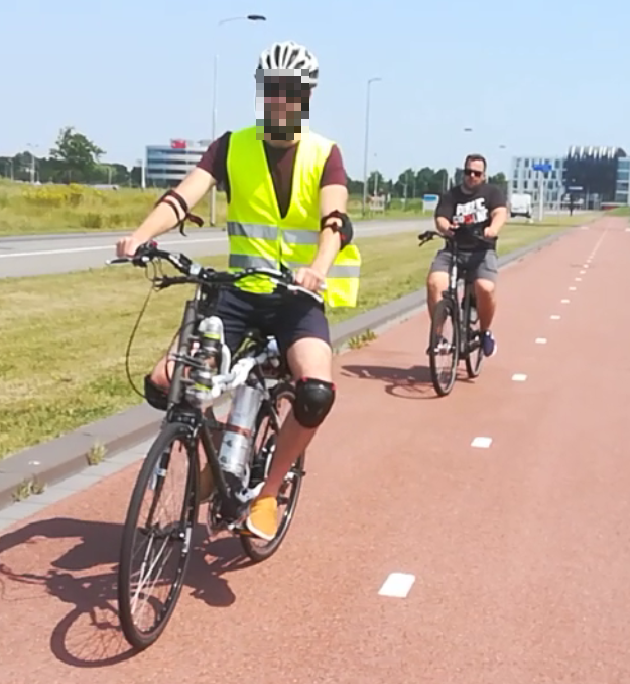
\includegraphics [width=0.6\textwidth]{images/steer_irf/steer_exp.png}
    \caption{Experimental trial performed across Heertjeslaan cycling path of TU Delft; Experiment coordinator cycling behind the steer-by-wire bicycle perturbing the subject through the mobile interface.}
    \label{steerexperiment}
    \end{figure}
\subsection{System Identification} 
The system identification procedure described in \cref{hapticFB} is also followed for this chapter. First a black box identification using the FIR model is conducted in order to  extract the linear relationship between disturbance and measurements effectively filtering intrasubject variability. This is done for both steering angle \ensuremath{\delta} and roll angle \ensuremath{\phi}. As will be later shown the intersubject variability is significant contrary to the lateral perturbation experiments. For this reason the gray box identification of the proposed rider control model is fitted on the individual responses of all participants instead of the median.
\subsubsection{Rider Control Model}
The full block diagram of the bicycle-rider system is shown in \cref{fig:intrinsic_block}. Process P consists of the bicycle dynamics given by \cref{eq:bikeEOM1,eq:bikeEOM2}. However since for this work the heading control is assumed to be insignificant, the equations of motion (EOM) are not extended with heading as an extra state. Additionally, the disturbance dynamics matrix \ensuremath{\boldsymbol{H}_d} changes in order to account for the fact that 100\% of the perturbation is transferred in the steering assembly, which means that \ensuremath{l_g=0} and \ensuremath{c_s=1}. Finally, element \ensuremath{{{M}_0}_{22}} of the mass matrix \ensuremath{\boldsymbol{M}_0} is increased by 0.21 \si{\kilogram.m^2} to account for the additional inertia induced by the passive rider \cite{schwab2012lateral}. 
\begin{figure}[h!]
    \centering
    % \captionsetup{justification=centering,margin=2cm}

    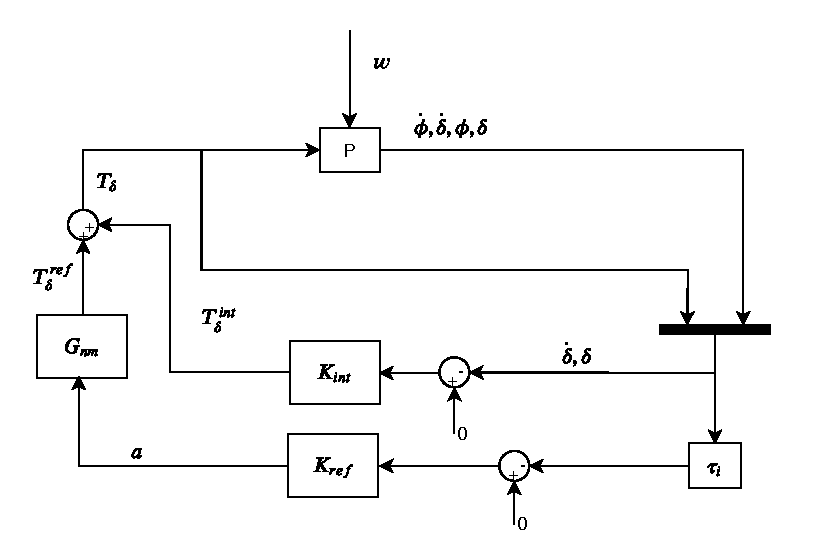
\includegraphics[width=\linewidth]{images/steer_irf/steering_block.pdf}
    \caption{Block diagram of the bicycle-rider system. System P consists of the bicycle dynamics. Controller blocks \ensuremath{K_{int}} and \ensuremath{K_{ref}} are pure gain blocks the parameters of which are estimated through gray box identification. The former works as the main reflexive controller with output the neural input \ensuremath{a}, while the latter is the intrinsic controller with output the intrinsic steering torque input \ensuremath{T^{int}_{\delta}} System \ensuremath{G_{nm}} represents the neuromuscular dynamics and its output is the reflexive steering torque input \ensuremath{T^{ref}_{\delta}}. Reflexive and intrinsic inputs combined give the complete steering torque input \ensuremath{T_\delta} to process P. All sensory inflow is delayed by \ensuremath{\tau_i} \si{\second} where \ensuremath{i} is the corresponding element of the sensory inflow vector.  }
    \label{fig:intrinsic_block}
\end{figure}
The full sensory signal vector including steering angle \ensuremath{\delta}, roll angle \ensuremath{\phi}, roll rate \ensuremath{\dot{\phi}}, steer rate \ensuremath{\dot{\delta}}, and steering torque \ensuremath{T_\delta} after being delayed by \ensuremath{\tau_i} are fed into the pure gain block \ensuremath{K_{ref}}. The produced neural input \ensuremath{a} is filtered through the neuromuscular dynamics block \ensuremath{G_{nm}} (see \cref{eq:gnmBLOCKA,eq:gnmBLOCKB}) to produce the reflexive component of the final control input to the process. As has been proven by motor control studies for the shoulder a significant part of the final forcing input is regulated through a different pathway; cocontraction \cite{schouten2008nmclab} . Cocontraction refers to the  simultaneous activation of antagonist muscles around a certain joint. This  provides the nervous system with a way to adapt the mechanical properties of the limb to changing task requirements without going through the neuromuscular lag and delay limitations of the reflexive response. In the model this is simulated by feeding \ensuremath{\delta} and \ensuremath{\dot{\delta}} to the pure gain block \ensuremath{K_{int}}.The state space representations of the aforementioned systems are discretized by zero order hold with a time step of 0.005 \si{\second}. For a look into how this time step affects simulation integration error refer to \cref{fig:convergence}. Additionally, in order to make the measured  and parametric ouptut signals comparable with simulation, they are resampled from 1000 \si{hz} to 200 \si{hz}.  For gray box identification 7 parameters in total are used. Five parameters for the five gains of \ensuremath{K_{ref}} and two parameters for the two gains of \ensuremath{K_{int}}.




The gains are estimated by fitting the model output into the non-parametric data-set by minimization of the cost function :
\begin{equation}
    V_{N}(\boldsymbol{\theta})=\frac{1}{N} \mathlarger{\mathlarger{\mathlarger{\sum}}}_{k=1}^{N}\left[0.16\frac{\left(\hat{y}^{\delta}_k(\mathbf{\theta})-y^\delta_k\right)^{2}}{\left(\overline{y}^{\delta}_k\right)^2}+0.8\frac{\left(\hat{y}^{\phi}_k(\mathbf{\theta})-y^\phi_k\right)^{2}}{\left(\overline{y}^{\phi}_k\right)^2}+0.04\frac{\left(\hat{y}^{T_\delta}_k(\mathbf{\theta})\right)^2}{\left(\overline{y}^{T_\delta}_k\right)^2}\right]
    \label{eq:cost2}
    \end{equation}


where \ensuremath{\boldsymbol{\theta}} is a vector containing all the free parameters, \ensuremath{\hat{y}^{\delta}} and \ensuremath{\hat{y}^{\phi}} are the outputs of the simulation for the measured external disturbance \ensuremath{w} and the vector of parameters  \ensuremath{\boldsymbol{\theta}} for steer angle \ensuremath{\delta} and heading angle \ensuremath{\phi}  respectively, while \ensuremath{y^\delta} and \ensuremath{y^\phi} are the outputs of the non-parametric model. inally \ensuremath{\overline{y}^{\delta}_k,\overline{y}^{\phi}_k,\overline{y}^{T_\delta}_k} are the absolute maximum allowable values of the non-parametric signals and are equal to 0.4 \si{\radian}, 0.4 \si{\radian}, 10 \si{N.m} respectively.

The first two terms  of the cost function are trying to match the steering and roll  response of the parametric model with that one of the non-parametric model, while the third on minimizes the amount of input torque generated in order to produce the best possible fit while maintaining minimal control effort. The weights are chosen heuristically. For optimization the genetic algorithm with a fitness limit of 0.03 is first  used in order to produce a good starting parameter vector for gradient descend algorithm to take over, which finally finds the closest possible estimate of the global minimum. For the genetic algorithm a crossover fraction of 0.85  along with a population size 10 times the length of the parameter vector is used. 

To assess fitting performance the \ensuremath{\mathrm{VAF}} for \ensuremath{\phi} and \ensuremath{\delta} is used as defined by \cref{eq:VAF}.
\section{Results}
\subsection{Non parametric Model}
The level of fit of the non-parametric model to the measured signals as a function of forward speed is seen in \cref{fig:FIT_FIR} for all 14 participants. The \ensuremath{\mathrm{VAF}} is significantly low for both outputs which indicates that there is significant variability of the individual rider response within the trials; especially for the lowest forward speed level. 
\begin{figure}[h!]
    \centering
    % \captionsetup{justification=centering,margin=2cm}

    \includegraphics[width=\linewidth]{images/steer_irf/FIT_irf_steer.eps}
    \caption{Box plot of the  \ensuremath{\mathrm{VAF}} between measurements of \ensuremath{\delta} and \ensuremath{\phi} and non-parametric outputs \ensuremath{y^\delta} and \ensuremath{y^\phi} respectively for all forward speed levels.}
    \label{fig:FIT_FIR}
\end{figure}

The impulse response functions produced by fitting the FIR model into the measured data for roll and steer is seen in \cref{fig:IRF_all}. The results show great variability amongst participants.
\begin{figure}
    \centering
    \begin{subfigure}[b]{\textwidth}
        \centering
        \makebox[\textwidth][c]{\includegraphics[width=1.1\linewidth]{images/steer_irf/roll_irf_steer.eps}}
        \caption{}
        \label{fig:IRF_phi}
    \end{subfigure}
    \begin{subfigure}[b]{\textwidth}
        \centering
        \makebox[\textwidth][c]{\includegraphics[width=1.1\linewidth]{images/steer_irf/steer_irf_steer.eps}}
        \caption{}            
        \label{fig:IRF_delta}
    \end{subfigure}
    \caption{Impulse response functions estimates produced by the FIR model  roll (a) and steer(b) for all forward speed levels. The closer a response is to the mean rider the more red  the lines.}
    \label{fig:IRF_all}
 \end{figure}
\subsection{Parametric Model}
The proposed rider control manages to match the non-parametric outputs with an overall good level of fit between both roll and steer (see \cref{fig:FIT_model}). The roll  shows comparatively lower fit performance but increases as forward speed gets bigger. This indicates some potential bicycle model inaccuracy which  leads to mismatch in steer-roll coupling dynamics for low speeds.   In \cref{fig:model12,fig:model34}, the response of the first participant is compared with the simulated rider model output and the results show great similarity even for the control input.
\begin{figure}
    \centering
    \begin{subfigure}[b]{\textwidth}
        \centering
        \makebox[\textwidth][c]{\includegraphics[width=1.4\linewidth]{images/steer_irf/param_signals_25.eps}}
        \caption{}
        \label{fig:model1}
    \end{subfigure}
    \begin{subfigure}[b]{\textwidth}
        \centering
        \makebox[\textwidth][c]{\includegraphics[width=1.4\linewidth]{images/steer_irf/param_signals_38.eps}}
        \caption{}            
        \label{fig:model2}
    \end{subfigure}
    \caption{Comparison between parametric model output, non-parametric model ouput and measured signals for the two lowest speed levels for the first participant.}
    \label{fig:model12}
 \end{figure}
 \begin{figure}
    \centering
    \begin{subfigure}[b]{\textwidth}
        \centering
        \makebox[\textwidth][c]{\includegraphics[width=1.4\linewidth]{images/steer_irf/param_signals_46.eps}}
        \caption{}
        \label{fig:model3}
    \end{subfigure}
    \begin{subfigure}[b]{\textwidth}
        \centering
        \makebox[\textwidth][c]{\includegraphics[width=1.4\linewidth]{images/steer_irf/param_signals_55.eps}}
        \caption{}            
        \label{fig:model4}
    \end{subfigure}
    \caption{Comparison between parametric model output, non-parametric model ouput and measured signals for the two highest speed levels for the first participant.}
    \label{fig:model34}
 \end{figure}

 \begin{figure}[h!]
    \centering
    % \captionsetup{justification=centering,margin=2cm}

    \includegraphics[width=\linewidth]{images/steer_irf/param_fit_box.eps}
    \caption{Box plot of the  \ensuremath{\mathrm{VAF}} between non-parametric output  of \ensuremath{\delta} (right) and \ensuremath{\phi} (left) and  parametric outputs \ensuremath{\hat{y}^\delta} and \ensuremath{\hat{y}^\phi}  for all forward speed levels.}
    \label{fig:FIT_model}
\end{figure}
The seven gains estimated for all participants are shown in \cref{fig:gain_plots_steer,tb:steer_gains}. Approximate linear trends are noted for all gains. Additionally, the intersubject variability for the forward speed level of 2.6 \si{\meter\per\second} is disproportionally higher than the rest, as noted by the much larger standard deviation in all gains. In \cref{fig:param_input} the decomposition of the input signal as the rider responds to the first perturbation of each forward speed level's run is shown. The intrinsic torque \ensuremath{T_\delta^{int}} initially acts as expected countering part of the perturbation torque, after that however it acts as a  regulatory mechanism, mirroring the reflexive response.

    \begin{table}[]
        \caption{Mean and standard deviation of all controller gains as estimated for the 14 participants.}
        \resizebox{\columnwidth}{!}{%
        \begin{tabular}{lllllllllllllll}
        $v\;\;\;(\si{m.s^{-1}})$                       & \multicolumn{2}{l}{$K_{\dot{\phi}}\;\;\;\;(\si{kg.m^2.s^{-2}})$} & \multicolumn{2}{l}{$K_{\dot{\delta}}\;\;\;\;(\si{kg.m^2.s^{-2}})$} & \multicolumn{2}{l}{$K_{{\phi}}\;\;\;\;(\si{kg.m^2.s^{-1}})$} & \multicolumn{2}{l}{$K^{ref}_{{\delta}}\;\;\;\;(\si{kg.m^2.s^{-1}})$} & \multicolumn{2}{l}{$K_{T_{\delta}}\;\;\;\;(-)$} & \multicolumn{2}{l}{$K^{ref}_{\dot{\delta}}\;\;\;\;(\si{kg.m^2.s^{-2}})$} & \multicolumn{2}{l}{$K^{int}_{{\delta}}\;\;\;\;(\si{kg.m^2.s^{-1}})$} \\ \cline{2-15} 
                                  & $\mu$                          & $\sigma$                        & $\mu$                          & $\sigma$                          & $\mu$                        & $\sigma$                      & $\mu$                           & $\sigma$                           & $\mu$                 & $\sigma$                & $\mu$                             & $\sigma$                             & $\mu$                           & $\sigma$                           \\ \hline
        \multicolumn{1}{l|}{2.68} & -55.10                         & 24.88                           & 1.66                           & 1.72                              & -89.90                       & 114.97                        & 6.60                            & 8.14                               & -0.99                 & 0.29                    & 10.14                             & 2.57                                 & 25.89                           & 24.41                              \\
        \multicolumn{1}{l|}{3.68} & -37.16                         & 12.15                           & 3.81                           & 2.04                              & -48.48                       & 14.75                         & 8.82                            & 8.94                               & -1.04                 & 0.05                    & 9.54                              & 2.72                                 & 30.19                           & 9.36                               \\
        \multicolumn{1}{l|}{4.49} & -29.57                         & 8.52                            & 4.27                           & 1.25                              & -43.72                       & 17.69                         & 12.13                           & 11.47                              & -1.02                 & 0.08                    & 8.97                              & 2.61                                 & 39.82                           & 14.24                              \\
        \multicolumn{1}{l|}{5.63} & -23.72                         & 7.26                            & 5.67                           & 2.51                              & -37.68                       & 16.46                         & 13.40                           & 14.29                              & -1.00                 & 0.08                    & 7.79                              & 2.47                                 & 52.89                           & 15.44                             
        \end{tabular}%
        }
        \label{tb:steer_gains}
        \end{table}
\begin{figure}[h!]
    \centering
    % \captionsetup{justification=centering,margin=2cm}

    \includegraphics[width=\linewidth]{images/steer_irf/param_gains_plot.eps}
    \caption{Mean of estimated gains as a function of forward speed. Error bars indicate one standard deviation of the mean.}
    \label{fig:gain_plots_steer}
\end{figure}

\begin{figure}[h!]
    \centering
    % \captionsetup{justification=centering,margin=2cm}

    \includegraphics[width=\linewidth]{images/steer_irf/param_input.eps}
    \caption{Steering torque response to the first perturbation (dashed yellow) of the first participant as a function of time. The input is decomposed in the intrinsic component(orange) and the reflexive component (blue). }
    \label{fig:param_input}
\end{figure}
\section{Discussion}
As seen by \cref{fig:FIT_FIR} the \ensuremath{\mathrm{VAF}} is relatively low especially for roll angle \ensuremath{\phi} which means that significant variations in rider response within the same trial are present. This shows that the participants adapted their strategies as the trial went forward, consciously choosing to be more compliant or stiff depending on the situation. Despite the fact the experimental procedure was conducted in a much more proper manner than in the lateral perturbation experiment, meaning that subjects could in no way expect the bilateral perturbations sent through the wireless interface, the nature of the steering perturbation is such that allowed the participants to damp out big parts of the disturbance through cocontraction. One of the goals of this study is to investigate  the balance between reflexive response and cocontraction. However since we assume the bicycle to be linear time invariant for fixed forward speeds we expect consistent rider behavior as a function of speed, which means that the large intrasubject variability can not be captured by the model.

The lowest forward speed level displays disproportional level of variability as shown by the huge standard deviation margins across estimated parameters (see \cref{fig:gain_plots_steer}). This indicates that the intersubject variability present for that speed level is significantly higher. This could be an after effect of the the fact that the lowest speed level was always the first run. Although trial runs were conducted beforehand at various speed levels, some participants may not have adapted to the system completely which caused them to exhibit significant variance in their response.

Negative proportional and derivative gains for roll angle \ensuremath{\phi} indicate the reliance on the so called "steer into the fall" mechanism.   Modulation of steering stiffness is dominated by cocontraction as the reflexive \ensuremath{K_\delta} stays close to zero across speed levels (see \cref{fig:gain_plots_steer}). An increasing reliance on intrinsic steering stiffness as speed increases is noted. On the other hand, the intrinsic modulation of steering damping is lessened as speed increases, in favor of the reflexive pathway (see \cref{fig:gain_plots_steer}). What is more interesting however is the way the intrinsic and reflexive components of the control input interact with each other in order to create the final applied rider torque. The torque generated by cocontraction initially acts as a way to lessen the  impact of the perturbation as seen by the first few milliseconds in the intrinsic signal of \cref{fig:param_input}. During optimization of the parameters the intrinsic gains are tuned in order to best counter initial impact on the steering states by the perturbation. However since we assume a time invariant  system the same parameters act on the later milliseconds as well, creating the weird mirroring effect between reflexive and intrinsic components. This upon initial observation seems counter intuitive since it seems that the reflexive controller is fighting against the intrinsic one. The reason why this happens is the fact that the reflexive response is dominated by the "steer into the fall" strategy of control, while the intrinsic mechanism is trying to achieve  steering angles and rates equal to zero. In reality the intrinsic response of the rider is not time invariant. At the first few milliseconds of the perturbation cocontraction is active while afterwards when the rider needs to actually balance the bike by steering into the fall cocontraction is lessened and the reflexive is the main mechanism of control.  In a more realistic model this behavior should be captured.
\section{Conclusions}
In conclusion the rider model created manages to achieve a good level of fit and simultaneously captures the significance of the intrinsic response when countering steering torque perturbations. A high level of intersubject variability is exhibited. The hypothesis that this variability is in fact due to the modulation of admittance in the shoulder joint is strongly indicated. Despite all that,  the assumption that for constant speeds the system is time invariant does not seem to hold ground as noted by the irregular effect of cocontraction in the later stages of the rider  response.

% \chapter{Methods}
\label{methods}


In order to answer the research question posed, Google scholar was  used as the main tool of literature research. It proved to be the search engine with the most relevant and extensive literature.


In order to understand how a rider can be modelled as a controller, an understanding of single track vehicle dynamics is paramount. For that reason the first step was to seek literature that extensively describes the equations of motion of single track vehicles and analyses the unique problem arising from their inherent instability in low speeds. Search terms: “bicycle”, “dynamics”, “stability” , “motorcycle”, “equations + motion”, “eigenvalue + analysis”, “linear” , “non-linear”  were used.


\par
The next step was to find any published reviews on the subject of rider control for bicycles and motorcycles. The reviews of Kooijman et al.\cite{kooijman2013review}, Popov et al.\cite{popov2010review} and the bibliography review from Moore’s PHD thesis \cite{moore2012human} proved the most substantiated and extensive on the subject. A distinction was made between articles that were simply looking at bicycle and motorcycle control in general (ex. robot bicycles) and those that specifically tried to model the human controller. The latter  were more thoroughly visited. 

\par
In order to fill the gaps of more recent literature, an additional search on google scholar was conducted. The search was done by looking at papers involving keywords such as “rider control” , “rider identification” , “controller”, “optimal”, “McRuer”, “cybernetics”. For bicycle control results were filtered by looking at articles that directly cited the work of Meijaard et al. \cite{meijaard2007linearized} in bicycle dynamics, while for motorcycles results were filtered by looking at direct citations of Sharp’s work in motorcycle dynamics \cite{sharp1971stability}. These two articles involve the most prominent versions of linearized equations of motion for single track vehicle, so they are bound to be mentioned in any modern take on rider modelling.

Finally a search outside the scope of the problem was done looking at how the human controller is modelled in other motor related tasks. Search keywords included : “sensory-motor + integration” , “human + optimal + controller”, “Wolpert”, “Inverse + model”, “Internal + Model”, “feed-forward + control”.

All the relevant articles were stored in a database. If the article involved some form of control that the authour found unfamiliar, further research on the subject was conducted. These included fuzzy logic control, intermittent control and  model predictive control. After reading into the abstacts and conclusions of each article, an initial assesment was made on the relevancy of the work. Depending on that evaluation, a more extensive reading of the methods of some of the articles was done.
% \chapter{Results}
\label{results}

\section{Bicycle dynamics and stability} \label{sub:bicycle}
This literature review aims to answer the research question regarding the validity of available rider models of single track vehicles. This includes both bicycles and motorcycles, as the list of bicycle rider models is not extensive enough. The plant is a necessary part of every closed loop control system and in this section the prevalent  way of expressing the dynamics and stability of a bicycle is described so as to better understand  what the controllers in the later sections are trying to actually control.
\subsection{The linearized Whipple-Carvalho bicycle model}
Bicycles are  very reliable transport vehicles and are considered the most efficient man powered form of transportation. Since the inception of the safety bicycle not much has changed with regards to the design of the two wheeled vehicle.   Bicycle design has been based on tinkering rather than equations which has resulted in little mathematical scrutiny in the available bicycle analyses. When trying to design a controller for a bicycle, a model that accurately describes its dynamics and kinematics is required but until 2007 there was no consensus on a set of equations that do that, so research on rider control for bicycles was hardly attempted. This changed when Meijaard et al.\cite{meijaard2007linearized}  developed a set of linearized equations of motion for the Whipple-Carvalho bicycle  model (fig \ref{fig:figure2}).\par
\begin{figure}[ht]
    \centering
    \includegraphics[scale=0.3]{images/figure3_1.png}
    \caption{ The Whipple-Carvalho bicycle model consists of four rigid bodies: rear wheel R, rear frame B, front frame H and front wheel F connected via hinges. The center of mass locations are expressed relative to the x - and z -coordinates shown (with origin at P and y pointing towards the reader). The other parameters shown are the steer axis tilt \ensuremath{\lambda}, wheelbase \ensuremath{w} and trail \ensuremath{c}. The model at its most expanded form is described by 25 parameters.\cite{meijaard2007linearized}}
    \label{fig:figure2}
\end{figure}


\vbox{%
    For  the equations of motion to be derived several assumptions were made by Meijaard  et al.\cite{meijaard2007linearized}:

    \begin{enumerate}
        \item The rider is rigidly connected to the rear frame with the mass of the arms included in the mass.
        \item The contact between tire and ground is modelled as a non-slipping rolling point-contact, meaning
              that wheels have an ideal rotation without lateral slip.
        \item Friction between moving parts and pedaling forces is neglected. Thus, the total energy of the
              system is constant.
        \item The bicycle is moving with constant forward velocity.
    \end{enumerate}}
\par
In order to understand the derived equations of motion a consideration must be made with regards to the configuration space and the velocity space of the model. The benchmark bicycle model derived is defined by 25 parameters. However, as a result of holonomic constraints (hinges and ground contacts) and non-holonomic constraints (non-slipping rolling contacts), its accessible configuration space can be reduced to 7 parameters. Coordinates \ensuremath{x_{P}} and \ensuremath{y_{P}} represent the translational position of the rear wheel point P, \ensuremath{\delta} is the steer angle, \ensuremath{\theta_{F}} and \ensuremath{\theta_{R}}  are the front and rear wheel angles respectively. Finally \ensuremath{\phi}  represents the lean angle about the x axis while \ensuremath{\psi}  represents the yaw rotation about the z axis. All this is depicted in figure \ref{fig:figure3}.
\begin{figure}[ht]
    \centering
    \includegraphics[scale=0.3]{images/figure3_2.png}
    \caption{Depiction of the benchmark bicycle in 3D. The cans represent a hinge between two rigid bodies. Multiple cans in series denote multiple degrees of freedom and the order of rotation.\cite{meijaard2007linearized}}
    \label{fig:figure3}
\end{figure}
\par
As it turns out some of the configuration variables do not appear in any of the equations of motion of the different parts. These so-called cyclic or ignorable coordinates are: the location of the bicycle on the plane (\ensuremath{x_{P}}, \ensuremath{y_{P}}), the heading of the bicycle \ensuremath{\psi} and the rotations (\ensuremath{\theta_{R}}, \ensuremath{\theta_{F}}) of the two wheels relative to their respective frames \cite{meijaard2007linearized}. Additionally due to a symmetry of the bicycle design and the lateral equations of motion, a  first order decoupling between forward and lateral dynamics exists \cite{meijaard2007linearized}. This means that the equations governing forward movement can be ignored when examining lateral dynamics like bicycle stabilization and vice versa. In conclusion, the three independent degrees of freedom that define the equations of motion are the  forward speed \ensuremath{\nu},  the lean angle \ensuremath{\phi} and the  steering angle \ensuremath{\delta} (figure \ref{fig:figure3}).
\subsection{The linearized equations of motion}
Keeping in mind the above considerations Meijaard et al.\cite{meijaard2007linearized} managed to formulate a set of three linearized equations that each describe a degree of freedom. The first is a first order differential equation that describes the forward speed as shown in equation \ref{eq:equation1}\cite{meijaard2007linearized}.
\begin{equation}
    \left[r_{R}^{2} m_{T}+I_{R y y}+\left(\frac{r_{R}}{r_{F}}\right)^{2} I_{F y y}\right] \ddot{\theta}_{R}=T_{\theta_{R}}
    \label{eq:equation1}
\end{equation}
where \ensuremath{I}, \ensuremath{r} and \ensuremath{m} denote inertia, radius and mass respectively of the rigid body defined in the subscript. Also \ensuremath{T_{\theta_{R}}} denotes the torque applied to the rear wheel in the direction of \ensuremath{\theta_{R}}.
\par
For the two remaining degrees of freedom the lean angle(\ensuremath{\phi}) and the steer angle (\ensuremath{\delta}) they found two second-order differential equations that are coupled and are given by equation \ref{eq:equation2}\cite{meijaard2007linearized}.
\begin{equation}
    \mathbf{M} \ddot{q}+v \mathbf{C}_{1} \dot{q}+\left[g \mathbf{K}_{0}+v^{2} \mathbf{K}_{2}\right] \mathbf{q}=\mathbf{f}
    \label{eq:equation2}
\end{equation}
where \ensuremath{q} is a vector containing the roll and steer angles, \ensuremath{f} is a vector containing the roll and steer torques, \ensuremath{g} is the gravitational acceleration and \ensuremath{\mathbf{M},\;v\mathbf{C}_{1},\;g \mathbf{K}_{0}+v^{2} \mathbf{K}_{2}} are the "mass", "damping" and "stiffness" ratios in matrix form respectively.

When talking about bicycle stability and control, equation \ref{eq:equation1} is often ignored as the task of pedaling is often removed from the problem so as to focus on pure roll stabilization. For control purposes it is convenient to express the bicycle equation \ref{eq:equation2} in state-space form . The state-space representation is:
\begin{equation}
    \dot{\mathbf{x}}=\mathbf{A} \mathbf{x}+\mathbf{B} \mathbf{f}
\end{equation}
\begin{equation}
    \mathbf{y}=\mathbf{C} \mathbf{x}+\mathbf{D} \mathbf{f}
\end{equation}
where matrices \ensuremath{A,B,C,D} are defined by:
\begin{equation}
    \mathbf{A}=\begin{bmatrix}
        -\mathbf{M}^{-1}v\mathbf{C}_{1} & -\mathbf{M}^{-1}(g \mathbf{K}_{0}+v^{2}\mathbf{K}_{2}) \\
        {\mathbf{I}}                    & {\mathbf{0}}
    \end{bmatrix} , \mathbf{B}=\left[ \begin{array}{c}{\mathbf{M}^{-1}} \\ {\mathbf{0}}\end{array}\right] ,
    \mathrm{C}=\begin{bmatrix} {\mathbf{0}} & {\mathbf{I}}
    \end{bmatrix} , \mathrm{D}=[\mathbf{0}]
\end{equation}
\par
By finding the eigenvalues of matrix \ensuremath{A} one can begin asking questions regarding the stability of the system. Meijaard et al. \cite{meijaard2007linearized} found the eigenvalues for different forwards speeds and managed to determine the region in which the uncontrolled benchamark bicycle was stable. In figure \ref{fig:figure4} the four eigenvalues are plotted in a forward speed range \ensuremath{0<v<10\; ms^{-1}}. The region that is defined when the real part of the weave eigenvalue becomes negative and the capsize eigenvalue has not crossed the zero threshold yet is the stable region and corresponds to forward speeds  \ensuremath{4.3\lessapprox v \lessapprox 6\; ms^{-1}}. When designing a controller  the input signals \ensuremath{f} are tasked with influencing the poles of the characteristic polynomial and moving the system from the unstable region to a stable one.

\begin{figure}[ht]
    \centering
    \includegraphics[scale=0.6]{images/figure3_3.png}
    \caption{Root locus plot of the benchmark bicycle. Bold black lines indicate the real part of the eigenvalues while dotted show the imaginary part.\cite{meijaard2007linearized}}
    \label{fig:figure4}
\end{figure}

Before exploring potential control options for the bicycle model described by the above equations, it is interesting to see to what extent is the model controllable. We know that the bicycles and motorcycles are controllable in reality but how well does this model capture reality is still a question.

To determine controllability of a dynamical system the reachability matrix :

\begin{equation}
    \mathbf{Q}=\left[\mathbf{B}, \mathbf{A B}, \mathbf{A}^{2} \mathbf{B}, \cdots, \mathbf{A}^{k-1} \mathbf{B}\right]
    \end{equation}
must be full rank. When the matrix rank is equal to the number of states of the system then the system is controllable by inputs \ensuremath{f}. By taking the determinant and then solving the equation:
\begin{equation}
    det\; \mathbf{Q} = \mathbf{0}
\end{equation} 
the forward velocities that result in an uncontrollable system can be found. Schwab et al. in \cite{schwab2010controllability} isolated the control inputs and found that a Whipple like bicycle with the an extended rider model can be controlled by either lean or steer torque for the practical range of 1 to 10 \ensuremath{\frac{m}{s}}. Although some forward speeds that result in a zero determinant exist they were either extremely close to zero or part of a stable mode so they concluded that they are of no concern.

\section{Rider modelling} \label{sub:rider}
When trying to model the rider of  single track vehicles some important considerations have to be made. As discussed in earlier sections the most important distinction comes from the consideration of which rider control inputs are implemented. When the focus of the model is purely on the steer control the rider body can be modelled as a simple fixed rigid body attached to the seat post of the vehicle as was implemented by Whipple \cite{whipple1899stability}. When the lateral body motion is considered significant control input, the rider  is often modelled as a two piece body. The lower part is still fixed on seat post but the upper part is modelled like an inverted pendulum. As a connection between the two, a spring dumper system is often placed \cite{aoki1999effectiveness,astrom2005bicycle,seffen1999bicycle}. The dynamics of  the combined system are expressed as extensions of the vehicle model.\par
Even when examining purely steer control, a distinction can be made between the types of control the rider performs, position(angle) or force (torque). For automobiles it is widely accepted that the driver controls the vehicle with position control \cite{plochl2007driver,guo1993modelling}. However for single track vehicles, where riders move the handlebars to a much lesser degree than in automobiles and where also the corner counter steer effect is present, a distinction cannot be easily made between which types of control the rider employs so models in literature  have explored both avenues.\par
The final important aspect that defines a rider model is the control task. For rider models of single track vehicles in literature, authors distinguish between  the stabilization task and the path following task.  Stabilization tasks  are used  when  trying to understand the effort applied by the rider in order to keep the vehicle from falling over. On the other hand  path following tasks are employed when the goal is to follow a set course. There are two types of models that are involved with path following tasks. The first is compensatory where the rider adjusts his position in order to minimize the difference between the refence trajectory and his current position. The second involves the concept of preview, this methods enhances the compensatory model by introducing a look ahead of the upcoming path. The decision at each moment is determined by a weighted average of the feedback and feedforward controller.

Given what was found in literature the controllers describing rider behavior were characterized by the above observations. This includes whether the model describes pure steer control (angle or torque) or implements some compensation for rider body dynamics. Also distinctions were made for models that tackled stabilization tasks or path following tasks. The models were also categorized depending on the underlying control theory  approach their authors employed. First there is the classical control approach which was most prominently applied to the airplane pilot behavior modelling. The second is the optimal control framework where the rider is assumed to be an optimal controller. This approach tries to introduce a weighted average between the effort put by the rider and the performance in the given task. Simulating the human controller as an optimal controller is a pathway that has been extensively explored in modelling of motor related tasks \cite{baron1984adaptive}. Finally all the rest were grouped under the banner of other methods. These include fuzzy logic, intermittent control, neural networks and controllers based on inverse dynamics.
\subsection{Classical control system design} \label{ch:classical}

The first attempt to model the human controller was done by McRuer for advancing the understanding of aircraft pilot control \cite{mcruer1967manual,mcruer1967manual2,mcruer1959human} in a post-war world where the study of cybernetics was blowing up. The general idea of the McRuer model is that the human controller tries to adapt so that the open loop system (fig.\ref{fig:figure5}) behaves like a first order integrator.
\begin{figure}[ht]
    \centering
    \includegraphics[scale=0.6]{images/figure3_4.png}
    \caption{Block diagram of a typical human-machine system control loop as described by McRuer, where \ensuremath{i} is the reference control value, \ensuremath{m} is actual control value; \ensuremath{e} is the control value error, \ensuremath{Y_e^c} is the human controller transfer function, \ensuremath{c} is rider output control variable and \ensuremath{Y_c^m} is the machine transfer function.\cite{kooijman2013review}}
    \label{fig:figure5}
\end{figure}
\par
For example if the pilot tries to control a task with first order dynamics (1st order integrator) then the human would act like a simple gain, leading to a first order integrator open loop system. McRuer found that this behavior is present for compensatory task in the vicinity of the gain cross over frequency, \ensuremath{\omega_c}. Cross-over frequency is the frequency that the open loop magnitude bode  plot crosses the unity line. He also introduced a time delay which comes from the inherent neuromuscular limitations of the human body. The formula for the open loop transfer function is shown below:
\begin{equation}
    Y_{e}^{c} Y_{c}^{m}=\frac{\omega_{c}}{j \omega} e^{-j \omega \tau}
    \label{eq:equation3}
\end{equation}
where \ensuremath{Y_e^c} is the pilot transfer function, \ensuremath{Y_c^m} is the transfer function describing the dynamics of the controlling task and \ensuremath{\tau} is the time delay. Equation \ref{eq:equation3} also known as the McRuer cross over model was enhanced to include further limitations of the human controller leading to equation \ref{eq:equation4} which is known as the McRuer precision model. This model makes the human a lead-lag system with time delay and limits the systems that a human operator can control.

\begin{equation}
    Y_{e}^{c}=K_{p} \frac{\left(T_{L} j \omega+1\right)}{\left(T_{I} j \omega+1\right)} e^{-j \omega \tau}
    \label{eq:equation4}
\end{equation}
where \ensuremath{T_L} is the time lead and \ensuremath{T_l} is the time lag.

\par
 The principles of this study were modified and implemented in numerous human controller modelling attempts for various tasks, from automobiles to tele-manipulators. Rider Models with the classical control approach were not deemed appropriate by many authors due to the multi loop control nature of single track vehicle stabilization and path following. This is why, not many of these types of models exist. However, recent attempts  by Hess\cite{hess2012modeling} and Schwab et al.\cite{schwab2013} have shown promising results.

\underline{\textbf{The Stasem and van Lunteren controller\cite{van1970influence}}}
\newline

Their model assumed angle control. It consisted of a PD controller with a time delay. The input was the frame roll angle and the output was the steer angle and upper body lean angle. They managed to get data for the system identification by creating a bicycle simulator. The goal of the study was to determine the effect of drugs on rider behavior by reflecting on the changes of the estimated parameters of the model. Unfortunately the experiments were conducted only on one speed (4.17 m/s) and the simulator provided no visual feedback. An interesting finding of this early study was the fact that path following and stabilization tasks did not seem to affect each other that much, as when the path following task was introduced  the proportional and derivative gains of the stabilization control loop did not alter significantly.

\bigbreak

\underline{\textbf{The CALSPAN group controller\cite{roland1971digital,roland1972bicycle,roland1973computer}}}
\newline

Following in Stasem’s and van Lunteren’s footsteps, Roland and Lynch developed a bicycle stability and path following controller but with the assumption that the output of said controller are torques, in comparison with the Delft model where angle control was assumed. The controller consisted of an inner loop which was responsible for stabilization and an outer loop which tried to minimize lateral deviation to achieve the tracking of a given trajectory.  The stabilization controller had the roll angle ,roll rate and roll acceleration as inputs  and consisted of a derivative, a proportional and an integral part (PID) with a time delay. The outputs were both the lean and steer torques. For the outer loop tracking controller, the input was the lateral deviation from the desired path and had an extra roll angle as output which was then added to the existing roll angle measured from the plant.  The only real experiments the model was used for were conducted by Rice\cite{rice1978rider} but the results did not compare well with the experimental data.

\bigbreak

\underline{\textbf{Weir’s rider model \cite{weir1973manual}}}
\newline

Weir developed a controller for Sharp’s motorcycle model\cite{sharp1985lateral} while being fully aware of McRuer’s prior work ,as he worked with him on many of his experiments. He assumed that torque control was far more plausible than angle control. His model is similar to the CALSPAN group model as it tries to tackle both stabilization and path following with lean torque and steer torque as plant inputs. However he tried to maintain single input single output transfer functions for his inner loops. He found from experimental data that  the best ones were the roll angle to steer torque due to the high gain and phase margins. His model is depicted in figure \ref{fig:figure6}. In contrast with the CALSPAN group controller Weir’s controller includes an additional  feedback loop for the control of the heading angle. The tracking controller output was also the heading angle and not the roll angle used by Roland et al.
\begin{figure}[ht]
    \centering
    \includegraphics[scale=1.0]{images/weir_block.png}
    \caption{Weir's motorcycle rider model for Sharp’s motorcycle model. Plant outputs : lateral deviation (\ensuremath{y_l}), heading angle (\ensuremath{\Psi}), roll angle (\ensuremath{\Phi}),Rider controller inputs: plant ouputs ,reference path (\ensuremath{y_{l_c}}),Plant Inputs: steer torque (\ensuremath{T}), upper body lean torque (\ensuremath{\Phi_R}),  Trasfer Functions: tracking controller (\ensuremath{Y^{\Psi_C}_{y_l}}), heading controller  (\ensuremath{Y^{\Phi_R}_{\Psi}}), roll controller(\ensuremath{Y^{T}_{\Phi})})}
    \label{fig:figure6}
\end{figure}
\par
Eaton in his PHD thesis\cite{eaton1987man}  tried to validate the Weir model with experimental data. However he made some changes in order to get better results. Primarily he  focused on the inner roll stabilization loop and excluded the body lean torque as control input.
\par
Prem and Good\cite{prem1984rider} also worked with the Weir model in order to make observations about the steering behavior of novice motorcycle riders. In their experimental dataset they found that there is strong coupling between steering and rider upper body leaning inputs, so a modification was made on the Weir model introducing exactly that. They found that the extra coupling increases the gain of the transfer function allowing the large rider lean to roll angle error gain values to drop to more realistic levels. They also found comparable tracking capabilities with the stabilization ones and they concluded that although their model resulted in lower stability margins it resulted in far smaller upper body lean motions which in in experienced riders was always present.

\bigbreak

\underline{\textbf{Hess’s  rider model\cite{hess2012modeling}}}
\newline

In a recent attempt by Hess et al. to introduce a task independent handling qualities metric for bicycle control, he developed a model using the classical control approach. The behavior first observed by McRuer’s crossover model  can be captured by a variety of theoretical control structures from simple dynamics to complex neuromuscular models\cite{hess1984effects}. Hess believed that, the simpler models can often capture much of the essential dynamics in human-machine systems such as the bicycle-rider one. So he developed a model similar in nature to Weir’s and based on the foundation of the early McRuer experiments. The controller is using torque control and takes only the steer torque as input. More specifically, it has an inner roll stabilization loop, which can be seen in \ref{fig:figure7} ,and an outer heading and lateral deviation control  loop ,which is depicted in figure \ref{fig:figure8}.
\begin{figure}[ht]
    \centering
    \includegraphics[scale=0.4]{images/hess_roll.png}
    \caption{The inner loop structure of the Hess Rider Controller with steer angle \ensuremath{\delta}, roll rate \ensuremath{\dot{\phi}}, and roll angle \ensuremath{\phi} feedback loops. The inner loops are closed with sequential gains starting with the proprioceptive steer angle loop, followed by the vestibular roll rate loop, and the visual roll angle loop. The steer angle loop captures the force/feel  we use while interacting with the handlebars.\cite{moore2012human}}
    \label{fig:figure7}
\end{figure}
\begin{figure}[ht]
    \centering
    \includegraphics[scale=0.45]{images/hess_lat.png}
    \caption{The outer loop structure of the control system with the heading angle \ensuremath{\psi} and lateral deviation \ensuremath{y_q} being fed back.\cite{moore2012human}}
    \label{fig:figure8}
\end{figure}
\par
The model in essence contains five gain values for the five different feedback loops and two fixed second order filter coefficients determined by the neuromuscular system of the human along with a preview time parameter.  Although an attempt was made by Moore \cite{moore2012human} the model has yet to be experimentally validated.
\bigbreak
\underline{\textbf{The Schwab and de Lange model \cite{schwab2013}}}
\newline

First introduced in the master thesis of de Lange in 2011 and later published in 2014, this model is one of the most recent attempts to model the behavior of the bicycle rider which has been indirectly validated through system identification of its parameters. The particular model only examines the stabilization task and assumes  torque control. They also considered the upper body lean torque to be insignificant for stabilization purposes, so the only internal input of the plant was the steer torque. The input of the controller was the steer angle and roll angle of the bicycle. The controller consisted of a proportional, an integrative, a first- and a second-order derivative component acting on both the roll and steer angles (\ensuremath{K_\phi} and \ensuremath{K_\delta} respectively). While eight parameters were initially used they were later reduced by keeping only the ones that showed significant impact on the variance accounted for. This created a more realistic model of the rider and removed any potential concerns of overfitting the dataset. The controller is depicted in figure \ref{fig:figure9}.

\begin{figure}[ht]
    \centering
    \includegraphics[scale=0.55]{images/deLange_block.png}
    \caption{Block diagram of the inner control structure of controller \ensuremath{K}, with roll and steering angle feedback gains \ensuremath{K_\phi} and \ensuremath{K_\delta}, time delay \ensuremath{G_\tau}, neuromuscular lag \ensuremath{G_{nm}}, input y (\ensuremath{\delta,\phi}) and output u (rider torque)\cite{schwab2013} }
    \label{fig:figure9}
\end{figure}

\par A second order filter was added in series to simulate the neuromuscular dynamics along with a time delay block. However the time delay was found to push the system to unstable regions and therefore was assumed to be zero.
\par
The Whipple model was enhanced by adding a lateral perturbation on the seat post as an external input. This was necessary in order to simulate the reaction of the rider model to an impulse response and make  the system identification possible. Firstly a non-parametric model was created by looking at the closed loop system as black box. This so called black box model was then used to evaluate the parametrized model described above. The gains were estimated by gradient descent optimization. What was found in the end was that some of the parameters could be omitted without significant drops of the variance accounted for. The four gains that remained were: the  gain on the lean angle and lean rate and the gain on the steer rate and the integral of the steer angle. The rider’s use of lean angle and lean angle rate represents vestibular and/or visual feedback, and the use of steer angle rate represents proprioceptive feedback. A major limitations in their experiments was the fact that they used data from cycling in a treadmill. This could very well have influenced the values of the gains estimated. However, further evaluation of this model with open road cycling experiments is planned.
\par
Finally the gains estimated were fed to an LQR model (will be discussed further in the next section) which was solved in an inverse manner in order to make an estimation of the control effort compared to the task performance for the particular stabilization task.

\begin{table}[tbp]
    \resizebox{\textwidth}{!}{\begin{tabular}{|l|l|l|l|l}
            \cline{1-4}
            \textbf{Models}                                                       & \textbf{Form of Control} & \textbf{Vehicle} & \textbf{\begin{tabular}[c]{@{}l@{}}Task (stabilizing or \\ path following)\end{tabular}} & \\ \cline{1-4}
            Stasem and
            van Lunteren \cite{van1970influence}                                  & Angle                    & Bicycle          & Stabilizing                         & \\ \cline{1-4}
            CALSPAN \cite{roland1971digital,roland1972bicycle,roland1973computer} & Torque (lean and steer)  & Bicycle          & Both                                & \\ \cline{1-4}
            Weir\cite{weir1973manual}                                             & Torque (lean and steer)  & Motorcycle       & Both                                & \\ \cline{1-4}
            Prem and Good \cite{prem1984rider}                                    & Torque (lean and steer)  & Motorcycle       & Both                                & \\ \cline{1-4}
            Hess \cite{hess2012modeling}                                          & Torque (steer)           & Bicycle          & Both                                & \\ \cline{1-4}
            Schwab \cite{schwab2013}                                              & Torque (steer)           & Bicycle          & Stabilizing                         & \\ \cline{1-4}
        \end{tabular}}
    \caption{Summary of all the rider models presented  from the classical control approach, classified according to form of control, vehicle type and control task.}
\label{table1}
\end{table}
\subsection{Optimal control system design} \label{ch:optimal}

Optimal controllers are a particular form of state feedback controllers where the parameters are determined through the minimization of a  cost function, which is a function of the state and the control variables. A general formulation of the cost function in continuous time is:
\begin{equation*}
    \min J(x_0,u)=\int_{0}^{T} F(x(\tau), u(\tau))d\tau
\end{equation*}
subject to the constraints below :
\begin{equation*}
    \frac{dx}{dt}=f(x,u) \; ,x(0)=x_0
\end{equation*}

\subsubsection{Linear Quadratic Regulator (LQR) Models}
The most widely used optimal controller is the linear quadratic regulator which can be used for MIMO systems described in state space form by :
\begin{align*}
    \dot{x}=Ax+Bu \\
    y=Cx+Du
\end{align*}
Where \ensuremath{x} is the state vector, \ensuremath{u} the control input, \ensuremath{y} the output vector. \ensuremath{A} is the system dynamics matrix, \ensuremath{B} is the input gain matrix, \ensuremath{C} is the observer matrix and \ensuremath{D} is the feedforward matrix.  A linear feedback control law of the form :
\begin{align*}
    u=-Kx
\end{align*}
is assumed with feedback gains \ensuremath{K} which are  determined by minimization of a cost function of the form:
\begin{align*}
    J=\int_{0}^{\infty} (xQx+uRu)dt
\end{align*}
where \ensuremath{Q} and \ensuremath{R} are the task performance coefficient matrix and the control effort coefficient matrix respectively. The solution of the matrix \ensuremath{K} is given by:
\begin{align*}
    K = R^{-1} B^T P
\end{align*}
where \ensuremath{P} is given by the algebraic Riccati equation:
\begin{equation*}
    A^{T} P+P A-P B R^{-1}B^{T} P+Q=0
\end{equation*}
A major disadvantage of this method is the fact that matrices \ensuremath{Q} and \ensuremath{R} need to be known beforehand and in most cases they are heuristically determined introducing subjective biases into the models.

\bigbreak
\underline{\textbf{Full state LQR controllers }}
\newline

Hubbard \cite{hubbard1979lateral} used the optimal control approach to create a model for skateboarding. He applied a full state feedback LQR for both the stabilizing and path following tasks for a skateboard. The human rider was modelled by body lean relative to the skateboard and the dynamics of the skateboard were neglected. The roll angle of the skateboard is taken as the control input. This model despite seemingly unrelated to single track vehicles paved the way for future attempts at modeling the bicycle rider as an optimal controller.
\par
Schwab et al.\cite{schwab2008some} created a similar controller as the one described above for the skateboard by Hubbard  but for the bicycle. The goal of the study was to determine the effect of upper body lean torque in the stabilization task in the control parameters. In the first model only steer control was assumed, which means that the dynamics of the rider were expressed as a simple fixed mass in the bicycle frame. They found that the bicycle is stabilizable with the LQR controller. However the roll angle feedback becomes unrealistically high for low speeds. In the second case the rider was modelled with an inverted pendulum for the upper body. They found that the eigenvalues and eigenmodes of the system remain relatively unchanged. However the gains for the upper body lean angle feedback gains were extremely high for low speeds even in the hands free situation where steer control is not a factor. They concluded that steer control is preferred by riders over body lean control when steering is possible.
\par
Connors and Hubbard \cite{connors2008modelling} also used a full state feedback LQR controller to model rider behavior but for a recumbent bicycle. They found that the oscillating legs can drastically increase the roll angle sensitivity and the steer torque required to balance the bicycle. Based on their findings they develop a control strategy that minimizes control effort for higher speeds.

\bigbreak
\underline{\textbf{Katayama LQR rider model \cite{katayama1988control}}}
\newline
\par
Katayama et al. developed a very extensive rider model for motorcycle control where they incorporated LQR control of the states along with a tracking with preview component, to investigate the behavior during LC maneuvers. The dynamics of the rider body was modelled as a double pendulum. The upper body was connected with the lower body which in turn was connected to the bicycle. Every hinge connection was modelled as a spring dumper system. The controller had only the roll angle as input from the states along with the average heading error. The controller outputs were the steer torque, the upper body lean torque and the lower body lean torque. What they concluded form their studies is that, for LC maneuvers, steering torque was dominant with lower body lean torque having an assistive role while the upper body lean torque does not contribute to the control that much.
\bigbreak
\underline{\textbf{Sharp’s preview model}}
\newline
\par
Sharp ,instead of simply feeding the state to an LQR optimal controller, incorporated a feedforward element to the model. The initial interpretation of the model was designed for cars and can been seen in figure \ref{fig:figure10}. Later he applied similar  models for motorcycles \cite{sharp2007motorcycle,sharp2006optimal} and bicycles\cite{sharp2008stability,sharp2007optimal}.
\begin{figure}[ht]
    \centering
    \includegraphics[scale=0.55]{images/sharp_model.png}
    \caption{Diagrammatic representation of a car tracking a roadway path at constant speed, with the whole system referenced to ground. Such a description implies that the road sample values pass through a serial-in, parallel-out shift register operation at each time step. \ensuremath{y_{dem}} is the previewable lateral displacement signal.\ensuremath{K_1} represents the full car-state feedback control, while \ensuremath{K_2} represents the preview control, in the form of feedback of the shift register states\cite{thommyppillai2009advances}. }
    \label{fig:figure10}
\end{figure}

The single track vehicle version of the model tackled the path following task and used torque control with both steer torque and body lean torque as  inputs to the plant. In order to incorporate the preview Sharp added to the traditional equations of motion of the plant, an additional set of equations, set in a ground based reference system, that took the form :
\begin{equation}
    \eta_{r}(k+1)=\mathbf{A}_{r} \eta_{r}(k)+\mathbf{B}_{r} \eta_{r n}(k)
\end{equation}
where \ensuremath{\eta_r} is the lateral displacement of the vehicle from the path at each moment while \ensuremath{\eta_{ri}} is the previewable lateral displacement which basically was  a sample from a white-noise random sequence. The length of the \ensuremath{\eta_r} signal was the preview length.\ensuremath{A_r} and \ensuremath{B_r} are sparse matrices of 1 and 0 that represent the road shift register process. Combining vehicle and road equations together, the full dynamic system is defined by :
\begin{equation}
    \left[ \begin{array}{c}{x_{v}(k+1)} \\ {\eta_{r}(k+1)}\end{array}\right]=\left[ \begin{array}{cc}{\mathbf{A}_{v}} & {0} \\ {0} & {\mathbf{A}_{r}}\end{array}\right] \left[ \begin{array}{c}{x_{v}(k)} \\ {\eta_{r}(k)}\end{array}\right]+\left[ \begin{array}{c}{\mathbf{B}_{v}} \\ {0}\end{array}\right] \boldsymbol{\tau}(k)+\left[ \begin{array}{c}{0} \\ {\mathbf{B}_{r}}\end{array}\right] \eta_{r n}(k)
\end{equation}
where \ensuremath{\tau} the plant input signal, \ensuremath{A_v} the vehicle dynamics and \ensuremath{x_v} the plant state.
\par

\begin{figure}[ht]
    \centering
    \includegraphics[scale=0.7]{images/sharp_preview.png}
    \caption{Illustration of the bicycle with speed \ensuremath{V} and discrete time interval \ensuremath{T} tracking a roadway in a ground-based reference frame\cite{sharp2007optimal}. }
    \label{fig:figure11}
\end{figure}
The cost function weighted the tracking errors for different preview lengths and the required control power. In the motorcycle studies \cite{sharp2007motorcycle,sharp2006optimal} they found that much larger preview distances were required compared to cars. However this has a hard cap at a certain point because the preview becomes so large that the gains associated with these preview points become zero. They also found a positive correlation between forward speed and preview distance. In the bicycle studies \cite{sharp2008stability,sharp2007optimal}  they found that the feedback gains are again  speed dependent but  become unrealistically high with reducing speed. Sharp concludes that the necessary preview time, as opposed to the motorcycle case, depends very little on speed. Finally he concludes that for precise control of a bicycle 2.5 seconds of preview are required for any given forward speed.
\subsubsection{Model Predictive Control Models}

The model predictive control problem (MPC) can be thought of as a repeated optimal control problem. Instead of finding and implementing the optimal control strategy by minimizing a cost function at time zero for a big optimization horizon, MPC is an iterative process where at each time step a new optimization problem is solved for a limited horizon. At each time step only the first control input result  of the optimization is implemented. In a algorithmic way MPC can be described from the steps below:
\begin{enumerate}
    \item At a sampling instant \ensuremath{t_k} obtain the state of the system to be controlled, i.e., \ensuremath{x(t_k)}.
    \item Solve the optimal control problem with initial condition \ensuremath{x(t_k) }over the \\  horizon \ensuremath{[t_k, t_{k+T}]} ,where \ensuremath{T} is the sampling horizon.
    \item Apply \ensuremath{u(t,x(t_k))} for t \ensuremath{\in [t_k,t_k+\delta)]}. Set \ensuremath{k \rightarrow k+1} and go to 1.
\end{enumerate}

\bigbreak
\underline{\textbf{Massaro's virtual rider model \cite{massaro2012virtual}}}
\newline
\par
Massaro et al. developed a virtual rider model for motorcycles. The virtual rider was designed to guide a continuous nonlinear  motorcycle model along generic target roll and target speed profiles. This implies that, in comparison with what is seen in all previous models thus far ,the rider model here is tasked to control the forward speed of the vehicle as well. At each time step an optimization problem is solved subject to the dynamics of  the plant for a limited horizon. Although  the plant model is non linear a technique was used where at each integration step the model was linearized around the equilibrium. The cost function weighted the tracking error and the input effort. The nonlinear control input which was used to guide the non linear motorcycle model was computed as  the sum of the linearized steady state component and a dynamic optimal component which they got from the optimization.
\par
They found a good comparison between  rider inputs(steering torque, rear wheel torque and front wheel torque) and real rider inputs despite the fact that upper body motions are not factored in the virtual rider model; which may affect performance of the controller in steep turns.
\bigbreak
\underline{\textbf{Chen and Chu MPC rider model \cite{chu2018modelling}}}
\newline
\par
Chen and Chu  developed a similar controller to Massaro based on model predictive control but for solving the roll stabilization task in a nonlinear bicycle model. They first used system identification to create a linearized prediction model from their non linear bicycle model. In order to do that simulations were made by controlling the nonlinear model with two PID controller; one for the lean torque and one for the steer torque. From the simulation data (torque signals and output signals), least squares regression was used to estimate the coefficients in the linearized mode’s matrices. This prediction model, along with a cost function, minimizing control inputs and tracking error, were used to get a valid input for the non linear bicycle model (see Fig.\ref{fig:figure12}).
\begin{figure}[ht]
    \centering
    \includegraphics[scale=0.45]{images/chen_mpc.png}
    \caption{Block diagram of the Chen and Chu rider model, where \ensuremath{\theta} is the lean angle of the bicycle, \ensuremath{\tau_\gamma} is the upper body lean torque, \ensuremath{\tau_\delta} is the steer torque. The caret operator  indicates estimations made by the prediction module.\cite{chu2018modelling} }
    \label{fig:figure12}
\end{figure}
\par
The performance of their MPC controller was satisfactory but it has not been validated with experimental cycling data. Also a very strong dependency on the weighting matrices in the cost function was noted; which were estimated with trial and error and not through some systemic approach.

\subsubsection{\ensuremath{H_\infty} control models}

\ensuremath{H_p}control is a form of optimal control but with a particular form of optimization criterion explained below. One of the  most prominent implantation of \ensuremath{H_p} control uses the \ensuremath{l_\infty} norm and is called \ensuremath{H_\infty} control. The \ensuremath{l_\infty} norm is just the magnitude of the maximum element in a vector. For \ensuremath{H_\infty} control this involves finding  the supremum of the magnitudes  in the transfer function which has an external disturbance as input and the plant output as output. What it basically does is that it finds the gains that will result in a control signal that will minimize the effect of the external disturbance in the plant outputs.

\bigbreak
\underline{\textbf{Kamata and Nishimura model \cite{kamata2003system}}}
\newline
\par
They used \ensuremath{H_\infty} control to develop a roll stabilization controller for two identified motorcycle models. The first motorcycle model was fifth order and the second was third order. Both of their coefficients were estimated through system identification from experiments. The controller has the roll angle as an input and as an output the steer torque. No lateral body lean torque was incorporated. The controller was tested through simulations and not experiments. In order to verify the validity of the \ensuremath{H_\infty} controllers, the simulation results are compared with an uncontrolled case. They found that the controller of the 3rd order motorcycle model performed fairly well in comparison to the higher order dynamics model where stabilization performance was poor.
\bigbreak
\underline{\textbf{Mammar motorcycle rider model \cite{mammar2005motorcycle}}}
\newline
\par
Mammar et al. synthesized a steer torque controller using  \ensuremath{H_\infty} control to estimate the gains for roll stabilization of a motorcycle model. The roll angle was used as an input to the controller and the steer torque as output. The model also included feedforward capabilities. They ultimately found that the controller has good disturbance rejection and  handles cornering maneuvers well. However a forwards speed scheduling procedure was needed to handle forwards speed variations which was not implemented.

\begin{table}[ht]
    \centering
    \resizebox{\textwidth}{!}{\begin{tabular}{|l|l|l|l|l}
            \cline{1-4}
            \textbf{Models}                                                                              & \textbf{Form of Control} & \textbf{Vehicle}                                   & \textbf{\begin{tabular}[c]{@{}l@{}}Task (stabilizing or \\ path following)\end{tabular}} & \\ \cline{1-4}
            Full state LQR controllers \cite{hubbard1979lateral,schwab2008some,connors2008modelling}     & Torque (lean and steer ) & Bicycle (skateboard for \cite{hubbard1979lateral}) & Stabilizing                         & \\ \cline{1-4}
            Katayama's LQR model \cite{katayama1988control}                                                    & Torque (lean and steer)  & Motorcycle                                         & Both                                & \\ \cline{1-4}
            Sharp’s LQR model\cite{sharp2006optimal,sharp2007optimal,sharp2007motorcycle,sharp2008stability} & Torque (lean and steer)  & Motorcycle/Bicycle                                 & Both                                & \\ \cline{1-4}
            Massaro MPC model \cite{massaro2012virtual}                                                  & Torque (steer and wheel) & Motorcycle                                         & Both                                & \\ \cline{1-4}
            Chen and Chu MPC rider model \cite{chu2018modelling}                                         & Torque (lean and steer)  & Bicycle                                            & Stabilizing                         & \\ \cline{1-4}
            Kamata and Nishimura  \ensuremath{H_\infty} model \cite{kamata2003system}                                           & Torque (steer)           & Motorcycle                                         & Stabilizing                         & \\ \cline{1-4}
            Mammar  \ensuremath{H_\infty} model \cite{mammar2005motorcycle}                                                     & Torque (steer)           & Motorcycle                                         & Stabilizing                         & \\ \cline{1-4}
        \end{tabular}}
    \caption{Summary of all the rider models presented from the optimal control approach, classfied according to form of control, vehicle type and control task.}
\label{table2}
\end{table}
\subsection{Other control system design} \label{ch:other}

Below  rider models from literature are described,  that do not fall under neither the  category of classical control  or the optimal control banner.
\subsubsection{Fuzzy logic controllers}
A fuzzy logic control system is a control system based on fuzzy logic. Fuzzy logic refers to a mathematical system that analyzes analog inputs in terms of logical variables that take on continuous values between 0 and 1. This implies that expressions can take not only true or false  values like in normal computing  but also in between states. 
\par
Every fuzzy controller at a high level consists of four components shown in figure \ref{fig:figure15}. The Rule-base contains the sets of rules that describe how to best control the system. This may include if-else statements outlining the logic behind different decisions. The inference mechanism evaluates which of these rules are relevant at each moment and makes a decision on what the input to the process should be. The fuzzification interface simply translates the inputs to something that can be interpreted by the rules of the rule base. Finally the defuzzification interface coverts the conclusions reached to the inputs usable by the plant.

\begin{figure}[ht]
    \centering
    \includegraphics[scale=0.45]{images/fuzzy_controller.png}
    \caption{Fuzzy controller architecture \cite{Passino:1997:FC:550057} }
    \label{fig:figure15}
\end{figure}
\par
Fuzzy logic has the advantage that the solution to the problem can be cast in terms that human operators can understand, so that their experience can be used in the design of the controller. However many believe that fuzzy controller rely too heavily on unsubstantiated heuristics and ignore the importance of differential equations. Despite that fact fuzzy controllers can be useful when trying to simulate human behavior.

\bigbreak
\underline{\textbf{Chen and Dao fuzzy rider model \cite{chen2005dynamics,chen2006fuzzy,chen2007genetic}}}
\newline
\par
Chen and Dao  developed a bicycle controller using  fuzzy logic. The full model can be seen in figure \ref{fig:figure13}. The inner loop is responsible for roll balance and tracking of a reference roll angle. The outer loop is responsible for tracking a predetermined path. The controller output is the steer torque(\ensuremath{\tau_s}) while the input is the roll angle(\ensuremath{\theta}) and steer angle(\ensuremath{\delta}) for the inner loop and the heading angle (\ensuremath{\psi}), angle \ensuremath{\zeta} which is the difference between the path curvature and the heading angle, the coordinates of the vehicle and the coordinates of the orthogonal projection point of the vehicle center of mass to the curved path.
\begin{figure}[ht]
    \centering
    \includegraphics[scale=0.65]{images/dao_fuzzy.png}
    \caption{ Schematic block diagram of the full closed loop control system by Chen and Dao\cite{chen2007genetic}}
    \label{fig:figure13}
\end{figure}
\par
The PID controller shown generates the steer torque \ensuremath{\tau_s} using a reference steering angle(\ensuremath{\delta_{ref}} and the feedback steering angle from the plant. To generate appropriate  \ensuremath{\delta_{ref}}  a fuzzy controller (\ensuremath{FIS_{\delta}}) is used. It uses two inputs, the measured roll angle and its change (\ensuremath{\Delta\theta}). To achieve roll angle tracking another fuzzy controller is needed (\ensuremath{FIS_{\delta_\alpha}}). This controller uses as inputs the roll angle error (\ensuremath{e_\theta}) and its change (\ensuremath{\Delta e_\theta}) to generate appropriate output (\ensuremath{\delta_\alpha})) which in turn is added to the output of \ensuremath{FIS_{\delta}}. Finally to achieve path tracking a final fuzzy controller (\ensuremath{FIS_{path\_trk}}) is used with inputs the lateral deviation from the path (\ensuremath{e_L}) and the heading error (\ensuremath{e_\zeta}) and outputs the reference roll angle (\ensuremath{\theta_{ref}}). The parameters for all fuzzy logic controllers were estimated using genetic optimization. Good correspondence with simulation data was found from the controllers, but no validation with riding experiments was done.

\bigbreak
\underline{\textbf{The Sergey and Fjii fuzzy controller\cite{sergey2004model}}}
\newline
\par
Fujii and the Sergeys also developed a controller for a scooter to model roll stabilization and path tracking using fuzzy control. They used steer control with a PD controller operating under feedback from the roll angle. The reference roll angle signal was computed using the fuzzy controller similar to the way explained in the Chen and Chao model. A genetic algorithm was used to minimize a fitness function in order to estimate the fuzzy controller parameters.  In their experimental validation they found that estimated state signals showed good match but the steering torque not so much. Again no validation with experimental data was done.

\subsubsection{Inverse dynamics rider models}
Inverse dynamics are used to determine the forces required to pursue a desired course based on the current state. In motor control studies, inverse models are often used to simulate the process of learning. As the user becomes more experienced with a task his internal model of the process he is trying to control gets better. This allows the user to rely much less on sensory feedback which is inherently restricted by neuromuscular dynamics and neural time delays. This internal model is often represented as an inverse model of the plant dynamics. 

\bigbreak
\underline{\textbf{The Getz rider model\cite{getz1995internal,getz_marsden}}}
\newline
\par
Getz developed and inverse dynamics methods he calls dynamic inversion which he applied to bicycle control. In his approach the plant model output which could be either the roll angle or the later deviation is fed into an inverse prediction plant model which will give an appropriate steer torque as output. Such a model shows great promise for determining the performed control by a rider based on a traversed path ,but its performance is questionable for the case where the path is roughly described; which is much more realistic for modeling real rider behavior.

\bigbreak
\underline{\textbf{Edelmann rider model\cite{edelmann2015}}}
\newline
\par
In this work Edelmann et al. combined the approaches of classical control with that of the inverse dynamics models to create the bicycle rider model depicted in figure \ref{fig:figure13}.
\begin{figure}[ht]
    \centering
    \includegraphics[scale=0.65]{images/edelmann_hybrid.png}
    \caption{Block diagram of the controller architecture by Edelmann et al. The anticipatory feed forward control level produces the roll angle (\ensuremath{\phi_{ff}}) which is combined with the output of the compensatory controller (\ensuremath{\phi_{fb}}) to produce the reference roll angle (\ensuremath{\phi_d}) which is fed to the inner stabilizing feedback control level which in turn produces the steer torque input to the plant (\ensuremath{M_\delta}). \ensuremath{y} is the positional output of the bicycle which passes through the prediction module to get the lateral deviation (\ensuremath{y_B}). \ensuremath{\kappa} is the curvature signal of the route and \ensuremath{\underline{x}} is the state of the bicycle.\cite{edelmann2015} }
    \label{fig:figure14}
\end{figure}
The model employs steer control and tackles both stabilization and path tracking tasks. It consists of three distinct parts. The stabilizing feedback controller is a state feedback controller similar to the one described by Hess \cite{hess2012modeling} and its purpose is to stabilize potentially unstable modes of the bicycle. Instead of getting the full state  from the plant, the roll angle is further processed by the compensatory feedback and anticipatory feedback controllers which is then fed back into the inner loop. The Anticipatory feedforward controller is responsible for modelling the rider behavior regarding the trajectory ahead. Roll angle \ensuremath{\phi_{ff}} is determined by combining an inverse model of the plant and a formula which models the anticipatory behavior of the rider depending on the curvature at the preview points. The outer loop responsible for compensatory feedback tackles the reactionary rider behavior regarding the path following task. In this controller the output  of the plant model is fed again to an inverse prediction model where the later deviation of the next time step  is outputted. This lateral deviation error (\ensuremath{e_y}) is fed to the compensatory feedback controller which is basically the precision model expressed by McRuer (see \ref{eq:equation4}).
\par
In their simulation results they found that the stabilizing feedback control level stabilizes the demanded roll angle with little time delay. However the demanded steady state roll angle was not reached. They attributed this to the fact that  the model does not display the self-adaptation principle of its internal inverse model; behavior that is prevalent in all motor tasks which involve a learning process.
\subsubsection{Intermittent Control System Design}

Intermittent control is a feedback control method which provides a spectrum of possibilities between the two extremes of continuous-time and discrete-time control. Conventional sampled-data control uses a zero-order hold. In contrast to conventional sampled data control, intermittent control explicitly embeds the underlying continuous-time closed-loop system in a system-matched hold which generates an open-loop intersample control trajectory based on the underlying continuous-time closed-loop control system. This approach has been recently documented by Gawthrop et al. \cite{gawthrop2014intermittent} where they modified the observer, predictor, state-feedback (OPF) model ,developed by Kleinman  \cite{kleinman1970optimal}, by transforming the continuous time state feedback to feedback in intermittent time. In physiological terms, they  described their approach to human motor control as “continuous observation, intermittent action”.

\bigbreak
\underline{\textbf{Doyle rider model\cite{doyle1988}}}
\newline
\par
Intermittent control has also been applied in bicycle rider modelling by Doyle. Doyle used bicycle stabilization observations to develop a bicycle rider model for roll stabilization. He ended up using steer torque control with continuous feedback on the roll rate ,acceleration and intermittent feedback on the roll angle. The intermittent feedback is activated when the roll angle error exceeds a certain threshold which he found to be \ensuremath{1.6^o}. Doyle used this model to investigate to what extent motor skills involve higher cerebral functions. In order to this he used this model in two experimental set ups. In the first one he used a normal bicycle while in the second he used a special ‘destabilized’ bicycle where factors such as gyro, trail and head-angle had been removed. With the second experimental setup he found that the steering signals follow the roll signals with a mean 120 ms delay. He concluded that the system delay in the roll angle rate is so short that  the output from the vestibular system must go directly to the controlling muscles bypassing higher cortical function.

\begin{table}[ht]
    \centering
    \resizebox{\textwidth}{!}{\begin{tabular}{|l|l|l|l|l}
            \cline{1-4}
            \textbf{Models}                                                                              & \textbf{Form of Control} & \textbf{Vehicle}                                   & \textbf{\begin{tabular}[c]{@{}l@{}}Task (stabilizing or \\ path following)\end{tabular}} & \\ \cline{1-4}
                Chen and Dao fuzzy rider model \cite{chen2005dynamics,chen2006fuzzy,chen2007genetic}     & Torque (steer) & Bicycle  & Both                        & \\ \cline{1-4}
                Sergey and Fjii fuzzy controller \cite{sergey2004model}                                                    & Torque (lean and wheel)  & Motorcycle                                         & Both                                & \\ \cline{1-4}
                Getz inverse dynamics model\cite{getz1995internal,getz_marsden} & Torque (steer)  & Bicycle                                 & Both                                & \\ \cline{1-4}
                Edelmann inverse dynamics model\cite{edelmann2015}                                                  & Torque (steer) & Motorcycle                                         & Both                                & \\ \cline{1-4}
            Doyle intermittent control model \cite{doyle1988}                                         & Torque (steer)  & Bicycle                                            & Stabilizing                         & \\ \cline{1-4}
      
        \end{tabular}}
    \caption{Summary of all the rider models presented using fuzzy control ,inverse dynamics and intermittent control, classified according to form of control, vehicle type and control task.}
    \label{table3}
\end{table}



% \chapter{Conclusions}
\label{conclusions}

Weir wrote in his original paper in 1979 "The presence of a human operator as the controller places additional constraints on the control situation. He is limited in his ability to sense feedback cues and in the rapidity and precision with which control actions can be made.". Designing a human controller for any motor related task is not as simple as plugging a controller and solving an optimization problem or placing poles in the stable region. 
\par
Multiple considerations must be made for the human as physiological system. What was made clear from the start of cybernetics research is that neuromscular dyanmics should be somehow accounted for. In \cite{hess2012modeling,schwab2013,moore2012human} the neuromuscular dynamics were modeled as a mass spring damper system with predermined coefficients. Considering all the information gathered from previous attempts in modelling the human rider in single track vehicles, it is evident that when designing a human controller the system's feedback loops should have a correspondence with the human's own sensory feedback systems. It is known that when riding a bicycle or a motorcycle visual, proprioceptive  and vestibular feedback work together to give our cortex an estimation of the state of the vehicle we are controlling. In  \cite{hess2012modeling,schwab2013,moore2012human} it is made clear that proprioceptive feedback is linked with steer angle and steer rate feedback, which makes sense since the muscle spindles in our hands that are touching the handlebars should give us information on its perceived location and motion. As far as our perception of roll is concerned the vestibular and visual system  are involved. Hess et al.\cite{hess2012modeling} attributed roll rate feedback to the vestibular and the roll angle feedback to visual. Finally for the path following task, heading and lateral deviation changes are perceived  through our visual system (see Fig. \ref{fig:figure8}).

Another major consideration with human control of single track vehicles is the fact that the task is not entirely compensatory. Especially in the path following component preview plays a very significant role. This was explored extensively by Sharp \cite{sharp2007motorcycle,sharp2006optimal,sharp2008stability,sharp2007optimal,thommyppillai2009advances}. Another consideration is the human's ability to learn through the creation of internal models. It is a prelevant theory in motor control research that humans, for every motor related task, have an internal model of each process that estimates the state of the system. The internal model estimation is then fused with the delayed senosory feedback pathways resulting in more accurate and faster estimations of the state \cite{wolpert1995internal}. What makes it even more complicated is the fact that this internal model is dynamically changing. It changes as the human's experience with the task improves. Prem and Good \cite{prem1984rider} in their studies explored the effects of riding experience and found that lean body motions are less and less prevalent the more experienced the rider becomes, so the human operates on pure steer control. Edelmann et al.\cite{edelmann2015} incorporate an anticipatory feedforward level to their control architecture in order to counter the effects of the inherently delayed compensatory feedback control level.

The rider models of table \ref{table2} all fall under the umbrella of optimal control. These authors made the assumption that humans when trying to control single track vehicles operate as constrained optimal controllers, which is not that far fetched to believe considering past research on motor control \cite{wolpert2007probabilistic}. In \cite{chu2018modelling,massaro2012virtual},  the authors went a step further by  introducing the concept of MPC, which again comes back to the way our eternal shifting brain functions operate. One would not expect the brain to compute the optimal solution at time zero and then operate under the assumption that its initial computation is 100\% correct. A more reasonable approach would be a process in which our brains adapt and respond by computing optimal scenarios throughout the execution of the task. This is exactly what the MPC models are trying to simulate.

There is no "best" approach when considering the fact that a lot of models are trying to tackle different control tasks. A controller looking at pure stabilization will look different than one that tries to simulate the whole riding behavior from path following to roll stability. What makes the single track vehicle problem unique is their inherent instability at speeds outside the stable region. Design and validation of stabilization controller should be first priority.  While it has not been systematically proven the preferred method of control for the majority of the literature explored seems to be torque control (see tables \ref{table1}, \ref{table2}, \ref{table3}).Also worth noting is the fact that lean torque is often deemed insignificant especially in controllers where roll stabilization is the controlling task \cite{katayama1988control,van1970influence,hess2012modeling,schwab2013}. The importance of proprioceptive feedback in these must not be understated.

In conclusion complex controllers that tackle multiple tasks in multiple nested control loops are very hard to be validated with experiments so they will not be part of the focus of my research going forward. My aim wil be to implement a rider model similar to the Schwab and de Lange model \cite{schwab2013} that can be indirectly validated, throught system identification of its parameters in open road riding experiments.


%% Use letters for the chapter numbers of the appendices.
\appendix
%input{content/imu.tex}

\chapter{Calibration of Inertial Measurements} \label{app:A}

The fixed body angular velocities measured by the Inertial Measurement Unit (IMU) are biased due the imperfect orientation of the sensor axis (see \cref{fig:bike_imu}). The goal is  it to allign system xyz with the global coordinate system XYZ. To achieve this the euler angle offesets are calculated by using the measurements from MPU-9050's built in accelerometer. 

\begin{figure}[ht]
    \centering
    \includegraphics[width=0.7\textwidth]{images/whipple_axis.png}
    \caption{Bicycle with body fixed sensor axis x-y-z (B) and global axis XYZ (G). }
    \label{fig:bike_imu}
\end{figure}

Different orders of rotation affects the end configuration. For this study the intrinsic order Z-Y'-X'' is adopted which is equivalent to the extrinsic X-Y-Z (roll-pitch-yaw). The inverse rotation matrix that described the above rotation sequence is :
\begin{equation}
R_{xyz}=R_x(\phi)R_y(\theta)R_z(\psi)=\left(\begin{array}{ccc}{\cos \theta \cos \psi} & {\cos \theta \sin \psi} & {-\sin \theta} \\ {\cos \psi \sin \theta \sin \phi-\cos \phi \sin \psi} & {\cos \phi \cos \psi+\sin \theta \sin \phi \sin \psi} & {\cos \theta \sin \phi} \\ {\cos \phi \cos \psi \sin \theta+\sin \phi \sin \psi} & {\cos \phi \sin \theta \sin \psi-\cos \psi \sin \phi} & {\cos \theta \cos \phi}\end{array}\right)
    \label{eq:rotmat}
\end{equation}

where \ensuremath{\phi} is the angle of rotation around axis X, \ensuremath{\theta} is the angle of rotation around axis Y and \ensuremath{\psi} is the angle of rotation around axis Z. \Cref{eq:rotmat} maps a vector from the global system G to the body fixed system B. In order to estimate the euler angle offsets the bike was configured in two different ways to aligne the gravity vector with the z and x axis respectively.
The readings from the accelerometer are expressed in the sensor frame (B). \Cref{eq:firstIMU}  is used to solve for the euler angle offsets. Unfortunately the three equations have only two degrees of freedom so two configurations are required so as to solve for all three angles. 

 In the first, \ensuremath{i=1} and \ensuremath{\boldsymbol{g}_1=[ 0 \;\; 0 \;\; 1]^T }(see \cref{fig:config1}) (note that the vector of accelerations is normalized)  with \cref{eq:firstIMU} solving for \ensuremath{\theta} and \ensuremath{\phi}. The lack of any dependence on the yaw  angle is intuitive to understand since a rotation  around the z-axis is aligned with the gravitational field and accelerometers are completely insensitive to rotations about the gravitational field vector. Consequently in the second, \ensuremath{i=2} and \ensuremath{\boldsymbol{g}_2=[ -1 \;\;0\;\; 0 ]^T} which leads to   \cref{eq:firstIMU} solving for \ensuremath{\psi} and \ensuremath{\theta} (see \cref{fig:config2}).
 
 \begin{figure}
    \centering
    \begin{subfigure}[htbb]{0.48\textwidth}
        \centering
        \includegraphics[width=\textwidth]{images/bike_upright.jpg}
        \caption{Configuration \ensuremath{i=1}}
        \label{fig:config1}
    \end{subfigure}
    \hfill
    \begin{subfigure}[htbb]{0.48\textwidth}
        \centering
        \includegraphics[width=\textwidth]{images/bike_vertical.png}
        \caption{Configuration \ensuremath{i=2}}
        \label{fig:config2}
    \end{subfigure}
    \caption{a) The bicycle's desired Z axis is aligned with the vector of gravitational acceleration. The bike was validated to be completely upright by the use of a calibrated commerical IMU (MTw Awinda). b) The bicycle's desired X axis is aligned with the vector of gravitational acceleration. The door was validated to be completely vertical by the use of a calibrated commerical IMU (MTw Awinda). \ensuremath{\mathbf{g}} is the vector measured by the accelerometer which oposite to the gravitational acceleration.}
 \end{figure}
 \begin{equation}
 \frac{\boldsymbol{G}_{i}^B}{\norm{\boldsymbol{G}_{i}^B}}=\left(\begin{array}{l}{G_{i x}^B} \\ {G_{i y}^B} \\ {G_{i z}^B}\end{array}\right)\frac{1}{\sqrt{{G_{i x}^B}^2+{G_{i y}^B}^2+{G_{i z}^B}^2}}=\boldsymbol{R}_{\mathit{xyz}(\phi_o,\theta_o,\psi_o)}\boldsymbol{g}_i
\label{eq:firstIMU}
 \end{equation}
 
Solving \cref{eq:firstIMU} for the angles we get :
\begin{align}
   & \phi_o=tan^{-1}\left(\frac{G_{1y}^B}{G_{1z}^B}\right)
   \label{eq:offset1}
   \\
   & \theta_o= tan^{-1}\left(\frac{G_{1 x}^B}{\sqrt{{G_{1 y}^B}^{2}+{G_{1 z}^B}^{2}}}\right) 
   \label{eq:offset2}
   \\
   & \psi_o = tan^{-1}\left(\frac{-G_{2 y}^B}{\sqrt{{G_{2 x}^B}^{2}+{G_{2 z}^B}^{2}}}\right)
   \label{eq:offset3}
\end{align}

From \crefrange{eq:offset1}{eq:offset3} the euler angle offsets calculated are inserted into rotation matrix \ensuremath{R_{\mathit{xyz}}}. The transpose of the result (\ref{eq:resultIMU}) is then used to transform the IMU measurements from the coordinate frame B to the coordinate frame G which is consistent with the linearized equations of motion defined in \cref{subsec:EOM}.

\begin{equation}
R_{\mathit{IMU}}=R_{\mathit{xyz}}^T(\phi_o,\theta_o,\psi_o)=\left(\begin{array}{ccc} 0.9939 & -0.006106 & -0.1105\\ 0.006069 & 1.0 & -0.000675\\ 0.1105 & 0 & 0.9939 \end{array}\right)
    \label{eq:resultIMU}
\end{equation}
\chapter{Orientation Estimation from Inertial Measurements} \label{app:B}

In order to properly assess the state of the bicycle when comparing it with the Whipple model, measurements of roll angle \ensuremath{\phi} and yaw angle \ensuremath{\psi} are necessary. However the steer-by-wire bicycle has no way of measuring either. For this reason an estimation method is required that can approximate these angles by using measurements from already existing Inertial sensors. A distinction is made between methods that can estimate the euler angles when the whole signal is available for processing and for methods that can produce real-time estimation.  

\section{Offline Estimation Methods}

 An estimation of the roll and yaw angle can be made by using the angular rates measured by the gyroscope. However euler angle rates and angular velocities are not equivalent as the former are dependant on order of rotation while the latter are  a vector expressed in the body frame. For this reason an expression needs to be formulated that connects the two. Since the euler angle rates are expressed in the local frame of that particular rotation sequence, appropriate rotation matrices need to be used to transform them into vectors in the final body fixed frame (B). The order of rotation used here is the intrinsic X-Y'-Z'' (roll-pitch-yaw). 

    \begin{equation}
    \left(\begin{array}{c}{\prescript{B}{}{\omega_{x}}} \\ {\prescript{B}{}{\omega_{y}}} \\ {\prescript{B}{}{\omega_{z}}}\end{array}\right)=\left(\begin{array}{c}{0} \\ {0} \\ {\dot{\psi}}\end{array}\right)+\prescript{B}{}{R_G}\left(\begin{array}{l}{0} \\ {\dot{\theta}} \\ {0}\end{array}\right)+\prescript{B}{}{R_G} \prescript{G}{}{R_F}\left(\begin{array}{l}{\dot{\phi}} \\ {0} \\ {0}\end{array}\right)
    \end{equation}

    where \ensuremath{\prescript{B}{}{\omega_{x}},\prescript{B}{}{\omega_{y}},\prescript{B}{}{\omega_{z}}} the angular rates maeasured by the gyroscope and \ensuremath{F,G} the local cooridnate systems after the first and sencond rotation respectively. Note that these measurements are corrected for the imperfect orientation of the IMU sensor by tranforming with matrix \ensuremath{R_{\mathit{IMU}}} (see \cref{eq:resultIMU})

    \begin{equation}
    \left(\begin{array}{c}{\prescript{B}{}{\omega_{x}}} \\ {\prescript{B}{}{\omega_{y}}} \\ {\prescript{B}{}{\omega_{z}}}\end{array}\right)=\left(\begin{array}{ccc} 1 & 0 & -\sin\theta \\ 0 & \cos\phi & \cos\theta \,\sin\phi \\ 0 & -\sin\phi & \cos\phi\,\cos\theta \end{array}\right)\left(\begin{array}{l}{\dot{\phi}} \\ {\dot{\theta}} \\ {\dot{\psi}}\end{array}\right)
        \label{eq:dotmap}
    \end{equation}
    Simply solving \cref{eq:dotmap} for the euler angle rates yields the expressions that can be used to calculate the roll and yaw rates from gyroscope measurements. 

\begin{align}
    \dot{\phi} &=\left(\prescript{B}{}{\omega_{y}} \sin \phi+\prescript{B}{}{\omega_{z}} \cos \phi\right) \tan \theta+\prescript{B}{}{\omega_{x}} \approx \prescript{B}{}{\omega_{x}}
    \label{eq:appb1}
    \\
    \dot{\psi} &=\frac{\prescript{B}{}{\omega_{y}} \sin \phi+\prescript{B}{}{\omega_{z}} \cos \phi}{\cos \theta} \approx \prescript{B}{}{\omega_{y}} \sin \phi+\prescript{B}{}{\omega_{z}} \cos \phi
    \label{eq:appb2}
\end{align}

The newly calculated  euler angle rate signals can now be numerically integrated to produce the corresponding euler angles. However, a way needs to be found to account for the accumulating integration error. When the whole signal is available, which is true only in offline (post-processing) applications, two methods were tested for approximating euler angles.  The first method removes the drift simply through the use of a high-pass filter. All frequency content under 0.05 \ensuremath{\si{Hz}} is filtered. The second method,  removes the drift  by subtracting the resulting line from a linear regression. Worth noting here that for the yaw angle this will produce good approximations only when the median of the true signal is around zero, which was mostly true since the subjects tried to keep straight heading in order to avoid falling outside the boundaries of the bicycle lane. For the roll angle this assumptions is confidently made since the signal is expected to be centered around zero. The disadvantage of the high-pass filter was that magnitudes of signals are slightly attenuated, while the disadvantage of the linear regression detrending is that a bias can be introduced if the median is not zero.

\section{Online Estimation Methods}

With no prior knowledge of the resulting drift another method needs to be found  to correct the integration output. Fortunately there are existing ways with which two unreliable sources of a signal can be combined in order to produce a more reliable one. For this a secondary source of pseudo measurements is needed. 

My first naive implementation was to calculate the roll  from the accelerometer data by assuming that gravity is the only force captured in the accelerometer readings. The formulation of the estimators is identical to the \cref{eq:offset1}. However, this is not ideal for the particular application of single track vehicles since lateral accelerations due to centrifugal forces heavily change the accelerometer measurements. 

\citet{sanjurjo2018roll} used equations \ref{eq:rolangle11} and \ref{eq:rolangle22}  as pseudo absolute measurements. Note that \ref{eq:rolangle22} is directly dirived from the second equation of \ref{eq:dotmap}.    They explain that equation \ref{eq:rolangle11} is more reliable for  angles close to zero and equation \ref{eq:rolangle22} is more reliable for larger roll angles, for this reason  a weighted sum of the two methods is employed \ref{eq:rolangle33} that follows the weighting function \ref{eq:rolangle44} .
\begin{align}
      \phi_{d}=\tan^{-1}\left(\frac{\omega_{z}^{B} v}{g}\right) \label{eq:rolangle11}
    \\
      \phi_{\omega}=\tan^{-1} \left(\frac{\omega_{y}^{B}}{\omega_{z}^{B}}\right)\label{eq:rolangle22}
      \\
      \phi_{m}=W \phi_{d}+(1-W) \phi_{\omega} \label{eq:rolangle33} 
      \\
      W=\exp \left(-\frac{\hat{\phi}^{2}}{\overline{\phi}^{2}}\right)
  \label{eq:rolangle44}
\end{align}

where \ensuremath{W } is the weighting fucntion,  \ensuremath{\hat{\phi}} is the last available estimation of roll and \ensuremath{\overline{\phi}^2} is a constant that can be used to adjust the weighting function. Sanjuro et al. used  \ensuremath{\overline{\phi}^2=0.05}.

For the sensor fusion algorithm both a simple complimentary filter and a Kalman filter were tested. The complementary filter works by combining the desirable low-frequency characteristics of the absolute measurements with the desirable high-frequency characteristics of the euler integration output. 

\begin{equation}
    \hat{\phi}_{k}=(1-\alpha) \cdot\left(\hat{\phi}_{k-1}+\prescript{B}{}{\omega_{x,k}} \cdot dt\right)+\alpha \cdot {\phi}_{m}
\end{equation}
where \ensuremath{k} is the current iteration of the microcontroller and \ensuremath{\alpha} is a constant, such that \ensuremath{0<\alpha<1}. The larger the \ensuremath{\alpha}, the more pseudo absolute measurments are 'trusted'. As \ensuremath{\alpha} goes to zero the estimate is mainly based on the integration output. 

On the other hand, Kalman filters are also often used as state estimators when multiple measurement sources need to be combined into a single more reliable one. Often the output of a model is combined with absolute measurements and an estimation of the state is made by dynamically weighting the two sources of information. In this case a simple plant model is created which has \ensuremath{\dot{\phi}\approx \prescript{B}{}{\omega_{x}}} as input and  produces the roll angle of the next time step given the previous one. In order to account for biases in the angular rate sensor an extra state \ensuremath{b_x} is added to the model. The complete formulation is given by :
\begin{equation}
\left[ \begin{array}{c}{\hat{\phi}} \\ {\hat{b}_{x}}\end{array}\right]_{k}^{-}=\left[ \begin{array}{cc}{1} & {-d t} \\ {0} & {1}\end{array}\right] \left[ \begin{array}{c}{\hat{\phi}} \\ {\hat{b}_{x}}\end{array}\right]_{k-1}^{+}+\left[ \begin{array}{c}{d t} \\ {0}\end{array}\right] \prescript{B}{}{\omega_{x,k-1}}
\end{equation}


The results are shown in \cref{fig:results_app}. In \cref{fig:results_app1} it is visible that the naive implementation using the assumption that the accelerometer only registers the gravitational acceleration does not work. However, for the first few seconds after turning on the bike the assumption is correct and a good initial condition estimate can be extracted  in order to use as initial condition in the sensor fusion algorithm of choice. As far as the sensor fusion algorithm is concerned the results are shown in \cref{fig:results_app2}. A complimentary filter with \ensuremath{\alpha = 0.0022} is used, while for the Kalman filter the process covariance matrix and measurement variance were equal to:
\begin{align}
Q_P &=\left[\begin{array}{cc}{9 e^{-4}} & {0} \\ {0} & {3 e^{-4}}\end{array}\right]dt 
\\ 
Q_S &=0.5
\end{align}

\begin{figure}
    \centering
    \begin{subfigure}[b]{\textwidth}
        \centering
        \includegraphics[width=1\linewidth]{images/figureB_1.eps}
        \caption{Comparison between pseudo-absolute measurements}
        \label{fig:results_app1}
    \end{subfigure}
    \begin{subfigure}[b]{\textwidth}
        \centering
        \includegraphics[width=1\linewidth]{images/figureB_2.eps}
        \caption{Comparison between sensor fusion algorithms}
        \label{fig:results_app2}
    \end{subfigure}
    \caption{a) Comparison between pseudo-absolute measurements. Both sources were fused with the integration output via a Kalman filter. The blue line is the result of the measurements used by \citet{sanjurjo2018roll} while the orange line is the result of the estimation produced using the accelerometer  \cref{eq:offset1}.b) Comparison between sensor fusion algorithms. For reference the output of the offline linear regression detrending is shown as a black dotted line.}
    \label{fig:results_app}
 \end{figure}
 
Additionally the initial covariance matrix was equal to zero which means that the filter at the start "trusts" the model output; the Euler integration output. As a reference the result from the linear regression detrending is also presented. The graph indicates that both methods successfully approximate the reference result. Furthermore, it is clear that with this general system model, only a slight performance gain (if any) can be gained by using the Kalman filter. Additionally, the implementation of the complimentary filter is far simpler and consequently much less computationally expensive. Had the Kalman filter been implemented on a system where  an accurate dynamic model was present , the Kalman filter would – in pretty much all cases – trump the simpler complimentary filter. For this reason the complimentary filter approach was chosen for the online implementation of roll estimation in the steer-by-wire bicycle, considering the limiting clock speed of microcontroller Teensy 3.6.

The above pseudo-absolute measurements can only be used to estimate the roll angle. However there is a way to extract an estimation of the yaw relative to the magnetic north by using the magnetometer sensor, which is also part of the IMU. This is similar to how modern smartphones can work as a compass. Similar to how an estimation of the roll angle was made by equating the accelerometer readings with  reference position where the gravitational acceleration is completley aligned with the bike's z-axis, the same can be done by equating the magnetometer readings with the reference position of the bike's x axis pointing towards the magnetic north. The magnetometer in this reference position are 

\begin{equation}
\boldsymbol{B}_{ref}=B\left(\begin{array}{c}{\cos \zeta} \\ {0} \\ {\sin \zeta}\end{array}\right)
\end{equation}

where B is the geomagnetic field strength and \ensuremath{\zeta} is the angle of inclination of the geomagnetic field measured downwards from horizontal. Both values vary over the earth's surface. Detailed geomagnetic field maps are available from the World Data Center for Geomagnetism at \hyperref[site]{http://wdc.kugi.kyoto-u.ac.jp/igrf/}. Fortunately, both B and \ensuremath{\zeta} cancel out in the final formulation of the estimator.


\begin{figure}[ht]
    \centering
    \includegraphics[scale=0.4]{images/magnetic_field_axis.pdf}
    \caption{Magnetic Field vectors in the reference position. \ensuremath{}}  
\end{figure}

The measured magnetometer readings \ensuremath{\boldsymbol{B}_{p}} after three rotations are described by equations :
\begin{equation}
    \boldsymbol{B}_{p}=\boldsymbol{R}_{\mathit{xyz}}(\phi,\theta,\psi)\cdot B\left(\begin{array}{c}{\cos \zeta} \\ {0} \\ {\sin \zeta}\end{array}\right) + \left(\begin{array}{c}{V_x} \\ {V_y} \\ {V_z}\end{array}\right)
    \label{eq:b14}
\end{equation}  

where \ensuremath{\boldsymbol{R}_{\mathit{xyz}}} the rotation matrix defined in \ref(eq:rotmat2) and \ensuremath{V_x,V_y,V_z} are the components of the Hard-Iron vector,  which is a fixed magnetic offset adding to the true magnetometer sensor output. The Hard-Iron offset is the sum of any intrinsic zero field offset within the magnetometer sensor itself plus permanent magnetic fields within the PCB generated by magnetized ferromagnetic materials. It is quite normal for the Hard-Iron offset to greatly exceed the geomagnetic field.  Therefore an accurate Hard-Iron estimation and subtraction are required.

The Hard-Iron offset can be estimated if we consider that the set of all 3d points defined by every magnetometer reading lies in the surface of a sphere with radius \ensuremath{B}. In the presense of the offset, the center of the sphere would be displaced by the Hard-Iron Vector \ensuremath{\boldsymbol{V}}. The components of vector \ensuremath{\boldsymbol{V}} can be estimated by fitting the magnetometer measurements to the equation:
\begin{equation}
    \left(\boldsymbol{B}_{p}-\boldsymbol{V}\right)^{T}\left(\boldsymbol{B}_{p}-\boldsymbol{V}\right)=B^{2}
    \label{eq:magOptim}
\end{equation}

\Cref{eq:magOptim} was solved with the gradient descend method by minimizing the  sum of the squared difference between the right and left hand side of the equation. The resulting Hard-Iron Offset Vecotor was :

\begin{equation}
    \boldsymbol{V}=\left(\begin{array}{ccc} -22.03 & -26.14 & -1.651 \end{array}\right)\;\;\;\;\;\;\;\;\;\;[\si{\micro\tesla}]
\end{equation}

In \cref{fig:sphere_mag} the locus defined by the set of vectors measured by the magnetometer is displayed. It is visible that after the correction the measurements lie on the surface of a sphere with center in the origin and radius approximately equal to 1 a.u.

\begin{figure}[ht]
    \centering
    \includegraphics[scale=0.5]{images/magnet_sphere.eps}
    \caption{The blue dots are the locus of the magnetometer readings before correcting for the hard iron offset. The red dots are the locus of the magnetometer readings after correcting for the offset. The magnetometer readings have been normalized so that 1 a.u\ensuremath{=49.0913\; \si{\micro\tesla}} which is the Magnetic Field Intensity for the approximate location of TU Delft (Latidude  52\si{\degree} 0' 0" N and Longitude: 4\si{\degree} 22' 0" E).}
        \label{fig:sphere_mag}
\end{figure}

Having estimated \ensuremath{\boldsymbol{V}} from \cref{eq:b14} by assuming \ensuremath{\theta\approx0} we get :



\begin{align}
    \boldsymbol{B}_f = \boldsymbol{B}_p-\boldsymbol{V} &= \boldsymbol{R}_x(\phi)\boldsymbol{R}_z(\psi)\cdot \left(\begin{array}{c}{B\cos \zeta} \\ {0} \\ {B\sin \zeta}\end{array}\right)  \\
    \boldsymbol{R}^T_x(\phi)\left(\begin{array}{c}{B_{fx}} \\ {B_{fy}} \\ {B_{fz}}\end{array}\right)   &= \left(\begin{array}{c}{\cos \psi B \cos \delta} \\ {-\sin \psi B \cos \delta} \\ {B \sin \delta}\end{array}\right) \\
    \left(\begin{array}{c}{B_{f x} } \\ {B_{f y} \cos \phi-B_{f z} \sin \phi} \\ {B_{f y} \sin \phi+ B_{f z}  \cos \phi}\end{array}\right) &= \left(\begin{array}{c}{\cos \psi B \cos \delta} \\ {-\sin \psi B \cos \delta} \\ {B \sin \delta}\end{array}\right) \label{eq:B18}
\end{align}

By dividing the y and x component of  \cref{eq:B18} we get:
\begin{equation}
    \hat{\psi}=tan^{-1}\left(\frac{B_{f z}sin\hat{\phi}-B_{f y}cos\hat{\phi}}{B_{f x}}\right)
    \label{eq:psiMag}
\end{equation} 

where \ensuremath{\hat{\phi}} is the estimate of roll angle obtained from the aforementioned methods. \Cref{eq:psiMag} can now be used as a source of pseudo-absolute measurements for the sensor fusion algorithm of choice. Regarding signal fusion the same things apply as in the roll angle estimation case. Finally since we want the yaw angle relative to the starting position and not relative to the magnetic north the value of the first yaw estimation is subtracted from all subsequent computations.

\begin{figure}
    \centering
    \includegraphics[width=\textwidth]{images/figureB_3.eps}
    \caption{Comparison of online yaw angle estimation.Red dotted line is the pure estimation from the magnetometer data. Orange line is the drifted euler integration output. Blue line is the result of the complimentary filter sensor fusing the other two signals. For the complimentary filter \ensuremath{a=0.00027}.}
\end{figure}
\chapter{Estimation of Rider Torque}\label{app:C}

Given  the steer rate (\ensuremath{\dot{\delta}}) and acceleration(\ensuremath{\ddot{\delta}}), moment of inertia (\ensuremath{I_H}), motor damping  (\ensuremath{b_m}) and the torque applied by the handlebar motor (\ensuremath{T_{PDH}}) the equation of motion of the upper handlebar assembly can be formed (see Fig. \ref{fig:free_handle}) and solved for the uknown rider input torque (\ensuremath{T_H}).

\begin{equation}
    T_{H}= \ddot{\delta}I_H+\dot{\delta}b_{m} -T_{PDH} 
    \label{eq:torque_rider}
\end{equation}
\begin{figure}[h]
    \centering 
    \captionsetup{justification=centering,margin=2cm}

    \captionsetup{justification=centering,margin=2cm}
    \includegraphics[scale=0.9]{images/free_handle.png}
    \caption[Short title]{Free body diagram of the upper handlebar assembly. }
    \label{fig:free_handle}
\end{figure}

\section{Steer rate and acceleration} \label{sec:rateAccel}
Since only the steering angle is directly measurable, a way needs to be found that produces accurate estimations of steer rate and steer acceleration. Simple numerical differencing techniques proved ineffective as noise effects were magnified resulting in completed corrupted second derivatives, even after filtering the original signal to a cutoff frequency of 10 Hz. 

To combat this problem a piecewise cubic interpolation technique using the cubic spline function was used. The principle of this method is simple. Third order polynomilas are fitted   between the datapoints. This results in a signal that is identical to the original but instead of discrete points, it is represented by the union of polynomial functions. After this point the steer rate and acceleration can be easily obtained by taking the derivatives of the polynomials. the result of the method is seen in figure \ref{fig:spline}. 
\begin{figure}[ht]
    \centering
    \captionsetup{justification=centering,margin=2cm}

    \includegraphics[scale=0.6]{images/steer_rates_spline.eps}
    \caption{Steering angle signal with its derivates produced by the piecewise cubic spline interpolation method.}
    \label{fig:spline}
\end{figure}
\section{Steering shaft moment of inertia and viscous friction}

In order to make estimation of applied rider torque, the damping coefficient and the inertia of the steering shaft needs to be determined. There are multiple ways to measure inertia of complex geometries. Here an estimation through a simple exprimental setup is chosen.

By connecting the steering shaft with two extension springs (see Fig.\ref{fig:figure1}) and measuring the oscillations of the steering angle \ensuremath{\delta}, a mechanical system is created where it it has to obey equation \ref{eq:1}.
\begin{equation}
    I_H\ddot{\delta}\left(t\right)+b_m\dot{\delta}\left(t\right)+2K\alpha^2\delta\left(t\right)=0
    \label{eq:1}
\end{equation}
where \ensuremath{K} the spring elastic constant and \ensuremath{\alpha} the moment arm shown in figure \ref{fig:figure1}. 
\begin{figure}[h]
\centering
\captionsetup{justification=centering,margin=2cm}
\includegraphics[scale=0.9]{images/figure1.png}
	\caption[Short title]{Spring-handlebar assembly  where \ensuremath{\alpha}  is the moment arm.}
\label{fig:figure1}
\end{figure}

 The springs ( \ensuremath{K=555 N/m} and slack length of \ensuremath{ 0.03m}) are attached to the handlebar and the system is perturbed. The measured steering angle signal from one of the perturbation tests is shown in figure \ref{fig:figure3}.The steering rate and acceleration signals are derived by the methods descirbed in section \ref{sec:rateAccel}. Equation \ref{eq:1} is then applied to all discrete time steps and so the system of equations \ref{eq:leastSquaresTORQUE} is created.
 \begin{equation}
     \begin{bmatrix}
         \ddot{\delta}_1 & \dot{\delta}_1   \\ \ddot{\delta}_2 & \dot{\delta}_2 \\ \vdots & \vdots \\ \ddot{\delta}_N & \dot{\delta}_N 
     \end{bmatrix} \begin{bmatrix}
         I_H \\ b_m
     \end{bmatrix} = -2K\alpha^2 \begin{bmatrix}
         \delta_1 \\ \vdots \\ \delta_N
     \end{bmatrix}
     \label{eq:leastSquaresTORQUE}
 \end{equation}
where \ensuremath{N} the length of the recorded signal.

Since equation \ref{eq:leastSquaresTORQUE} is linear in the parameters, the solution of the regression problem can be approximated by the use of the least squares method.
\begin{equation}
 \begin{bmatrix}
    I_H \\ b_m
\end{bmatrix} = -2K\alpha^2 \left(      \begin{bmatrix}
    \ddot{\delta}_1 & \dot{\delta}_1   \\ \ddot{\delta}_2 & \dot{\delta}_2 \\ \vdots & \vdots \\ \ddot{\delta}_N & \dot{\delta}_N 
\end{bmatrix} ^{T}       \begin{bmatrix}
    \ddot{\delta}_1 & \dot{\delta}_1   \\ \ddot{\delta}_2 & \dot{\delta}_2 \\ \vdots & \vdots \\ \ddot{\delta}_N & \dot{\delta}_N 
\end{bmatrix} \right)^{-1}      \begin{bmatrix}
    \ddot{\delta}_1 & \dot{\delta}_1   \\ \ddot{\delta}_2 & \dot{\delta}_2 \\ \vdots & \vdots \\ \ddot{\delta}_N & \dot{\delta}_N 
\end{bmatrix} ^{T}  \begin{bmatrix}
    \delta_1 \\ \ldots \\ \delta_N
\end{bmatrix}
\label{eq:leastSOLUTION}
\end{equation}
The system is perturbed 15 times so 15 sets of inertia and damping ratios are computed. The mean of the these was taken and  resulted in  \ensuremath{I_H = \mathbf{0.0960 \;kg\; m^2}} and   \ensuremath{b_m = \mathbf{0.2663\; N\; s^{-1}}}



\begin{figure}[h]
\centering
\captionsetup{justification=centering,margin=2cm}

\includegraphics[scale=0.8]{images/figure3.eps}
	\caption[Short title]{Result of the first of fifteen oscillations. Blue lines indicate the  measured signals while the black dotted line is the output of the model given the values of inertia and damping estimated with the least squares method.}
\label{fig:figure3}
\end{figure}


% The damping coefficient is  \ensuremath{b=\mathbf{0.5845} \mathbit{Nms} }
\newpage
\section{Motor Torque Input Validation} \label{sec:torqueSensor}

\subsection{Design of torque sensor}
In order to validate that the torque exerted by the handlebar motor results in equivalent input rider torque  a torque sensor is designed and attached to the steering shaft. The most common torque sensor measurement principle uses bonded strain gauge technology, where the strain gauges are bonded to a suitably designed shaft.

In the torsion of a cylindrical shaft the strain is measured by the angle of twist or angular deflection. Unfortunately stain gauges can only detect compressive and tensile strain. The strain gauges are placed with such an orientation that the shearing stress is replaced by its equivalent principal stresses. The angle and the magnitude of the principal stresses are calculated by the use of the Mohr Circle. In this case the principal tension and compressive stresses are of the same magnitude as the shearing stress and are active at an angle of 45 degrees since it is  considered that no external compressive or tension force is present. 

In order to design a proper cylindrical shaft for the torque sensor the diameter of the shaft is chosen such that the strain measured in the strain gauges is within the detectable range (\ensuremath{\epsilon_{min}=10^{-5}} , \ensuremath{\epsilon_{max}=6\cdot10^{-4}}). For this application,  a hollow cylindrical shaft made of aluminum( \ensuremath{AL7075-O})is used so the unknowns are the inner and outer diameters. The strain is given in relation to the stress by Hooke’s law for isotropic materials by equation (\ref{eq:4}). The shearing stress is in turn given by equation (\ref{eq:5}). 


\begin{equation}
\epsilon=\frac{\sigma\cdot (1+\nu)}{E}
\label{eq:4}
\end{equation}

where \ensuremath{\nu} the Poisson's ratio and E the Young's Modulus (\ensuremath{Pa})
\begin{equation}
\tau=\frac{T\cdot r}{J}
\label{eq:5}
\end{equation}
where \ensuremath{J} is the polar moment of inertia (\ensuremath{m^4}), \ensuremath{r} the distance from center to stressed surface in the given position (\ensuremath{mm}), \ensuremath{T} the twisting moment (\ensuremath{Nm}).
 The polar moment of inertia of a circular hollow shaft can be expressed as
\begin{equation}
J = \frac{\pi \cdot (D^4 - d^4)} {32}                          
\label{eq:6}
\end{equation}
where \ensuremath{d} is shaft inside diameter (\ensuremath{mm}) and \ensuremath{D} is the shaft outside diameter (\ensuremath{mm}).

By inputing the above equations into a MATLAB script figure \ref{fig:figure4} was produced. The figure was created for a fixed inner diameter of \ensuremath{12 mm}, due to limitations in the machining process. It is evident that the lower the width of the shaft the higher detection of the low level torques. For this reason a width of 2 mm was chosen. This still means that  torques below \ensuremath{0.2 Nm } are not detectable. However the purpose of the torque sensor is not to provide acurate online measurements but to validate the input torques from the handlebar motor. The design of the resulting part is shown in \ref{fig:figure5}. 


\begin{figure}[h]
\centering
\captionsetup{justification=centering,margin=2cm}
\includegraphics[scale=0.5]{images/figure4.eps}
	\caption[Short title]{Principal tensile strain in the 45 degree angle for various shaft widths (w).}
\label{fig:figure4}
\end{figure}


\begin{figure}[h]
\centering
\captionsetup{justification=centering,margin=2cm}

\includegraphics[scale=0.4]{images/sensor_schematic.png}
	\caption[Short title]{Schematic of the hollow shaft.}
\label{fig:figure5}
\end{figure}
\newpage
Because it is not an ideal hollow cylinder , the shearing stress  calculated analytically from the above equations needs to be validated. A static load simulation in SolidWorks is done to see how much different  is the shearing stress on the external surface. As it turns out the simulation showed a shearing stress similar to the one calculated by the equations. In \ref{fig:figure6} the simulation results for a loading of \ensuremath{10 Nm} is shown. For comparison the resulting shearing stress calculated analytically  is \ensuremath{10.0874\cdot 10^6 N/m^2 }. For proper measurements of  strain  the gauge  placement should gravitate towards the middle to avoid the spikes of shearing stress near the intersections between the main shaft and the cylindrical heads (see fig. \ref{fig:figure6})

\begin{figure}[h]
\centering
\captionsetup{justification=centering,margin=2cm}

\includegraphics[scale=0.6]{images/sensor_shear_SW.png}
	\caption[Short title]{Shearing stress for \ensuremath{10 Nm} loading in the axial direction.}
\label{fig:figure6}
\end{figure}

\subsection{Results}
In order to validate that the commanded torque in the handlebar motor is the same as the one actually applied in the handlebar, a trial identification run was conducted to simulate steer torque levels of the experiments. The signal of the input motor torque is compared with the output of the custom made torque sensor. The results are shown in figure \ref{fig:figure7}. The mismatch of the two signals for values lower than \ensuremath{0.5 Nm} is attributed to the fact that the sensor's strain gauges cannot accurately measure the strain in the material to produce realiable ouput as determined analytically beforehand. Also during the measurements a slight bias of the sensor was noted when  \ensuremath{0<\delta<\pi \char`\\
2}. Despite the aforementioned , the resulting Variance Accounted For (VAF) was equal to \ensuremath{90.77 \%} and was deemed that the motor command torque  is indeed what is beeing applied in the steering shaft so in all subsequent calculation it was taken as ground truth.

\begin{figure}[h]
    \centering
    \captionsetup{justification=centering,margin=2cm}

    \includegraphics[scale=0.5]{images/results_torque_sensor.eps}
        \caption[Short title]{Measurement of torque sensor compared to the commanded torque of the handlebar motor.}
    \label{fig:figure7}
\end{figure}

\bibliography{report}

\end{document}

